\title{Heuristic Algorithms}
\author{Massimo Perego}
\date{}

\documentclass[11pt]{article}
\usepackage{enumitem} 					%enumerate, itemize
\usepackage{graphicx} 					%File grafici 
\usepackage{xcolor}
\usepackage{listings}
\usepackage{amsmath}  					%Roba Matematica
\usepackage{amssymb}
\usepackage{amsfonts}
\usepackage{mathtools}
\usepackage{gensymb}  					%Simboli vari 
%\usepackage{pgfplots} 					%Grafici
\usepackage{texdate} 					%Data formattata, usare \printfdate{ISOext}
\usepackage[hidelinks]{hyperref} 			%link
\usepackage[english]{babel} 				%Selezione lingua per il documento
\usepackage[utf8]{inputenc} 				%Traduzione input
\usepackage[autostyle, english = american]{csquotes} 	%Virgolette che si aprono/chiudono da sole
\usepackage[font={small}]{caption} 			%Font caption immagini ridotto
%\usepackage{fancyhdr} 					%Controllo per headers e footers
\usepackage[parfill]{parskip} 				%A capo niente spazio
%\usetikzlibrary{datavisualization} 			%Grafici
%\usetikzlibrary{datavisualization.formats.functions}
\MakeOuterQuote{"}
%\DeclareMathOperator{\sgn}{sgn}			%sgn operator
\lstset{basicstyle=\ttfamily,language=c,keywordstyle=\color{blue}, showstringspaces=false} %Command is \begin{lstlisting}


\usepackage{algorithm}
\usepackage{algorithmic}
\usepackage{fontspec}
\usepackage{unicode-math}
\usepackage{parallel}
\usepackage{float}

\DeclareMathOperator*{\argopt}{arg\,opt}
\DeclareMathOperator*{\opt}{opt}

\begin{document}
	\initcurrdate
	\maketitle 									%Titolo 
	\setlist[itemize]{noitemsep} 							%Meno spazio in liste itemize
	\setlist[enumerate]{noitemsep} 							%Meno spazio in liste enumerate
	\newcommand{\nn}{\hfill \\}
	%\newcommand{\RNum}[1]{\uppercase\expandafter{\romannumeral #1\relax}} 		%Numeri romani
	%\newcommand{\myfont}{\fontfamily{lmtt}\selectfont } 				%Font BDD
	%\newcommand{\notimplies}{\;\not\!\!\!\implies} %Comando not implies corretto
	%\newcommand{\ts}{\hspace*{0.666cm}}
	
	\tableofcontents
	\newpage
	
	\section*{Introduction}
	\addcontentsline{toc}{section}{\protect\numberline{}Introduction}
	
	The course aims to discuss the general aspects, the designing process of \textbf{Heuristic Algorithms}, along with methods to evaluate their performance.\\
	
	An \textit{algorithm} is a formal, deterministic procedure, with a correctness proof, while a \textbf{\textit{heuristic}} is an informal, open rule, made from a bunch of common sense arguments.\\
	An heuristic algorithm is an algorithm which does not guarantee a correct solution but can still be useful, provided that: 
	\begin{itemize}
		\item it "costs" much less than a correct algorithm, in terms of time and space
		\item it frequently gets "close" to the solution; this requires a definition of "closeness" and a distribution to express the frequency of "good enough" solutions
	\end{itemize}
	Every algorithm always has a correctness proof while a heuristic is a "good idea" about the solution of a problem, that can become a proof if enlarged but doesn't have to be, if you keep it a heuristic can provide a good result instead of a perfect one.\\
	
	Restrictions from now on: heuristic algorithms 
	\begin{itemize}
		\item that apply to \textbf{Combinatorial Optimization} problems
		\item that are \textbf{solution-based}
	\end{itemize}
	There are different type of problems, classified by the nature of the solution; the focus will be on a combination of \textbf{optimization} (looking for the optimal value) and \textbf{search} (looking for a subsystem assuming that value) problems.\\
	An optimization/search problem can be represented as: 
	$$ \opt f(x), \;\;\; x \in X $$
	Where: 
	\begin{itemize}
		\item a solution $x$ describes each subsystem of the problem
		\item the feasible solution space $X$, the set of subsystems which satisfy given conditions
		\item the objective function $f: X \rightarrow \mathbb{R}$ quantitatively measures the quality of each subsystem (opt $\in \{$min, max$\}$)
	\end{itemize}
	
	\newpage
	
	The problem consists in determining:
	\begin{itemize}
		\item \textbf{optimization:} the optimal value $f^\ast$ of the objective function: 
		$$ f^\ast = \argopt_{x \in X} f(x) $$
		\item \textbf{search:} at least one optimal solution, that is a subsystem: 
		$$ x^\ast \in X^\ast = \argopt_{x \in X} f(x) = \left\{x^\ast \in X: \, f\left(x^\ast\right) = \opt_{x \in X} f(x) \right\}$$
	\end{itemize}
	Exact optimization is costly and not always required, or even desirable; a heuristic is preferable. \\
	
	\paragraph{Combinatorial Optimization:} a problem is a \textit{CO} problem when the feasible region $X$ is a finite set, it has a finite number of feasible solutions. \\
	
	This looks like a very restrictive assumption, however many problems can be reduced to finite set of solutions, e.g.: 
	\begin{itemize}
		\item A problem can have a finite set of "interesting" solutions
		\item Some continuous problems con be reduced to CO problems (e.g. linear programming, Maximum Flow, ...)
		\item Continuous problems can be reduced to discrete ones by sampling (usually not very effective)
		\item Ideas conceived for CO problems can be extended to other problems (often quite effective)
	\end{itemize}
	
	A problem is a CO problem when: 
	\begin{enumerate}
		\item the number of feasible solutions is finite
		\item the feasible region is $X \subseteq 2^B$ for a given finite ground set $B$, that is, the feasible solutions are all subsets of the ground set that satisfy suitable conditions
	\end{enumerate}
	The two definitions are equivalent. The latter allows a deeper analysis because $X$ is not simply enumerated and $X$ is defined in a compact way. The solution to a problem can be the subset of a finite set. \\
	
	\newpage
	
	\paragraph{Classification of CO problems:} solution-based heuristics consider solutions as subsets of the ground set: 
	\begin{itemize}
		\item \textbf{constructive/destructive heuristics:} start from an extremely simple subset ($\emptyset$ or $B$) and add/remove elements until the solution is obtained; the set only grows/shrinks
		\item \textbf{exchange heuristics:} start from a subset obtained in any way and exchange elements until the solution is found
		\item \textbf{recombination heuristics:} start from a population of subsets obtained in any way, recombine them producing a new population, taking parts from each or some of them
	\end{itemize}
	Heuristic designers can creatively combine elements from different classes.\\
	
	There can be another distinction based on: 
	\begin{itemize}
		\item the use of \textbf{randomization}: 
		\begin{itemize}
			\item purely deterministic heuristics
			\item randomized heuristics, deterministic algorithms whose input includes pseudo-random numbers
		\end{itemize}
		\item the use of \textbf{memory}: heuristics whose input
		\begin{itemize}
			\item includes only the problem data 
			\item also includes previously generated solutions
		\end{itemize}
	\end{itemize}
	These are independent of the previous classification.\\
	Metaheuristics is the common name for heuristic algorithms with randomization and/or memory.\\
	
	\newpage
	
	\paragraph{Risks to beware of when:}
	\begin{itemize}
		\item \textbf{reverential or trendy attitude}, that is choosing an algorithm based on the social context, instead of the problem
		\item \textbf{magic attitude}, that is trusting a method on the basis of an analogy with physical and natural phenomena
		\item \textbf{heuristic integralism}, that is using a heuristic for a problem which admits exact algorithms
		\item \textbf{number crunching}, that is performing sophisticated and complex computations with unreliable numbers (that we don't understand)
		\item \textbf{SUV attitude}, that is relying on hardware power
		\item \textbf{overcomplication}, that is introducing redundant components and parameters, as if that could only improve the result
		\item \textbf{overfitting}, that is adapting components and parameters of the algorithm to the specific dataset used in the experimental evaluation
	\end{itemize}
	
	% End of L1P1
	
	\newpage
	
	\section{Possible CO Problems}
	First, a review of several problems to understand how to \textbf{apply abstract ideas}; the objective is to \textbf{find and exploit relations} between known and new problems.\\
	The same idea can have different effectiveness on different problems.\\
	
	\subsection{Weighted set problems}
	\subsubsection{The Knapsack Problem (KP)}
	Finding how much "stuff" you can put in the sack.\\ 
	Selecting from a set of object a \textbf{subset of maximum value} which can be \textbf{contained in a knapsack} of limited capacity. It consists of: 
	\begin{itemize}
		\item a set $E$ of \textbf{elementary objects}
		\item a function $v: \, E \rightarrow \mathbb{N}$ describing the \textbf{volume of each object}
		\item a number $V \in \mathbb{N}$ describing the \textbf{capacity of the knapsack}
		\item a function $\phi : \, E \rightarrow \mathbb{N}$ describing the \textbf{value of each object}
	\end{itemize}
	
	The \textbf{ground set} is the set of \textbf{objects}, $B = E$.\\
	
	The \textbf{feasible region} includes all \textbf{subsets of object} whose total \textbf{volume does not exceed the capacity of the knapsack}
	$$ X = \left\{x \subseteq B : \, \sum_{j \in x} v_j \leq V \right\} $$
	
	The \textbf{objective} is to \textbf{maximize the total value} of the chosen objects
	$$ \max_{x \in X} f(x) = \sum_{j \in x} \phi_j $$
	
	\newpage
	
	\paragraph{Example} 	
	\begin{center}
		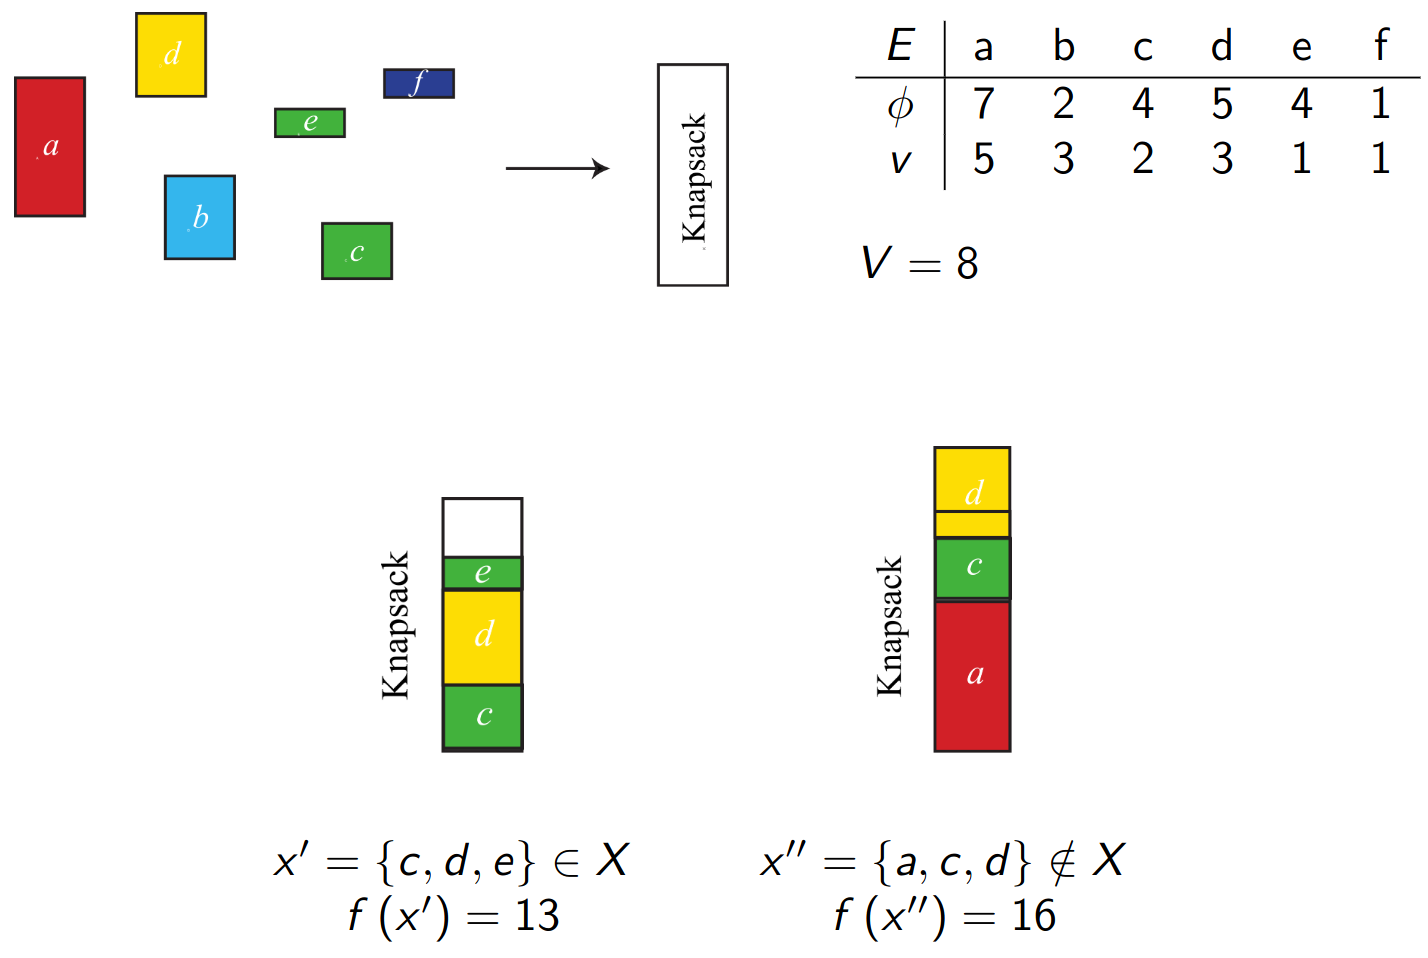
\includegraphics[width=\columnwidth]{img/KP1}
	\end{center}
	The left one is a solution, while the one on the right is not (or it can be called an unfeasible solution).
	
	\newpage
	
	\subsection{Set problems in metric spaces}
	\subsubsection{Maximum Diversity Problem (MDP)}
	Select the $k$ points with the maximum distance between each other.\\ 
	Select \textbf{from a set of points} a \textbf{subset} of $k$ points with the\textbf{ maximum sum of all pairwise distances}. It consists of: 
	\begin{itemize}
		\item a \textbf{set} $P$ of \textbf{points}
		\item a function $d: \, P \times P \rightarrow \mathbb{N}$ providing the \textbf{distance between point pairs}
		\item a number $k \in \left\{1, \, ... \, , |P| \right\}$ that is the \textbf{number of points} to select
	\end{itemize}
	
	The \textbf{ground set} is the set of \textbf{points} $B = P$.\\
	
	The \textbf{feasible region} includes all \textbf{subset} of $k$ \textbf{points} 
	$$ X = \left\{x \in B : \, |x| = k \right\}$$
	
	The \textbf{objective} is to \textbf{maximize the sum} of all pairwise \textbf{distances} between the selected points
	$$ \max_{x \in X} f(x) = \sum_{(i,j):i,j \in x} d_{ij}$$ 
	
	\paragraph{Example}
	\begin{center}
		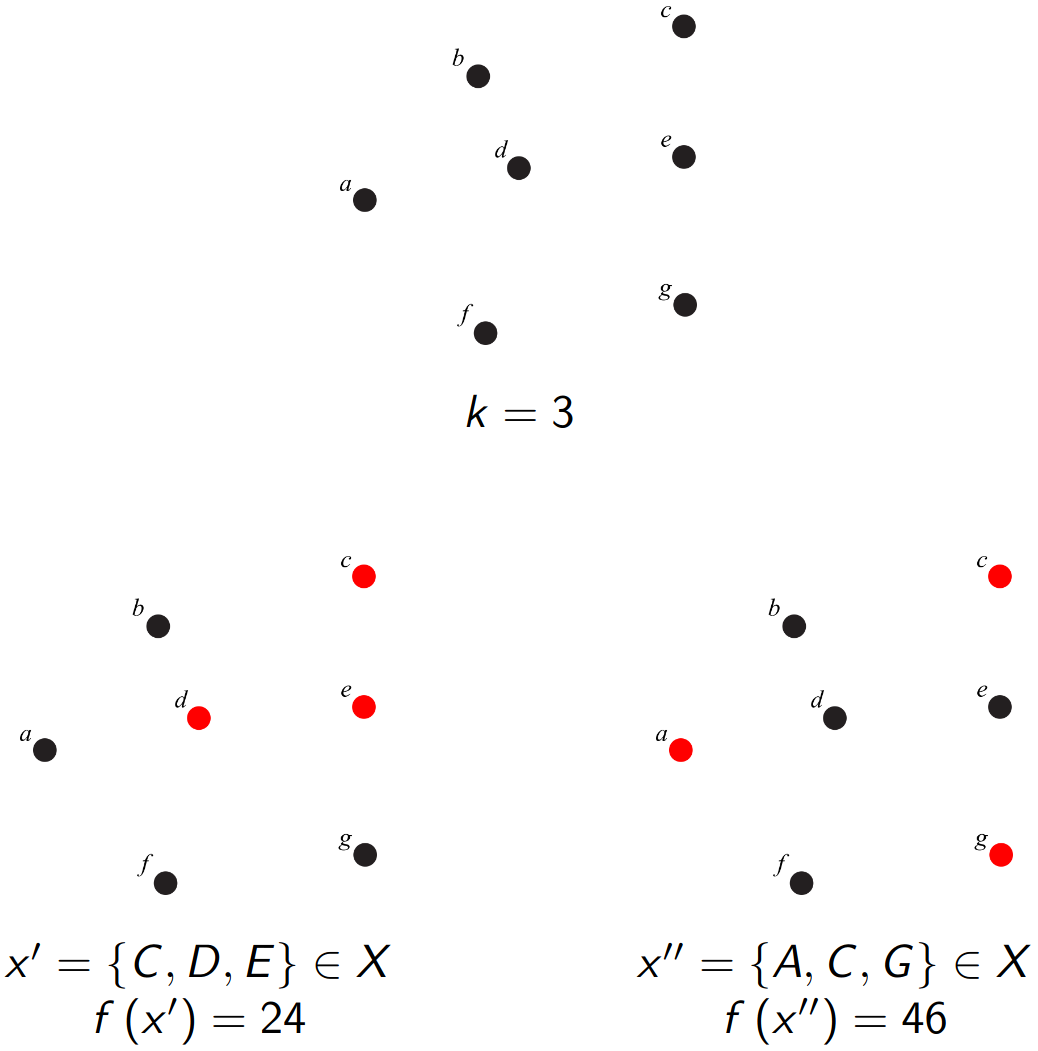
\includegraphics[width=0.6\columnwidth]{img/MDP1}
	\end{center}
	
	\newpage
	
	\subsection*{Interlude 1: The objective function}
	\addcontentsline{toc}{subsection}{Interlude 1: The objective function}
	%\addcontentsline{toc}{subsection}{\protect\numberline{}Interlude: The objective function}
	The \textbf{objective function} associates \textbf{integer values} to \textbf{feasible subjects}
	$$ f: \, X \rightarrow \mathbb{N} $$
	Computing the objective function can be complex (and exhausting).\\
	
	In the cases seen before: 
	\begin{itemize}
		\item the KP has an \textbf{additive} function which sums values of a function defined on the ground set (each element only has its own value)
		$$ \phi : \, B \rightarrow \mathbb{N} \text{ induces } f(x) \sum_{j \in x} \phi_j : \, X \rightarrow \mathbb{N} $$
		the additive function is easy to recompute if the subset $x$ changes, just sum each element added and subtract each element removed.\\
		
		\item the MDP has a \textbf{quadratic} objective function (each point needs to have the distance to every other element). \\
		The process for recomputing, when the subset changes, is more complex, but still quadratic in nature.\\
	\end{itemize}
	Both of these functions are defined not only on $X$ but on the whole $2^B$ (is it useful?).\\
	
	\newpage
	
	\subsection{Partitioning set problems}
	\subsubsection{Bin Packing Problem (BPP)}
	Put a set of objects in the minimum possible number of containers of a given volume.\\ 
	Divide a \textbf{set of voluminous objects} into the \textbf{minimum number of containers} of given capacity. It consists of:
	\begin{itemize}
		\item a set $E$ of \textbf{elementary objects}
		\item a function $v: \, E \rightarrow \mathbb{N}$ describing the \textbf{volume of each object}
		\item a set $C$ of \textbf{containers}
		\item a number $V \in \mathbb{N}$ that is the \textbf{volume of the containers}
	\end{itemize}
	
	The \textbf{ground set} includes all \textbf{(object, container) pairs}, $B = E \times C$.\\
	
	The \textbf{feasible region} includes all \textbf{partitions} of the \textbf{objects} among the \textbf{containers} not exceeding the capacity of any container
	$$ X = \left\{ x \subseteq B : \, |x \cap B_e| = 1 \;\; \forall e \in E, \sum_{(e,c) \in B^c} v_e \leq V \;\; \forall c \in C \right\}$$
	with $B_e \left\{(i,j) \in B : \, i = e\right\}$ and $B^c = \{(i,j) \in B : \, j = c \}$ (respectively, pairs in relation to the elements and pairs in relation to the containers).\\
	
	The \textbf{objective} is to \textbf{minimize the number of containers} used
	$$ \min_{x \in X} f(x) = \left| \left\{c \in C : \, x \cap B^c \neq \emptyset \right\}\right| $$
	the cardinality of the set of containers $C$ such that the pairs of the solution intersect $B^c$ in at least one element (not empty).\\
	
	\newpage
	
	\paragraph{Example}
	\begin{center}
		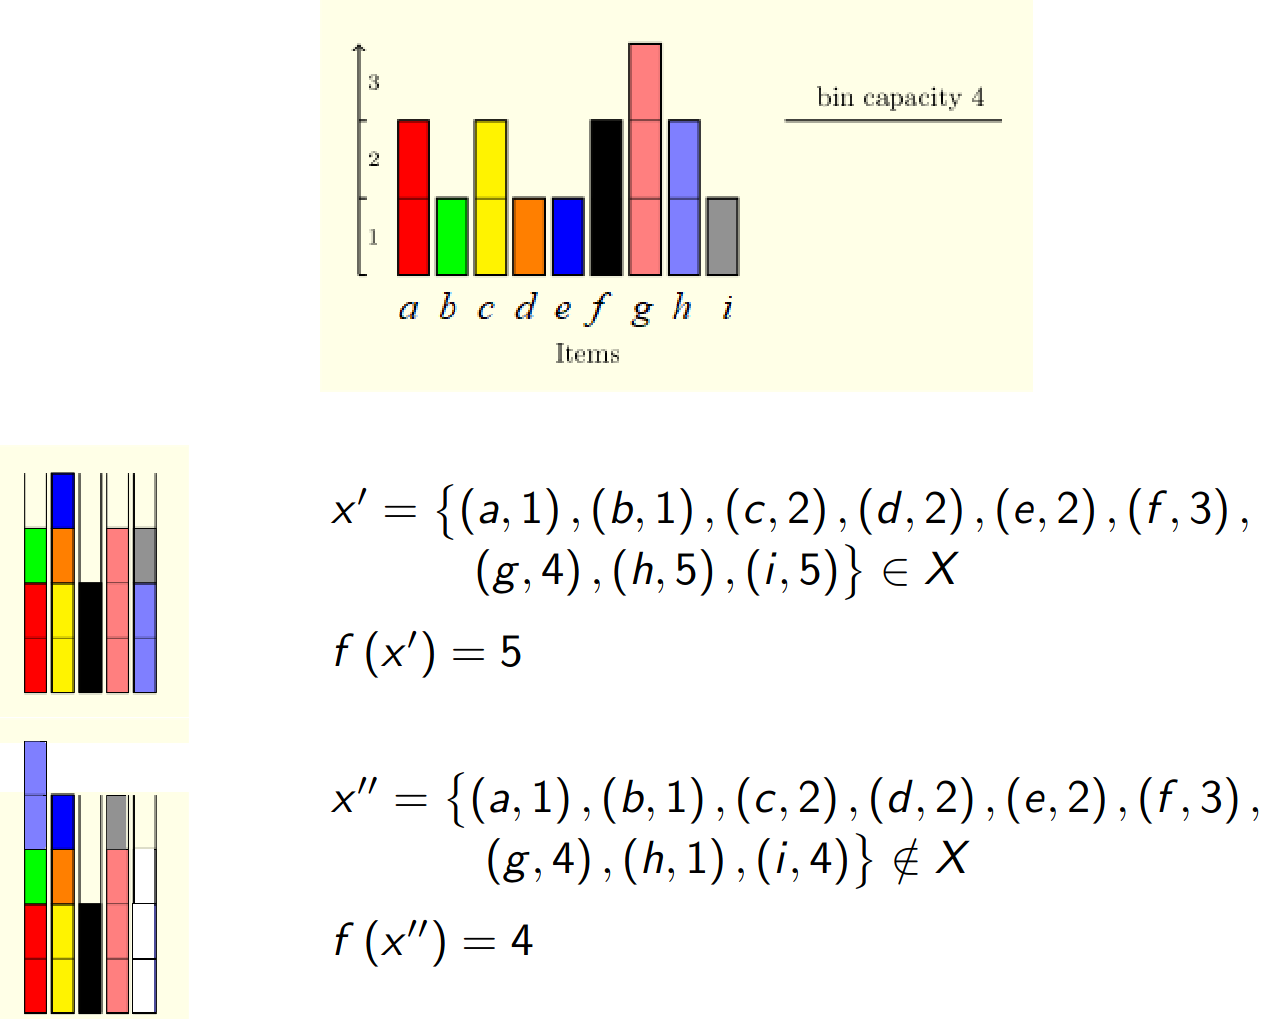
\includegraphics[width=\columnwidth]{img/BPP1}
	\end{center}
	In the first solution there is only a single pair for each item and the capacity of each container is not exceeded so it's a valid solution.
	
	\newpage
	
	\subsection{Parallel Machine Scheduling Problem (PMSP)}
	Divide a \textbf{set of tasks} among a \textbf{set of machines} \textbf{minimizing the completion time}. It consists of: 
	\begin{itemize}
		\item a set $T$ of \textbf{tasks}
		\item a function $d : T \rightarrow \mathbb{N}$ describing the \textbf{time length of each task}
		\item a set $M$ of \textbf{machines}
	\end{itemize}
	divide the tasks among the machines with the minimum completion time, each task to one machine only.\\
	
	The \textbf{ground set} includes all \textbf{(task,machine) pairs}, $B = T \times M$.\\
	
	The \textbf{feasible region} includes all \textbf{partitions of tasks among machines} (the order of the tasks is irrelevant, sum is the same)
	$$ X = \left\{x \subseteq B : \, |x \cap B_t| = 1 \;\; \forall t \in T \right\}$$
	
	The \textbf{objective} is to \textbf{minimize the maximum sum of time lengths} for each machine
	$$ \min_{x \in X} f(x) = \max_{m \in M} \sum_{t:(t,m) \in x} d_t $$
	this wants to minimize the maximum sum of duration for each machine in the solution; the final "value" (time spent) needs to be at a minimum and it is determined only by the longest-running machine.

	\newpage

	\paragraph{Example}
	\begin{center}
		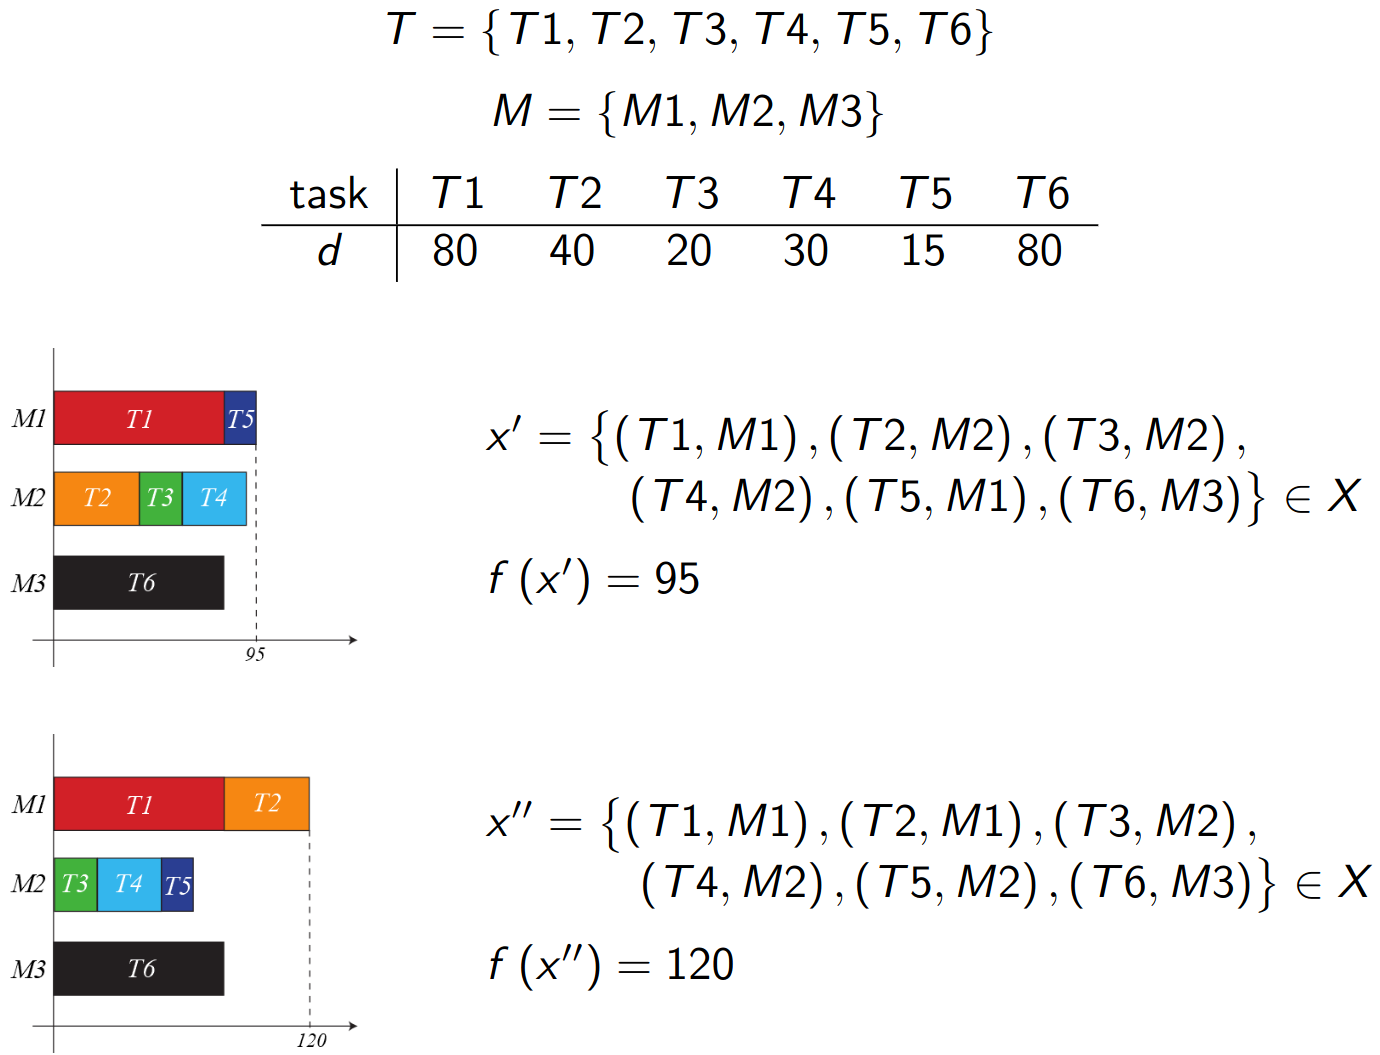
\includegraphics[width=\columnwidth]{img/PMSP}
	\end{center}
	The objective function wants to minimize the completion time, the value to complete the whole set of tasks, i.e. it wants to minimize the maximum time of a single machine.
	
	\newpage
	
	\subsection*{Interlude 2: The objective function again}
	\addcontentsline{toc}{subsection}{Interlude 2: The objective function again}
	The \textbf{ground set} is \textbf{not} always a single set, in the last examples was a cartesian product of two sets. \\
	
	The objective function for the BPP and PMSP is not additive and not trivial to compute. \\
	
	Small \textbf{changes} in the solution have a \textbf{variable impact} on the objective, it can be: 
	\begin{itemize}
		\item \textbf{equal} to the time length of the moved task (e.g., move $T5$ on $M1$ in $x''$)
		\item \textbf{zero} (e.g., move $T5$ on $M3$ in $x''$)
		\item \textbf{intermediate} (e.g., move $T2$ on $M2$ in $x''$)
	\end{itemize}
	The \textbf{impact} of a change to the solution \textbf{depends} both on the \textbf{modified} elements and the \textbf{unmodified} ones (contrary to the earlier interlude).\\
	
	The objective function is "flat", there are \textbf{several solutions} with the same \textbf{value} (is there a way to tell if a change is "good"?).\\
	
	\newpage
	
	\subsection{Logic function problems}
	\subsubsection{Max-SAT (satisfaction) problem}
	Given a \textit{CNF} (Conjunctive Normal Form), assign truth values to its logical variables so as to satisfy the \textbf{maximum weight subset of its logical clauses}. It consists of: 
	\begin{itemize}
		\item a set $V$ of \textbf{logical variables} $x_j$ with values in $\mathbb{B} = \{0, 1\}$ (\textit{false}, \textit{true}); the variables taken into consideration, which can be true or false
		\item a \textbf{literal} $l_j$ is a function consisting of an \textbf{affirmed or negated variable}
		$$ l_j (x) \in \{x_j, \overline{x}_j\}$$
		\item a \textbf{logical clause} is a disjunction or \textbf{logical sum} (\textit{OR}) \textbf{of literals}
		$$ C_i (x) = l_{i,1} \vee \; ... \; \vee l_{i,n}$$
		\item a \textbf{conjunctive normal form} (\textit{CNF}) is a conjunction or \textbf{logical product} (\textit{AND}) \textbf{of logical formulae}
		$$ CNF (x) = C_1 \wedge \; ... \; \wedge C_n $$
		it's the (logic) product of (logic) sums (literals).\\
		\item to satisfy a logical function means to make it assume value 1
		\item a function $w$ provides the \textbf{weights} of the \textit{CNF} formulae
	\end{itemize}
	
	The \textbf{ground set} is the set of \textbf{all simple truth assignments}
	$$ B = V \times \mathbb{B} = \left\{(x_1, 0), (x_1, 1), \; ... \; , (x_n, 0), (x_n, 1)\right\}$$
	the cartesian product of the set of variables with the set of logical values.\\
	
	The \textbf{feasible region} includes all \textbf{subsets of simple assignments} that are:
	\begin{itemize}
		\item \textbf{complete}, every variable has at least one value
		\item \textbf{consistent}, every variable has at most one value
	\end{itemize}
	$$ X = \left\{x \subseteq B : \, |x \cap B_v| = 1 \; \forall v \in V \right\}$$
	with $B_{x_j} = \left\{(x_j, 0), (x_j, 1)\right\}$.\\
	
	The \textbf{objective} is to \textbf{maximize the total weight of the satisfied formulae}: 
	$$ \max_{x \in X} f(x) = \sum_{i:C_i(x) = 1} w_i $$
	This is defined only on feasible solutions (you HAVE to assign a value to a variable, it just might not be the Max-SAT solution).\\
	
	\paragraph{Example}
	\begin{itemize}
		\item Variables
		$$ V = \{x_1, x_2, x_3, x_4\} $$
		\item Literals
		$$ L = {x_1, \overline{x}_1, x_2, \overline{x}_2, x_3, \overline{x}_3, x_4, \overline{x}_4} $$
		\item Logical clauses
		$$ C_1 = \overline{x}_1 \vee x_2 \;\;\;\; ... \;\;\;\; C_7 = x_2 $$ 
		\item Conjunctive normal form
		$$CNF = (\overline{x}_1 \vee x_2) \wedge (\overline{x}_1 \vee x_3) \wedge (\overline{x}_1 \vee \overline{x}_3) \wedge (\overline{x}_2 \vee x_4) \wedge (\overline{x}_2 \vee \overline{x}_4) \wedge x_1 \wedge x_2 $$
		\item Weight function (uniform, all 1):
		$$ w_i = 1 \;\;\;\;\;\; i = 1, \; ... \; ,7 $$
	\end{itemize}
	$x = \{(x_1, 0), (x_2, 0), (x_3, 1), (x_4, 1)\}$ satisfies $f (x) = 5$ formulae out of $7$.\\
	Complementing a variable does not always change $f(x)$ ($x_1$ does, $x_4$ doesn't).\\
	
	\newpage
	
	\subsection{Numerical matrix problems}
	\subsubsection{Set Covering (SCP)}
	Given
	\begin{itemize}
		\item a \textbf{binary matrix} $A \in \mathbb{B}^{m,n}$ with \textbf{row set} $R$ and \textbf{column set} $C$
		\item column $j \in C$ \textbf{covers} row $i \in R$ when $a_{ij} = 1$
		\item a function $c :\, C \rightarrow \mathbb{N}$ provides the \textbf{cost of each column}
	\end{itemize}
	Select a \textbf{subset of columns covering all rows at minimum cost}.\\
	
	Essentially: there's a binary matrix (filled with 0s and 1s), each column has a cost, you need to get the minimum cost for covering all the rows, i.e. having at least one "1" value for each row.\\
	
	The \textbf{ground set} is the set of \textbf{columns}, $B = C$.\\
	
	The \textbf{feasible region} includes all \textbf{subsets} of \textbf{columns} that \textbf{cover all rows}
	$$ X \left\{ x \subseteq B : \, \sum_{j \in x} a_{ij} \geq 1 \; \forall i \in R \right\}$$
	All the solution subset of the columns such that there is at least a 1 ($a_{ij} \geq 1$) for all rows $i$.\\
	
	The \textbf{objective} is to \textbf{minimize} the total \textbf{cost} of the selected \textbf{columns}
	$$ \min_{x \in X} f(x) = \sum_{j \in x} c_j$$
	It's additive and is simply the cost of the columns.\\
	
	\newpage
	
	\paragraph{Example}
	\begin{center}
		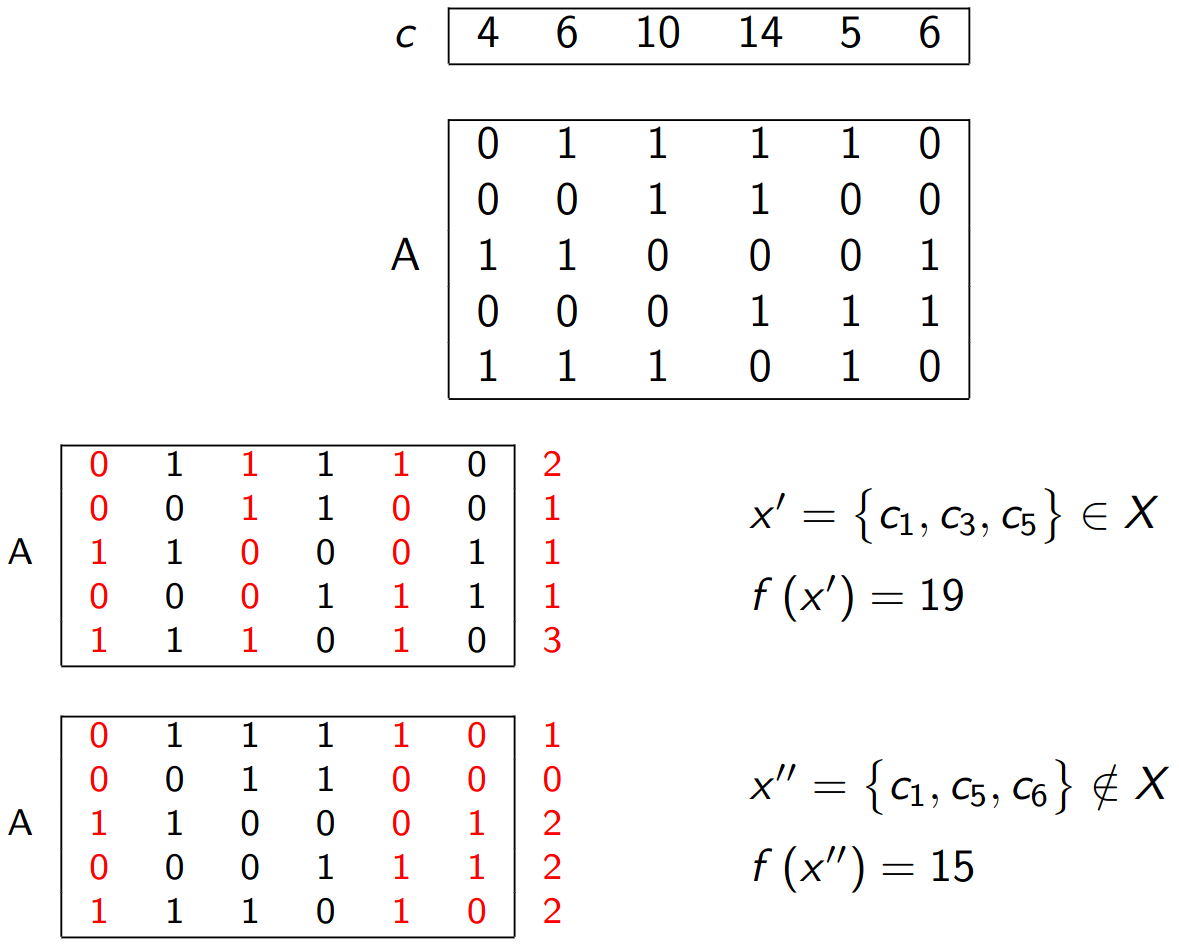
\includegraphics[width=\columnwidth]{img/SCP1}
	\end{center}
	The first one is a solution, the second one is unfeasible.\\
	
	"Set Covering": covering a set (rows) with subsets (columns).\\
	
	\newpage
	
	\subsection*{Interlude 3: The feasibility test}
	\addcontentsline{toc}{subsection}{Interlude 3: The feasibility test}
	Often heuristic algorithms require solving the problem "here is a subset of elements, \textbf{is it feasible?}" or in short "$x \in X$?". It's a decision problem.\\
	
	Sometimes is really easy (Max-SAT problem, just check that each variable appears exactly once), sometimes it's not as linear (SCP, you need the sum of each row, still easy but not as easy).\\
	
	The \textbf{feasibility test} requires to \textbf{compute from the solution} and test
	\begin{itemize}
		\item \textbf{a single number:} the total volume (KP), the cardinality (MDP)
		\item \textbf{a single set of numbers:} values assigned to each variable (Max-SAT), number of machines for each task (PMSP)
		\item \textbf{several sets of numbers:} number of containers for each object and total volume of each container (BPP)
	\end{itemize}
	\nn
	
	The time required can be \textbf{different} if the test is performed
	\begin{itemize}
		\item \textbf{from scratch} on a generic subset $x$
		\item on a \textbf{subset} $x'$ obtained by slightly \textbf{modifying} a feasible solution $x$
	\end{itemize}
	\nn
	
	Some modifications can be forbidden \textit{a priori} to avoid infeasibility (insertions and removals for MDP, PMSP, Max-SAT), while others require an \textit{a posteriori} test (exchanges). Some families of modification can be ruled out.\\
	
	% End of L1P2
	
	\newpage
	
	\subsection{Numerical matrix problems}
	\subsubsection{Set Packing}
	Given:
	\begin{itemize}
		\item a \textbf{binary matrix} $A \in \mathbb{B}^{m,n}$ with \textbf{row set} $R$ and \textbf{column set} $C$
		\item \textbf{columns} $j'$ e $j'' \in C$ \textbf{conflict} with each other when $a_{ij'} = a_{ij''} = 1$
		\item a function $\phi : \, C \rightarrow \mathbb{N}$ provides the \textbf{value of each column}
	\end{itemize}
	Select a \textbf{subset} of \textbf{nonconflicting columns} of \textbf{maximum value}.\\
	There can't be two 1s in the same row of two chosen columns; the sum of all values in each row must be $\leq 1$.\\
	
	The \textbf{ground set} is the set of \textbf{columns}, $B = C$.\\
	
	The \textbf{feasible region} includes all \textbf{subsets} of \textbf{nonconflicting columns}
	$$ X = \left\{x \subseteq B: \, \sum_{j \in x} a_{ij} \leq 1 \; \forall i \in R \right\}$$
	
	The \textbf{objective} is to \textbf{maximize the total value} of the selected columns
	$$ \max_{x \in X} f(x) = \sum_{j \in x} \phi_j $$
	
	\newpage
	
	\paragraph{Example}
	\begin{center}
		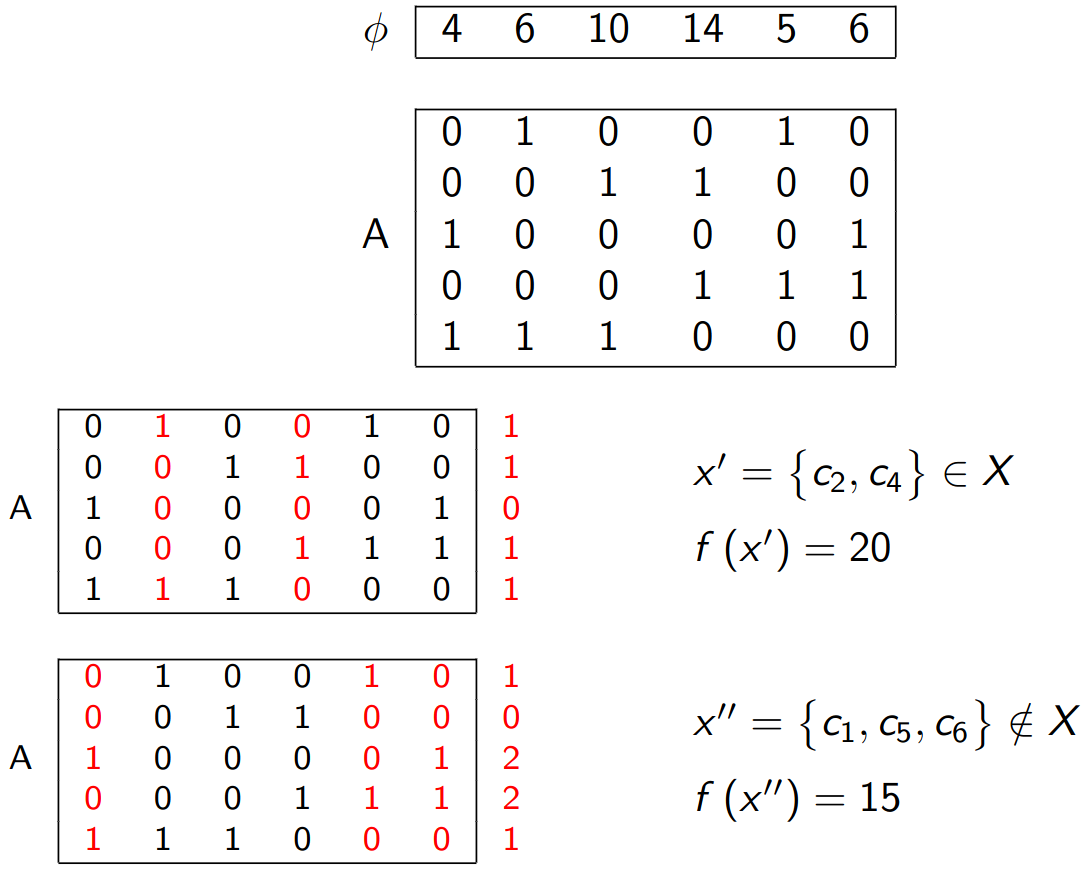
\includegraphics[width=\columnwidth]{img/SetPacking1}
	\end{center}
	The first one is a feasible solution, while the second one is not feasible (the sum two of the rows is $>1$).\\
	
	"Set Packing": packing disjoint subsets (columns) of a set (rows).\\
	
	\newpage
	
	\subsubsection{Set Partitioning (SPP)}
	Given a binary matrix and a cost function defined on its columns, select a \textbf{minimum cost} subset of \textbf{nonconflicting columns covering all rows}. It consists of:
	\begin{itemize}
		\item a \textbf{binary matrix} $A \in \mathbb{B}^{m,n}$ with a \textbf{set of rows} $R$ and a \textbf{set of
		columns} $C$
		\item a function $c : \, C \rightarrow \mathbb{N}$ that provides the \textbf{cost of each column}
	\end{itemize}
	similar to the last problems, the difference is that the sum in each row must be exactly $= 1$; cover each row exactly once, not at least once (SCP) or at most once (Set Packing).\\
	
	The \textbf{ground set} is the set of columns, $B = C$.\\
	
	The \textbf{feasible region} includes all subsets of \textbf{columns} that \textbf{cover all rows} and are \textbf{not conflicting}
	$$ X = \left\{x \subseteq C : \, \sum_{j \in x} a_{ij} = 1 \; \forall i \in R \right\}$$
	
	The \textbf{objective} is to \textbf{minimize} the total \textbf{cost} of the selected \textbf{columns}
	$$ \min_{x \in X} f(x) = \sum_{j \in x} c_j $$
	
	\newpage
	
	\paragraph{Example}
	\begin{center}
		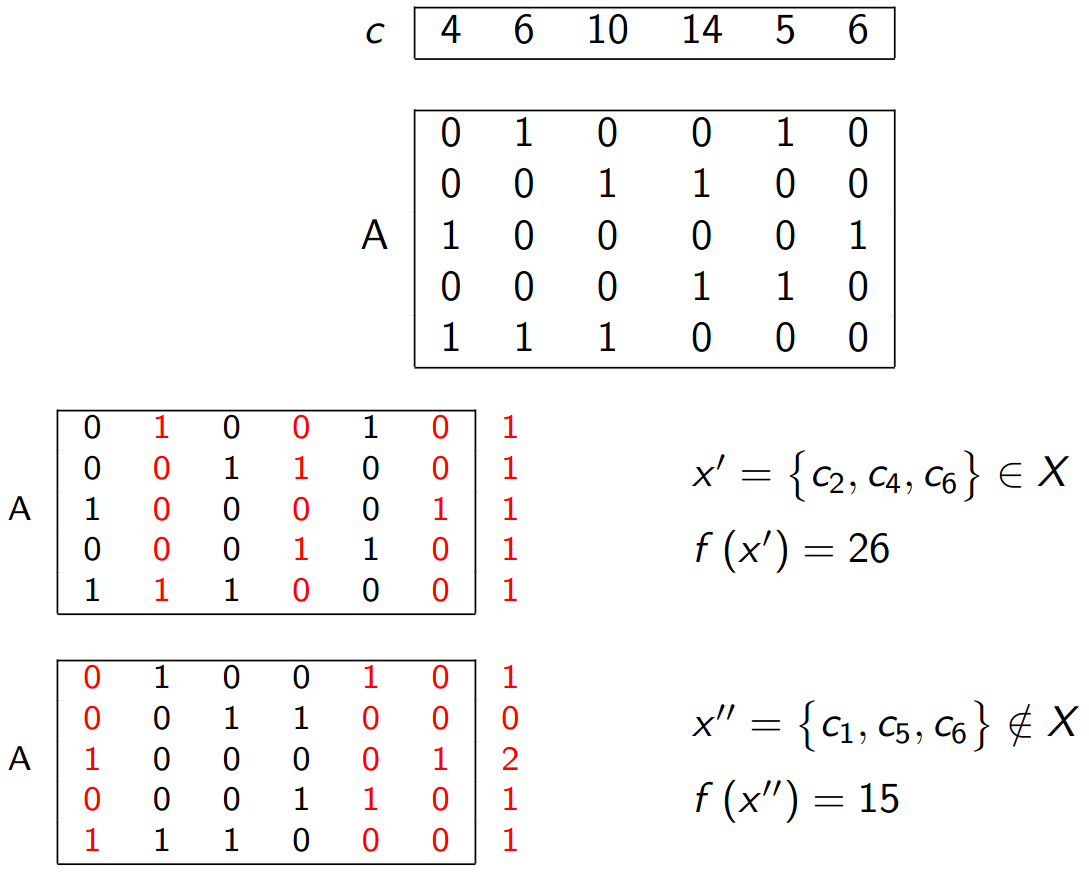
\includegraphics[width=\columnwidth]{img/SPP1}
	\end{center}
	The first one is a feasible solution, while the second one is not feasible (the sum of a row is $0$, while another one is $2$).\\
	
	"Set Partitioning": partition a set (rows) into subsets (columns).\\
	
	\newpage
	
	\subsection*{Interlude 4: The search for feasible solutions}
	\addcontentsline{toc}{subsection}{Interlude 4: The search for feasible solutions}
	Heuristic algorithms often require to solve the problem "\textbf{Find a feasible solution} $x \in X$", it's a search problem. \\
	
	\textbf{Depending} on the problem, the solution can be \textbf{trivial}: 
	\begin{itemize}
		\item some sets are \textbf{always feasible}, such as $x = \emptyset$ (KP, Set Packing) or $x = B$ (feasible instances of SCP)
		\item random solutions satisfying a \textbf{constraint}, such as $|x| = k$ (MDP, doesn't matter which points, you can take $k$ random points)
		\item random solutions satisfying \textbf{consistency constraints}, such as assigning one task to each machine (PMSP), one value to each logic variable (Max-SAT), etc.; a random assignment (in both cases) can be s feasible solution, it might be a bad solution, but feasible
	\end{itemize}
	but it can also be \textbf{hard}:
	\begin{itemize}
		\item in the BPP the number of containers must be sufficiently large (e.g., provide one container for each object, then minimize)
		\item in the SPP no polynomial algorithm is known to solve the problem
	\end{itemize}
	Some algorithms \textbf{enlarge the feasible region} from $X$ to $X'$ (relaxation)
	\begin{itemize}
		\item the \textbf{objective} $f$ must be \textbf{extended} from $X$ to $X'$ (sometimes it's possible, sometimes it's not, see first interlude)
		\item but often $X' \setminus X$ includes better solutions; the new solutions could be better (obviously, we are relaxing the constraints, the objective function can be better for unfeasible solutions)
	\end{itemize}
	
	\newpage
	
	\subsection{Graph problems}
	\subsubsection{Vertex Cover (VCP)}
	Given an \textbf{undirected graph}, select a \textbf{subset of vertices of minimum cardinality} such that \textbf{each edge of the graph is incident to it}. It consists of:
	\begin{itemize}
		\item an \textbf{undirected graph} $G = (V,E)$
	\end{itemize}
	The goal is to get every node adjacent to at least one selected node.\\
	The problem can be weighted by adding a weight function to each node instead of considering unitary value.\\
	
	The \textbf{ground set} is the \textbf{vertex set}, $B = V$.\\
	
	The \textbf{feasible region} includes \textbf{all vertex subsets} such that \textbf{all the edges} of the graph \textbf{are incident to them}
	$$ X = \left\{x \subseteq V : \, x \cap (i,j) \neq \emptyset \; \forall (i,j) \in E \right\}$$
	all the subsets of vertices such as the intersection between this and every possible pair of edges is not empty, i.e. there must be every pair of vertices in the solution.
	
	The \textbf{objective} is to \textbf{minimize} the \textbf{number of} selected \textbf{vertices}
	$$ \min_{x \in X} f(x) = |x| $$
	
	It becomes the sum of the weight of the vertices if we have a weight function $w$
	$$ \min_{x \in X} f(x) = \sum_{j \in x} w_j $$
	
	\newpage
	
	\paragraph{Example}
	\begin{center}
		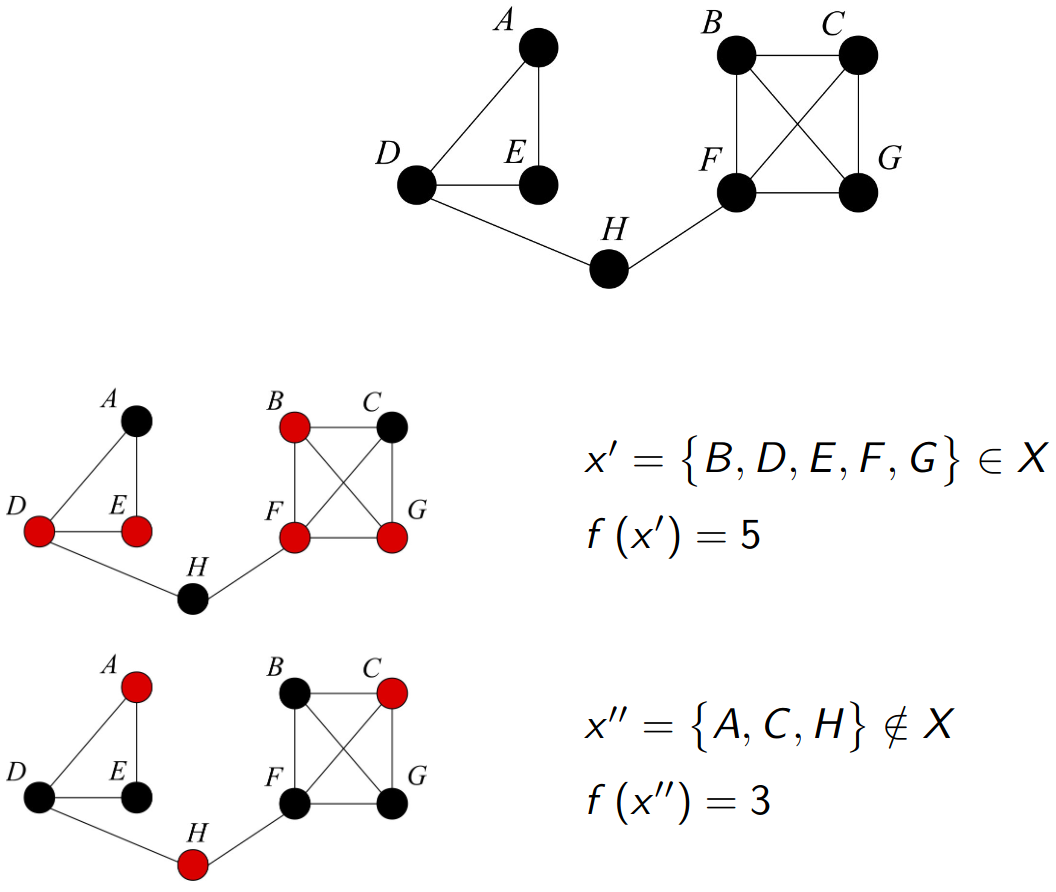
\includegraphics[width=\columnwidth]{img/VCP1}
	\end{center}
	The first one is a solution, the second one is unfeasible since there are some edges missing.\\
	As the last interlude predicted, the unfeasible solution has a better value than the feasible one.\\
	
	\newpage
	
	\subsubsection{Maximum Clique Problem}
	Given:
	\begin{itemize}
		\item an \textbf{undirected graph} $G = (V , E )$
		\item a function $w : V \rightarrow \mathbb{N}$ that provides the weight of each vertex
	\end{itemize}
	select the subset of \textbf{pairwise adjacent vertices of maximum weight}.\\
	The problem consists in finding the subset of adjacent vertices (a clique, each vertex is connected by an edge to every other node) of maximum weight.\\
	
	The \textbf{ground set} is the \textbf{vertex set}, $B = V$.\\
	
	The \textbf{feasible region} includes all \textbf{subsets of pairwise adjacent vertices}
	$$ X = \left\{x \subseteq V : \, (i,j) \in E \; \forall i \in x, \, \forall j \in X \setminus \left\{i\right\}\right\}$$
	for any pair of vertices belonging to the solution the pair itself belongs to the edge set.\\
	
	The \textbf{objective} is to \textbf{maximize} the \textbf{weight} of the selected vertices
	$$ \max_{x \in X} f(x) = \sum_{j \in x} w_j $$
	
	\newpage
	
	\paragraph{Example}
	\begin{center}
		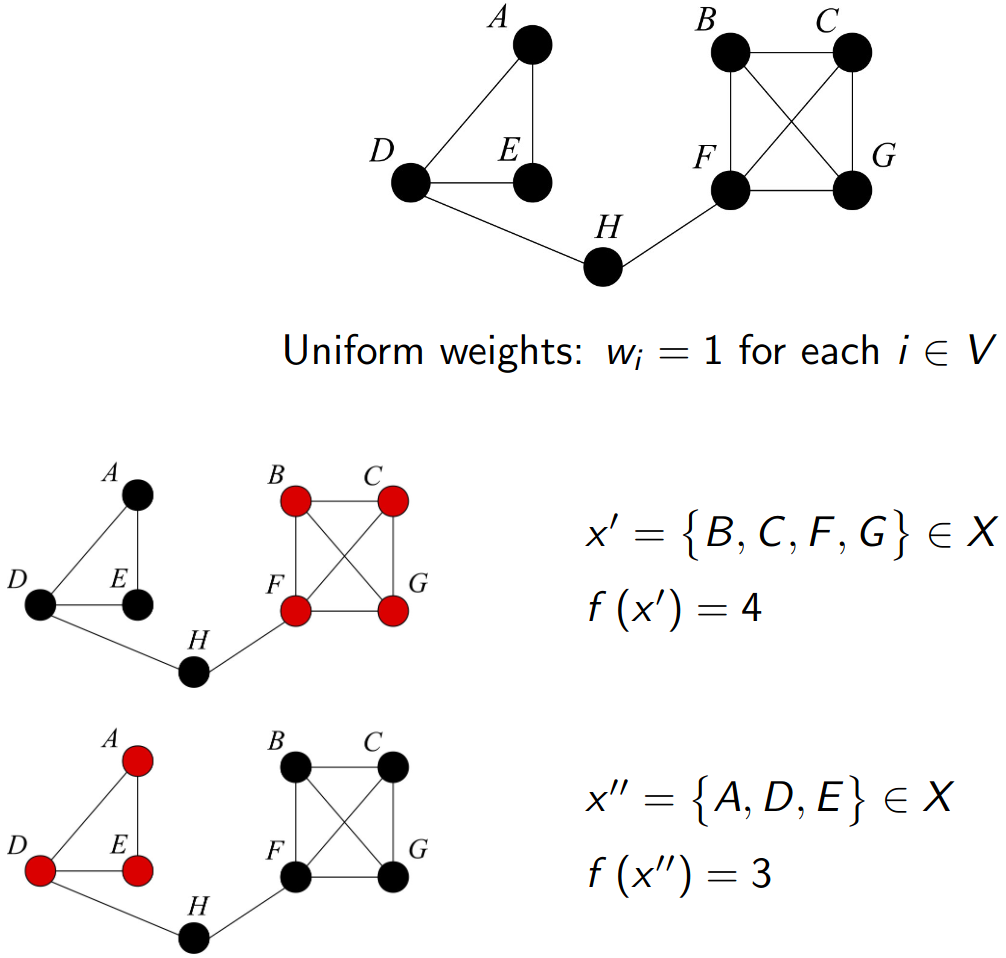
\includegraphics[width=\columnwidth]{img/MCP1}
	\end{center}
	
	\newpage
	
	\subsubsection{Maximum Independent Set Problem}
	Given
	\begin{itemize}
		\item an \textbf{undirected graph} $G = (V , E )$
		\item a function $w : V \rightarrow \mathbb{N}$ that provides the \textbf{weight of each vertex}
	\end{itemize}
	select the \textbf{subset of pairwise nonadjacent vertices of maximum weight}.\\
	The subset of not connected nodes with the maximum weight.\\
	
	The \textbf{ground set} is the \textbf{vertex set}, $B = V$.\\
	
	The \textbf{feasible region} includes the subsets of \textbf{pairwise nonadjacent vertices}
	$$ X = \left\{x \subseteq B : \, (i,j) \notin E \; \forall i \in x, \, \forall j \in x \setminus \left\{i\right\}\right\}$$
	
	The \textbf{objective} is to \textbf{maximize the weight} of the selected vertices
	$$ \max_{x \in X} f(x) = \sum_{j \in x} w_j $$
	
	\newpage
	
	\paragraph{Example}
	\begin{center}
		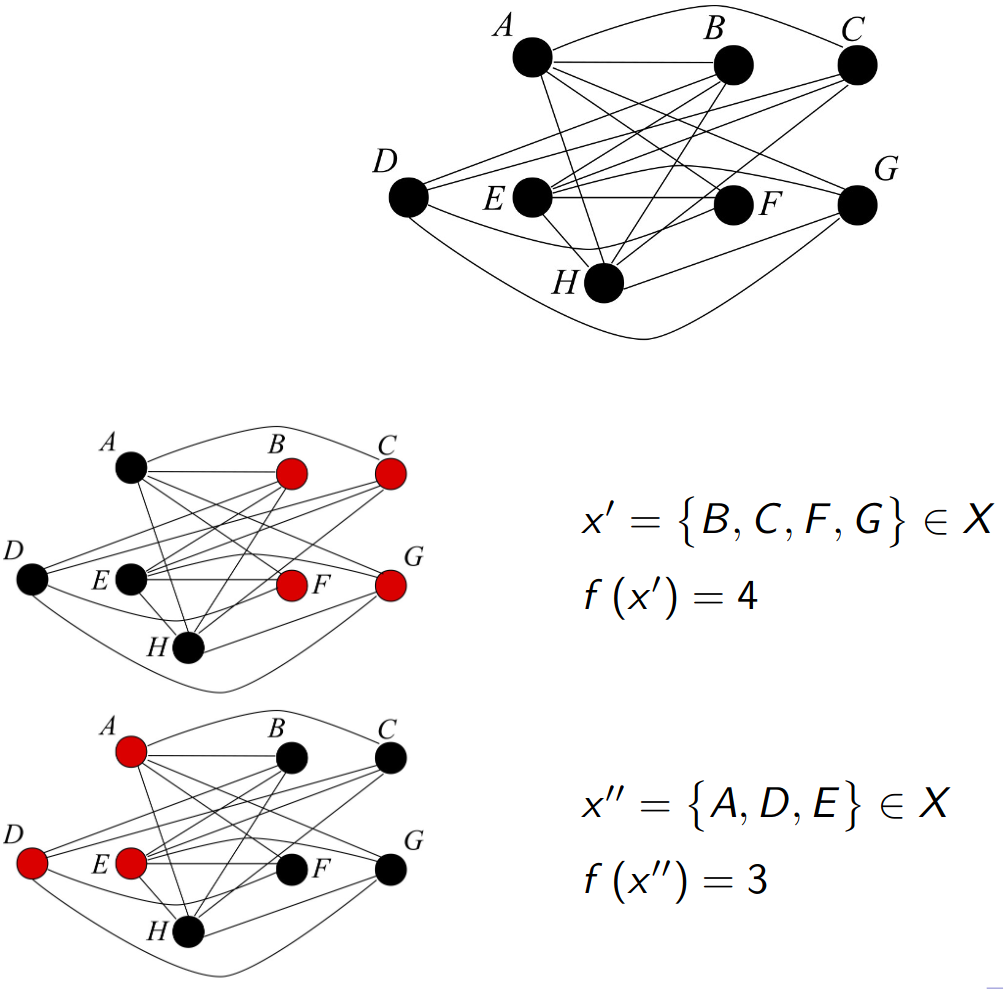
\includegraphics[width=\columnwidth]{img/MISP1}
	\end{center}
	
	\newpage
	
	\subsection*{Interlude 5: The relations between problems}
	\addcontentsline{toc}{subsection}{Interlude 5: The relations between problems}
	\label{I5}
	Each instance of the \textbf{MCP} is \textbf{equivalent} to an instance of the \textbf{MISP}:
	\begin{enumerate}
		\item start from the MCP instance, that is graph $G = (V , E)$ \\
		\item build the complementary graph $\overline{G} = (V , (V \times V ) \setminus E )$ \\
		\item find an optimal solution of the MISP on $\overline{G}$ \\
		\item the corresponding vertices give an optimal solution of the MCP on $G$ (a heuristic MISP solution gives a heuristic MCP solution) \\
	\end{enumerate}
	\begin{center}
		\includegraphics[width=\columnwidth]{img/interlude5}
	\end{center}
	The process can also be applied in the \textbf{opposite} direction.\\
	
	The \textbf{solution of the MCP can be used to find the solution of the MISP}, and vice versa.\\
	There's no need to design two different algorithms since the same one works for both problems, with a simple transformation of the instance.\\
	
	\newpage
	
	The \textbf{VCP} and the \textbf{SCP} are also \textbf{related}, but in a different way; each instance of the VCP can be \textbf{transformed} into an \textbf{instance} of the SCP:
	\begin{itemize}
		\item each edge $i$ corresponds to a row of the covering matrix $A$
		\item each vertex $j$ corresponds to a column of $A$
		\item if edge $i$ touches vertex $j$, set $a_{ij} = 1$; otherwise $a_{ij} = 0$
		\item an optimal solution of the SCP gives an optimal solution of the VCP (a heuristic SCP solution gives a heuristic VCP solution)
	\end{itemize}
	\begin{center}
		\includegraphics[width=\columnwidth]{img/interlude52}
	\end{center}
	The reverse is not as simple, not every binary matrix can be turned into a graph.\\
	
	The VCP is equivalent to solving the SCP on a matrix that determines to which vertices every edge is connected to.\\
	
	\newpage
	
	The \textbf{BPP} and the \textbf{PMSP} are \textbf{equivalent}, but in a more sophisticated way:
	\begin{itemize}
		\item the \textbf{tasks} correspond to the \textbf{objects}
		\item the \textbf{machines} correspond to the \textbf{containers}, but
		\begin{itemize}
			\item BPP: minimise the number of containers, given the capacity
			\item PMSP: given the number of machines, minimise the completion time
		\end{itemize}
	\end{itemize}
	Start from a \textbf{BPP instance}
	\begin{enumerate}
		\item make an \textbf{assumption} on the optimal \textbf{number} of \textbf{containers} (e.g., 3)
		\item build the \textbf{corresponding PMSP} instance
		\item \textbf{compute} the \textbf{optimal} completion \textbf{time} (e.g., 95)
		\begin{itemize}
			\item if it \textbf{exceeds} the capacity (e.g., 80), increase the assumption (4 or 5)
			\item if it \textbf{does not}, decrease the assumption (2 or 1)
		\end{itemize}
		(using heuristic PMSP solutions leads to a heuristic BPP solution)
	\end{enumerate}
	
	\begin{center}
		\includegraphics[width=0.8\columnwidth]{img/interlude53}
	\end{center}
	
	The reverse process is \textit{possible}.\\
	
	The two problems are equivalent, but each one must be solved several times.\\
	
	\newpage
	
	\subsubsection{Traveling Salesman Problem (TSP)}
	Given:
	\begin{itemize}
		\item a \textbf{directed graph} $G = (N, A)$
		\item a function $c : \, A \rightarrow \mathbb{N}$ that provides the \textbf{cost of each arc}
	\end{itemize}
	select a \textbf{circuit} visiting \textbf{all the nodes} of the graph at \textbf{minimum cost}.\\
	
	The \textbf{ground set} is the \textbf{arc set}, $B = A$.\\
	
	The \textbf{feasible region} includes the \textbf{circuits} that \textbf{visit all nodes} in the graph (hamiltonian circuits).\\
	
	How to determine whether a subset is a feasible solution? \\
	And a modification of a feasible solution? \\
	Can some modifications be ruled out? \\
	Finding an hamiltonian circuit is usually NP-hard, it's trivial only in the case of a connected graph. \\
	
	The \textbf{objective} is to \textbf{minimize} the \textbf{total cost} of the selected arcs
	$$ \min_{x \in X} f(x) = \sum_{j \in x} c_j $$
	
	\newpage
	
	\paragraph{Example}
	\begin{center}
		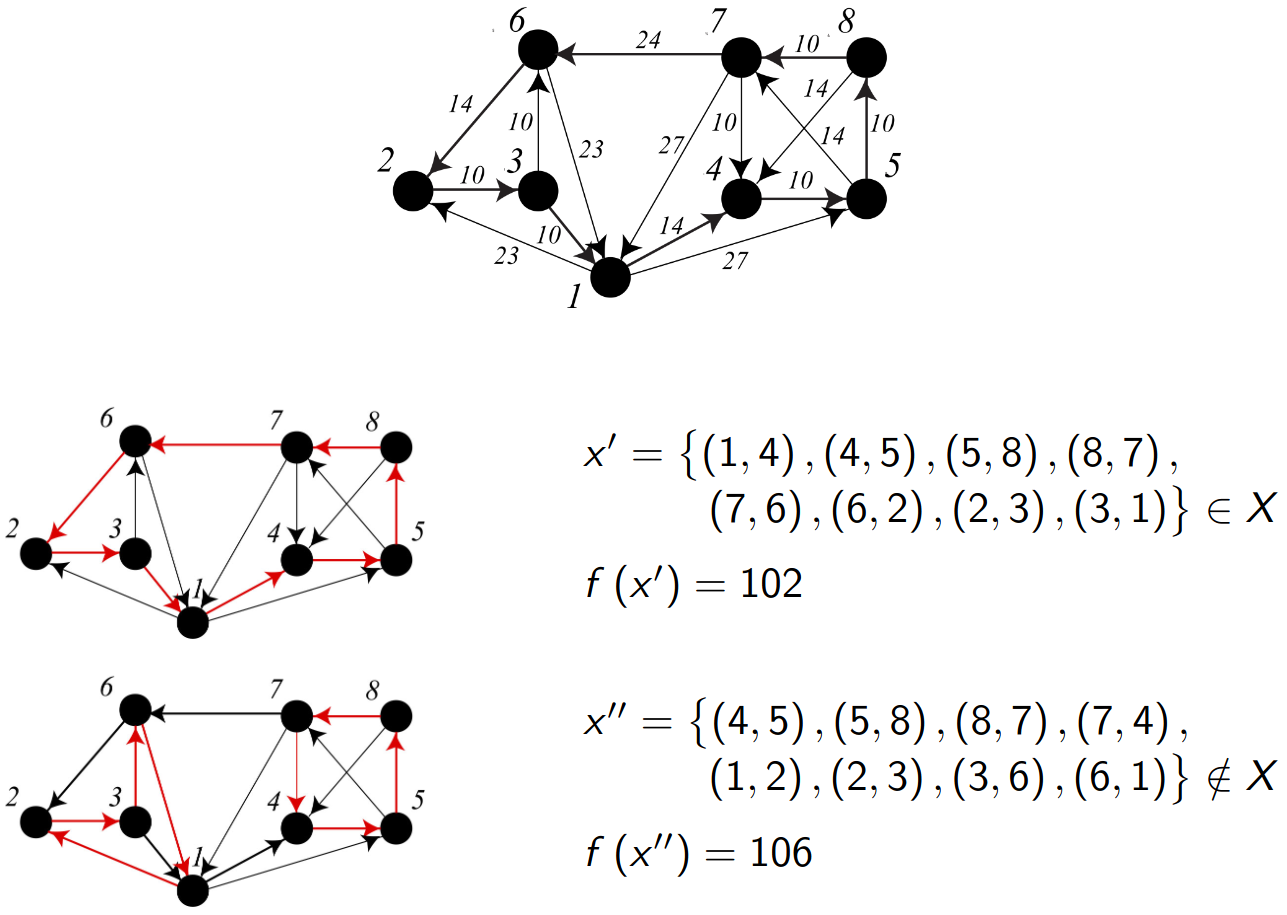
\includegraphics[width=\columnwidth]{img/TSP1}
	\end{center}
	The first one is a solution, the second one isn't because although it visits all the vertices there are 2 different sub-circuits.\\
	
	\newpage
	
	\subsubsection{Capacitated Min. Spanning Tree Problem}
	Given
	\begin{itemize}
		\item an \textbf{undirected graph} $G = (V , E )$ with a \textbf{root vertex} $r \in V$
		\item a function $c : \, E \rightarrow \mathbb{N}$ that provides the \textbf{cost of each edge}
		\item a function $w : \, V \rightarrow \mathbb{N}$ that provides the \textbf{weight of each vertex}
		\item a number $W \in \mathbb{N}$ that is the \textbf{subtree appended to the root} (branch), i.e. capacity of each subtree
	\end{itemize}
	select a \textbf{spanning tree} of \textbf{minimum cost} such that each \textbf{branch respects the capacity}.\\
	Find a spanning tree starting from a root node $r$, each branch must be under the limit weight (not too many vertices, must be under $W$).\\
	
	The \textbf{ground set} is the \textbf{edge set}, $B = E$.\\
	
	The \textbf{feasible region} includes \textbf{all spanning trees} such that the \textbf{weight of the vertices} spanned by each branch \textbf{does not exceed} $W$.\\
	The feasibility test requires to visit the subgraph.\\
	
	The \textbf{objective} is to \textbf{minimize} the \textbf{total cost} of the selected edges
	$$ \min_{x \in X} f(x) = \sum_{j \in x} c_j $$
	
	\newpage
	
	\paragraph{Example}
	\begin{center}
		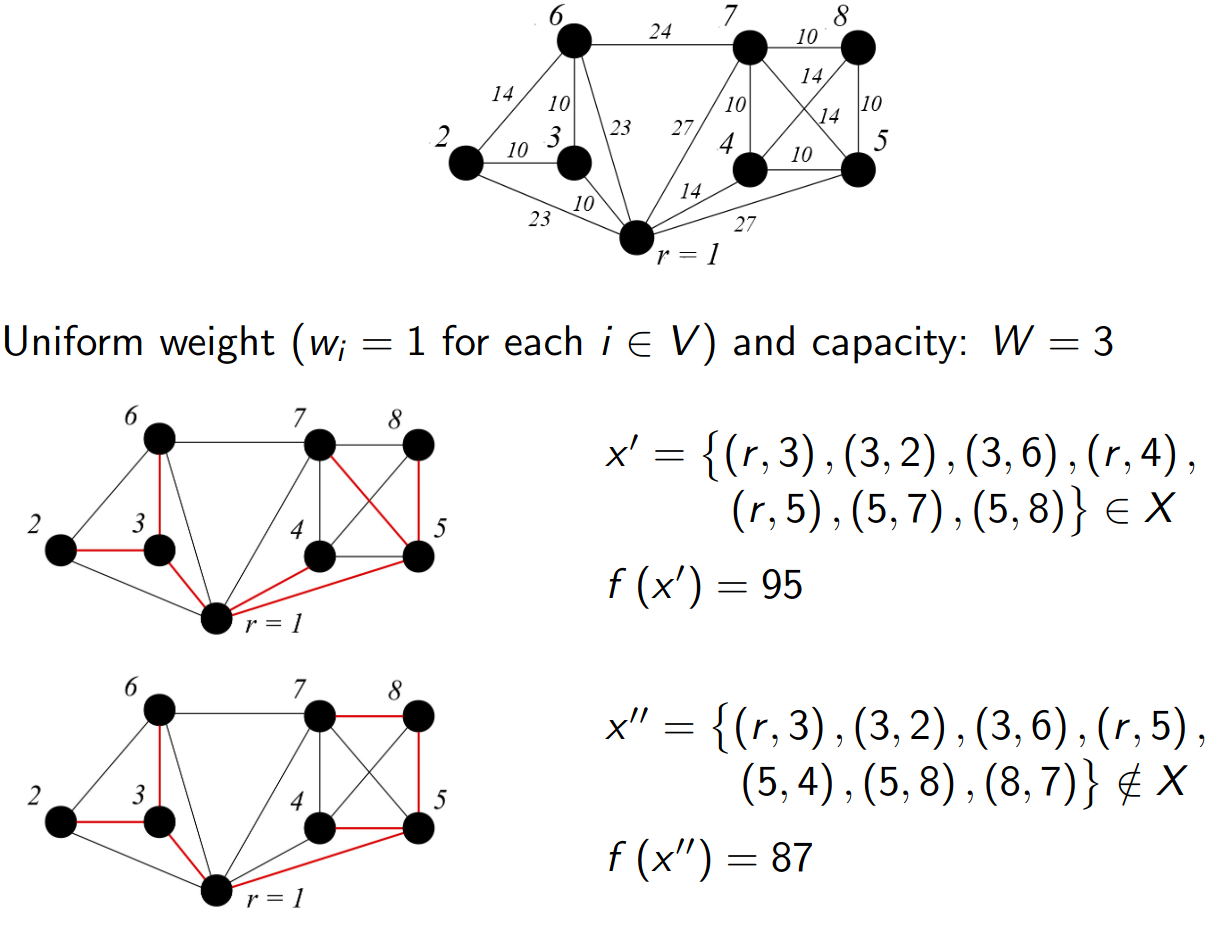
\includegraphics[width=0.8\columnwidth]{img/CSTP}
	\end{center}
	It is easy to evaluate the objective, less easy the feasibility.
	
	\paragraph{Cost of the main operation:} the objective function is:
	\begin{itemize}
		\item \textbf{fast to evaluate:} sum the edge cost
		\item \textbf{fast to update:} sum the added costs and subtract the removed ones
	\end{itemize}
	but it's easy to generate nonoptimal subtrees given the covered vertices.\\
	
	The \textbf{feasibility test} is
	\begin{itemize}
		\item \textbf{not} very \textbf{fast to perform:} 
		\begin{itemize}
			\item visit to check for connection and acyclicity
			\item visit to compute the total weight of each subtree
		\end{itemize}
		\item \textbf{not} very \textbf{fast to update:} 
		\begin{itemize}
			\item show that the removed edges break the loops introduced by the added ones
			\item recompute the weights of the subtrees
		\end{itemize}
	\end{itemize}
	This also holds when the graph is complete.\\
	
	What if we described the problem in terms of vertex subsets?
	
	\newpage
	
	\paragraph{Alternative description:} define a set of \textbf{subtrees} $T$ (as in the containers in the BPP), one for each vertex in $V \setminus \left\{r\right\}$: some can be empty.\\
	
	The \textbf{ground set} is the \textbf{set of the (vertex,branch) pairs}, $B = V \times T$.\\
	
	The \textbf{feasible region} includes \textbf{all partitions of the vertices into connected subsets} (visit, trivial on complete graphs) \textbf{of weight} $\leq W$ (as in the BPP)
	$$ X = \left\{x \subseteq B : \, |x \cap B_v| = 1 \; \forall v \in V \setminus \left\{r\right\}, \, \sum_{(i,j)\in B^t} w_i \leq W \; \forall t \in T, \; ... \; \right\}$$
	with $B_v = {(i, j) \in B : \, i = v }$, $B^t = {(i, j) \in B : j = t}$.\\
	
	The \textbf{objective} is to \textbf{minimize} the \textbf{sum of the costs of the branches} spanning each subset of vertices and appending it to the root.\\
	It is a combination of minimum spanning tree problems.\\
	
	The previously considered solutions now have a \textbf{different representation}.
	\begin{center}
		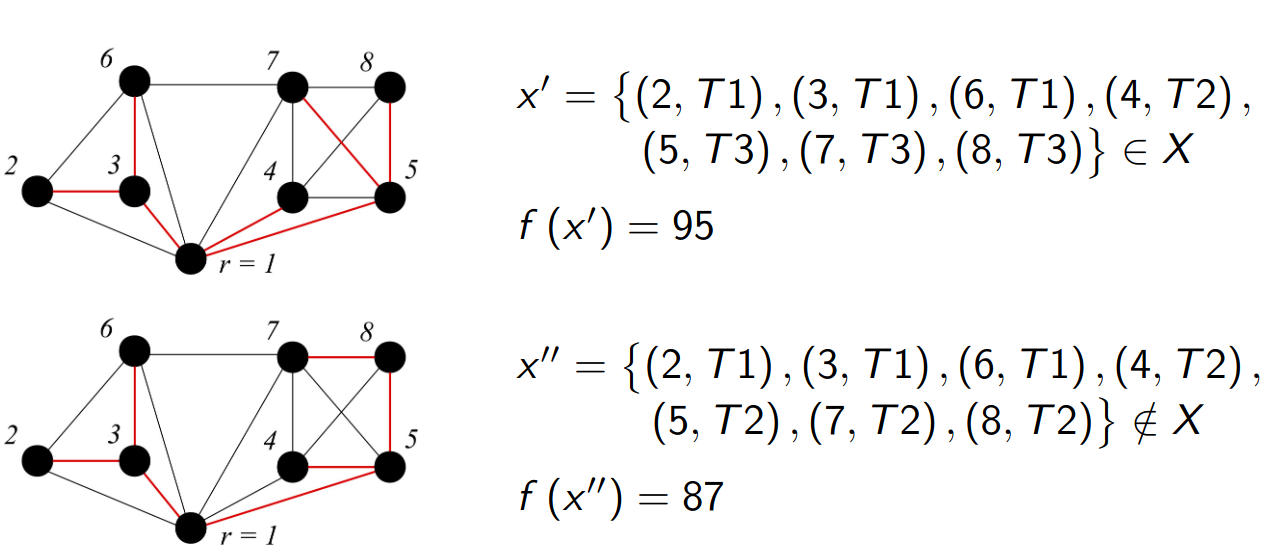
\includegraphics[width=0.9\columnwidth]{img/CSTP2}
	\end{center}
	The feasibility test only requires to sum the weights, computing the objective requires to solve a MST problem.
	
	\newpage
	
	\paragraph{New cost of operations:} the objective function is
	\begin{itemize}
		\item \textbf{slow to evaluate:} compute a MST for each subset
		\item \textbf{slow to update:} recompute the MST for each modified subset
	\end{itemize}
	but the subtrees are \textbf{optimal by construction}.\\
	
	If the graph is complete, the \textbf{feasibility test} is
	\begin{itemize}
		\item \textbf{fast to perform:}
		\begin{itemize}
			\item sum the weights of the vertices for each subtree
		\end{itemize}
		\item \textbf{fast to update:}
		\begin{itemize}
			\item sum the added weights and subtract the removed ones
		\end{itemize}
	\end{itemize}
	There are advantages and disadvantages switched places.\\
	
	\newpage
	
	\subsubsection{Vehicle Routing Problem (VRP)}
	Given
	\begin{itemize}
		\item a \textbf{directed graph} $G = (N, A)$ with a \textbf{depot node} $d \in N$
		\item a function $c : A \rightarrow \mathbb{N}$ that provides the \textbf{cost of each arc}
		\item a function $w : N \rightarrow \mathbb{N}$ that provides the \textbf{weight of each node}
		\item a number $W \in \mathbb{N}$ that is the \textbf{capacity of each circuit}
	\end{itemize}
	select a \textbf{set of circuits} of \textbf{minimum cost} such that \textbf{each one visits the depot and respects the capacity}.\\
	It's a set of circuits visiting all the nodes, if the TSP had more salesmen and each salesman has a maximum capacity of stuff he can bring.\\
	
	The \textbf{ground set} could be
	\begin{itemize}
		\item the \textbf{arc set}, $B = A$
		\item the \textbf{set of all (node,circuit) pairs}, $B = N \times C$
	\end{itemize}
	
	The \textbf{feasible region} could include
	\begin{itemize}
		\item all \textbf{arc subsets} that \textbf{cover all nodes} with circuits \textbf{visiting the depot} and whose \textbf{weight does not exceed} $W $(again the visit of a graph)
		\item all \textbf{partitions} of the nodes into \textbf{subsets of weight non larger than} $W$ and \textbf{admitting a spanning circuit} (NP-hard problem)
	\end{itemize}
	
	The \textbf{objective} is to \textbf{minimize the total cost} of the selected arcs
	$$ \min_{x \in X} f(x) = \sum_{j \in x} c_j $$
	
	\newpage
	
	\paragraph{Example}
	\begin{center}
		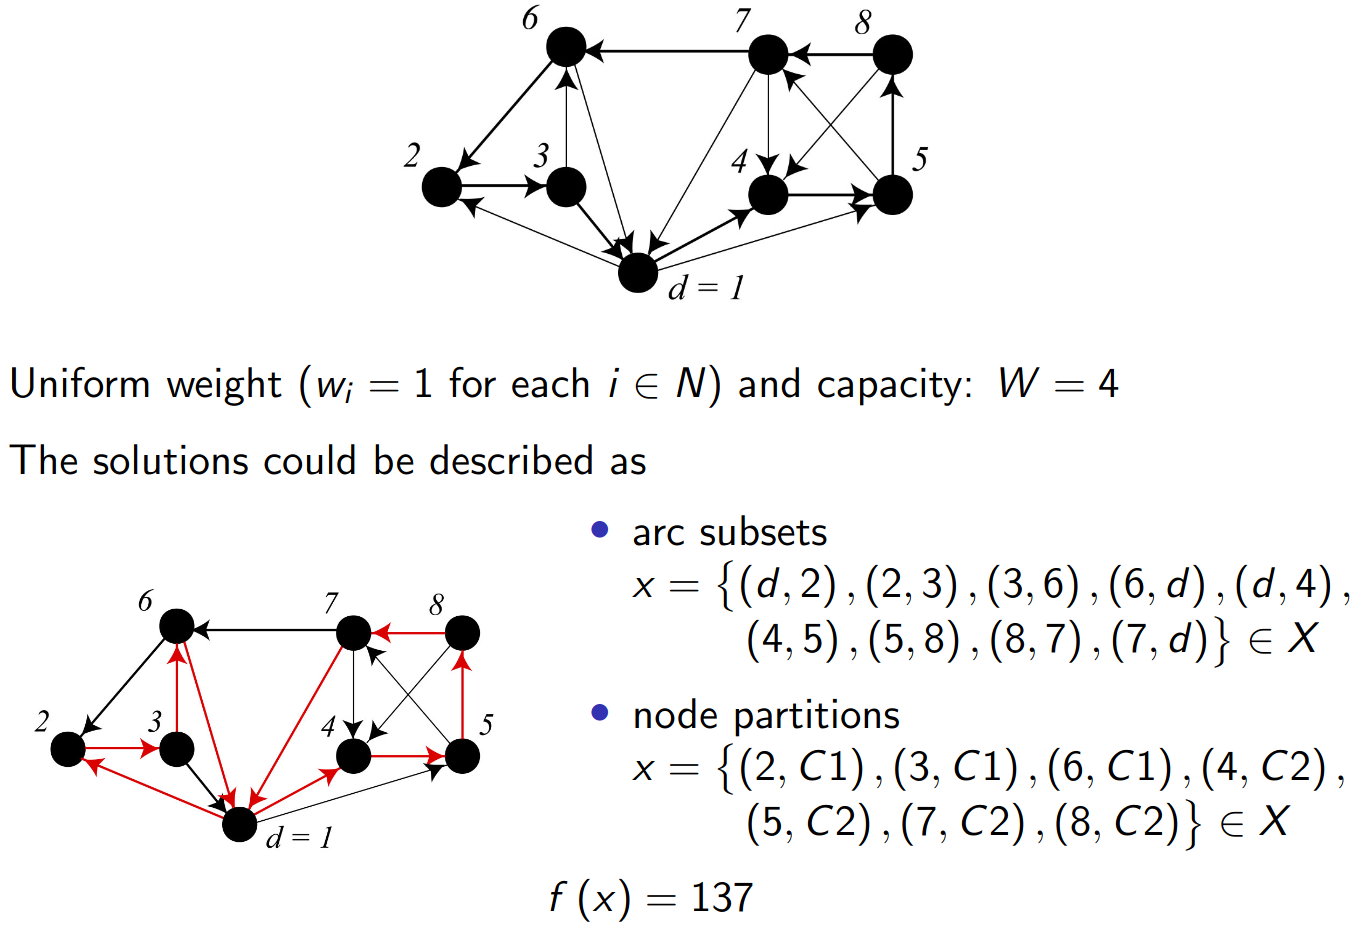
\includegraphics[width=0.9\columnwidth]{img/VRP1}
	\end{center}
	
	\newpage
	
	\subsection*{Interlude 6: Combining alternative representations}
	\addcontentsline{toc}{subsection}{Interlude 6: Combining alternative representations}
	The \textbf{CMSTP} and the \textbf{VRP} share an interesting complication: \textbf{different definitions of the ground set} $B$ are possible and natural
	\begin{itemize}
		\item the description as a \textbf{set of edges/arcs} looks preferable to \textbf{manage the objective}
		\item the description as a \textbf{set of pairs (vertex,tree)/(node,circuit)} looks better to \textbf{generate optimal solutions and to deal with feasibility}
	\end{itemize}
	
	Which description should be adopted?
	\begin{itemize}
		\item the one that makes easier the most frequent operations
		\item both, if they are used much more frequently than updated, so that the burden of keeping them up-to-date and consistent is acceptable
	\end{itemize}
	
	% End of L2
	
	\newpage
	
	\section{Computational Complexity}
	\paragraph{Problems:} informally, a problem is a \textbf{question} on a \textbf{system} of \textbf{mathematical objects}. The same question can often be asked on many similar systems
	\begin{itemize}
		\item an \textbf{instance} $i \in I$ is each specific system concerned by the question 
		\item a \textbf{solution} $s \in S$ is an answer corresponding to one of the instances
	\end{itemize}
	Formally, a problem is the f\textbf{unction which relates instances and solutions}
	$$ P : \, I \rightarrow S $$
	Defining a function doesn't mean knowing how to compute it.\\
	
	\paragraph{Algorithms:} an algorithm is a \textbf{formal procedure}, composed by \textbf{elementary steps}, in \textbf{finite sequence}, each determined by an input and by the results of the previous steps.\\
	
	An algorithm for a \textbf{problem} $P$ is an algorithm which, given in \textbf{input} $i \in I$, returns in \textbf{output} $S_i \in S$
	$$ A : \, \rightarrow S $$
	
	An algorithm \textbf{defines a function} plus the \textbf{way to compute} it; it can be
	\begin{itemize}
		\item \textbf{exact} if its associated function coincides with the problem
		\item \textbf{heuristic} otherwise
	\end{itemize}
	A heuristic algorithm is \textbf{useful} if it is
	\begin{enumerate}
		\item \textbf{efficient:} it "costs" much less than an exact algorithm
		\item \textbf{effective:} it "frequently" provides a solution "close" to the right one
	\end{enumerate}
	
	\newpage
	
	\subsection{Cost of an Algorithm}
	The "cost" of an algorithm denotes the \textbf{computational cost} of running it: 
	\begin{itemize}
		\item \textbf{space} occupied in memory
		\item \textbf{time} required to terminate
	\end{itemize}
	The \textbf{time} is usually considered more important, since: 
	\begin{itemize}
		\item space is \textbf{renewable}, can be reused, time isn't 
		\item using \textbf{space} always \textbf{requires time}
		\item usage of space is usually \textbf{easier} to \textbf{distribute} (among machines)
	\end{itemize}
	Space and time are \textbf{partly interchangeable}, it's possible to reduce use of one by increasing the other.\\
	
	Physical time is dependent on too many unreliable factors, and the measure of \textbf{computational time} should be 
	\begin{itemize}
		\item \textbf{unrelated to technology}, i.e. the same for different machines
		\item \textbf{concise}, summarized in a simple symbolic expression
		\item \textbf{ordinal}, sufficient to compare different algorithms
	\end{itemize}
	
	\newpage
	
	\subsection{Worst-case asymptotic time complexity}
	The Worst-case asymptotic time complexity provides such a measure through the passages of:
	\begin{enumerate}
		\item define the \textbf{time} $T$ as the \textbf{number of elementary operations} performed (independent from the specific machine)
		\item define the \textbf{size of an instance} as a suitable value $n$ (e.g. the number of elements in the ground set)
		\item find the \textbf{worst-case}, the maximum of $T$ \textbf{on all instances} of size $n$
		$$ T(n) = \max_{i \in I_n} T(i) \;\;\;\;\; n \in \mathbb{N} $$
		Now time complexity is a function $T : \, \mathbb{N} \rightarrow \mathbb{N}$.
		\item \textbf{approximate} $T(n)$ from above/below \textbf{with a simpler function} $f(n)$, considering only their \textbf{asymptotic behavior} (for $n \rightarrow +\infty$, we want an efficient algorithm on instances of large sizes)
		\item collect the function in \textbf{classes} with the \textbf{same approximating functions}
	\end{enumerate}
	
	\paragraph{$\Theta$ functional spaces:}
	$$ T(n) \in \Theta(f(n))$$
	Represents the \textbf{tight bound} of a function's growth rate, $T(n)$ must be "enclosed" between $c_1 f(n)$ and $c_2 f(n)$, from a "large" value of $n$, i.e. it's valid from a point $n_0$ forward.\\
	Asymptotically, $f (n)$ \textbf{estimates} $T (n)$ up to a multiplying factor.
	
	\paragraph{$O$ functional spaces:}
	$$ T(n) \in O(f(n))$$
	Represents the \textbf{upper bound} of a function's growth rate, $c \cdot f(n)$ "dominates" $T(n)$, from a point $n_0$ forward. \\
	Asymptotically, $f (n)$ \textbf{overestimates} $T (n)$ up to a multiplying factor.
	
	\paragraph{$\Omega$ functional spaces:}
	$$ T(n) \in \Omega(f(n))$$
	Represents the \textbf{lower bound} of a function's growth rate, $T(n)$ dominates $\Omega(n)$ from a point $n_0$ forward. \\
	Asymptotically, $f (n)$ \textbf{underestimates} $T (n)$ up to a multiplying factor.
	
	\newpage
	
	\subsubsection{The exhaustive algorithm}
	Within CO problems. Define the \textbf{size} of an instance as the \textbf{cardinality} of the \textbf{ground set}
	$$ n = |B| $$
	The exhaustive algorithm
	\begin{itemize}
		\item considers \textbf{each} and every \textbf{subset} $x \subseteq B$, that is each $x \in 2^{|B|}$
		\item test its \textbf{feasibility} ($x \in X$) in time $\alpha (n)$
		\item if positive, \textbf{evaluates} the \textbf{objective} $f(x)$ in time $\beta(n)$
		\item \textbf{updates} the best value found so far, if needed
	\end{itemize}
	The \textbf{time complexity} becomes
	$$ T(n) \in \Theta \left(2^n \left(\alpha (n) + \beta (n)\right)\right) $$
	This is \textbf{at least exponential}, even if $\alpha (n)$ and $\beta(n)$ are small polynomials (which is often the case).\\
	
	The exhaustive algorithm is impractical most of the time.
	
	\subsubsection{Polynomial and exponential complexity}
	In CO, the main \textbf{distinction} is between: 
	\begin{itemize}
		\item \textbf{polynomial complexity:} $T(n) \in O (n^d)$ for a constant $d > 0$
		\item \textbf{exponential complexity:} $T(n) \in \Omega(d^n)$ for a constant $d > 1$
	\end{itemize}
	The \textbf{first} family includes \textbf{efficient} algorithms, the \textbf{second} \textbf{inefficient} ones.\\
	
	In general, the \textbf{heuristic} algorithms are \textbf{polynomial} algorithms for problems whose known \textbf{exact} algorithms are all \textbf{exponential}.\\
	
	\newpage
	
	\subsection{Problem transformations and reductions}
	Problems can be \textbf{transformed} into other problems (\hyperref[I5]{Interlude 5}). A \textbf{relation} among problems allows to design algorithms: 
	\begin{itemize}
		\item by \textbf{transformation}: 
		\begin{enumerate}
			\item given $I_P$ (instance of $P$) \textbf{build} $I_Q$
			\item given $I_Q$, \textbf{apply} $A_Q$ to \textbf{obtain} $S_Q$ (solution of $I_Q$)
			\item given $S_Q$, \textbf{build} $S_P$
		\end{enumerate}
		\item by \textbf{reduction}: \textbf{repeat} the transformation, correcting $I_Q$ based on the \textbf{solutions obtained}; iterate the process
	\end{itemize}
	
	If $A_Q$ is exact/heuristic, $A_P$ is exact/heuristic.\\
	
	The two algorithms often have a \textbf{similar complexity}, if $A_Q$ is polynomial/exponential and
	\begin{itemize}
		\item building $I_Q$ takes polynomial time
		\item the number of iterations is polynomial
		\item building $S_P$ takes polynomial time
	\end{itemize}
	then $A_P$ is polynomial/exponential.\\
	
	\newpage
	
	\subsection{Beyond the worst-case complexity}
	The worst-case complexity \textbf{cancels} all information on the \textbf{easier instances} (maybe i just need to use easy instances) and gives a rough \textbf{overestimate} of the computational time, in some (rare) case useless.\\
	
	What if the \textbf{hard} instances are \textbf{rare} in practice? To \textbf{compensate} one can investigate: 
	\begin{itemize}
		\item \textbf{parameterized complexity}, that is introduce some \textbf{other relevant parameter} $k$ (besides the size $n$) and express the \textbf{time as} $T(n,k)$
		\item \textbf{average-case complexity}, that is assume a \textbf{probability distribution} on $I$ and express the \textbf{time} as the \textbf{expected value}
		$$ T(n) = E \left[T(i) | i \in I_n \right] $$
	\end{itemize}
	
	\subsubsection{Parameterized complexity}
	Some algorithms are \textbf{exponential} in $k$ an \textbf{polynomial} in $n$ and thus: 
	\begin{itemize}
		\item \textbf{efficient} on instances with \textbf{low} $k$
		\item \textbf{inefficient} on instances with \textbf{large} $k$
	\end{itemize}
	\begin{center}
		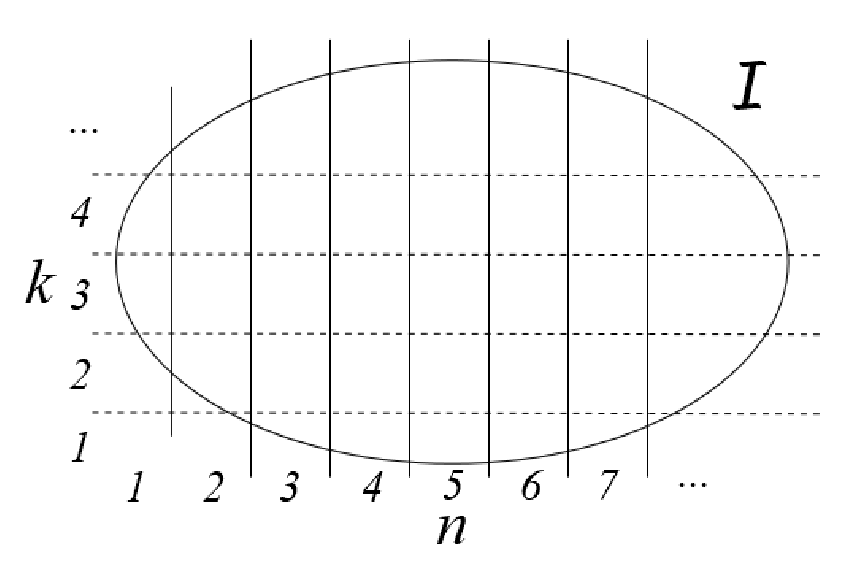
\includegraphics[width=0.5\columnwidth]{img/PC1}
	\end{center}
	
	\newpage
	
	\paragraph{Nature of $k$:} it could be part of the \textbf{input}: 
	\begin{itemize}
		\item a \textbf{numerical constant} (e.g. the capacity of the KP)
		\item the \textbf{maximum number of literals} per formula in logic function problems
		\item the \textbf{number on nonzero elements} in numerical matrix problems
		\item the \textbf{maximum degree}, \textbf{the diameter}, etc... in graph problems
	\end{itemize}
	one knows \textit{a priori} whether the algorithm is efficient on a given instance.\\
	
	If the additional parameter $k$ is part of the \textbf{solution}: 
	\begin{itemize}
		\item the \textbf{cardinality} of the solution
	\end{itemize}
	one will only find out \textit{a posteriori} (but an estimate \textit{a priori} could be available).\\
	
	\paragraph{Example: the VCP;} \textbf{Exhaustive algorithm:} for each of the $2^n$ subsets of vertices, test if it covers all edges, compute its cardinality and keep the smallest one
	$$ T(n,m) \in \Theta \left(2^n (m+n)\right) $$
	If we already know that there's a solution with $f(x) = |x| = k+1$, we can look for a solution of $k$ vertices, decreasing $k$ progressively; if we can't find it we already have the optimal solution.\\
	
	\textbf{Naive algorithm:} for each subset of $k$ vertices, test if it covers all edges
	$$ T(n,m,k) \in \Theta \left(n^k m\right) $$
	for a fixed $k$, this algorithm is polynomial (but in general very slow).\\
	
	\newpage
	
	\textbf{Bounded tree search:} a better algorithm can be based on the following useful property
	$$ x \cap (u,v) \neq \emptyset \text{ for all } x \in X, \, (u,v) \in E $$
	Any feasible solution \textbf{includes} at least one \textbf{extreme vertex} for each edge.\\
	Choose any edge (there can be "good" and "bad" edges), only one must be in the solution.\\
	
	BTS algorithm to find $x$ with $|x| \leq k$:
	\begin{enumerate}
		\item choose \textbf{any} $(u,v)$: either $u \in x$ or $u \notin x$ and $v \in x$ (there must be only one in the solution)
		\item for each open case, \textbf{remove} the \textbf{vertices} of $x$ and the \textbf{edges they cover}
		$$ V := V \setminus x \;\;\;\;\; E := E \setminus \left\{e \in E: \, e \cap x \neq \emptyset \right\}$$
		The edges covered by vertices in $x$ are no longer constraining
		\item if $|x| \leq k$ and $E = \emptyset$, $x$ is the \textbf{required solution}; if the partial solution has $k$ elements (or less) and there are no more edges to cover then it's not a partial solution, it's a feasible one
		\item if $|x| \leq k$ and $E \neq \emptyset$, there is \textbf{no solution}
		\item otherwise go to step 1
	\end{enumerate}
	The \textbf{complexity} is $T(n,m,k) \in \Theta(2^k m)$, polynomial in $n$ ($m < n^2$). \\
	For $n>>2$, this algorithm is much more efficient than the naive one.\\
	
	\newpage
	
	\subsubsection{Kernelization (or "problem reduction")}
	Kernelization \textbf{transforms} all \textbf{instances} of $P$ into \textbf{simpler} instances of $P$ (also known as "problem reduction"), instead of instances of another problem $Q$.\\
	
	Quite often, in fact, useful \textbf{properties} allow to \textbf{prove that}
	\begin{itemize}
		\item there exists an optimal solution (not every optimal solution, but at least one) \textbf{not including} certain elements of $B \implies$ such elements can be \textbf{removed}
		\item there exists an optimal solution \textbf{including} certain elements of $B \implies$ such elements can be set \textbf{apart and added later}
	\end{itemize}
	In short, remove elements of $B$ without affecting the solution.\\
	
	Possible useful \textbf{outcomes} are
	\begin{itemize}
		\item an \textbf{exact} algorithm \textbf{polynomial} in $n$ (the problem becomes simpler, parameterized complexity)
		\item \textbf{faster} exact and heuristic algorithms (the instance is smaller so it's faster and usually better since the smaller problem is less "confusing")
		\item \textbf{better} heuristic \textbf{solutions}
		\item \textbf{heuristic kernelization:} apply \textbf{relaxed conditions} sacrificing optimality (risk losing the optimal solution but simplify the problem)
	\end{itemize}
	
	\newpage
	
	\paragraph{Kernelization of VCP:} if $\delta_v \geq k+1$ (the degree of $v$, number of vertices), vertex $v$ belongs to any feasible solution of value $\leq k$ (you need to cover a lot of edges, this covers a lot of edges; by contradiction, you can't cover $k+1$ edges with less than this single vertex).\\
	
	Kernelization algorithm to \textbf{keep} only \textbf{vertices of solution} $x$ with $|x| \leq k$
	\begin{itemize}
		\item start at \textbf{step} $t = 0$ with $k_0 = k$ and an \textbf{empty} vertex \textbf{subset} $x_t := \emptyset$
		\item \textbf{set} $t = t + 1$ and \textbf{add} to the solution the \textbf{vertices of degree} $\geq k_t + 1$
		$$ \delta_v \geq k+1 \implies x_t := x_{t-1} \cup \left\{v\right\} $$
		\item \textbf{update} $k_t := k_0 − |x_t|$
		\item \textbf{remove} the \textbf{vertices} of \textbf{zero degree}, those \textbf{of} $x$ and the \textbf{covered edges}
		$$ V := \left\{v \in V : \, \delta_v > 0\right\} \setminus x_t \;\;\;\;\; E := \left\{e \in E : \, e \cap x_t = \emptyset \right\} $$
		\item if $|E| > k_t^2$ there is \textbf{no feasible solution} ($k_t$ vertices are not enough)
		\item if $|E| \leq k_t^2 \implies |V| \leq 2k_t^2$; \textbf{apply} the \textbf{exhaustive} algorithm
	\end{itemize}
	The \textbf{complexity} is $T(n,k) \in \Theta \left(n + m + 2^{2k^2}k^2 \right)$ (the last part is the one of the exhaustive algorithm, good if $k$ is small).\\
	
	\textbf{Essentially:} it chooses the nodes with the most edges connected to them, removes them (and the nodes left with no edges), decreases the number of edges "required" to be "chosen" and starts again.\\
	
	\newpage
	
	\subsubsection{Average-case complexity}
	Some algorithms are inefficient only on a few instances (see simplex algorithm for Linear Programming).\\
	
	\textbf{Idea:} define time as the \textbf{expected value} of $T(i)$ on $I_n$ for each $n \in \mathbb{N}$
	$$ T(n) = E \left[T(i) | i \in I_n \right]$$
	\textbf{Theoretical} studies can define a \textbf{probabilistic model} of the problem, that is a probability \textbf{distribution} on $I_n$ for each $n \in \mathbb{N}$ (probability of each instance, typically quite simple, could be equiprobability) and \textbf{compute} the \textbf{expected value} of $T(I)$.\\
	
	\textbf{Empirical} studies
	\begin{itemize}
		\item build a \textbf{simulation model} of the problem, that is a probability distribution on $I_n$ for each $n \in \mathbb{N}$, let it be theoretical or empirical (drawn from real-world data) 
		\item build a \textbf{benchmark} of \textbf{random} instances according to the \textbf{distribution}
		\item apply the algorithm and \textbf{measure} the \textbf{time} required
	\end{itemize}
	
	\paragraph{Probabilistic models for numerical matrices:} Binary random matrix with a given size ($m$ rows and $n$ columns), some models are: 
	\begin{enumerate}
		\item \textbf{equiprobability:} list all $2^{mn}$ binary matrices and select one of the matrices with uniform probability
		\item \textbf{uniform probability:} set each cell to $1$ with a given probability $p$
		$$ Pr[a_{ij} = 1] = p \;\;\;\;\; (i = 1, \, ... \, , m; \, j = 1, \, ... \, , n) $$
		If $p = 0.5$, it coincides with the equiprobability model, for other values some instances are more likely than others
		\item \textbf{fixed density:} extract $\delta mn$ (obviously $0 < \delta < 1$) cells out of $mn$ with uniform probability and set them to $1$.\\
		If $\delta = p$, it resembles the uniform probability model, but some instances cannot be generated
	\end{enumerate}
	
	\newpage
	
	\paragraph{Probabilistic models for graph:} Random graph with a given number of vertices $n$, some models are: 
	\begin{enumerate}
		\item \textbf{equiprobability:} list all $2^{\frac{n(n-1)}{2}}$ graphs and select one of the graphs with uniform probability
		\item \textbf{Gilbert’s model}, or \textbf{uniform probability} $G (n, p)$:
		$$ Pr  \left[(i,j) \in E \right] = p \;\;\;\;\; \left(i \in V , \, j \in V \setminus \left\{i\right\}\right)$$
		All graphs with the same number of edges $m$ have the same probability $p^m (1 − p)^{\frac{n(n-1)}{2} - m}$ (different for each $m$).\\
		If $p = 0.5$, it coincides with the equiprobability model
		\item \textbf{Erd\H{o}s-R\'enyi model} $G (n, m)$: extract $m$ unordered vertex pairs out of $\frac{n(n-1)}{2}$ with uniform probability and create an edge for each one
		If $\frac{2m}{n(n-1)} = p$, it resembles the uniform probability model, but some instances cannot be generated
	\end{enumerate}
	
	\paragraph{Probabilistic models for logic functions:} Random CNF with a given number of variables $n$ and a given number of literals $k$ for each logic formula
	\begin{enumerate}
		\item \textbf{fixed-probability ensemble:} list all $\left(\begin{array}{c} n \\ k\end{array}\right) 2^k$ formulae of $k$ distinct and consistent literals and add each one to the CNF with probability $p$
		\item \textbf{fixed-size ensemble:} build $m$ formulae, adding to each one $k$ distinct and consistent literals, extracted with uniform probability.\\
		If $p = \frac{m}{\left(\begin{array}{c} n \\ k\end{array}\right) 2^k}$, it resembles the fixed-probability model, but some instances cannot be generated
	\end{enumerate}
	
	\newpage
	
	\subsubsection{Phase transitions}
	Different values of the (deterministic or probabilistic) \textbf{parameters} correspond to \textbf{different regions} of the \textbf{instance} set.\\
	If you introduce parameters, different regions of the instance set are obtained.\\
	
	For \textbf{graphs}
	\begin{itemize}
		\item $m = 0$ and $p = 0$ correspond to \textbf{empty graphs}
		\item $m = \frac{n(n−1)}{2}$ and $p = 1$ correspond to \textbf{complete graphs }
		\item intermediate values correspond to graphs of \textbf{intermediate density} (deterministically for $m$, probabilistically for $p$)
	\end{itemize}
	You can expect the algorithm to perform differently on different regions.\\
	
	For many problems the \textbf{performance} of algorithms is strongly \textbf{different in different regions} concerning
	\begin{itemize}
		\item the \textbf{computational time} (for exact and heuristic algorithms)
		\item the \textbf{quality of the solution} (for heuristic algorithms)
	\end{itemize}
	Often, the performance \textbf{variation} takes place \textbf{abruptly} in \textbf{small regions} of the parameter space, as in phase transitions of physical systems (e.g. ice to water happens in a restricted zone).\\
	This is useful to predict the behavior of an algorithm on a given instance.\\
	
	\newpage
	
	\paragraph{Phase transitions for 3-SAT and Max-3-SAT:} Given a CNF on $n$ variables, with logic formulae containing $3$ literals
	\begin{itemize}
		\item \textbf{3-SAT:} is there a truth assignment satisfying all formulae?
		\item \textbf{Max-3-SAT:} what is the maximum number of satisfiable formulae?
	\end{itemize}
	As the formulae/variables ratio, $\alpha = m/n$, increases
	\begin{itemize}
		\item \textbf{satisfiable instances decrease} from nearly all (many variables for few formulae) to nearly none (few variables for many formulae)
		\item the \textbf{computing time} first \textbf{sharply increases}, then \textbf{decreases} for SAT, increases further for Max-SAT (using a well-known exact algorithm)
	\end{itemize}
	\begin{center}
		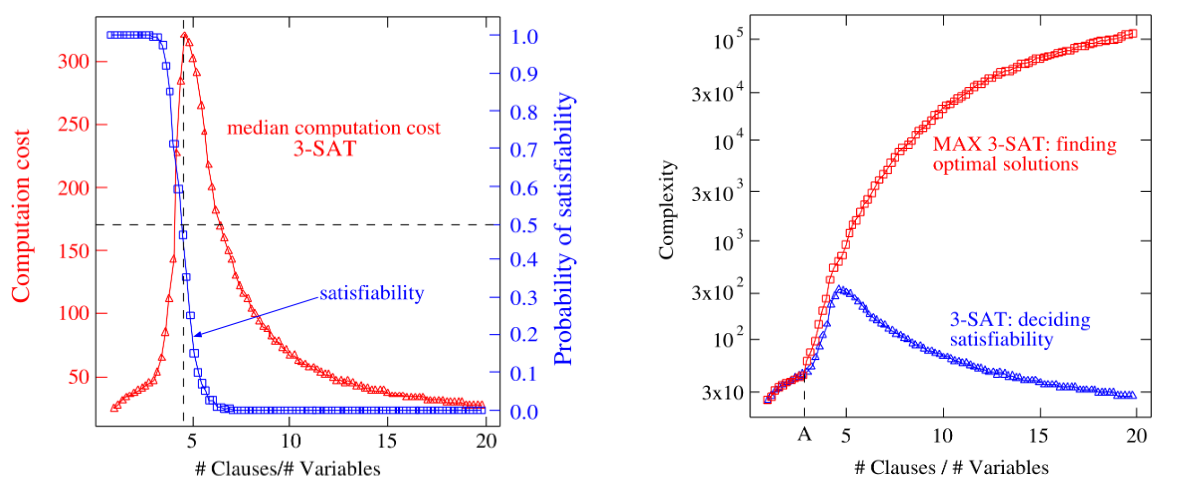
\includegraphics[width=\columnwidth]{img/PhaseT1}
	\end{center}
	The blue profile in the first graph (3-SAT) shows the number of instances that can be satisfied for a certain number of clauses/variables. The red shows the computational time (on a specific algorithm, but many have the same basic ideas), which starts small, gets big and then decreases (as stated before), there's a range, where the lines meet, which makes it hard to prove the satisfiability of the clauses.\\
	
	In second graph (Max-3-SAT) the blue profile shows the complexity of deciding satisfiability (same as red in the first graph, re-scaled), the red one shows the complexity of finding optimal solutions, which only increases.\\
	
	As $n \rightarrow + \infty$, the transition \textbf{concentrates} around $\alpha_c \approx 4.26$.\\
	
	\newpage
	
	\paragraph{Phase transition for the VCP:} The \textbf{VCP} exhibits a \textbf{similar phase transition} as $|x|/|V|$ increases, the computational time first explodes, then drops, as $n \rightarrow +\infty$ \textbf{concentrates} around a critical value.
	\begin{center}
		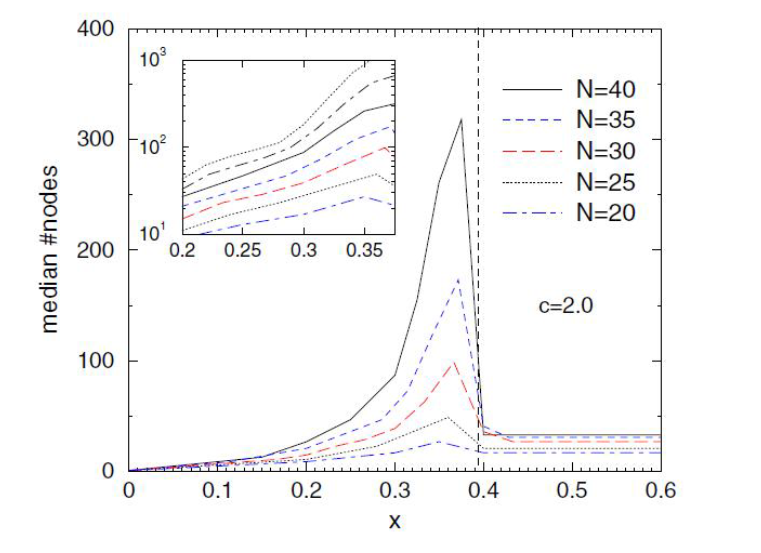
\includegraphics[width=0.7\columnwidth]{img/PhaseT2}
	\end{center}
	When $|x|/|V|$ is small some vertices are clearly necessary, when it's large many vertices are clearly necessary; in both cases, problem solved.\\
	
	\vfill 
	
	\subsection*{Computational cost of heuristic algorithms}
	\addcontentsline{toc}{subsection}{Computational cost of heuristic algorithms}
	The \textbf{time complexity} of a heuristic algorithm is usually
	\begin{itemize}
		\item \textbf{strictly polynomial} (with low exponents)
		\item fairly \textbf{robust} with respect \textbf{to secondary parameters}
	\end{itemize}
	Therefore, the worst-case estimation is also good on average.\\
	
	\textbf{Metaheuristics} use random steps or memory
	\begin{itemize}
		\item the \textbf{complexity} is \textbf{well defined} for \textbf{single components} of the algorithm
		\item the \textbf{overall complexity} is \textbf{not clearly defined}
		\begin{itemize}
			\item in \textbf{theory}, it could extend \textbf{indefinitely} (but the pseudo-random number generator or the memory configurations would yield an infinite loop)
			\item in \textbf{practice}, it is defined by a \textbf{condition} imposed by the \textbf{user} 
		\end{itemize}
	\end{itemize}
	
	% End of L3
	
	\newpage
	
	\section{Effectiveness of a heuristic algorithm}
	As stated before, a heuristic algorithm is \textbf{useful} if it is: 
	\begin{itemize}
		\item \textbf{efficient:} it "costs" much less than an exact algorithm
		\item \textbf{effective:} it "frequently" returns a solution "close to" an exact one
	\end{itemize}
	The \textbf{effectiveness} can be described in terms of: 
	\begin{itemize}
		\item \textbf{closeness} of the solution to the \textbf{optimal one} 
		\item \textbf{frequency} of \textbf{hitting optimal} or nearly optimal \textbf{solutions}
	\end{itemize}
	These features can be combined into a \textbf{frequency distribution} of \textbf{solutions} more or less close to the \textbf{optimum}.\\
	
	The effectiveness can be \textbf{investigated} with a: 
	\begin{itemize}
		\item \textbf{theoretical analysis} (\textit{a priori}), \textbf{proving} that the \textbf{algorithm finds} always or with a given frequency \textbf{solutions} with a given guarantee of quality; this is done by looking at the structure of the algorithm
		\item \textbf{experimental analysis} (\textit{a posteriori}), \textbf{measuring} the \textbf{performance} of the algorithm on sampled \textbf{benchmark instances} to show that it occurs
	\end{itemize}
	
	\newpage
	
	\subsection{Distance} 
	We need to define a distance to be able to \textbf{measure} the \textbf{effectiveness} of algorithms.\\
	The effectiveness of a heuristic optimization algorithm $A$ is measured by the \textbf{difference} between the heuristic \textbf{value} $f_A (i)$ and the \textbf{optimum} $f^\ast (i)$
	\begin{itemize}
		\item \textbf{Absolute difference}
		$$ \tilde{\delta}_A (i) = |f_A(I) - f^\ast (i)| \geq 0 $$
		used rarely and only when the objective is a pure number. This yields a small error an small instances and big numbers on big instances so it could be not significant.\\
		\item \textbf{Relative difference}
		$$ \delta_A (i) = \frac{|f_A (i) - f^\ast (i)|}{f^\ast (i)} \geq 0$$
		frequent in experimental analysis (usually as a percent ratio).\\
		\item \textbf{Approximation ratio}
		$$ \rho_A (i) = \max \left[\frac{f_A(i)}{f^\ast(i)}, \, \frac{f^\ast (i)}{f_A (i)}\right] \geq 1 $$
		frequent in theoretical analysis: the first form is used for minimization problems, the second one for maximization ones. The formula is done this way to represent both problems with a single expression.\\
	\end{itemize}
	
	\newpage
	
	\subsection{Theoretical analysis}
	\subsubsection{Worst case}
	To obtain a compact measure, independent of $i$, find the worst case.\\
	
	The \textbf{difference} between $f_A (i)$ and $f^\ast(i)$ is in general unlimited, but for some algorithms it is \textbf{limited}:
	\begin{itemize}
		\item \textbf{absolute approximation:}
		$$ \exists \tilde{\alpha}_A \in \mathbb{N} : \, \tilde{\delta}_A (i) \leq \tilde{\alpha}_A \text{ for each } i \in I $$
		A (rare) example is Vizing's algorithm for Edge Coloring ($\tilde{\alpha}_A = 1$). The result will never be worse than the optimum by more than a fixed amount.
		\item \textbf{relative approximation:}
		$$ \exists \alpha_A \in \mathbb{R}^+ : \, \rho_A (i) \leq \alpha_A \text{ for each } i \in I $$
		the ratio of the heuristic solution and the optimal one is not larger than a constant $\alpha$ (must be $\geq 1$).
	\end{itemize}
	Factor $\alpha_A$ ($\tilde{\alpha}_A$) is the relative (absolute) \textbf{approximation guarantee}.\\
	
	For other algorithms, the guarantee \textbf{depends} on the \textbf{instance size}
	$$ \rho_A (i) \leq \alpha_A (n) \text{ for each } i \in I_n, \, n \in \mathbb{N} $$
	The approximation guarantee can change in relation to the instance size, (twice the size, twice as "less optimum" for example) so the guarantee can be expressed via a function.\\
	
	Effectiveness can be \textbf{independent from size} (contrary to efficiency).\\
	
	\newpage
	
	\paragraph{Achieving an approximation guarantee:} For a minimization problem, the aim is to \textbf{prove} that
	$$ \exists \alpha_A \in \mathbb{R} : \, f_A (i) \leq \alpha_A f^\ast (i) \text{ for each } i \in I $$
	We need to prove that $A$ gives a \textbf{heuristic value} $f_A$ on instance $i$ that is \textbf{not larger} than a certain constant $\alpha$ times the optimal.\\
	
	To \textbf{prove} it
	\begin{enumerate}
		\item find a way to build an \textbf{underestimate} $LB(i)$
		$$ LB(i) \leq f^\ast (i) \;\;\;\; i \in I $$
		for any instance, the underestimate must be smaller or equal to the optimum
		\item find a way to build an \textbf{overestimate} $UB(i)$, related to $LB(i)$ by a \textbf{coefficient} $\alpha_A$
		$$ UB(i) = \alpha_A LB(i) \;\;\;\; i \in I $$
		we found a lower bound, now we need an estimate for the upper bound, which will be at most $\alpha$ times the lower bound
		\item find an \textbf{algorithm} $A$ whose solution is not worse than $UB(i)$
		$$ f_A (i) \leq UB(i) \;\;\;\; i \in I $$
	\end{enumerate}
	Then $f_A (i) \leq UB(i) = \alpha LB(i) \leq \alpha f^\ast (i)$, for each $i \in I$, we \textbf{proved} that
	$$ f_A (i) \leq \alpha_A f^\ast (i) \text{ for each } i \in I $$
	our algorithm is at least $\alpha$ \textbf{times} the optimum.\\
	
	\newpage
	
	\paragraph{A 2-approximated algorithm for the VCP:} Given an \textbf{undirected graph} $G = (V , E )$ find the \textbf{minimum cardinality vertex subset} such that each \textbf{edge} of graph is \textbf{incident} to it.\\
	
	A \textbf{matching} is a set of nonadjacent edges (they're connected to different vertices, they don't have common vertices).\\
	\textbf{Maximal matching} is a matching such that any other edge of the graph is adjacent to one of its edges (it cannot be enlarged, any other edge is adjacent to one of the matching).\\
	
	\textbf{Matching} algorithm:
	\begin{enumerate}
		\item Build a \textbf{maximal matching} $M \subseteq E$ scanning the edges of $E$ and including in $M$ those not adjacent to $M$ (now every edge of $E \setminus M$ is adjacent to an edge of $M$)
		\item The \textbf{set of extreme vertices} of the matching edges is a VCP \textbf{solution}
		$$ x_A := \bigcup_{(u,v) \in M} \left\{u,v\right\}$$
		and it can be improved removing the redundant vertices, as this can leave some unnecessary ones.
	\end{enumerate}
	It basically takes all the nonadjacent edges and considers the relative vertices.\\
	
	\newpage
	
	\textbf{Example:}
	\begin{center}
		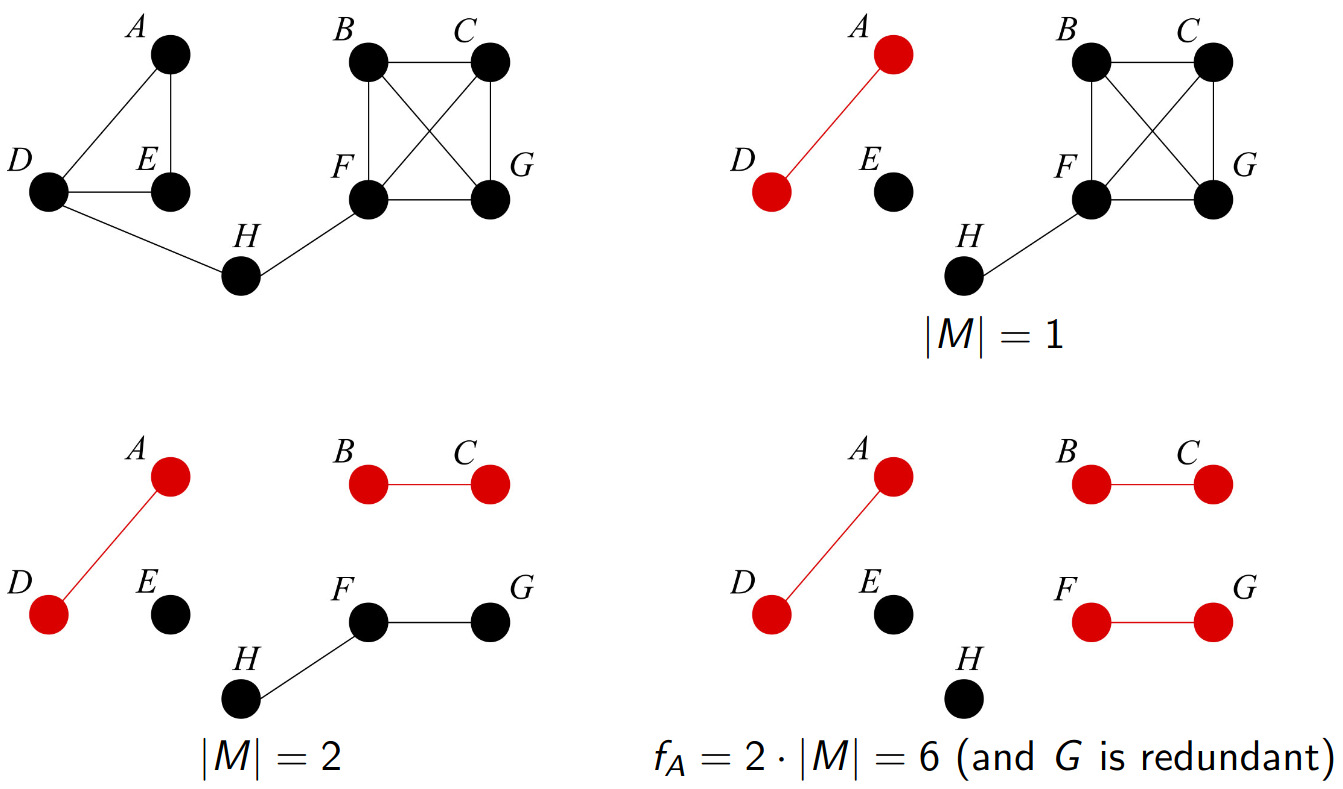
\includegraphics[width=\columnwidth]{img/VCP2Approx}
	\end{center}
	
	\textbf{Proof:} The matching algorithm is 2-approximated
	\begin{enumerate}
		\item The \textbf{cardinality} of matching $M$ is an \textbf{underestimate} $LB (i )$
		\begin{itemize}
			\item the cardinality of an \textbf{optimal covering} for any subset of edges $E' \subseteq E$ does not exceed that of an optimal covering for $E$
			$$ |x_{E'}^\ast| \leq |x_E^\ast|$$
			(it costs more to cover all edges than only the matching, obviously since the matching is smaller)
			\item the \textbf{optimal covering} of a \textbf{matching} $M$ has \textbf{cardinality} $|M|$ (each edge of the matching requires exactly one different vertex, we're essentially considering half the vertices in the matching, which can cover all the relative edges)
		\end{itemize}
		\item \textbf{Including both} the \textbf{extremes} of each edge of the matching yields
		\begin{itemize}
			\item an \textbf{overestimate} (it covers both the matching and all adjacent edges, i.e. a VCP solution for every maximal matching)
			\item of \textbf{value} $UB (i ) = 2LB (i )$ (two different vertices for each edge, double the cardinality which is our possible $LB (i)$)
		\end{itemize}
		\item The \textbf{matching algorithm} returns \textbf{solutions} of value $f_A (i ) \leq UB (i )$ (possibly removing redundant vertices)
	\end{enumerate}
	This \textbf{implies} $f_A (i ) \leq 2f^\ast (i )$ for each $i \in I$, since $\alpha_A = 2$.\\
	
	\textbf{And the bound is tight:} Since $\alpha_A$ \textbf{relates} $UB (i )$ and $LB (i )$, $f_A (i )$ and $f^\ast (i )$ could be closer.\\
	Actually, for many instances $\rho_A (i )$ is much better than $\alpha_A$.\\
	
	Are there instances $\overline{i}$ for which $f_A (\overline{i}) = \alpha_A f^\ast (\overline{i})$? How are they like? \\
	Our value $f_A(i)$ is \textbf{at most} $\alpha_A$ times the \textbf{optimum}, are there instances where our \textbf{solution} is  exactly $\alpha_A$ times the optimal?\\
	
	The study of these instances is useful to
	\begin{itemize}
		\item \textbf{evaluate} whether they are \textbf{rare or frequent}
		\item introduce \textbf{ad hoc modifications} to improve the algorithm
	\end{itemize}
	\begin{center}
		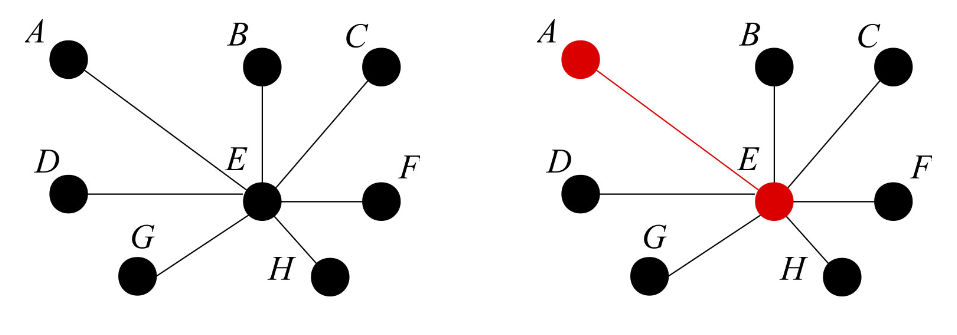
\includegraphics[width=0.8\columnwidth]{img/VCP2Approx2}
	\end{center}
	In this case our heuristic solution is exactly $\alpha_A$ (2) times the optimum, this is the worst case.\\
	
	In the literature the typical expression "and the bound is tight" introduces the description of instances exhibiting the worst case.\\
	If all worst cases are patched, the approximation guarantee improves.\\
	
	\newpage
	
	\paragraph{The TSP under the triangle inequality:} Consider the \textbf{TSP} with the additional (rather common) \textbf{assumptions} that
	\begin{itemize}
		\item graph $G = (N, A)$ is \textbf{complete}
		\item cost $c$ is \textbf{nonnegative}, \textbf{symmetric} and \textbf{satisfies} the \textbf{triangle inequality}
		$$ c_{ij} = c_{ji} \;\; \forall i,j \in N \;\; \text{ and } \;\; c_{ij} + c_{jk} \leq c_{ik} \;\; \forall i,j,k \in N $$
		i.e. the road works equally both ways and there can't be roads that connect $i$ and $j$ and subsequently $k$ shorter than the road $ik$ (the costs can form a triangle)
	\end{itemize}
	
	\textbf{Double-tree} algorithm
	\begin{enumerate}
		\item Consider the \textbf{complete undirected graph} corresponding to $G$
		\item Build a \textbf{minimum cost spanning tree} $T^\ast = (N, X^\ast)$
		\item Make a \textbf{pre-order visit} of $T^\ast$ and build two lists of arcs:
		\begin{enumerate}[label=\alph*.]
			\item $x'$ lists the arcs used \textbf{both} by the \textbf{visit} and the \textbf{backtracking}: this is a circuit visiting each node, possibly several times; exactly twice the cost of the original minimum spanning tree, it's visiting all the nodes
			\item $x$ lists the arcs linking the \textbf{nodes in pre-order ending with the first}: this is a circuit visiting each node exactly once; we use the triangle inequality to go directly across nodes, removing some backtracking and visiting each node only once
		\end{enumerate}
	\end{enumerate}
	
	Example:
	\begin{center}
		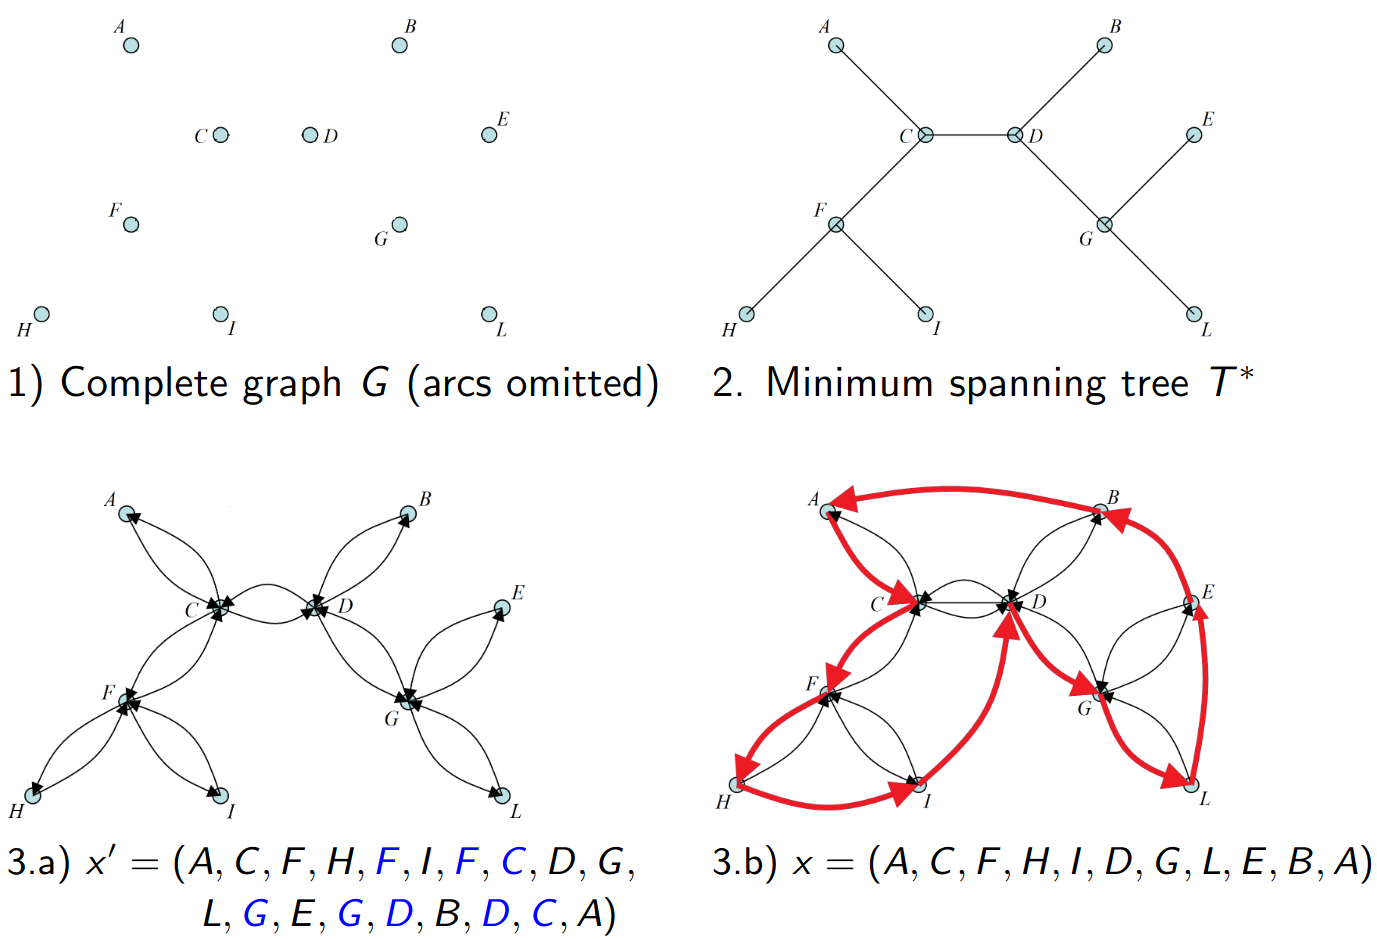
\includegraphics[width=0.8\columnwidth]{img/TSTTI1}
	\end{center}
	
	\newpage
	
	The cost of the hamiltonian circuit will be at most equal to twice the spanning tree, which is at most equal to the optimal hamiltonian circuit. The \textbf{cost} is at most \textbf{twice the optimum}. \\
	
	To do the last step you can just look at the path and skip already seen nodes, since it's a complete graph there will be a path to the next unseen node and, as stated by the triangle inequality, it will certainly be $\leq$ than before. \\
	
	This way the result is exactly an hamiltonian circuit, with a cost smaller than the double tree, which has a cost equal to twice the tree, which itself has a cost that smaller than the optimum.\\
	
	The double-tree algorithm is \textbf{2-approximated}:
	\begin{enumerate}
		\item the \textbf{cost} of the \textbf{minimum spanning tree} is an \textbf{underestimate} $LB (i )$
		\begin{itemize}
			\item \textbf{deleting} an \textbf{arc} from a Hamiltonian circuit yields a Hamiltonian \textbf{path} that is \textbf{cheaper}
			\item a \textbf{Hamiltonian path} is a \textbf{spanning tree} (usually not of minimum cost)
		\end{itemize}
		\item the \textbf{cost} of circuit $x'$ is
		\begin{itemize}
			\item an \textbf{overestimate} $UB (i )$ (it is a non-minimum Hamiltonian circuit)
			\item \textbf{equal} to $2LB (i )$ (two arcs correspond to each edge)
		\end{itemize}
		\item the \textbf{cost} of circuit $x$ is $f_A (i ) \leq UB (i )$ (a single direct arc replacing a sequence decreases the cost)
	\end{enumerate}
	This \textbf{implies} that $f_A (i ) \leq 2f^\ast (i )$ for each $i \in I$, so we get $\alpha_A = 2$.\\
	
	Notice: $x'$ is used in the approximation proof, but doesn't need to be computed.\\
	
	\newpage
	
	\paragraph{Inapproximability:} For an inapproximable problem, \textbf{approximated algorithms would be exact}.\\
	Consider this family of TSP instances on \textbf{complete graphs}:
	\begin{itemize}
		\item $c_{ij} = 0$ for $(i, j) \in A_0$
		\item $c_{ij} = 1$ for $(i, j) \in  (N \times N) \ A_0$ (the \textbf{triangle inequality is violated}, the earlier approximation can't be applied anymore)
	\end{itemize}
	Essentially, some arcs are $0$, some $1$, triangle inequality cannot hold.\\
	
	The \textbf{optimum} of any such instance $\overline{i}$ is:
	\begin{displaymath}
		\begin{cases}
			f^\ast (\overline{i}) = 0 & \text{ if } A_0 \text{ contains a hamiltonian circuit} \\
			f^\ast (\overline{i}) \geq 1 & \text{ otherwise}
		\end{cases}
	\end{displaymath}
	(in the latter case, the optimal solution contains at least an arc $\notin A_0$, i.e. an arc that costs $1$).\\
	
	Assume that a \textbf{polynomial algorithm} $A$ provides a \textbf{guarantee} $\alpha_A$
	$$ f^\ast (i) \leq f_A (i) \leq \alpha f^\ast (i) \;\; \forall i \in I $$
	Then $f^\ast (\overline{i}) = 0 \Leftrightarrow f_A (\overline{i}) = 0$.\\
	
	Whenever the subgraph $G (N, A_0)$ has a Hamiltonian circuit, our algorithm $A$ necessarily finds it, solving an NP-complete problem in polynomial time (P $=$ NP, unlikely as this is of the millennium problems (I think)).\\
	
	\newpage
	
	\paragraph{Approximation schemes:} For hard problems
	\begin{itemize}
		\item \textbf{exact} algorithms provide the \textbf{best} approximation \textbf{guarantee} ($\alpha_A = 1$, they are exact after all), but require \textbf{exponential time} $T_A$
		\item \textbf{approximated} algorithms provide a \textbf{worse guarantee} ($\alpha_A > 1$), but could require \textbf{polynomial time} $T_A$
	\end{itemize}
	
	Some problems admit a \textbf{family of algorithms} providing a whole \textbf{range of compromises} between \textbf{efficiency} ed \textbf{effectiveness}
	\begin{itemize}
		\item better and better approximation guarantees: $\alpha_{A_1} > \, ... \, > \alpha_{A_r}$
		\item worse and worse computational complexities: $T_{A_1} < \, ... \, < T_{A_r}$
	\end{itemize}
	We can have multiple algorithms with different guarantees.\\
	
	Approximation scheme is a parametric algorithm $A_\alpha$ allowing to choose $\alpha$ (Example: the KP).\\
	
	\newpage
	
	\subsubsection{Beyond the worst case}
	As usual, the worst-case approach is rough: some algorithms often have a good performance, though sometimes bad.\\
	
	The \textbf{alternative approaches} are similar to the ones used for complexity
	\begin{itemize}
		\item \textbf{parametrisation:} prove an \textbf{approximation guarantee} that \textbf{depends} on \textbf{other parameters} of the instances besides the size $n$
		\item \textbf{average-case:} assume a \textbf{probability distribution} on the \textbf{instances} and evaluate the \textbf{expected value} of the approximation factor; the probability affects only the approximation factor, which is reasonable to assume can vary among instances (the algorithm could have a bad performance only on rare instances)
	\end{itemize}
	
	but there is at least \textbf{another approach}: 
	\begin{itemize}
		\item \textbf{randomization:} the \textbf{operations} of the algorithm \textbf{depend} not only on the instance, but \textbf{also on pseudo-random numbers}, so that the \textbf{solution} becomes a \textbf{random variable} which can be investigated (the time complexity could also be random, but usually is not).\\ 
		Random numbers are used to make decisions inside the algorithm, running it several time provides different results, the distribution of such results can be studied, usually in relation to the random seed used for each specific iteration. \\
	\end{itemize}
	
	\newpage
	
	\subsubsection{Randomized approximation algorithms}
	For a randomised algorithm $A$, $f_A (i , \omega)$ and $\rho_A (i , \omega)$ are random variables depending on the pseudo-random number seed $\omega$.\\
	
	A randomised approximation algorithm has an approximation ratio whose expected value is limited by a constant
	$$ E \left[\rho_A (i, \omega)\right] \leq \alpha_A \text{ for each } i \in I $$
	
	\paragraph{Randomized approximation for the MAX-SAT:} given a CNF, find a truth assignment to the logical variables that satisfy a maximum weight subset of formulae.\\
	
	Purely \textbf{random algorithm:} Assign to each variable $xj$ $(j = 1, \, ... \, , n)$
	\begin{itemize}
		\item value \textit{False} with probability $1/2$
		\item value \textit{True} with probability $1/2$
	\end{itemize}
	What is the \textbf{expected value} of the solution? \\
	
	Let $\delta_i (x)$ be 1 if solution $x$ satisfies clause $i$, 0 otherwise.\\
	
	The \textbf{objective} $f (x) = f_A (I , \omega)$ is the \textbf{total weight} of the \textbf{satisfied clauses} and its expected value is
	$$ E \left[f_A (i, \omega)\right] = E \left[\sum_{i \in C} \delta_i (x) w_i \right] = \sum_{i \in C} \left(w_i \cdot Pr \left[\delta_i (x) = 1\right]\right)$$
	The total sum is equal to the weight of the satisfied clauses ($C$ contains all clauses, when not satisfied they are multiplied by $\delta_i (x) \implies 0$), this depends on the random seed, so the expected value is the weight of each clause multiplied by the probability of having a satisfied clause.\\
	
	\newpage
	
	Our \textbf{probability} is a number between zero and one and we need to \textbf{estimate it}.\\
	Let $k_i$ be the number of literals of formula $i \in C$ and $k_{min} = \min_{i \in C} k_i$ (minimum number of literals among all the clauses)
	$$ Pr \left[\delta_i (x) = 1\right] = 1 - \left(\frac{1}{2}\right)^{k_i} \geq 1 - \left(\frac{1}{2}\right)^{k_{min}} \text{ for each } i \in C $$
	$$ \implies E \left[f_A (i, \omega)\right] \geq \sum_{i \in C} w_i \cdot \left[1 - \left(\frac{1}{2}\right)^{k_{min}}\right] = \left[1 - \left(\frac{1}{2}\right)^{k_{min}}\right] \sum_{i \in C} w_i $$
	The first line essentially represents the probability of each clause not having a single "good" literal, which will at least be $1 - (1/2)^{k_{min}}$ since $k_{min}$ is the minimum number of literals $\implies$ highest probability of not satisfying the clause.\\
	The second row is a minorization of the probability of each clause (kinda like an underestimate of the probability).\\
	
	And since $\sum_{i \in C} w_i \geq f^\ast (i)$ for each $i \in I$ \textbf{one obtains}
	$$ \frac{E \left[f_A (i, \omega)\right]}{f^\ast (i)} \geq \left[1 - \left(\frac{1}{2}\right)^{k_{min}}\right] \geq \frac{1}{2} $$
	
	This is an incredibly simple algorithm, but the sample average of many iterations will tend to get near the theoretical the expected value, but the best of the many iterations will certainly better than the average and consequently better than the theoretical approximation.\\
	
	% End of L4
	
	\newpage
	
	\subsection{Empirical analysis}
	The theoretical analysis is \textbf{complicated} by the fact that
	\begin{itemize}
		\item the steps of the algorithm have a \textbf{complex effect} on the \textbf{solution} though usually \textbf{not} on the \textbf{computational cost}
		\item \textbf{average} case and \textbf{randomization} require a \textbf{statistical treatment}
	\end{itemize}
	The theoretical analysis can be \textbf{unsatisfactory} in practice when its conclusions are based on \textbf{unrepresentative assumptions}
	\begin{itemize}
		\item an \textbf{infrequent worst case} (very hard and very rare instances)
		\item an \textbf{unrealistic} probability \textbf{distribution} of the instances
	\end{itemize}
	
	\textbf{Experimental analysis} chooses a \textbf{benchmark} of instances and \textbf{measures performance} on that specific set (obviously not all possible instances).\\
	
	The experimental approach is very common in science
	\begin{itemize}
		\item mathematics is an exception, based on the formal approach
		\item algorithmics is an exception within the exception, you can get useful information from practical performances
	\end{itemize}
	The basics of the \textbf{experimental approach} are
	\begin{enumerate}
		\item start from \textbf{observation}
		\item formulate a \textbf{model} (work hypothesis)
		\item repeat the following steps
		\begin{enumerate}[label=\alph*.]
			\item \textbf{design} computational \textbf{experiments} to validate the model
			\item \textbf{perform} the experiments and collect their results
			\item \textbf{analyze} the \textbf{results} with quantitative methods
			\item \textbf{revise} the \textbf{model} based on the results
		\end{enumerate}
		until a \textbf{satisfactory model} is obtained
	\end{enumerate}
	
	\newpage
	
	What is a "\textbf{model}" in the study of algorithms? 
	\begin{itemize}
		\item in physics the laws that rule the behavior of phenomena, an assumption about the physical law that affects a certain phenomenon
		\item in \textbf{algorithmics} the \textbf{laws} that \textbf{rule the behavior} of algorithms, assumptions on the laws that an algorithm follows
	\end{itemize}
	
	The \textbf{experimental analysis} of algorithms \textbf{aims} to
	\begin{itemize}
		\item obtain \textbf{compact indices of efficiency} and \textbf{effectiveness} of an algorithm
		\item \textbf{compare} the \textbf{indices} of different algorithms to rank them
		\item \textbf{describe} the \textbf{relation} between the performance \textbf{indices and parametric values} of the instances (size $n$, etc...)
		\item \textbf{suggest improvements} to the algorithms
	\end{itemize}
	I can assume that my algorithm will be linear/quadratic/ecc in respect of the size/any other parameter, these are assumptions based on the knowledge of the algorithm and even experiments. This can give a descriptive model regarding the behavior of the algorithm, leading to some technological modifications to improve the algorithm itself.\\
	
	\newpage
	
	\subsubsection{Benchmark sample}
	As not all instances can be tested, a benchmark sample must be defined.\\
	
	A meaningful \textbf{sample} must \textbf{represent different}
	\begin{itemize}
		\item \textbf{sizes}, in particular for the analysis of the computational cost; size largely determines the complexity and possibly the quality of the solution
		\item \textbf{structural features} (in the case of graphs: density, degree, diameter, ...; any type of index regarding a specific structure)
		\item \textbf{types}
		\begin{itemize}
			\item of \textbf{application}: logistics, telecommunications, production, ...
			\item of \textbf{generation}: realistic, artificial, transformations of other problems
			\item of \textbf{probabilistic} distribution: uniform, normal, exponential, ...
		\end{itemize}
		instances can come from different sources, affecting efficiency
	\end{itemize}
	
	Looking for an "\textbf{equiprobable}" benchmark sample \textbf{is meaningless} because the instance sets are infinite and infinite sets do not admit equiprobability (big statistic question).\\
	
	On the contrary, we can \textbf{define} finite \textbf{classes of instances} that are
	\begin{itemize}
		\item \textbf{sufficiently hard} to be instructive
		\item \textbf{sufficiently frequent} in applications to be of interest
		\item \textbf{quick enough} to solve to provide sufficient data for inferences
	\end{itemize}
	and \textbf{extract benchmark samples} from these classes.
	
	\newpage
	
	\paragraph{Reproducibility:} The scientific method requires \textbf{reproducible and controllable results}
	\begin{itemize}
		\item concerning the \textbf{instances}, one must use
		\begin{itemize}
			\item publicly available instances
			\item new instances made available to the community
		\end{itemize}
		\item concerning the \textbf{algorithm}, one must specify
		\begin{itemize}
			\item all implementation details
			\item the programming language
			\item the compiler
		\end{itemize}
		\item concerning the \textbf{environment}, one must specify
		\begin{itemize}
			\item the machine used
			\item the operating system
			\item the available memory
			\item ... 
		\end{itemize}
	\end{itemize}
	Every detail about the instance must be specified to get the same results, even seemingly negligible details can matter in some instances (e.g. different compilers should provide the same result but may yield somewhat different performances).\\
	
	Reproducing results obtained by others is always extremely difficult, these are guidelines but there are limitations (reproducing the machine for example).\\
	
	\newpage
	
	\subsubsection{Comparing heuristic algorithms}
	A heuristic algorithm is \textbf{better} than another one when it \textbf{simultaneously}
	\begin{itemize}
		\item obtains \textbf{better results}
		\item requires a \textbf{smaller time}
	\end{itemize}
	Slow algorithms with good results and fast algorithms with bad results \textbf{cannot be compared in a meaningful way} (what if the second had yielded better results if given more time?).\\
	
	It can be justified to \textbf{neglect the computational} time when
	\begin{itemize}
		\item considering a \textbf{single algorithm} with no \textbf{comparison} 
		\item comparing algorithms that perform the \textbf{same operations} (e.g., variants of the same algorithm obtained modifying a numerical parameter)
		\item comparing algorithms that mostly perform the same operations with \textbf{few different} ones that take a \textbf{negligible fraction of the time} (e.g., different initializations or perturbations)
	\end{itemize}
	
	\paragraph{A statistical model of algorithm performance:} the idea is modeling the execution of algorithm $A$ as if it was a random experiment
	\begin{itemize}
		\item the whole set of \textbf{instances} $I$ is the sample space
		\item the benchmark \textbf{subset} of instances $\overline{I} \subset I$ is the \textbf{sample}
		\item the \textbf{computational time} $T_A (i)$ is a random variable; the time required by algorithm $A$ on instance $i$
		\item the \textbf{relative difference} $\delta_A (i )$ is a random variable; the difference of the result obtained by $A$ on $i$ with the optimal result, divided by the optimal result
	\end{itemize}
	and the statistical properties of the random variables $T_A (i )$ and $\delta_A (i )$ describe the \textbf{performance} of $A$. Both $T_A (i)$ and $\delta_A (i)$ are random variables because they depend on the instance. \\
	
	Instead of considering all the possible values of the computational time and relative difference, we are describing the random variables $T_A (i)$ and $\delta_A (i)$, with their statistical properties, their description will give a description of the performances of the algorithm.\\
	
	\newpage
	
	\paragraph{Estimates of $\delta_A (i)$:} The computation of $\delta_A (i)$ requires to know the optimum $f^\ast (i)$:
	$$ \delta_A (i) = \frac{|f_A (i) - f^\ast (i)|}{f^\ast (i)}$$
	What if the \textbf{optimum} is \textbf{unknown}? If we can't have an exact optimum value, we need to get an estimate (form below or above, depending on if it's a minimization or maximization problem).\\
	Replace it with an underestimate $LB (i )$ and/or an overestimate $UB (i )$
	$$ LB (i ) \leq f^\ast (i) \leq UB (i ) \implies \frac{1}{LB(i)} \geq \frac{1}{f^\ast (i)} \geq \frac{1}{UB(i)} \implies $$
	$$ \implies \frac{f_A(i)}{LB(i)} - 1 \geq \frac{f_A(i)}{f^\ast (i)} - 1 \geq \frac{f_A(i)}{UB(i)} - 1 $$
	$$ \frac{f_A(i)}{f^\ast (i)} - 1 = \begin{cases}
		\delta_A (i) \text{ (minimization) } & \implies \frac{f_A(i) - UB(i)}{UB(i)} \leq \delta_A (i) \leq \frac{f_A(i) - LB(i)}{LB(i)} \\
		- \delta_A (i) \text{ (maximization) } & \implies \frac{UB(i) - f_A(i)}{UB(i)} \leq \delta_A (i) \leq \frac{LB(i) - f_A(i)}{LB(i)}
	\end{cases}$$
	and therefore
	$$ \frac{|f_A(i) - UB(i)|}{UB(i)} \leq \delta_A (i) \leq \frac{|f_A(i) - LB(i)|}{LB(i)} $$
	This range yields a region estimate for the SQD diagram.\\
	
	\newpage 
	
	\subsubsection{Analysis of the computational time}
	\paragraph{The Run Time Distribution (RTD) diagram:} the RTD is the plot of the \textbf{distribution function} of $T_A (i )$ on $\overline{I}$ (time required on an instance $i$ on the given benchmark)
	$$ F_{T_A} (t) = Pr \left[T_A (i) \leq t \right] \text{ for each } t \in \mathbb{R} $$
	It gives the \textbf{probability} that the \textbf{execution time} is below a time $t$. \\
	
	Since $T_A (i )$ strongly depends on the size $n (i )$, meaningful RTD diagrams usually refer to \textbf{benchmarks} $\overline{I}_n$ with \textbf{fixed} $n$ (and possibly other fixed parameters suggested by the worst-case analysis).
	\begin{center}
		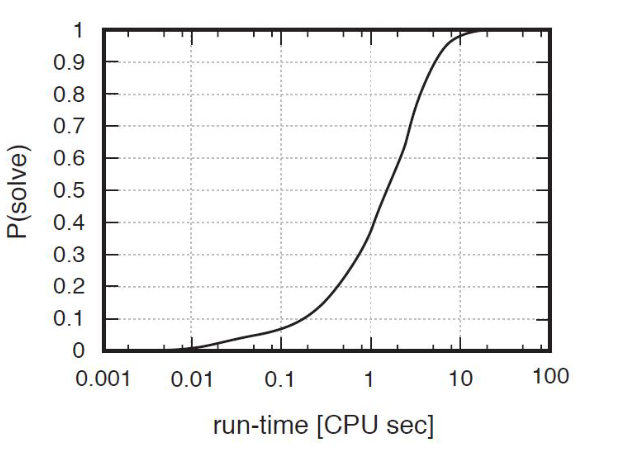
\includegraphics[width=0.75\columnwidth]{img/RTD1}
	\end{center}
	If given only $n$ as a parameter there are really slow and really fast instances, there could be another parameter which plays a role in the execution time. Essentially dividing $\overline{I}_n$ in further "sub-classes".\\
	
	If all influential parameters are identified and fixed, the RTD diagram degenerates into a step function (all instances require the same time; zero probability under a value, 1 over).\\
	
	\newpage
	
	The Run Time Distribution (RTD) diagram is
	\begin{itemize}
		\item \textbf{monotone nondecreasing:} more instances are solved in longer times
		\item \textbf{step-wise and right-continuous:} the graph steps up at each $T (i )$
		\item \textbf{equal to zero for $t < 0$:} no instance is solved in negative time
		\item \textbf{equal to} $1$ \textbf{for} $t \geq \max_{i \in \overline{I}} T(i)$: all are solved within the longest time
	\end{itemize}
	\begin{center}
		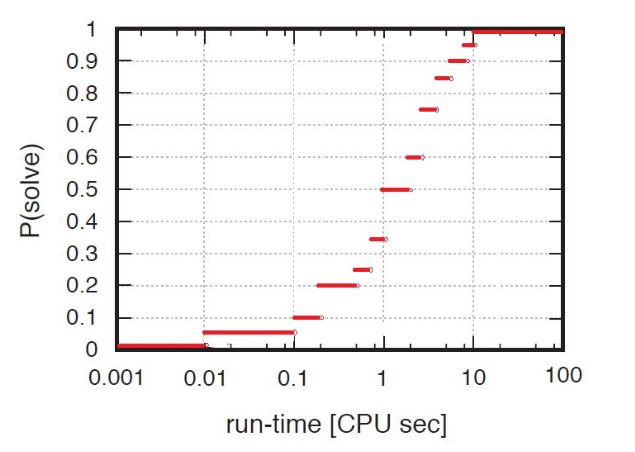
\includegraphics[width=0.75\columnwidth]{img/RTD2}
	\end{center}
	For large benchmark samples, the plot looks continuous, but it is not.\\
	
	The graph goes up by steps because it shows how many instances (in percent) are solved given a certain amount of time. \\
	If there is a big enough number of instances the number of "steps" will increase, giving the impression of a continuous graph.\\
	
	In order to \textbf{build the diagram}:
	\begin{enumerate}
		\item \textbf{run} the algorithm \textbf{on each instance} $i \in \overline{I}$
		\item \textbf{build the set} $T_A (\overline{I}) = \left\{T_A (i): \, i \in \overline{I}\right\}$ (it's just a set of numbers)
		\item \textbf{sort} $T_A (\overline{I})$ by \textbf{non-decreasing} values: $t_1 \leq \, ... \, \leq  t_{|\overline{I}|}$
		\item \textbf{plot the points} $\left(t_j, \frac{j}{|\overline{I}|}\right)$ for $j = 1, \, ... \, , |\overline{I}|$ (for each $t_j$ , only the highest) and the horizontal segments (close on the left, open on the right)
	\end{enumerate}
	
	\newpage
	
	\paragraph{Scaling diagram:} this diagram describes the dependence of $T (i )$ on the size $n (i )$
	\begin{itemize}
		\item \textbf{generate a sequence of values} of $n$ and a sample $\overline{I}_n$ for each value (generate a benchmark sample for each size)
		\item \textbf{apply the algorithm} to each $I \in \overline{I}_n$ for all $n$ (all instances of each sub-benchmark for all the sizes)
		\item \textbf{sketch} all points $(n (i ) , T (i ))$ or the mean points $\left(n, \frac{\sum_{i \in \overline{I}_n} T(i)}{|\overline{I}_n|}\right)$ 
		\item assume an \textbf{interpolating function}
		\item \textbf{estimate the numerical parameters} of the interpolating function
	\end{itemize}
	It shows how the computational time scales in relation to the size of the instance.
	\begin{center}
		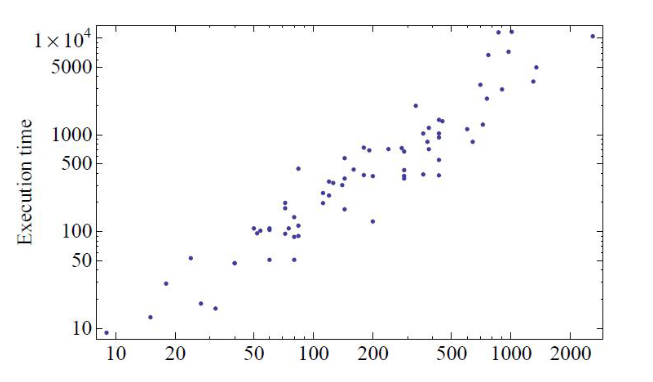
\includegraphics[width=0.7\columnwidth]{img/SD1}
	\end{center}
	This analysis provides an \textbf{empirical average-case complexity}
	\begin{itemize}
		\item with \textbf{well-determined multiplying factors} (instead of $c_1$ and $c_2$)
		\item \textbf{not larger} than the \textbf{worst-case one} (it also includes easy instances)
	\end{itemize}
	
	\newpage
	
	The correct family of interpolating functions can be suggested
	\begin{itemize}
		\item by a \textbf{theoretical analysis} (studying the algorithm)
		\item by \textbf{graphical manipulations}
	\end{itemize}
	(Linear interpolation is usually the right tool).\\
	
	The \textbf{scaling diagram turns into a straight line} when
	\begin{itemize}
		\item an \textbf{exponential algorithm} is represented on a \textbf{semi-logarithmic scale} (the logarithm is applied only to the time axis)
		$$ \log_2 T(n) = \alpha n + \beta \Leftrightarrow T(n) = 2^\beta \left(2^\alpha\right)^n $$
		if the $\log$ of the time is a linear function of the size, necessarily the algorithm is exponential.\\
		I see the time goes up a lot, I have reason to suspect the algorithm is exponential from the theoretical analysis $\implies$ I try to use a logarithmic scale for the time.\\
		
		\item a \textbf{polynomial algorithm} is represented on a \textbf{logarithmic scale} (the logarithm is applied to both axes)
		$$ \log_2 T(n) = \alpha\log_2 n + \beta \Leftrightarrow T(n) = 2^\beta n^\alpha $$
		the $\log$ of the time is a $\log$ function of the size, then the computational time is polynomial ($\alpha$ is the exponent).\\
	\end{itemize}
	
	\newpage
	
	\subsubsection{Analysis of the quality of the solution}
	The \textbf{Solution Quality Distribution (SQD) diagram} is the plot of the \textbf{distribution function} of $\delta_A (i)$ \textbf{on} $\overline{I}$ (relative difference on the benchmark)
	$$ F_{\delta_A} (\alpha) = Pr \left[\delta_A (i) \leq \alpha\right] \text{ for each } \alpha \in \mathbb{R} $$
	\begin{center}
		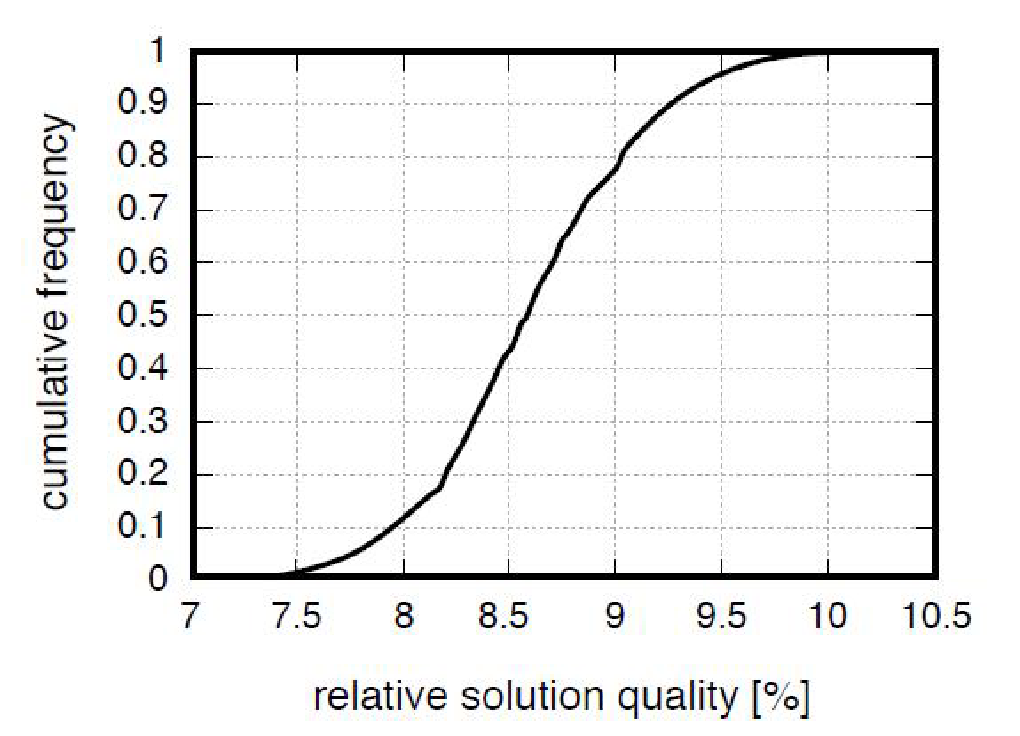
\includegraphics[width=0.7\columnwidth]{img/SQD1}
	\end{center}
	It plots the probability that the relative difference is smaller than a value $\alpha$, for each possible value of $\alpha$. \\
	
	One axis is the frequency, the other is the relative difference, it basically answers the question "how many instances got this $\delta_A$ or less?". \\
	
	\newpage
	
	For any algorithm, the \textbf{distribution function} of $\delta_A (i)$ is
	\begin{itemize}
		\item \textbf{monotone non-decreasing:} more instances are solved with worse gaps
		\item \textbf{step-wise and right-continuous:} the graph steps up at each $\delta (i)$
		\item \textbf{equal to zero for $\alpha < 0$:} no instance is solved with negative gap
		\item \textbf{equal to $1$ for $\alpha \geq \max_{i \in \overline{I}} \delta (i)$:} all are solved within the largest gap
	\end{itemize}
	\begin{center}
		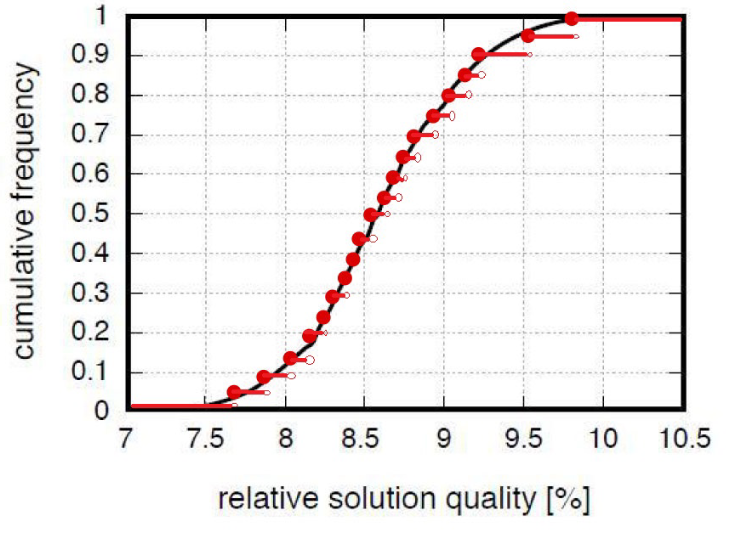
\includegraphics[width=0.7\columnwidth]{img/SQD2}
	\end{center}
	As with the RTD, the more instances you have the more this diagram looks continuous.\\
	
	If $A$ is an
	\begin{itemize}
		\item exact algorithm, it is a step-wise function, equal to $1$ for all $\alpha \geq 0$
		\item $\overline{\alpha}$-approximated algorithm, it is a function equal to $1$ for large $\alpha$
	\end{itemize}
	\nn
	
	In order to \textbf{build the diagram}:
	\begin{enumerate}
		\item \textbf{run the algorithm on each instance} $i \in \overline{I}$
		\item \textbf{build the set} $\Delta_A (\overline{I}) = \left\{\delta_A (i): \, i \in \overline{I} \right\}$, the relative difference for each instance (you need the optimum, could be approximated)
		\item \textbf{sort} $\Delta_A (\overline{I})$ non-decreasing values: $\delta_1 \leq \, ... \, \leq \delta_{|\overline{I}|}$
		\item \textbf{plot points} $\left(\delta_j, \frac{j}{|\overline{I}|}\right)$ for $j = 1, \, ... \, , |\overline{I}|$ (for each $\delta_j$, only the highest) and the horizontal segments (close on the left, open on the right)
	\end{enumerate}

	\newpage
	
	\paragraph{Parametric SQD diagrams:} Given the theoretical and practical problems to build a \textbf{meaningful sample} often the \textbf{diagram is parameterized} with respect to
	\begin{itemize}
		\item a \textbf{descriptive parameter of the instances} (size, density, ...)
		\item a \textbf{parameter} of the \textbf{probability distribution assumed} for the \textbf{instances} (expected value or variance of the costs, ...)
	\end{itemize}
	\begin{center}
		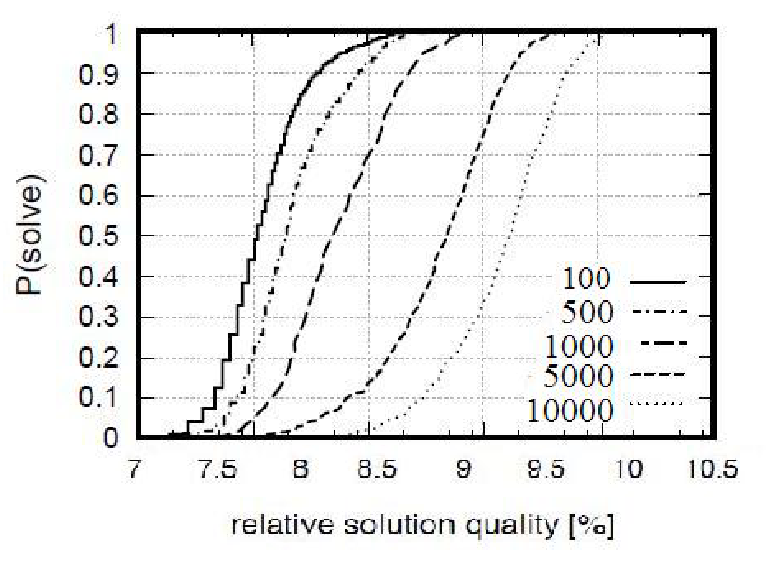
\includegraphics[width=0.7\columnwidth]{img/SQD3}
	\end{center}
	The conclusions are more limited, but the \textbf{sample is more significant}. General trends can be highlighted (what happens as size increases?).\\
	
	It's basically dividing the benchmark set into sub-benchmarks, following some parameters (such as size, ecc...), to get the solution quality in relation to those parameters. \\
	
	\newpage
	
	\paragraph{Comparison between algorithms with the SQDs:} How to determine whether an \textbf{algorithm is better than another}? (for simplicity's sake, the algorithms take the same time)
	\begin{itemize}
		\item \textbf{strict dominance:} it obtains better results on all instances
		$$ \delta_{A_2} (i) \leq \delta_{A_1} (i) \text{ for each } i \in I $$
		This usually happens only in trivial cases (e.g., $A_2$ "includes" $A_1$). $A_2$ is always better. \\
		
		\item \textbf{probabilistic dominance:} the distribution function has higher values for every value of $\alpha$
		$$ F_{\delta_{A_2}} (\alpha) \geq F_{\delta_{A_1}} (\alpha) \text{ for all } \alpha \in \mathbb{R} $$
		the SQD of $A_2$ is larger or equal than the one for $A_1$ (is "above", if you set a certain threshold of "quality" $A_2$ has a better occurrence rate).\\
	\end{itemize}
	
	The following plot shows no dominance, but $A_1$ is less "robust" than $A_2$: $A_1$ has results more dispersed than $A_2$ (both better and worse)
	\begin{center}
		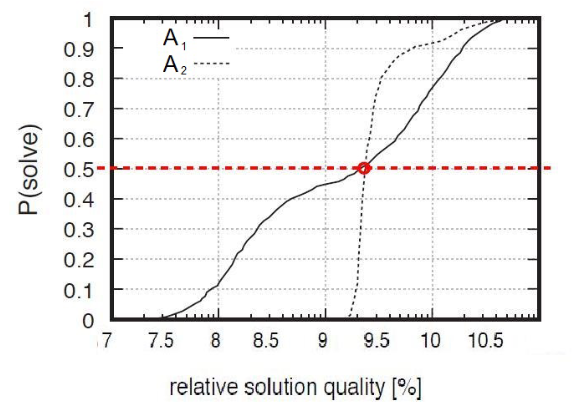
\includegraphics[width=0.7\columnwidth]{img/SQD4}
	\end{center}
	
	% End of L5
	
	\newpage
	
	\subsubsection{Compact statistical descriptions}
	The distribution function $F_{\delta_A}$ can be replaced or accompanied by more compact characterizations of the effectiveness of an algorithm.\\
	
	This typically involves classical \textbf{statistical indices} of 
	\begin{itemize}
		\item \textbf{position}, such as the sample mean
		$$ \overline{\delta}_A = \frac{\sum_{i \in \overline{I}} \delta_A (i)}{|\overline{I}|} $$
		\item \textbf{dispersion}, such as the sample variance
		$$ \overline{\sigma}_A^2 = \frac{\sum_{i \in \overline{I}} \left(\delta_A (i) - \overline{\delta}_A \right)^2}{|\overline{I}|} $$
	\end{itemize}
	These indices "\textbf{suffer}" from the influence of \textbf{outliers}.\\
	
	Other statistical indices are "stabler" and more detailed
	\begin{itemize}
		\item the \textbf{sample median}
		\item suitable \textbf{sample quantiles}
	\end{itemize}
	
	\newpage
	
	\subsubsection{Boxplots diagrams}
	\paragraph{Boxplot:} A graphic representation is the boxplot (or box and whiskers diagram)
	\begin{itemize}
		\item sample \textbf{median} ($q_{0.5}$)
		\item \textbf{lower} and \textbf{upper} sample \textbf{quartiles} ($q_{0.25}$ and $q_{0.75}$)
		\item the \textbf{extreme} sample values (often excluding the "outliers")
	\end{itemize}
	\begin{center}
		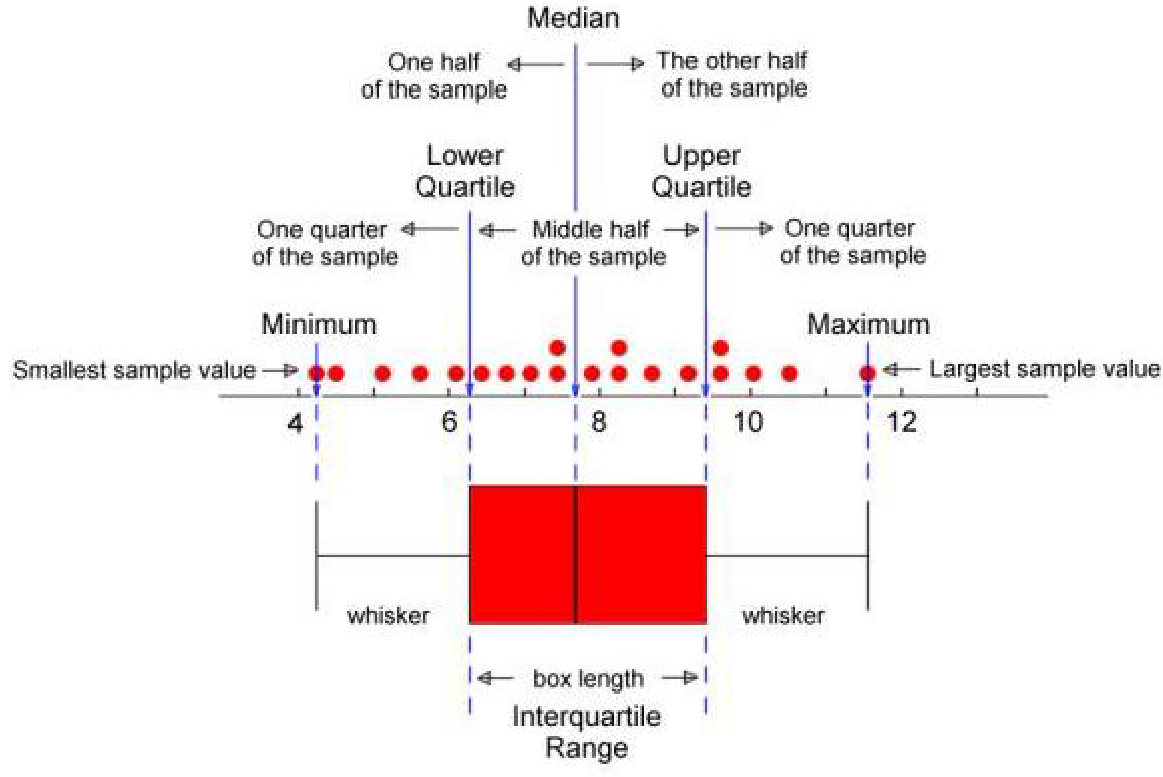
\includegraphics[width=0.9\columnwidth]{img/boxplot1}
	\end{center}
	On the $x$ axis there's the relative difference (in the example, from $4$ to $12$). The median is in the middle, the box represents the two middle quartiles, the whiskers represent the last two quartiles.\\
	
	To have a boxplot diagram you need to have: extreme values (upper and lower), lower and upper quartiles, median. If you have these values you can draw the diagram.\\
	
	\newpage
	
	\paragraph{Comparison between algorithms with boxplot diagrams:} A more compact comparison can be performed with boxplot diagrams (the dots represent outliers)
	\begin{center}
		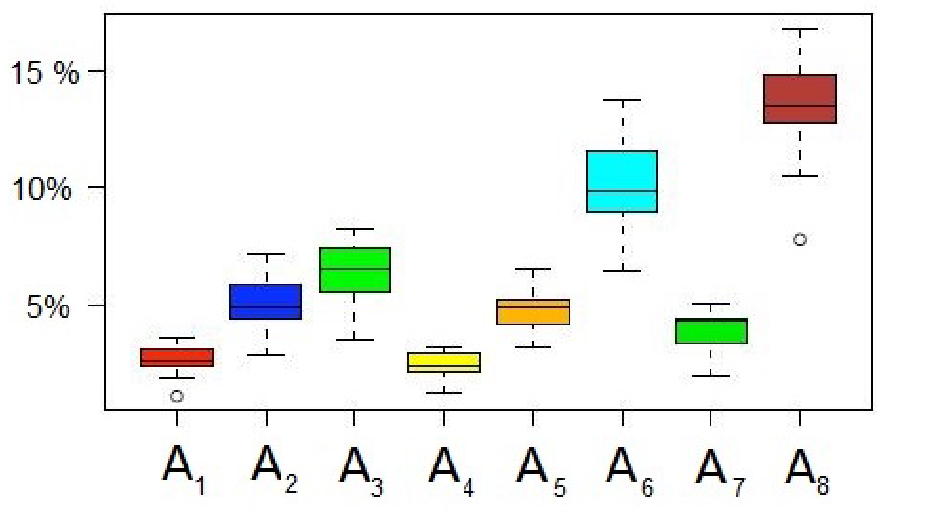
\includegraphics[width=0.9\columnwidth]{img/boxplot2}
	\end{center}
	\textbf{Necessary} conditions:
	\begin{center}
		\textbf{Strict dominance} $\implies$ \textbf{Probabilistic dominance} $\implies q_i \leq q_i ' (i = 1, \, ... \, , 5)$
	\end{center}
	Strict dominance holds only if probabilistic dominance holds. \\
	
	\textbf{Strict dominance} holds if a boxplot is \textbf{fully below the other} (e.g. $A_7 - A_8$).\\
	
	\textbf{Probabilistic dominance} holds only if \textbf{each} of the five \textbf{quartiles} is \textbf{not above} the corresponding \textbf{one of the other} algorithm (e.g. $A_2 - A_3$).\\
	
	Strict dominance means a box is fully below another, probabilistic dominance means a box is at least partially below another. Obviously the first implies the latter.\\
	
	\newpage
	
	\subsubsection{Relation between quality and computational time}
	Many heuristic algorithms find \textbf{several solutions} during their execution, instead of a single one, and consequently can be \textbf{terminated prematurely}.\\
	
	In particular, \textbf{metaheuristics} (random steps or memory mechanisms) have a computational time $t$ fixed by the user and potentially unlimited; they often find a solution and improve on it.\\
	
	Let $\delta_A (i, t)$ be the \textbf{relative difference} reached by $A$ at time $t$ on instance $i$.\\
	As a function of time $t$, $\delta_A (i, t)$ is
	\begin{itemize}
		\item $+ \infty$ if $A$ has \textbf{not} yet \textbf{found} a feasible \textbf{solution} at time $t$
		\item step-wise \textbf{monotone nonincreasing} (the solution doesn't get worse)
		\item \textbf{constant} after the regular \textbf{termination} ($t \geq T (i)$; after the termination of the algorithm the solution doesn't improve)
	\end{itemize}
	
	\vfill
	
	\paragraph{Randomized algorithms:} For randomized algorithms the relative difference $\delta_A (i, \omega, t)$ depends on
	\begin{enumerate}
		\item the \textbf{instance} $i \in I$
		\item the \textbf{outcome} $\omega \in \Omega$ of the random experiment guiding the algorithm (the random seed)
		\item the \textbf{execution time} $t$
	\end{enumerate}
	
	Given a \textbf{fixed time}, these algorithms can be \textbf{tested}
	\begin{enumerate}
		\item on a \textbf{sample of instances} $\overline{I}$ with a \textbf{fixed seed} $\omega$
		\item on a \textbf{fixed instance} $i$ with a \textbf{batch of seeds} $\overline{\Omega}$ (different runs)
		\item on \textbf{several instances} with \textbf{several seeds} on each instance
	\end{enumerate}
	
	The results of \textbf{multiple runs} ($\overline{\Omega}$) are usually \textbf{summarized} providing both:
	\begin{itemize}
		\item the \textbf{minimum relative difference} $\delta_A^\ast (i, t)$ and the \textbf{total time} $|\overline{\Omega}|t$
		\item the \textbf{average relative difference} $\overline{\delta}_A (i, t)$ and the \textbf{single-run time} $t$
	\end{itemize}
	
	\newpage
	
	\subsection{Classification}
	The relation between solution quality and computational time allows to \textbf{classify the algorithms} into:
	\begin{itemize}
		\item \textbf{complete:} for each instance $i \in I$, find the optimum in finite time
		$$ \exists \overline{t}_i \in \mathbb{R}^+ : \, \delta_A (i, t) = 0 \text{ for each } t \geq \overline{t}, \, i \in I $$
		(Another name for exact algorithms) for every instance the algorithm gives the optimum in finite time. \\
		
		\item \textbf{probabilistically approximately complete:} for each instance $i \in I$, find the optimum with probability converging to $1$ as $t \rightarrow + \infty$
		$$ \lim_{t \rightarrow + \infty} Pr \left[\delta_A (i, t) = 0\right] = 1 \text{ for each } i \in I $$
		(Many randomized metaheuristics) for all instances, the probability of getting an exact solution converges to 1, given enough time. \\
		
		\item \textbf{essentially incomplete:} for some instances $i \in I$, find the optimum with probability strictly $< 1$ as $t \rightarrow + \infty$
		$$ \exists i \in I: \, \lim_{t \rightarrow + \infty} Pr \left[\delta_A (i, t) = 0 \right] < 1 $$
		(Most greedy algorithms, local search algorithms, ...) even given infinite time, some instances can't get to the exact solution. \\
	\end{itemize}
	
	\newpage
	
	\subsubsection{Beyond the optimum, a generalization}
	An obvious generalization \textbf{replaces} the search for the \textbf{optimum} with that for a \textbf{given level of approximation}
	δA (I , t) = 0 → δA (I , t) ≤ α
	$$ \delta_A (i, t) = 0 \rightarrow \delta_A (i, t) \leq \alpha $$
	We're not searching for an exact solution, we're looking for a "good enough" solution, where the "good enough" is determined by $\alpha$.\\
	
	The algorithms can now be \textbf{classified} in
	\begin{itemize}
		\item \textbf{$\alpha$-complete algorithms:} for each instance $i \in I$, find an $\alpha$-approximated solution in finite time ($\alpha$-approximated algorithms).\\
		
		\item \textbf{probabilistically approximately $\alpha$-complete algorithms:} for each instance $i \in I$, find an $\alpha$-approximated solution with probability converging to $1$ as $t \rightarrow + \infty$.\\
		
		\item \textbf{essentially $\alpha$-incomplete algorithms:} for some instances $i \in I$, find an $\alpha$-approximated solution with probability strictly $< 1$ as $t \rightarrow +\infty$
	\end{itemize}
	
	In conclusion, every algorithm provides a \textbf{compromise} between
	\begin{itemize}
		\item a \textbf{quality measure}, described by the threshold $\alpha$
		\item a \textbf{time measure}, described by the threshold $t$
	\end{itemize}
	
	\newpage
	
	\subsubsection{Probability of success}
	Let the \textbf{success probability} $\pi_{A, n} (\alpha, t)$ be the probability that algorithm $A$ finds in \textbf{time} $\leq t$ a solution with a \textbf{gap} $\leq \alpha$ on an instance of \textbf{size} $n$
	$$ \pi_{A, n} (\alpha, t) = Pr \left[\delta_A (i, t) \leq \alpha | i \in I_n, \, \omega \in \Omega \right]$$
	\begin{center}
		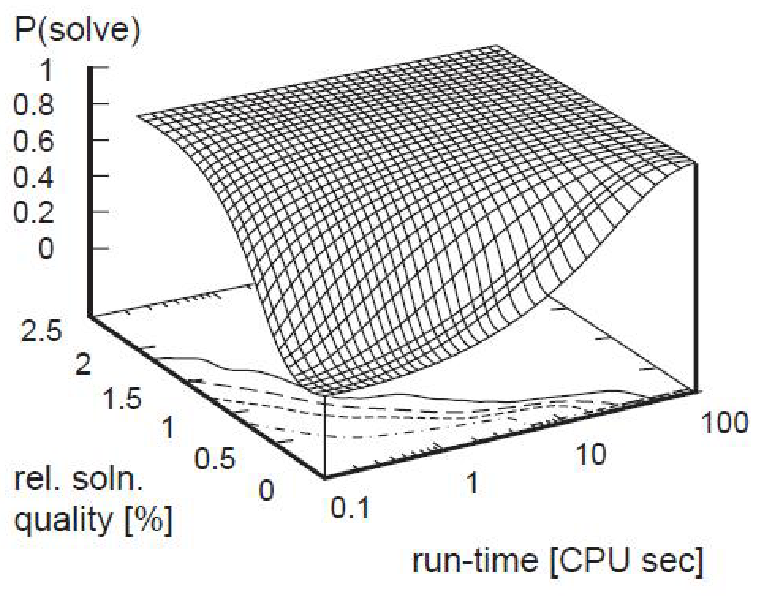
\includegraphics[width=0.7\columnwidth]{img/Psucc1}
	\end{center}
	This yields different secondary diagrams, derived from the time, solution quality and probability of solving.\\
	
	\newpage
	
	\paragraph{Qualified Run Time Distribution (QRTD) diagrams:} The QRTD diagrams describe the profile of the \textbf{time required} to \textbf{reach} a specified \textbf{level of quality}.
	\begin{center}
		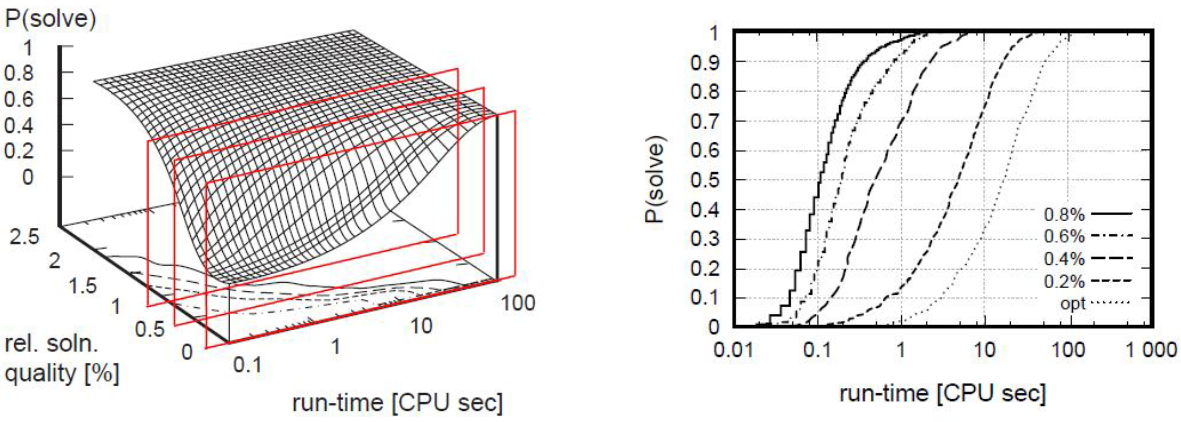
\includegraphics[width=\columnwidth]{img/QRTD1}
	\end{center}
	
	This is fixing the quality of the solution $\alpha$ and showing how the probability of getting such quality changes in relation to computational time.\\
	
	They are useful when the computational time is not a tight resource.\\
	
	If the algorithm is
	\begin{itemize}
		\item complete, all diagrams reach $1$ in finite time
		\item $\overline{\alpha}$-complete, all diagrams with $\alpha \geq \overline{\alpha}$ reach $1$ in finite time
		\item $\overline{\alpha}$-incomplete, all diagrams with $\alpha \leq \overline{\alpha}$ do not reach $1$
	\end{itemize}
	
	\newpage
	
	\paragraph{Timed Solution Quality Distribution (TSQD) diagrams:} The TSQD diagrams describe the profile of the \textbf{level of quality} reached in a \textbf{given computational time}
	\begin{center}
		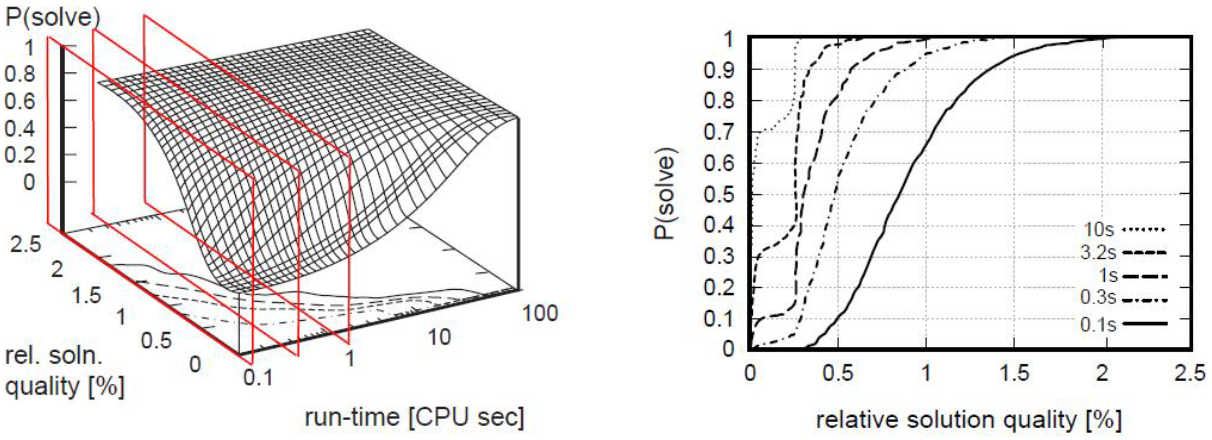
\includegraphics[width=\columnwidth]{img/TSQD1}
	\end{center}
	
	This is fixing the computational time and showing what's the probability of getting a certain quality of solution in that given time.\\
	
	They are useful when the computational time is a tight resource.\\
	
	If the algorithm is
	\begin{itemize}
		\item complete, all diagrams with a sufficient $t$ are step functions in $\alpha = 0$
		\item $\overline{\alpha}$-complete, all diagrams with a sufficient $t$ reach $1$ in $\alpha = \overline{\alpha}$
		\item probab. approx. $\overline{\alpha}$-complete, the diagrams converge to $1$ in $\alpha = \overline{\alpha}$
		\item $\overline{\alpha}$-incomplete, all diagrams keep $< 1$ in $\alpha = \overline{\alpha}$
	\end{itemize}
	
	\newpage
	
	\paragraph{Solution Quality statistics over Time (SQT) diagrams:} One can also draw the \textbf{level lines} associated to \textbf{different quantiles}. 
	\begin{center}
		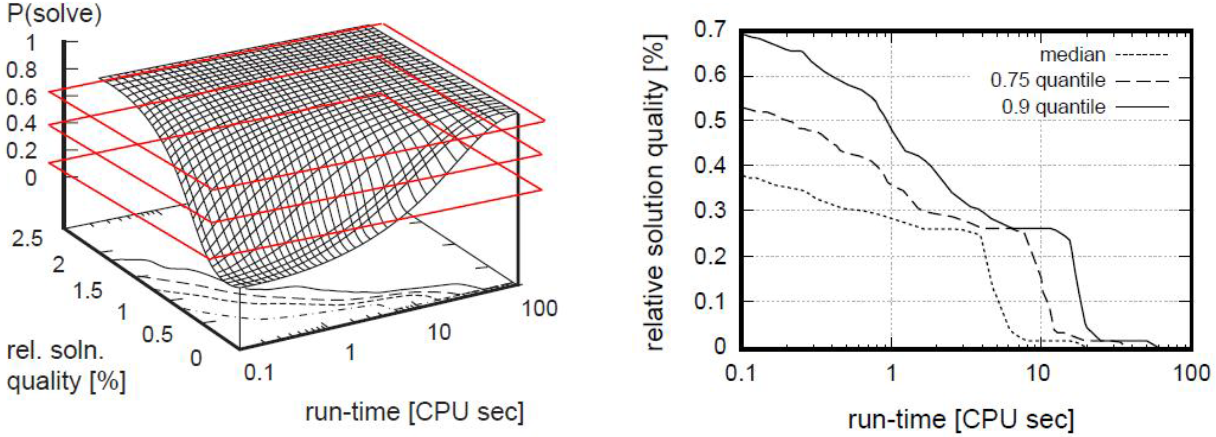
\includegraphics[width=\columnwidth]{img/SQT1}
	\end{center}
	
	This shows how the solution quality changes in relation to the computational time, given a fixed probability of getting such quality of solution. \\
	
	They describe the compromise between quality and computational time.\\
	
	For a robust algorithm the level lines are very close to each other.\\
	
	\newpage
	
	\subsection{Statistical tests (Wilcoxon's test)}
	Diagrams and boxplots are qualitative: how do you \textbf{evaluate} quantitatively if the \textbf{empirical difference between algorithms} $A_1$ and $A_2$ is \textbf{significant}?\\
	
	\textbf{Wilcoxon's test} focuses on effectiveness (neglecting robustness)
	\begin{itemize}
		\item $f_{A_1} (i) - f_{A_2} (i)$ is a \textbf{random variable defined on the sample space} $I$, objective function, measures the quality; if it's negative $A_1$ is better than $A_2$ and vice versa (assuming a minimization problem).\\
		
		\item Formulate a \textbf{null hypothesis} $H_0$ according to which the \textbf{theoretical median} of $f_{A_1} (i) - f_{A_2} (i)$ is \textbf{zero} (they are equivalent, half the time one is better, switching for the other half).\\
		
		\item Extract a \textbf{sample of instances} $\overline{I}$ and \textbf{run} the \textbf{two algorithms} on it, obtaining a \textbf{sample of pairs of values} $(f_{A_1}, f_{A_2})$.\\
		
		\item Compute the \textbf{probability} $p$ of \textbf{obtaining the observed result} (that particular set of pairs) or a more "extreme" one (that set or less probable), assuming that $H_0$ is true (assuming it follows our hypothesis); is it just bad luck or is the hypothesis wrong? \\
		
		\item Set a \textbf{significance level} $\overline{p}$, that is the
		\begin{itemize}
			\item \textbf{maximum acceptable probability to reject} $H_0$ assuming that it is true
			\item that is, to consider \textbf{two identical medians as different}
			\item that is, to consider \textbf{two equivalent algorithms as differently effective} (referring to the median of the gap)
		\end{itemize}
		$\overline{p}$ is the probability above which we can say that the hypothesis follows our observed results.\\
		
		\item \textbf{reject} $H_0$ \textbf{when} $p < \overline{p}$
	\end{itemize}
	Typical values for the significance level are $\overline{p} = 5\%$ or $\overline{p} = 1\%$.\\
	
	\newpage
	
	\subsubsection{Assumptions} 
	It is a \textbf{nonparametric} test, that is, it does \textbf{not} make \textbf{assumptions} on the \textbf{probability distribution} of the tested \textbf{values}.\\
	
	It is useful to evaluate the performance of heuristic algorithms, because the \textbf{distribution of the result} $f_A (i )$ is \textbf{unknown}. \\
	
	It is based on the following \textbf{assumptions}:
	\begin{itemize}
		\item \textbf{all data} are \textbf{measured} at least on an \textbf{ordinal scale} (the specific values do not matter, only their relative size, you just need a sequence of levels, we use numbers so it's obviously verified)
		\item the two \textbf{data sets} are \textbf{matched} and \textbf{derive from the same population} (we apply $A_1$ and $A_2$ to the same instances, extracted from $I$, so it's always verified)
		\item each \textbf{pair of values is extracted independently} from the others (the instances are generated independently from one another, not always satisfied)
	\end{itemize}
	
	\newpage
	
	\subsubsection{Application}
	Application of the Wilcoxon's test: 
	\begin{enumerate}
		\item Compute the \textbf{absolute differences} $| f_{A_1} (i_j) − f_{A_2} (i_j)|$ for all $i_j \in \overline{I}$ (instance by instance).\\
		
		\item \textbf{Sort} them by \textbf{increasing} values and assign a \textbf{rank} $R_j$ to each one; all zero-differences can be removed; in case of ties, all should have an average.\\
		We're getting the sum of all the ranks, which is proportional to the difference, this serves the purpose of considering if the difference itself is large or small and not only the number of instances an algorithm has "won".\\
		
		\item Separately \textbf{sum the ranks of the pairs} with a positive difference and those of the pairs with a negative difference
		$$ 
		\begin{cases}
			W^+ & = \sum_{j:f_{A_1} (i_j) > f_{A_2} (i_j)} R_j \\
			W^- & = \sum_{j:f_{A_1} (i_j) < f_{A_2} (i_j)} R_j
		\end{cases}
		$$
		If the null hypothesis $H_0$ were true, the two sums should be equal.\\
		Each positive is summed together, same with the negatives, if the algorithms are truly equivalent (as per the null hypothesis), these should be the same, i.e. $W^+ - W^-$ should be $0$. We're computing the sum of the ranks for the instances where the first algorithm is better than the second and vice versa.\\
		
		\item The \textbf{difference} $W^+ - W^-$ allows to \textbf{compute} the \textbf{value of} $p$: each of the $|\overline{I}|$ differences can be positive or negative: $2^{|\overline{I}|}$ outcomes; $p$ is the fraction with $|W^+ - W^-|$ equal or larger than the observed value.\\
		
		\item if $p < \overline{p}$, the \textbf{difference is significant} and
		\begin{itemize}
			\item if $W^+ < W^-$, $A_1$ is better than $A_2$
			\item if $W^+ > W^-$, $A_1$ is worse than $A_2$
		\end{itemize}
	\end{enumerate}
	
	\newpage
	
	\paragraph{Computation of the $p$-value:} The value of $p$ (distribution of probability) is usually
	\begin{itemize}
		\item \textbf{computed explicitly} by enumeration when $|\overline{I}| < 20$; which possible cases give us each value?
		\item \textbf{approximated} with a \textbf{normal distribution} when $|\overline{I}| \geq 20$; there's a lot of cases, it can be approximated
	\end{itemize}
	\begin{center}
		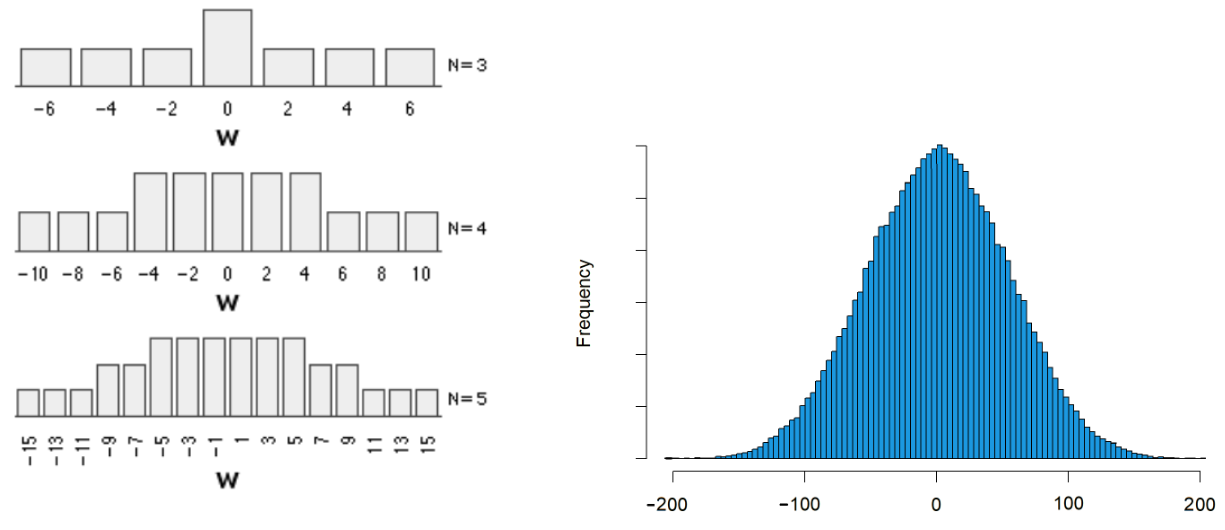
\includegraphics[width=\columnwidth]{img/pval1}
	\end{center}
	Of course, pre-computed tables also exist.\\
	
	We get the probability distribution and we observe the probability of the value we got, then we need to evaluate if it's reasonable or if it's a significant result. \\
	
	\newpage
	
	\paragraph{Possible conclusions:} Wilcoxon's test can suggest
	\begin{itemize}
		\item that \textbf{one of the two algorithms is significantly better} than the other
		\item that the \textbf{two algorithms are statistically equivalent} (but take it as a stochastic response, and keep an eye on $p$)
	\end{itemize}
	
	If the sample includes instances of different kinds, two algorithms could be \textbf{overall equivalent}, but \textbf{nonequivalent} on the \textbf{single classes} of instances.\\
	
	\textbf{Dividing the sample} could reveal
	\begin{itemize}
		\item classes of instances for which $A_1$ is better
		\item classes of instances for which $A_2$ is better
		\item classes of instances for which the two algorithms are equivalent
	\end{itemize}
	but multiplying questions means getting some wrong answers by chance (FWER = Family-Wise Error Rate). \\
	
	What about testing $\delta_A (i)$ instead of $f_A (i )$? (Open question).\\
	
	% End of L6
	
	\newpage
	
	\section{Constructive Heuristics}
	In Combinatorial Optimization every solution $x$ is a subset of the ground set $B$.\\
	
	Essentially we want to add an element at a time to an empty subset until it doesn't make sense anymore to have new elements.\\
	
	A constructive heuristic \textbf{updates a subset} $x^{(t)}$ step by step
	\begin{enumerate}
		\item \textbf{start} from an \textbf{empty subset}: $x^{(0)} = \emptyset$ (obviously a subset of any optimal solution)
		\item \textbf{stop} when a \textbf{termination condition} holds (the following subsets cannot be optimal solutions, there are no more elements to be added that lead to an optimal solution)
		\item \textbf{select} the "\textbf{best}" element $i^{(t)} \in B \setminus x$ among the "acceptable" ones (parameter which needs to be determined) at the current step $t$ (try and keep $x^{(t)}$ within a feasible and optimal solution)
		\item \textbf{add} $i^{(t)}$ to the \textbf{current subset} $x^{(t)}: \, x^{(t+1)} := x^{(t)} \cup \{i^{(t)}\}$ (the selection can never be undone!)
		\item go \textbf{back to point 2}
	\end{enumerate}
	Such processes admit a nice modeling tool.\\
	
	\newpage
	
	\subsection{Construction Graph}
	Every construction heuristic $A$ defines a \textbf{construction graph}
	\begin{itemize}
		\item the \textbf{node set} $F_A \subseteq 2^B$ (\textbf{search space}) is the collection of all subsets $x \subseteq B$ acceptable for $A$
		\item the \textbf{arc set} is the collection of all pairs $(x, x \cup \{i\})$ such that $x \in F_A$, $i \in B \setminus x$ and $x \cup \{i\} \in F_A$ (connects $x$ with $x$ plus one element). The arcs represent the elementary extensions of the acceptable subsets
	\end{itemize}
	
	It's a directed graph in which the nodes compose the search space, dependent on $A$, and the arcs link all the element of the search space to every element with a cardinality of one more. Essentially the nodes are all the possible subsets, while the arcs represent all the possible connections (additions of elements) for each node (subset).\\
	
	The construction graph is by definition \textbf{acyclic}.\\
	
	Each possible execution of $A$ is a \textbf{maximal path of the construction graph}
	\begin{itemize}
		\item \textbf{from} the empty subset $x = \emptyset$
		\item to a subset $x$ that \textbf{cannot be acceptably extended} (and hopefully a feasible solution)
	\end{itemize}
	$$ \Delta^+_A (x) = \left\{i \in B \setminus x : \, x \cup \left\{i\right\} \in F_A \right\} = \emptyset $$
	
	\newpage
	
	\paragraph{Example}
	\begin{center}
		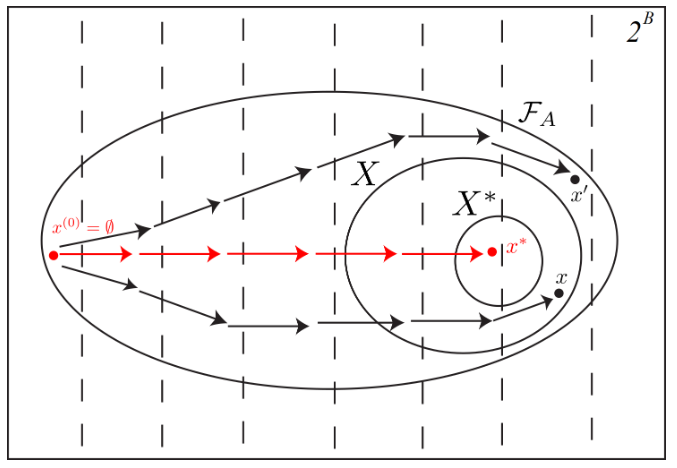
\includegraphics[width=0.8\columnwidth]{img/CGraph1}
	\end{center}
	The algorithm visits a \textbf{sequence of subsets} $\emptyset = x^{(0)} \subset \, ... \, \subset x^{(t_f)}$ terminating
	\begin{itemize}
		\item in an \textbf{optimal solution} $x^\ast \in X^\ast$ (Example: MST problem, both with $F_{Kruskal}$ and $F_{Prim}$)
		\item in a \textbf{nonoptimal feasible solution} $x \in X$ (Example: KP, MDP, etc...)
		\item in an \textbf{unfeasible subset} $x'$ (Example: TSP on a noncomplete graph)
	\end{itemize}
	
	\newpage
	
	\subsubsection{Termination condition} 
	A constructive heuristic $A$ \textbf{terminates} when
	\begin{itemize}
		\item the current \textbf{subset} $x^{(t)}$ has \textbf{no outgoing arc}
		$$ \Delta^+_A \left(x^{(t)}\right) = \left\{i \in B \setminus x^{(t)} : \, x^{(t)} \cup \left\{i\right\} \in F_A \right\} = \emptyset $$
		$\Delta^+_A \left(x^{(t)}\right)$ represents the subset of the ground set that can be added in $x^{(t)}$ in an acceptable manner for algorithm $A$ (what I can add to our solution).\\
		
		\item that is, \textbf{extending} $x^{(t)}$ implies to \textbf{leave the search space} $F_A$
		$$ x^{(t)} \cup \left\{i\right\} \notin F_A \text{ for each } i \in B \setminus x^{(t)}$$
	\end{itemize}
	
	There is no arc going out of the node in the construction graph.\\
	
	The algorithm returns the \textbf{best solution visited} during the execution (usually the last one).\\
	
	Different behaviors are possible
	\begin{itemize}
		\item sometimes \textbf{all} visited \textbf{subsets} are \textbf{feasible} (e.g., KP)
		\item often the \textbf{last subset} is the only \textbf{feasible} solution
		\item $x^{(t)}$ could even \textbf{move in and out} of $X$ (or $X^\ast$; but this is uncommon)
		\item the path \textbf{can visit or not} $X$ and $X^\ast$
	\end{itemize}
	
	\newpage
	
	\subsubsection{Definition of the construction graph}
	Ideally, the \textbf{search space} $F_A$ should \textbf{include}
	\begin{itemize}
		\item the \textbf{empty subset}: $\emptyset \in F_A$ ($A$ starts from $\emptyset$)
		\item all \textbf{feasible solutions}: $X \subseteq F_A$ (maybe excluding provably nonoptimal solutions)
		\item \textbf{only subsets accessible from} $\emptyset$ (inaccessible subsets are useless)
	\end{itemize}
	
	Using $F_A$ requires a \textbf{fast inclusion test} to answer the decision problem:
	\begin{itemize}[label*=]
		\item "is subset $x^{(t)}$ acceptable?" ($x^{(t)} \in F_A$?)
	\end{itemize}
	or at least a \textbf{fast update test}: if $x^{(t)} \in F_A$, is $x^{(t)} \cup \{i\} \in F_A$? \\
	
	$F_A = \left\{x' \subseteq B : \, \exists x \in X : \, x' \subseteq x\right\}$ (subsets of feasible solutions, i.e. \textbf{partial solutions}) is a natural candidate, but its \textbf{inclusion test}
	\begin{itemize}[label*=]
		\item "is subset $x^{(t)}$ a partial solution?" ($\exists x \in X : \, x^{(t)} \subseteq x$?)
	\end{itemize}
	\textbf{generalizes} the feasibility problem ($\exists x \in X : \, \emptyset \subseteq x$?)
	\begin{itemize}[label*=]
		\item "is there any feasible solution?" ($\exists x \in X$?)
	\end{itemize}
	and could be NP-complete. In that case, one needs to \textbf{relax the search space}; include other subsets which may lead to more sub-optimal solutions, while making the acceptability test easier.\\
	
	Including a partial solution is like asking "is there a solution that includes this subset?" and could be an NP-complete problem, not always polynomial.\\
	
	If the \textbf{objective function} can be extended from $X$ to $F_A$, it looks natural to use the objective function as the \textbf{selection criteria}
	$$ \phi_A (i,x) = f \left(x \cup \left\{i\right\} \right)$$
	
	\newpage
	
	\paragraph{Examples of search spaces:} The search space $F_A$ may include:
	\begin{itemize}
		\item \textbf{All feasible solutions}
		$$ F_A = X $$
		In the KP, all subsets of feasible weight.\\
		
		\item \textbf{All partial (and all feasible) solutions}
		$$ F_A = \bigcup_{x \in X} 2^x $$
		In the MDP, all subsets of at most $k$ points.\\
		In Kruskal's algorithm for the MSTP, all spanning forests.\\
		
		\item \textbf{Only some special promising partial solutions}
		$$ F_A \subset \bigcup_{x \in X} 2^x $$
		In Prim's algorithm for the MSTP, all trees spanning a given vertex.\\
		
		\item \textbf{Some special subsets not sufficient to guarantee feasibility}
		$$ F_A \supset \bigcup_{x \in X} 2^x $$
		In the TSP, all subsets of arcs not including branching and sub-tours.\\
	\end{itemize}
	
	\newpage
	
	\subsection{Effectiveness and Efficiency}
	A constructive algorithm $A$ finds the optimum when at \textbf{each step} $t$ the current subset $x^{(t)}$ \textbf{is included} in at least one \textbf{optimal solution}. An exact algorithm always keeps an open way to an optimal solution.\\
	This property holds in $x^{(0)} = \emptyset$, but is usually lost at some step $t$,\\
	
	A constructive algorithm performs at \textbf{most} $n = |B|$ \textbf{steps} (can't add more element than the whole ground set) consisting of 
	\begin{enumerate}
		\item the \textbf{construction} of $\Delta_A^+ (x)$
		\item the \textbf{evaluation} of $\phi_A (i,x)$ for each $i \in \Delta_A^+(x)$
		\item the \textbf{selection} of the element $i$ minimizing $\phi_A (i,x)$
		\item the \textbf{update} of $x$ (and auxiliary data structures)
	\end{enumerate}
	In general, the \textbf{complexity} is a \textbf{polynomial} of rather low order, dominated by the first two components
	$$ T_A (n) \in O\left(n \left(T_{\Delta_A^+} (n) + T_{\phi_A} (n)\right)\right) $$
	
	\newpage
	
	\subsection{General features}
	Constructive algorithms
	\begin{itemize}
		\item are \textbf{intuitive}
		\item are \textbf{simple} to design, analyze and implement
		\item are \textbf{very efficient} (usually low complexity)
		\item have a \textbf{strongly variable effectiveness}; they can range from providing an optimal solution on some problem to not even guaranteeing a feasible solution; on most problems they provide solutions of extremely variable quality, often low
	\end{itemize}
	It is fundamental to \textbf{study the problem} before the algorithm.\\
	
	\paragraph{When are they used?} Constructive algorithms are used
	\begin{itemize}
		\item when they \textbf{provide} the \textbf{optimal solution}
		\item when the \textbf{execution time} must be \textbf{very short} 
		\item when the \textbf{problem} has a \textbf{huge size} or requires heavy computation 
		\item as a \textbf{component for other algorithms}, for example as
		\begin{itemize}
			\item \textbf{starting phase} for exchange algorithms 
			\item \textbf{basic procedure} for recombination algorithms
		\end{itemize}
	\end{itemize}
	
	\paragraph{Remarkable case:} A particularly remarkable case is that in which
	\begin{itemize}
		\item the \textbf{objective function} is \textbf{extended} from $X$ to $F_A$
		\item the \textbf{selection criteria is the objective function}
		$$ \phi_A (i,x) = f\left(x \cup \left\{i\right\}\right) $$
	\end{itemize}
	This means that instead of minimizing the selection criteria (which is generic) I use the value of the objective function. It's a greedy algorithm, sometimes can be a good idea.\\
	
	\newpage
	
	\subsection{Examples}
	\subsubsection{The Fractional Knapsack Problem (FKP)}
	Select from a set of \textbf{objects of identical volume} a \textbf{maximum value subset} which could be contained in a \textbf{knapsack of limited capacity} (same as the KP but all the objects have the same volume).\\
	
	In the FKP the capacity simply imposes a \textbf{cardinality constraint}: the feasible solutions are those with $|x| \leq \lfloor V / v \rfloor$
	
	\begin{algorithm}
		\caption{Algorithm $GreedyFKP(i)$}
		\begin{algorithmic}
			\STATE $x := \emptyset$; $x^\ast := \emptyset$;
			\IF{$x \in X$} 
				\STATE $f^\ast := f(x)$ ;
			\ELSE
				\STATE $f^\ast := + \infty$;
			\ENDIF
			\WHILE{$|x| < \lfloor V/v \rfloor$}
				\STATE $i:= \arg \max_{i \in B \setminus x} \phi_i$;
				\STATE $x := x \cup \left\{i\right\}$;
				\IF{$x \in X$ and $f(x) > f^\ast$}
					\STATE $x^\ast := x$; $f^\ast := f(x)$;
				\ENDIF
			\ENDWHILE
			\RETURN ($x^\ast, f^\ast$)
		\end{algorithmic}
	\end{algorithm}
	
	\begin{itemize}
		\item Define $F_A = X$: subset $x$ can be extended as long as $|x| < \lfloor V/v \rfloor$
		\item Any or no element of $B \setminus x$ extends $x$ feasibly ($\Delta_A (x) = B \setminus x$ or $\emptyset$)
		\item The objective function is additive, and therefore
		$$ f(x \cup \left\{i\right\}) = f(x) + \phi_i \implies \arg \max_{i \in B \setminus x} f(x \cup \left\{i\right\}) = \arg \max_{i \in B \setminus x} \phi_i $$
		\item The last subset visited is the best solution found
	\end{itemize}
	Just add objects until the cardinality is reached, add the most valuable one each time. Each solution is better than the previous one, since it's larger.\\
	
	The algorithm always finds the optimal solution.\\
	
	\newpage
	
	\subsubsection{The Knapsack Problem} 
	Select from a set of objects of \textbf{different volume} a maximum value subset which could be contained in a knapsack of limited capacity.\\
	
	The algorithm is similar, the \textbf{differences} are:
	\begin{itemize}
		\item The set of elements that can be added is the subset of items which do not exceed the residual capacity
		
		\item The termination condition must check that there is at least one element that can extend the current solution
	\end{itemize}
	
	\begin{algorithm}
		\caption{Algorithm $GreedyKP(i)$}
		\begin{algorithmic}
			\STATE $x := \emptyset$; $x^\ast := \emptyset$; $f^\ast := 0$
			\WHILE{$\exists i \in B \setminus x : \, v_i \leq V - \sum_{j \in x} v_j$}
				\STATE $i := \arg \max_{i \in B \setminus x : \, v_i \leq V - \sum_{j \in x} v_j} \phi_i$
				\STATE $x := x \cup \left\{i\right\}$
			\ENDWHILE
			\RETURN ($x, f(x)$)
		\end{algorithmic}
	\end{algorithm}
	
	Define $F_A = X$: only some elements of $B \setminus x$ extend $x$ feasibly
	$$ \Delta_A^+ (x) = \left\{i \in B \setminus x: \, \sum_{j \in x} v_j + v_i \leq V \right\} $$
	
	The objective function is additive, and therefore
	$$ f\left(x \cup \left\{i\right\}\right) = f(x) + \phi_i \implies \arg \max_{i \in \Delta_A^+ (x)} f\left(x \cup \left\{i\right\}\right) = \arg \max_{i \in \Delta_A^+ (x)} \phi_i $$
	
	The last subset visited is the best solution found.\\
	
	\newpage
	
	\subsubsection{Traveling Salesman Problem}
	Given a directed graph and a cost function defined on the arcs, find a \textbf{minimum cost circuit visiting all the nodes} of the graph.\\
	
	Define $F_A$ as the collection of all subsets of arcs that form no sub-tour and keep a degree $\leq 1$ in all nodes, (it is a superset of the partial solutions). The constructive algorithm add each time the cheapest arc among those in $F_A$, until nothing can be added, that's the solution.\\
	
	The selection criteria is the objective function (it is additive, therefore equivalent to the cost of the new arc).
	
	\begin{algorithm}
		\caption{Algorithm $GreedyTSP(i)$}
		\begin{algorithmic}
			\STATE $x := \emptyset$; $x^\ast := \emptyset$;
			\STATE $f^\ast := + \infty$;
			\WHILE{$\Delta_A^+(x) \neq \emptyset$}
				\STATE $i := \arg \min_{i \in \Delta_A^+ (x)} c_i$;
				\STATE $x := x \cup \left\{i\right\}$;
			\ENDWHILE
			\IF{$x \in X$}
				\STATE $x^\ast := x$; $f^\ast := f(x)$;
			\ENDIF
			\RETURN ($x^\ast, f^\ast$)
		\end{algorithmic}
	\end{algorithm}
	Only the last subset visited can be feasible (if any!).\\
	
	\newpage
	
	\subsubsection{Maximum Diversity Problem}
	Select from a set of points a subset of $k$ points with the \textbf{maximum sum of the pairwise distances}.\\
	
	\begin{algorithm}
		\caption{Algorithm $GreedyMDP(i)$}
		\begin{algorithmic}
			\STATE $x := \emptyset$
			\WHILE{$|x| < k$}
				\STATE $i := \arg \max_{i \in B \setminus x} \sum_{j \in x} d_{ij}$
				\STATE $x := x \cup \left\{i\right\}$
			\ENDWHILE
			\RETURN ($x, f(x)$)
		\end{algorithmic}
	\end{algorithm}
	
	Define $F_A$ as the set of all partial solutions.\\
	
	The subset $x$ can be extended as long as $|x| < k$.\\
	
	Any element of $B \setminus x$ extends $x$ in a feasible way.\\
	
	The objective function is quadratic, and therefore
	$$ f(x \cup \left\{i\right\}) = f(x) + 2 \sum_{j \in x} d_{ij} + d_{ii} \implies \arg \max_{i \in B \setminus x} \sum_{j \in x} d_{ij} $$
	
	The last subset visited is the best (and only feasible) solution found.\\
	
	\newpage
	
	\subsubsection{Summary}
	A constructive heuristic $A$ \textbf{finds}
	\begin{itemize}
		\item The \textbf{optimum} when $\Delta_A^+ \left(x^{(t)}\right)$ and $\phi_A (i, x)$ guarantee that the current subset $x^{(t)}$ is \textbf{always included} in at least one \textbf{optimal solution}.\\
		
		\item A \textbf{feasible solution} when $\Delta_A^+ \left(x^{(t)}\right)$ guarantees that the current subset $x^{(t)}$ is \textbf{always included} in at least one \textbf{feasible solution}.\\
		
		\item A \textbf{general subset} when these \textbf{properties are lost} at some step $t$
	\end{itemize}
	
	An ideal constructive algorithm always keeps one open way to the optimal solution.\\
	
	In practice, some of these properties is usually lost at some step of the algorithm.\\
	
	%\newpage
	
	\subsubsection{Relevant Features}
	None of the above algorithms where able to find the optimum (except the FKP, examples not provided, but trust me).\\
	
	What features allow a constructive algorithm to \textbf{find the optimum}? 
	\begin{itemize}
		\item A \textbf{search space identical to the feasible region} ($F = X$)? (No, because this holds for both the fractional and general KP)
		\item A \textbf{cardinality-constrained problem}? (It would explain failing on the KP, but not on the MDP and TSP)
		\item An \textbf{additive objective function}? (It does not explain failing on the TSP)
	\end{itemize}
	
	There is \textbf{no general characterization} of the problems solved exactly by constructive algorithms.\\
	
	But there are characterizations for wide classes of problems.\\
	
	\newpage
	
	\subsection{The additive case}
	Assume that
	\begin{enumerate}
		\item the \textbf{objective function} is \textbf{additive}
		$$ \exists \phi: \, B \rightarrow \mathbb{N}: \, f(x) = \sum_{i \in x} \phi_i $$
		
		\item the \textbf{solutions} are the \textbf{bases} (maximal subsets) of the \textbf{search space}
		$$ X = B_F = \left\{Y \in F: \, \not \exists Y' \in F: \, Y \subset Y' \right\} $$
		The maximal subsets of the search space $F$, there are no other subsets $Y'$ such that $Y$ is fully included in $Y'$ (can't be bigger).
	\end{enumerate}
	
	It is a very frequent case (KP, MAX-SAT, TSP, but not MDP, SCP).\\
	
	In this case, the constructive algorithm always finds the optimal solution if and only if $(B, F)$ is a \textbf{matroid embedding}.\\
	
	Since the definition of matroid embedding is rather complex, let us focus on some important structures
	\begin{itemize}
		\item greedoids (necessary condition)
		\item matroids or greedoids with the strong exchange property (sufficient)
	\end{itemize}
	
	\newpage
	
	\subsubsection{Greedoids}
	A \textbf{greedoid} $(B, F)$ (ground set, search space) with $F \subseteq 2^B$ is a \textbf{pair} such that
	\begin{itemize}
		\item \textbf{Trivial axiom:} $\emptyset \in F$.\\
		The empty set is acceptable. \\
		A greedy algorithm starts from the empty set so it must be included.\\
		
		\item \textbf{Accessibility axiom:} if $x \in F$ and $x 6\neq \emptyset$ then $\exists i \in x : \, x \setminus \{i\} \in F$.\\
		Any acceptable subset can be built adding elements in suitable order. Putting element in a given order creates a path through the search space.\\
		If you have a not empty subset in the search space, it's always possible to find an element of the subset that can be removed leaving the result in the search space.\\
		
		\item \textbf{Exchange axiom:} if $x, y \in F$ with $|x| = |y| + 1$, then $\exists i \in x \setminus y$ such that $y \cup \{i\} \in F$.\\
		Any acceptable subset can be extended with a suitable element of any other acceptable subset of larger cardinality.\\
		Two subsets in the search space, one has one more element than the second (cardinality $+1$), you can always find at least one element which is only in the larger subset and can be added to the smaller one in a way that results in another valid subset ($\in F$).\\
	\end{itemize}
	
	The exchange axiom implies that \textbf{all bases have the same cardinality}. \\
	If you consider two bases and assume them of different cardinality the axiom says that you can always take an element from the larger and put it into the smaller, while remaining in the search space. This would negate the axiom.\\
	
	All of these conditions
	\begin{itemize}
		\item hold in the fractional KP, MST problem (both Kruskal and Prim), ...
		\item do not hold in the general KP, TSP, ...
		\item hold in the MDP, but the objective function is not additive
	\end{itemize}
	Greedoids \textbf{make greedy algorithms possible}, but not necessarily exact.\\
	
	\newpage
	
	\subsubsection{Matroids}
	A matroid is a \textbf{set system} $(B, F)$ with $F \subseteq 2^B$ such that
	\begin{itemize}
		\item \textbf{Trivial axiom:} $\emptyset \in F$.\\
		
		\item \textbf{Heredity axiom:} if $x \in F$ and $y \subset x$ then $y \in F$.\\
		Any acceptable subset can be built adding its elements in any order.\\
		For any subset inside the search space, its subsets are also inside the search space.\\
		
		\item \textbf{Exchange axiom:} if $x, y \in F$ with $|x| = |y| + 1$, then $\exists i \in x \setminus y$ such that $y \cup \{i\} \in F$.\\
		Any acceptable subset can be extended with a suitable element of any other subset of larger cardinality.\\
	\end{itemize}
	
	The heredity axiom is a \textbf{stronger version of accessibility}
	\begin{itemize}
		\item it holds in Kruskal's search space for the MST problem
		\item it does not hold in Prim’s search space for the MST problem
	\end{itemize}
	
	
	\paragraph{Uniform matroid: fractional and general knapsack}
	$$ F = \left\{x \subseteq B : \, |x| \leq \lfloor V / v \rfloor \right\}$$
	
	\begin{itemize}
		\item Trivial axiom: the empty set respects the cardinality constraint
		\item Heredity axiom: if $x$ respects the cardinality constraint, all of its subsets also respect it
		\item Exchange axiom: if $x$ and $y$ respect the cardinality constraint and $|x| = |y| + 1$, one can always add a suitable element of $x$ to $y$ without violating the cardinality (in fact, any element of $x$)
	\end{itemize}
	
	For the general KP the first two axioms hold, but the third one does not.\\
	Example: if $V = 6$ and $v = [\; 3 \; 3 \; 2 \; 2 \; 1 \; ]$, the subsets $x = \{3, 4, 5\}$ and $y = \{1, 2\}$ are in $F$, but no element of $x$ can be added to $y$.\\
	
	\newpage
	
	\paragraph{Graphic matroid: minimum spanning tree}
	$$ F = \left\{x \subseteq B : x \text{ forms no cycles }\right\}$$
	
	\begin{itemize}
		\item Trivial axiom: the empty set of edges forms no cycles
		\item Heredity axiom: if $x$ is acyclic, all of its subsets are acyclic
		\item Exchange axiom: if $x$ and $y$ are acyclic and $|x| = |y | + 1$, one can always add a suitable edge of $x$ to $y$ without forming any cycle (not all edges of $x$ work)
	\end{itemize}
	\begin{center}
		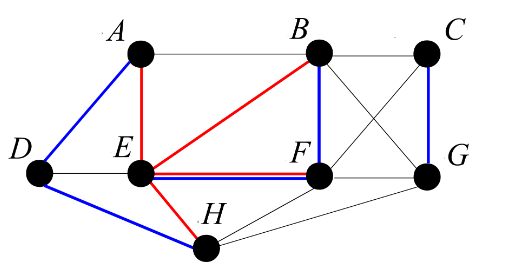
\includegraphics[width=0.6\columnwidth]{img/matroid1}
	\end{center}
	$$ x = \{(A, D) , (D, H) , (E , F ) , (B, F ) , (C , G )\} $$
	$$ y = \{(A, E ) , (B, E ) , (E , F ) , (E , H)\} $$
	$(A, D), (D, H)$ and $(C , G )$ can be added to $y$.\\
	
	\vfill
	
	\paragraph{TSP:} the first two axioms hold
	\begin{itemize}
		\item the empty set has no sub-tours and degrees $\leq 1$
		\item any proper subset of a set $\in F$ (no sub-tours and degrees $\leq 1$) also belongs to $F$
	\end{itemize}
	but the third axiom is violated.\\
	Example: $y = \{(1, 2), (2, 3)\}$ and $x = \{(3, 1), (1, 4), (4, 2)\}$.\\
	No arc of $x$ can be added to $y$ remaining in $F$.\\
	
	\newpage
	
	\subsubsection{Greedoids with the strong exchange axiom}
	The optimality of the greedy algorithm can be proved for greedoids (weaker second axiom) if the exchange axiom is strengthened.\\
	
	\textbf{Strong exchange axiom:}
	$$ 
	\begin{cases}
		x \in F, y \in B_F & \text{ such that } x \subset y \\
		i \in B \setminus y & \text{ such that } x \cup \left\{i\right\} \in F
	\end{cases}
	\implies \exists j \in y \setminus x: \, 
	\begin{cases}
		x \cup \left\{j\right\} \in F \\
		y \cup \left\{i\right\} \setminus \left\{j\right\} \in F
	\end{cases}
	$$
	
	Given a basis and one of its subsets (from which the basis is accessible), if there is an element that "leads astray" the subset from the base, there must be another one which keeps it on the right way and it must be feasible to exchange the two elements in the basis.\\
	
	Given a base $y$ and a subspace of the search space $x$, which is also a subset of the base, you can have an element $i$ not in $y$ that could be feasibly added to $x$. There must be another element inside $y$, but not $x$, that could be added to $x$ and replaced with $i$ in the base, all while remaining in the search space.\\
	
	\paragraph{MST:} A classical example of greedoid with strong exchange axiom is given by
	\begin{itemize}
		\item $B =$ edge set of a graph
		\item $F =$ collection of the trees including a given vertex $v_1$
	\end{itemize}
	that yields Prim’s algorithm for the MST problem.\\
	
	The trivial and the accessibility axiom hold (the heredity one does not).\\
	The exchange axiom holds in the strong form.\\
	
	\vfill
	
	\subsubsection*{Optimal constructive algorithms}
	Notice that the optimality of a constructive algorithm $A$ depends on
	\begin{itemize}
		\item the \textbf{properties of the problem} (e.g., additive objective function, bases as feasible solutions)
		\item the \textbf{properties of the search space} $F_A$ (that is, of the algorithm)
	\end{itemize}
	
	% End of L7
	
	\newpage
	
	\subsubsection{What to do when the axioms are violated}
	If a search space \textbf{violates} the desired \textbf{axioms}, one can try and \textbf{change} it.\\
	
	For the TSP, an alternative $F_A$ includes all paths starting from node $1$.\\
	Let $N_x$ be the set of nodes visited from $x$: the acceptable extensions are all arcs going out of the last node of path $x$ and not closing a sub-tour
	$$ \Delta_A^+ (x) = \left\{(h,k) \in A : \, h = \text{ Last } (x), \, k \notin N_x \text{ or } k = 1 \text{ and } N_x = N \right\} $$
	
	Unfortunately, the axioms are still not all satisfied
	\begin{itemize}
		\item the \textbf{trivial} axiom always \textbf{holds}
		\item the \textbf{accessibility} axiom \textbf{holds}: removing the last arc yields a path starting from node $1$
		\item the \textbf{heredity} axiom does \textbf{not hold}: not all subsets are paths
		\item the \textbf{exchange} axiom does \textbf{not hold}
	\end{itemize}
	
	Therefore, it is \textbf{not even a greedoid}.\\
	
	But the algorithm can still be a \textbf{reasonable heuristic}.\\
	
	\newpage
	
	\paragraph{The Nearest Neighbour heuristic for the TSP:} The Nearest Neighbour (NN) heuristic adopts the \textbf{alternative search space} keeping the \textbf{objective function} as the \textbf{selection criteria}
	\begin{enumerate}
		\item \textbf{Start} with an \textbf{empty set of arcs}: $x^{(0)} = \emptyset$ that represents a degenerate path going out of node $1$ (the optimal solution certainly visits node $1$).\\
		
		\item \textbf{Find} the \textbf{arc of minimum} cost going out of the last node of $x$
		$$ (i,j) = \arg \min_{(h,k \in \Delta_A^+ (x))} c_{hk} $$
		(the objective function is additive). It's selecting the "nearest neighbour", i.e. the next closest node, without closing a sub-tour (only unseen nodes).\\
		
		\item If $j \neq 1$, go back to point $2$; otherwise, terminate ($\Delta_A^+ (x)$ allows the return to node $1$ only at the last step).\\
	\end{enumerate}
	
	The algorithm is very intuitive, and its \textbf{complexity} is $\Theta (n^2)$ ($n$ iterations, $n$ time to choose the arc of minimum cost).\\
	
	It is not exact, but $\log n$-approximated (under the triangle inequality). You're going to find $\log n$ times the optimum, where $n$ is the number of nodes in the graph; it's not $\alpha$ approximated.\\
	
	\newpage
	
	\textbf{Example:} Consider a complete graph (the arcs are not reported for clarity)
	\begin{center}
		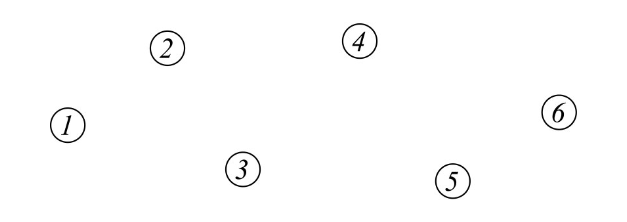
\includegraphics[width=0.5\columnwidth]{img/NNTSP1}
	\end{center}
	Starting from node 1 
	\begin{center}
		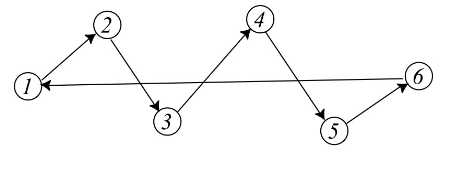
\includegraphics[width=0.5\columnwidth]{img/NNTSP2}
	\end{center}
	Starting from node 2
	\begin{center}
		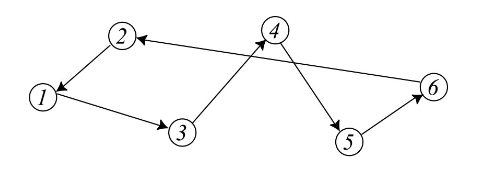
\includegraphics[width=0.5\columnwidth]{img/NNTSP3}
	\end{center}
	The optimal solution cannot be found starting from any node
	\begin{center}
		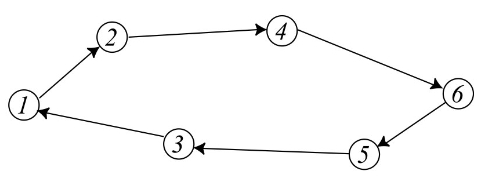
\includegraphics[width=0.5\columnwidth]{img/NNTSP4}
	\end{center}
	
	\newpage
	
	\subsection{Heuristic constructive algorithms (HCA): the KP}
	If the problem does \textbf{not admit} a \textbf{search space} with \textbf{suitable properties}, one must keep into account the \textbf{constraints of the problem} adopting
	\begin{enumerate}
		\item not only a \textbf{good definition} of $F_A$
		\item but also a \textbf{sophisticated definition of the selection criteria} $\varphi_A (i, x)$
	\end{enumerate}
	This allows effective results, even if not provably optimal.\\
	
	In the KP, the drawback derives from the volume of the objects: promising objects have a large value, but also a small volume
	\begin{itemize}
		\item define the \textbf{selection criteria} as the unitary value $\varphi_A (i, x) = \phi_i / v_i$ (getting the "value" of each piece to determine which is best)
	\end{itemize}
	
	The resulting algorithm
	\begin{itemize}
		\item can perform very badly
		\item with a small modification is 2-approximated
	\end{itemize}
	
	\vfill
	
	\paragraph{Example:}
	\begin{center}
		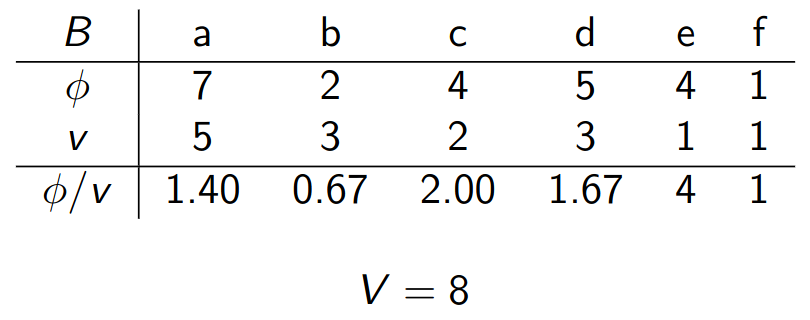
\includegraphics[width=0.5\columnwidth]{img/HKP1}
	\end{center}
	The algorithm performs the \textbf{following steps}:
	\begin{enumerate}
		\item $x := \emptyset$
		\item select $i := e$ and update $x := \{e\}$
		\item select $i := c$ and update $x := \{c, e\}$
		\item select $i := d$ and update $x := \{c, d, e\}$
		\item select $i := f$ and update $x := \{c, d, e, f \}$ (object $a$ does not fit)
		\item since $\Delta_A^+ (x) = \emptyset$, terminate
	\end{enumerate}
	The value of the solution found is $14$, the optimal solution is $x^\ast = \{a, c, e\}$ and its value is $15$. There can be critical cases with indefinitely bad gaps (it can discard large objects, even if they have large value).
	
	\newpage
	
	\subsubsection{2-Approximated algorithm for the KP}
	Steps
	\begin{enumerate}
		\item \textbf{Start} with an \textbf{empty subset}: $x^{(0)} = \emptyset$
		
		\item Find the \textbf{object} $i^{(t)}$ of \textbf{maximum unitary value} in $B \setminus x^{(t−1)}$:
		$$ i^{(t)} := \arg \max_{i \in B \setminus x^{(t-1)}} \frac{\phi_{i^{(t)}}}{v_{i^{(t)}}}$$
		it considers all elements, not only the one that respect the capacity.\\
		
		\item If it respects the capacity, \textbf{add} $i^{(t)}$ to $x^{(t−1)}$: $x^{(t)} := x^{(t−1)} \cup \{i^{(t)}\}$ and go \textbf{back to} point $2$.\\
		
		\item Build a \textbf{solution} with the \textbf{first rejected object}: $x' = \{i^{(t)}\}$.\\
		
		\item \textbf{Return the better solution} between $x$ and $x'$: $f_A = \max \left[f (x), f (x')\right]$.\\
	\end{enumerate}
	
	
	It is easy to prove that
	\begin{itemize}
		\item \textbf{the sum of the two solution values overestimates the optimum}
		$$ f(x) + f(x') = \sum_{\tau = 1}^{t} \phi_{i^{(\tau)}} \geq f^\ast $$
		This sum essentially represents a solution for a "bigger knapsack" (it exceeds the capacity), so it will obviously be better (upper bound).\\
		
		\item \textbf{the best of the two solution values is at least half their sum}
		$$ f_A = \max \left[ f(x), f(x')\right] \geq \frac{f(x) + f(x')}{2} \geq \frac{1}{2} f^\ast$$
		The larger one will obviously be more than half our earlier sum, which is larger than the optimal solution $\implies$ it will be larger than half the optimal solution.\\
	\end{itemize}
	
	\newpage
	
	\subsection{Pure and adaptive constructive algorithms}
	A constructive algorithm $A$ is
	\begin{itemize}
		\item \textbf{Pure} if the selection criteria $\varphi_A$ depends only on the new element $i$. The decision is made only on what to add, independently of the "past choices".\\
		
		\item \textbf{Adaptive} if $\varphi_A$ depends both on $i$ and on the current solution $x$.\\
	\end{itemize}
	
	Many criteria $\varphi_A (i, x)$ admit \textbf{equivalent forms} depending only on $i$
	\begin{itemize}
		\item In the TSP, $\varphi_A ((i, j), x) = f (x \cup \{(i, j)\})$ is equivalent to $c_{ij}$.\\
		
		\item In the KP, $\varphi_A (i, x) = f (x \cup \{i\})$ is equivalent to $\phi_i$
	\end{itemize}
	
	So far, we have seen only pure constructive algorithms.\\
	
	An \textbf{additive selection criteria} yields a \textbf{pure constructive algorithm}.\\
	
	\newpage
	
	\subsection{HCA: Set Covering}
	Given a binary matrix and a cost vector associated to the columns, find a minimum cost subset of columns covering all the rows (at least one $1$ for each row, choose columns, minimum cost).\\
	
	The \textbf{objective} is \textbf{additive}, but the solutions are \textbf{not maximal subsets} (actually, the smaller feasible subsets are better).\\
	
	An \textbf{adaptive selection criteria} $\varphi_A (i, x)$ is necessary: a pure one ($\varphi_A (i)$) could repeatedly choose columns covering the same rows.\\
	
	The more promising \textbf{ideas} are to consider
	\begin{itemize}
		\item the \textbf{objective function}: select columns of low cost
		\item the \textbf{constraints}: select columns covering many rows
		\item the \textbf{current subset} $x$: select columns covering new rows
	\end{itemize}
	
	In \textbf{summary}
	\begin{itemize}
		\item include in $\Delta_A^+ (x)$ only \textbf{columns covering additional rows} not in $x$
		\item apply the \textbf{adaptive selection criteria} $\varphi_A (i, x) = c_i / a_i (x)$ where $a_i (x)$ is the number of rows covered by $i$, but not by $x$. 
	\end{itemize}
	
	In the calculation we must take into account the columns we already covered, the selection criteria must consider only columns that have yet to be covered. This means that the algorithm must be adaptive, it can't be pure, otherwise it would choose "useless" columns.\\
	This is taken into account inside the definition of $a_i (x)$, which is defined as the number of rows covered by $i$, but not by $x$. \\
	
	\newpage
	
	\paragraph{Example:} this algorithm has the optimum as an upper bound, but it can also fail
	$$
	c \;\;\;\;
	\begin{array}{| c c c c c |}
		\hline
		25 & 6 & 8 & 24 & 12 \\
		\hline
	\end{array}
	$$
	
	$$
	A \;\;\;\;
	\begin{array}{| c c c c c |}
		\hline
		1 & 1 & 0 & 0 & 0 \\
		1 & 1 & 0 & 0 & 0 \\
		1 & 1 & 1 & 0 & 0 \\
		1 & 0 & 1 & 1 & 0 \\
		1 & 0 & 0 & 1 & 0 \\
		1 & 0 & 0 & 0 & 1 \\
		\hline
	\end{array}
	$$
	The algorithm performs the following \textbf{steps}:
	\begin{itemize}
		\item $x := \emptyset$
		\item since $c/a_i (x) = [4.1\overline{6}, \; 2, \; 4, \; 12, \; 12 ]$, select $i := 2$
		\item since $c/a_i (x) = [8.\overline{3}, \; -, \; 8, \; 12, \; 12 ],$ select $i := 3$
		\item since $c/a_i (x) = [12.5, \; -, \; -, \; 24, \; 12 ]$, select $i := 5$
		\item since $c/a_i (x) = [25, \; -, \; -, \; 24, \; - ]$, select $i := 4$
		\item all the rows are covered, therefore $\Delta_A^+ (x) = \emptyset$ and terminate
	\end{itemize}
	The solution returned is $x = \{2, 3, 4, 5\}$ and its value is 50, whereas the optimal solution $x^\ast = \{1\}$ has value $f^\ast = 25$.\\
	
	\newpage
	
	\subsubsection{Approximability of the SCP}
	This algorithm has a \textbf{non-constant} (logarithmic) \textbf{approximation ratio}
	\begin{itemize}
		\item At each step $t$, each column $i$ is evaluated with \textbf{criteria}
		$$ \varphi_A \left(i, x^{(t-1)}\right) = \frac{c_i}{a_i \left(x^{(t-1)}\right)} $$
		estimate of the unitary cost, cost of a column divided by the number of covered rows that are not already covered by the current solution.\\
		
		\item \textbf{Row} $j$ is \textbf{covered} by a certain \textbf{column} ($i_j$) at a certain \textbf{step} ($t_j$).\\
		
		\item Start assigning \textbf{weight} $\theta_j = 0$ to each \textbf{row} $j$.\\
		
		\item When each \textbf{row} $j$ is \textbf{covered} (step $t_j$), set its \textbf{weight} to
		$$ \theta_j = \frac{c_{i_j}}{a_{i_j} \left(x^{(t_j - 1)}\right)}$$
		so that the total weight of the rows increases by $c_{i_j}$ at step $t_j$; correspondingly, $x$ includes column $i_j$ and its cost increases by $c_{i_j}$.\\
		When you choose a column, put it in the partial solution and increase the cost of the solution by $c_{i_j}$, now modify the weights of the rows, take the cost of the column $c_{i_j}$ and divide it by how many new rows are covered, give each of these rows this increase in weight.\\
		
		\item The \textbf{total cost} of $x$ is always equal to the \textbf{total weight of the rows}
		$$ f_A (x) = \sum_{i \in x} c_i = \sum_{j \in R} \theta_j $$
		\nn
		
		\item at \textbf{step} $t$, there are $|R^{(t)}| \leq |R| − t$ \textbf{uncovered rows}.\\
		
		\newpage
		
		\item the columns of the optimal solution could cover them all with \textbf{cost} $f^\ast \implies$ at least one of such columns has \textbf{unitary cost} $\leq f^\ast /|R^{(t)}|$.\\
		
		\item the column $i$ selected has \textbf{minimum unitary cost} $\varphi_A (i, x^{(t−1)})$, therefore $\leq f^\ast /|R^{(t)}|$ and the covered rows \textbf{increase their weight} by
		$$ \theta_j = \varphi_A (i, x^{(t-1)}) \leq \frac{f^\ast}{|R^{(t_j)}|} \implies \sum_{j \in R} \theta_j \leq \sum_{j \in R} \frac{f^\ast}{|R^{(t_j)}|} $$
		The cost to cover each row $j$ is not larger than the optimum divided by the number of rows uncovered at the step in which $j$ gets covered.\\
		
		\item the integer number $|R^{(t)}|$ strictly \textbf{decreases} at each step.\\
		
		\item the sum can be \textbf{overestimated reducing} $|R^{(t)}|$ by $1$ at each step.\\
		
		\item The \textbf{approximation ratio} is limited by a \textbf{logarithmic guarantee}
		$$ f_A = \sum_{j \in R} \theta_j \leq \sum_{j \in R} \frac{f^\ast}{|R^{(t_j)}|} \leq \sum_{r=|R|}^1 \frac{f^\ast}{r} \leq \left(\ln |R| + 1\right) f^\ast $$
	\end{itemize}
	
	\newpage
	
	\subsection{HCA: Bin Packing Problem}
	Another adaptive problem, the BPP requires to divide a set $O$ of voluminous objects into the minimum number of containers of given capacity drawn from a set $C$.\\
	
	$B = O \times C$ includes the \textbf{object-container assignments} $(i, j)$
	\begin{itemize}
		\item with exactly \textbf{one container for each object}
		\item with the \textbf{total volume} in each container \textbf{not exceeding} the \textbf{capacity}
	\end{itemize}
	
	Let us define the \textbf{search space} $F_A$ as the set of \textbf{all partial solutions}.\\
	
	The \textbf{objective function} is a \textbf{bad selection criteria}, because it is flat.\\
	All the augmented subsets have the same value or increase it by $1$.\\
	
	\subsubsection{First-Fit heuristic}
	Consider the \textbf{object-container pairs} lexicographically
	\begin{itemize}
		\item \textbf{Start} with an \textbf{empty subset}: $x^{(0)} = \emptyset$
		\item \textbf{Select pair} $(i, j)$ according to the following criteria:
		\begin{itemize}
			\item $i$ is the \textbf{first} (minimum index) \textbf{unassigned object}
			\item $j$ is the \textbf{first container with enough residual capacity} for $i$ (a used container, if possible; an unused one otherwise)
		\end{itemize}
		\item \textbf{Add} the new \textbf{assignment} to the \textbf{solution}: $x^{(t)} := x^{(t−1)} \cup \{(i, j)\}$
	\end{itemize}
	
	Notice that the \textbf{choice} of $(i, j)$
	\begin{itemize}
		\item \textbf{does not minimize} $f (x \cup \{(i, j)\})$ (another $i$ could be better)
		\item is split into \textbf{two phases} (first $i$, then $j$)
	\end{itemize}
	
	Essentially, take each element and put it into the first container you find with enough space, used or otherwise.\\
	
	\newpage
	
	\paragraph{Example:}
	\begin{center}
		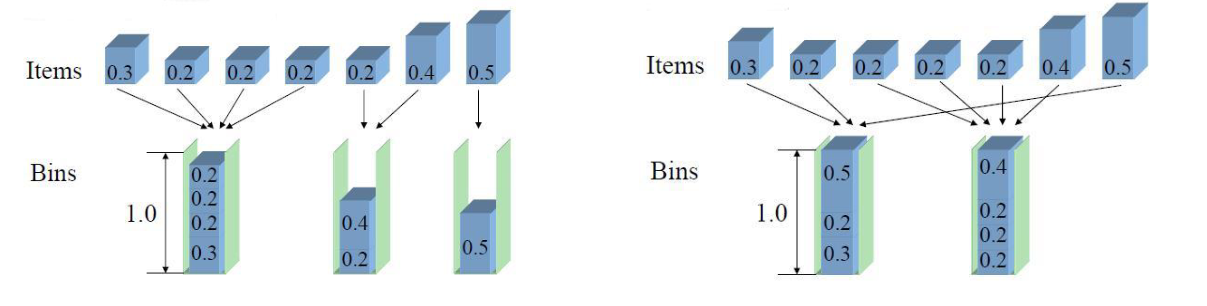
\includegraphics[width=\columnwidth]{img/CHBPP1}
	\end{center}
	\textbf{The solution is not optimal}; but it is \textbf{approximated}:
	\begin{itemize}
		\item At least $f^\ast \geq \sum_{i \in O} v_i / V$ \textbf{containers} are \textbf{necessary}. Lower bound, the minimum number of container if you could completely fill them all, it must be $\leq$ than the optimal solution.\\
		
		\item The \textbf{occupied volume} is $> V/2$ for \textbf{all used containers}, possibly except for the last one (if a second half-empty container existed, its objects would have been assigned to the first, it would be a contradiction).\\
		
		\item The \textbf{total volume exceeds} that of the $f_A − 1$ "saturated" containers
		$$ \sum_{i \in O} v_i > (f_A - 1)\frac{V}{2} $$
		This means that the total volume is more than $f_A - 1$ (if the last is not more than half full) times $V/2$ (lower bound).\\
		Which implies $(fA − 1) < 2/V \sum_{i \in O} v_i \leq 2f^\ast \implies f_A \leq 2f^\ast$. Our solution is less than the volume of the "saturated" containers expressed before, which in turn is smaller than the optimal solution, refactor the equation and we get the last part, our solution is less than twice the optimum $+1$.\\
		The analysis can be improved to 1.7.\\
	\end{itemize}
	
	\newpage
	
	\paragraph{Better choices?} The \textbf{approximation ratio} $\alpha = 2$ holds for \textbf{any permutation} of the objects.\\
	
	Intuition would suggest selecting first the smallest objects, in order to keep the objective $f (x \cup \{i\})$ as small as possible, but this neglects that all objects must be assigned.\\
	
	By contrast, it is \textbf{better to select the largest object first} because
	\begin{itemize}
		\item each object in a container has a volume strictly larger than the residual capacity of all the previous containers (otherwise, it would have been assigned to one of them)
		\item keeping the smallest objects in the end guarantees that many containers have a small residual capacity
	\end{itemize}
	This algorithm has a \textbf{better approximation ratio}: $f_A \leq (11/9) f^\ast + 1$.\\
	
	The difference is that instead of choosing the object of minimum index you choose the object of largest volume.\\
	
	% End of L8
	
	\newpage
	
	\subsection{Extensions of the basic constructive scheme}
	The \textbf{basic scheme} of constructive algorithms can be \textbf{enhanced} using
	\begin{enumerate}
		\item a \textbf{more effective construction graph}
		\begin{itemize}
			\item \textbf{add more than one element} to the current subset $x$
			\item add elements to $x$, but \textbf{also remove elements} from $x$ (without going back to visited subsets, otherwise the construction graph would be cyclic)
		\end{itemize}
		\nn
		
		\item a \textbf{more sophisticated selection criteria}, such as
		\begin{itemize}
			\item a \textbf{regret-based function} that estimates potential future losses associated with element $i$
			\item a \textbf{look-ahead function} that estimates the final value of the objective obtained adding $i$ to $x$
		\end{itemize}
	\end{enumerate}
	
	\newpage
	
	\subsubsection{Extensions of the construction graph}
	The constructive algorithm adds an element at a time to the solution.\\
	
	It is possible to \textbf{generalize} this scheme with algorithms that at each step
	\begin{enumerate}
		\item \textbf{Add more than one element:} the selection criteria $\varphi_A (B^+, x)$ identifies a subset $B^+ \subseteq B \setminus x$ to add, instead of a single element $i$. \\
		The criteria depends not only from $x$ but also on the subset of the ground set $B^+$.\\
		
		\item Add elements, but also \textbf{remove a smaller number of elements:} the selection criteria $\varphi_A (B^+, B^-, x)$ identifies a subset $B^+ \subseteq B \setminus x$ to add and a subset $B^- \subseteq x$ to remove, with $|B+| > |B-|$. \\
		The criteria becomes a function of $x$, $B^+$ and the subsets of element currently included in $x$ to remove $B^-$.\\
	\end{enumerate}
	
	These algorithms build an \textbf{acyclic construction graph} on the search space, so that they never revisit any subset.\\
	
	The fundamental problem is to \textbf{define a family} $\Delta_A^+ (x)$ of subset pairs such that \textbf{optimizing the selection criteria is a polynomial problem}
	$$ \min_{(B^+, B^-) \in \Delta_A^+ (x)} \varphi_A (B^+, B^-, x) $$
	that is
	\begin{itemize}
		\item subsets \textbf{efficiently optimizable} (minimum paths, ...)
		\item subsets of \textbf{limited size} (e.g., $|B^+| = 2$ and $|B^-| = 1$)
	\end{itemize}
	
	Minimizing the selection criteria can become difficult, there could be exponentially many subsets. To counteract that we can limit the size of our subsets $B^+$ and $B^-$ or define specific families for these subsets such that they are "classic problems" and consequently easily optimizable (e.g. minimum paths).\\
	
	\newpage
	
	\subsection{The Steiner Tree Problem (STP)}
	Given an undirected graph $G = (V , E )$, a cost function $c : E \rightarrow \mathbb{N}$ on the edges and a subset of special vertices $U \subset V$, find a tree connecting at minimum cost all special vertices.
	\begin{center}
		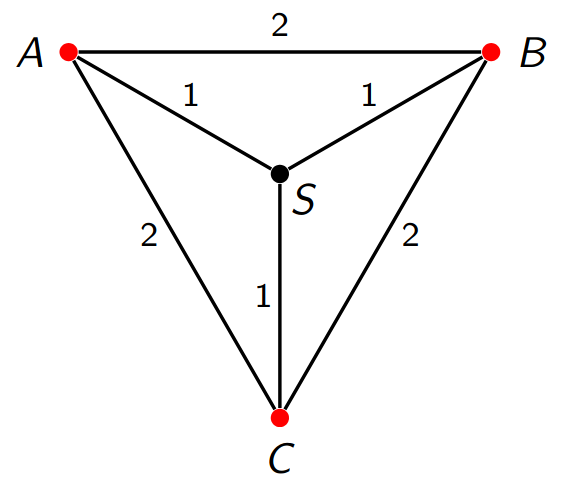
\includegraphics[width=0.6\columnwidth]{img/STP1}
	\end{center}
	The minimum tree spanning the special vertices is not necessarily optimal (and it might not even exist).\\
	
	Basically, connect the special dots and make it quick.\\
	
	\newpage
	
	\subsubsection{Distance Heuristic (DH) for the STP}
	A basic constructive algorithm could adopt the same \textbf{search spaces} as
	\begin{itemize}
		\item Kruskal's algorithm: the set of \textbf{all forests}
		\item Prim's algorithm: the set of \textbf{all trees including a (special) vertex}
	\end{itemize}
	
	but adding \textbf{one edge at a time}
	\begin{itemize}
		\item returns solutions with \textbf{redundant edges}, therefore expensive
		\item has a hard time \textbf{distinguishing useful and redundant} edges
	\end{itemize}
	
	The Distance Heuristic adopts as \textbf{search space} $F$ the \textbf{collection of all trees including a given special vertex} $v_1$ (as in Prim).\\
	
	It iteratively \textbf{adds a path} $B^+$ \textbf{between} $x$ \textbf{and a special vertex} instead of a single edge, so that
	\begin{itemize}
		\item $x$ \textbf{remains a tree}
		\item $x$ \textbf{spans a new special vertex}
		\item the \textbf{minimum cost path} can be \textbf{computed efficiently} at each step
	\end{itemize}
	
	It \textbf{terminates} when \textbf{all special vertices are connected}.\\
	
	Instead of adding only one edge at a time, at each step it adds the minimum cost path from an already visited vertex (not necessarily special) to the next closest special vertex, keeping the solution less redundant and simplifying the computation of the minimum cost path.\\
	
	\newpage
	
	\paragraph{Example:}
	\begin{center}
		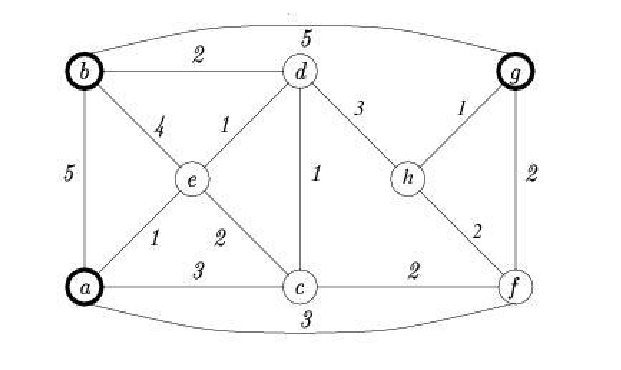
\includegraphics[width=0.7\columnwidth]{img/STP2}
	\end{center}
	
	\begin{itemize}
		\item Start with a single special vertex $a$: $x := \emptyset$ (degenerate tree).\\
		
		\item Add the closest special vertex ($b$) through path $(a, e, d, b)$:
		$$ x = \{(a, e) , (e, d) , (d, b)\} $$
		
		\item Add the closest special vertex ($g$) through path $(g , h, d)$:
		$$ x = \{(a, e) , (e, d) , (d, b) , (g , h) , (h, d)\} $$
		The Distance Heuristic algorithm is 2-approximated: it is equivalent to computing a minimum spanning tree on a graph with
		\begin{itemize}
			\item vertices reduced to the special vertices
			\item edges corresponding to the minimum paths
		\end{itemize}
		You can think of it as a graph with only special vertices and the minimum path between them as edges.\\
		
		\item All special vertices are in the solution: terminate (this time the solution is optimal)
	\end{itemize}
	
	\newpage
	
	\paragraph{Counterexample to optimality:} Consider a complete graph $G = (V , E )$ with $U = V \setminus \{1\}$ and cost
	$$ 
	c_{uv} = \begin{cases}
		(1 + \epsilon)M & \text{ for } u \text{ or } v = 1 \\
		2M & \text{ for } u,v \in U
	\end{cases}
	$$
	($M$ is just used to obtain integer costs for any $\epsilon$).\\
	Every arc from node 1 cost $(1 + \epsilon)M$, $2M$ for everything else.\\
	
	The DH returns a star spanning the special vertices: $f_{DH} = (n − 2) \cdot 2M$.\\
	
	The optimal solution is a spanning star centered in $1$: $f^\ast = (n − 1) \cdot (1 + \epsilon)M$.
	
	\begin{center}
		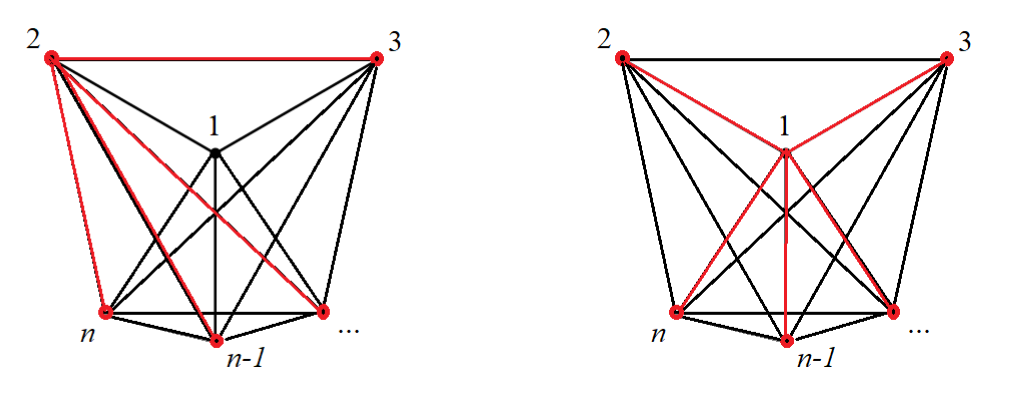
\includegraphics[width=0.9\columnwidth]{img/STP3}
	\end{center}
	
	The approximation ratio is 
	$$ \rho_{DH} = \frac{f_{DH}}{f^\ast} = \frac{n-2}{n-1} \cdot \frac{2}{1 + \epsilon} < 2 $$
	and converges to $2$ as $n$ increases and $\epsilon$ decreases.\\
	
	\newpage
	
	\subsection{Insertion algorithms for the TSP}
	Several heuristic algorithms for the TSP define the \textbf{search space} $F_A$ as the \textbf{set of all circuits} of the graph \textbf{including a given node}; a circuit
	\begin{itemize}
		\item \textbf{cannot} be obtained from another one by \textbf{adding a single arc}
		\item \textbf{can} be obtained \textbf{adding two arcs} $(i, k)$, $(k, j)$ and \textbf{removing one} $(i, j)$
	\end{itemize}
	
	\begin{center}
		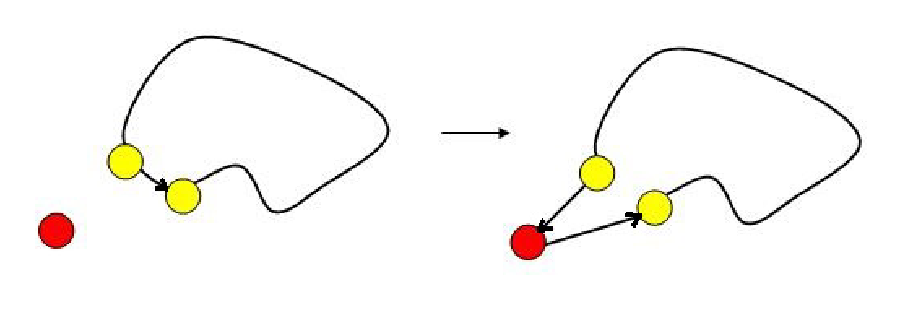
\includegraphics[width=0.8\columnwidth]{img/IATSP1}
	\end{center}
	
	Steps
	\begin{enumerate}
		\item Start with a \textbf{zero-cost self-loop on node} $1$: $x^{(0)} = \{(1, 1)\}$ (Not much different from an \textbf{empty set})
		
		\item Select a \textbf{node} $k$ to be \textbf{added} and an \textbf{arc} $(i, j)$ to be \textbf{removed}
		
		\item If the circuit \textbf{does not visit all nodes}, go back to point $2$; \textbf{otherwise terminate}
	\end{enumerate}
	
	Such a scheme \textbf{never visits again the same solution} and builds a \textbf{feasible solution in} $n - 1$ steps (each step adds a new node).\\
	
	Start from a circuit, add one node at a time by adding a new edge and removing an old one.\\
	
	\newpage
	
	\subsubsection{Cheapest Insertion heuristic} 
	The selection criteria $\varphi_A (B^+, B^-, x)$ must \textbf{choose an arc and a node}; there are $(n − |x|) |x| \in O (n^2)$ alternatives
	\begin{itemize}
		\item $|x|$ possible \textbf{arcs} ($s_i , s_{i+1}$) to \textbf{remove}; the nodes already in the circuit
		\item $n − |x|$ possible \textbf{nodes} $k$ to \textbf{add} through the arcs ($s_i , k$) and ($k, s_{i+1}$); nodes not yet in the circuit that can be added
	\end{itemize}
	
	The \textbf{Cheapest Insertion} (CI) heuristic uses as a \textbf{selection criteria}
	$$ \varphi_A (B^+, B^-, x) = f \left(x \cup B^+ \setminus B^- \right) $$
	
	\textbf{Objective function} $f (x)$ is \textbf{additive}, hence \textbf{extensible} to the whole of $F_A$.\\
	
	Here $k$ denotes a general node outside the circuit, $s_i$ (or anything $s$-related) denotes nodes already inside the circuit.\\
	
	Since $f (x \cup B^+ \setminus B^-) = f (x) + c_{s_i ,k} + c_{k,s_{i+1}} - c_{s_i ,s_{i+1}}$ (objective function $+$ the cost of the arcs added $-$ the cost of the arc removed)
	$$ \arg \min_{B^+, B^-} \varphi_A \left(B^+, B^-, x \right) = \arg \min_{i,k} (c_{s_i, k} + c_{k, s_{i+1}} - c_{s_i, s_{i+1}})$$
	We need to minimize these terms by choosing the set of $i,k$ that minimizes the variation in cost. \\
	
	The \textbf{computational cost of evaluating} $\varphi_A$ \textbf{decreases} from $\Theta (n)$ to $\Theta (1)$ (since we need to compute only the variation).\\
	
	\newpage
	
	\paragraph{Algorithm Cheapest Insertion:}
	\begin{enumerate}
		\item Start with a \textbf{zero-cost self-loop} on node $1$: $x^{(0)} = \{(1, 1)\}$. It is also like starting with a single node.
		
		\item Select the \textbf{arc} $(s_i , s_{i+1}) \in x$ and the \textbf{node} $k \notin N_x$ \textbf{such that} ($c_{s_i, k} + c_{k, s_{i+1}} − c_{s_i ,s_{i+1}}$) is minimum; select the node to add and the arc to remove, such that the total variation is at a minimum.
		
		\item If the circuit does not visit all nodes, go back to point $2$; otherwise terminate.
	\end{enumerate}
	It is not exact, but \textbf{2-approximated}, under the triangle inequality.\\
	
	The CI algorithm performs $n - 1$ steps: at each step $t$
	\begin{itemize}
		\item it evaluates $(n - t) t$ node-arc pairs
		\begin{itemize}
			\item each evaluation requires constant time
			\item each evaluation possibly updates the best move
		\end{itemize}
		\item it performs the best addition/removal
		\item it decides whether to terminate
	\end{itemize}
	
	The \textbf{overall complexity} is $\Theta (n^3)$.\\
	
	It can be reduced to $\Theta (n^2 \log n)$ collecting in a min-heap the insertion costs for each external node: each of the $n$ steps
	\begin{itemize}
		\item selects the best insertion in $O (n)$ time and performs it
		\item creates two new insertions and removes one for each external node, and updates their heaps in $O (n \log n)$ time
	\end{itemize}

	\newpage
	
	\subsubsection{Nearest Insertion heuristic}
	The algorithm Cheapest Insertion tends to select nodes close to circuit $x$: minimizing $c_{s_i ,k} + c_{k,s_{i+1}} - c_{s_i ,s_{i+1}}$ implies that $c_{s_i ,k}$ and $c_{s_{i+1},k}$ are small (looks for the closest node to add, the weight of the arcs to that node must be small).\\
	
	To accelerate, one can \textbf{decompose criteria} $\varphi_A$ \textbf{into two phases}.\\
	
	\paragraph{Algorithm Nearest Insertion (NI):}
	\begin{enumerate}
		\item start with a \textbf{zero-cost self-loop} on node $1$: $x^{(0)} = \{(1, 1)\}$
		
		\item \textbf{Add criteria:} select the \textbf{node} $k$ \textbf{nearest to circuit} $x$
		$$ k = \arg \min_{l \notin N_x} \left(\min_{s_i \in N_x} c_{s_i, l} \right) $$
		It chooses the minimum distance among the minimum distances of each node from the circuit.
		
		\item \textbf{Delete criteria:} select the \textbf{arc} ($s_i , s_{i+1}$) that \textbf{minimizes} $f$
		$$ (s_i, s_{i+1}) = \arg \min_{s_i, s_{i+1} \in x} \left(c_{s_i, k} + c_{k, s_{i+1}} - c_{s_i, s_{i+1}}\right) $$
		The arc to break is the one that minimizes the objective function.
		
		\item If the circuit does not visit all nodes, go back to point 2; otherwise terminate
	\end{enumerate}
	
	It is not exact, but \textbf{2-approximated}, under the triangle inequality.\\
	
	Instead of choosing together node and arc, you first choose the node and, given the node, the arc is chosen; you look for the node closest to the circuit in general. \\
	Instead of minimizing the new cost, the cost of the arc that connects the new node to the circuit is minimized.\\
	
	\newpage
	
	The NI algorithm performs $n - 1$ steps: at each step $t$ it
	\begin{itemize}
		\item \textbf{Evaluates the distance} of $(n - t)$ nodes from the circuit (the remaining nodes), each one in $\Theta (t)$ time (confront them with the nodes already in the circuit); it makes this $\Theta (n^2)$.\\
		
		\item \textbf{Selects} the \textbf{node at minimum distance}.\\
		
		\item \textbf{Evaluates the removal} of $t$ arcs, each one in $\Theta (1)$ time.\\
		
		\item Performs the \textbf{best addition/removal}.\\
		
		\item \textbf{Decides} whether to \textbf{terminate}.\\
	\end{itemize}
	
	The \textbf{overall complexity} is $\Theta (n^3)$.\\
	
	It \textbf{can be reduced to} $\Theta (n^2)$ collecting in a vector for each external node the closest internal node: each of the $n - 1$ steps
	\begin{itemize}
		\item selects the closest node in $O (n)$ time
		\item finds the insertion point in $O (n)$ time
		\item inserts the node creating a new internal node for each external node, which possibly becomes the closest saved in the vector; each of the $O (n)$ updates takes $O (1)$ time
	\end{itemize}
	
	It has the same approximation guarantee as the last heuristic, but it's faster.\\
	
	\newpage
	
	\subsubsection{Farthest Insertion heuristic}
	The choice of the closest node to the cycle is natural, but misleading: since all nodes must be visited, it is preferable to service in the best way the most problematic ones (i.e., the farthest ones).\\
	
	\paragraph{Algorithm Farthest Insertion (FI):}
	\begin{enumerate}
		\item Start with a \textbf{zero-cost self-loop} on node $1$: $x^{(0)} = \{(1, 1)\}$.\\
		
		\item \textbf{Add criteria:} select the node $k$ \textbf{farthest} from cycle $x$
		$$ k = \arg \max_{l \notin N_x} \left(\min_{s_i \in N_x} c_{s_i, l}\right) $$
		(the node that is farthest from the closest node of the cycle) the maximum of the minimum distances from the circuit.\\
		
		\item \textbf{Delete criteria:} select the arc ($s_i , s_{i+1}$) minimizing
		$$ (s_i, s_{i+1}) = \arg \min_{(s_i, s_{i+1} \in x} \left(c_{s_i, k} + c_{k, s_{i+1}} - c_{s_i, s_{i+1}} \right) $$
		
		\item If the circuit does not visit all nodes, go back to point 2; otherwise terminate.\\
	\end{enumerate}
	
	It is \textbf{$\log n$-approximated} under the triangle inequality, hence \textbf{worse} than the previous ones in the \textbf{worst-case} (but often \textbf{experimentally better}).\\
	
	\newpage
	
	It starts by inserting the furthest possible nodes (but includes them in the best way), until it forms a complete circuit. This way the "isolated" nodes can be connected first and penalize less the final result.\\
	
	The FI algorithm performs $n - 1$ steps: at each step $t$
	\begin{itemize}
		\item it \textbf{evaluates the distance} of $(n - t)$ nodes from the circuit, each one in $\Theta (t)$ time
		\item \textbf{select} the node at \textbf{maximum distance}
		\item it \textbf{evaluates the removal} of $t$ arcs, each one in $\Theta (1)$ time
		\item it performs the \textbf{best addition/removal}
		\item it \textbf{decides} whether to \textbf{terminate}
	\end{itemize}
	
	The complexity is the same as the NI (just with the farthest).\\
	
	The overall complexity is $\Theta (n^3)$.\\
	
	It can be reduced to $\Theta (n^2)$ as in the NI heuristic.\\
	
	\newpage
	
	\subsection{Regret-based constructive heuristics}
	We've seen how to make a more effective construction graph, the other method to extend a constructive algorithm is a more sophisticated selection criteria, such as a look-ahead or regret-based function.\\
	
	\textbf{Decisions taken in early steps can severely restrict the feasible choices} in later steps due to the \textbf{constraints} of the problem
	\begin{itemize}
		\item \textbf{BPP:} all objects must be put into a container, but early assignments could make some containers unavailable for later objects
		
		\item \textbf{TSP:} all nodes must be visited, but early routing decisions could make the visit of later nodes more expensive (even impossible, if the graph is noncomplete)
		
		\item \textbf{CMST:} all vertices must be linked to the root through a subtree, but early links could make some subtrees unavailable for later vertices
	\end{itemize}
	
	The selection criteria can take it into account \textbf{implicitly}
	\begin{itemize}
		\item \textbf{BPP:} the Decreasing First-Fit heuristic assigns the larger objects first
		\item \textbf{TSP:} the Farthest Insertion heuristic visits the farther nodes first
	\end{itemize}
	
	Some selection criteria aim explicitly to \textbf{leave larger sets of good choices}.\\
	
	\paragraph{Regret criteria:} A typical regret-based heuristic consists in
	\begin{itemize}
		\item \textbf{partitioning} $\Delta_A^+ (x)$ into disjoint classes of choices (the assignments of each object, how every object can be assigned, the edges incident in each vertex)
		
		\item compute a \textbf{basic selection criteria} for all choices
		
		\item compute \textbf{for each class the regret}, i.e. the \textbf{difference} between either
		\begin{itemize}
			\item the \textbf{second-best choice} or
			\item the \textbf{average of the other choices} (possibly weighted)
		\end{itemize}
		and the best choice in order to estimate the damage incurred by postponing the best choice until it becomes impossible
		
		\item \textbf{choose} the \textbf{best choice} of the class for which the \textbf{regret is maximum}. This is effective when a single choice per class must be taken
	\end{itemize}
	
	Essentially we divide the possible additions into classes (for example all the feasible assignments of an object is a single class), and pick the (greedy) best choice for each class. To choose from which class to pick the best choice, we use the regret, maximizing it.\\
	
	The regret represents how much worse the other choices will be, so we choose the best choice of the class with the highest regret, "fearing" that if we don't pick that option now, we'll be forced to pick a much worse one later on. \\
	
	You can make this reasoning when you're sure that you will have to take at least one choice for each class.\\
	
	\paragraph{Example:} Consider the CMSTP and ground set $B = V \times T$ (($vertex,subtree$) pairs). Let the weights be uniform ($w_v = 1$ for all $v \in V$) and capacity $W = 2$
	
	\begin{center}
		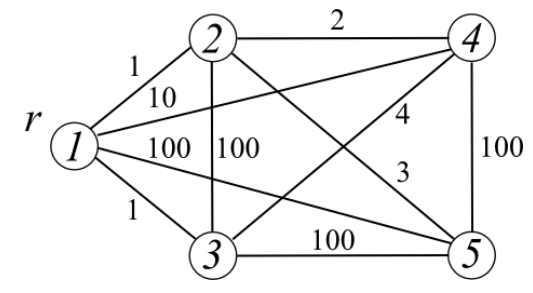
\includegraphics[width=0.5\columnwidth]{img/RBCSMTP}
	\end{center}
	
	Let the search space $F$ include all partial solutions.\\
	
	The greedy algorithm puts vertex $2$ in subtree $1$, vertex $3$ in subtree $2$; then vertex $4$ in subtree $1$ and finally vertex $5$ in subtree $3$:
	$$ c(x) = 1 + 1 + 2 + 100 = 104$$ 
	
	The regret algorithm puts vertex $2$ in subtree $1$, vertex $3$ in subtree $2$; now:
	\begin{itemize}
		\item the regret of vertex $3$ is the difference $c(3, 3) − c(3, 2) = 1 − 1 = 0$
		\item the regret of vertex $4$ is the difference $c(4, 2) − c(4, 1) = 10 − 2 = 8$
		\item the regret of vertex $5$ is the difference $c(5, 2) − c(5, 1) = 100 − 3 = 97$
	\end{itemize}
	The algorithm puts vertex $5$ in subtree $1$.\\
	Then, it proceeds putting vertices $2$ and $4$ in subtree $2$:
	$$ c(x) = 1 + 3 + 1 + 4 = 9 $$
	
	\newpage
	
	\subsection{Roll-out heuristics}
	They are also known as \textbf{single-step look-ahead constructive heuristics} and were proposed by Bertsekas and Tsitsiklis (1997).\\
	
	Given a \textbf{basic constructive heuristic} $A$
	\begin{itemize}
		\item \textbf{start} with an \textbf{empty subset}: $x^{(0)} = \emptyset$
		
		\item at each step $t$
		\begin{itemize}
			\item \textbf{extend} the \textbf{subset} in \textbf{each feasible way}: $x^{(t−1)} \cup \{i\}$, $\forall i \in \Delta_A^+ (x)$
			
			\item \textbf{apply} the \textbf{basic heuristic} to \textbf{each extended subset} and compute the resulting solution $x_A (x^{(t−1)} \cup \{i\})$
			
			\item use the \textbf{value of the solution} as the \textbf{selection criteria} to choose $i^(t)$
			$$ \varphi_A (i,x) = f \left(x_A \left(x^{(t-1)} \cup \left\{i\right\} \right) \right)$$
		\end{itemize}
		
		\item \textbf{terminate} when $\Delta_A^+ (x)$ is empty
	\end{itemize}
	
	Try every feasible move, look at the result, go back and choose the move. \\
	
	The \textbf{result} of the roll-out heuristic \textbf{dominates that of the basic heuristic} (under very general conditions). I'm trying every possibility, of course it's going to be better.\\
	
	The \textbf{complexity remains polynomial}, but is \textbf{much larger} (I have to run the algorithm many more times): in the worst case, $T_{ro(A)} = |B|^2 T_A$.\\
	
	The basic complexity is multiplied by the dimension of the ground set squared, because at each point you have to make several attempts and for each one run the algorithm ("standard" complexity times the number of attempts).\\
	
	\newpage
	
	\paragraph{Example:} roll-out for the SCP
	$$
	c \;\;\;\;
	\begin{array}{| c c c c c |}
		\hline
		25 & 6 & 8 & 24 & 12 \\
		\hline
	\end{array}
	$$
	
	$$
	A \;\;\;\;
	\begin{array}{| c c c c c |}
		\hline
		1 & 1 & 0 & 0 & 0 \\
		1 & 1 & 0 & 0 & 0 \\
 		1 & 1 & 1 & 0 & 0 \\
		1 & 0 & 1 & 1 & 0 \\
		1 & 0 & 0 & 1 & 0 \\
		1 & 0 & 0 & 0 & 1 \\
		\hline
	\end{array}
	$$
	
	\begin{enumerate}
		\item start with the empty subset: $x^{(0)} = \emptyset$
		
		\item for each column $i$, apply the constructive heuristic starting from subset $x^{(0)} \cup \{i\} = \{i\}$
		\begin{itemize}
			\item for $i = 1$, obtain $x_A (\{1\}) = \{1\}$ of cost $f_A (\{1\}) = 25$
			\item for $i = 2$, obtain $x_A (\{2\}) = \{2, 3, 5, 4\}$ of cost $f_A (\{2\}) = 50$
			\item for $i = 3$, obtain $x_A (\{3\}) = \{3, 2, 5, 4\}$ of cost $f_A (\{3\}) = 50$
			\item for $i = 4$, obtain $x_A (\{4\}) = \{4, 2, 5\}$ of cost $f_A (\{4\}) = 43$
			\item for $i = 5$, obtain $x_A (\{5\}) = \{5, 2, 3, 4\}$ of cost $f_A (\{5\}) = 50$
		\end{itemize}
		It tries every possible solution (in this case "fixing" a starting column)
		
		\item the best solution is the first one, therefore $i^{(1)} = 1$
		
		\item all rows are covered: the algorithm terminates
	\end{enumerate}
	
	\newpage
	
	\subsubsection{Generalized roll-out heuristics}
	The scheme can be \textbf{generalized}
	\begin{itemize}
		\item \textbf{applying several basic heuristics} $A^{[1]}, \, ... \, , A^{[l]}$
		
		\item \textbf{increasing the number of look-ahead steps}, i.e., using $x^{(t−1)} \cup B^+$ with $|B^+| > 1$ (add more than one element and check all possibilities)
	\end{itemize}
	
	The \textbf{result improves} and the \textbf{complexity worsens} further.\\
	
	The overall scheme does not change significantly
	\begin{itemize}
		\item start from the empty subset: $x^{(0)} = \emptyset$
		
		\item at each step $t$
		\begin{itemize}
			\item for each possible extension $B^+ \in \Delta_A^+ (x^{(t−1)})$ apply each basic algorithm $A^{[l]}$ starting from $x^{(t−1)} \cup B^+$
			
			\item the selection criteria is $\min_l f_{A^{[l]}} (x^{(t−1)} \cup B^+)$
			
			\item use the value of the best solution as the selection criteria for $i^{(t)}$
			$$ \varphi_A (i,x) = \min_{L = 1, \, ... \, , l} f \left(x_A \left(x^{(t-1)} \cup \left\{i\right\} \right) \right) $$
		\end{itemize}
		\item when $\Delta_A^+ (x)$ is empty, terminate
	\end{itemize}
	
	\newpage
	
	\subsection{Destructive heuristics}
	It is an approach exactly complementary to the constructive one
	\begin{itemize}
		\item \textbf{Start} with the \textbf{full ground set}: $x^{(0)} := B$.\\
		
		\item \textbf{Remove an element at a time}, selected 
		\begin{itemize}
			\item so as to \textbf{remain within the search space} $F_A$
			$$ \Delta_A^+ (x) = \left\{i \in x : \, x \setminus \left\{i\right\} \in F_A \right\} $$
			
			\item \textbf{maximizing the selection criteria} $\varphi_A (i, x)$ (usually a cost reduction)
		\end{itemize}
		\nn
		
		\item \textbf{Terminate} when $\Delta_A^+ (x) = \emptyset$ (there is no way to remain in $F_A$)
	\end{itemize}
	
	
	A destructive heuristic (for a minimization problem) can be described as
	\begin{algorithm}
		\caption{Algorithm $Stingy(I)$}
		\begin{algorithmic}
			\STATE $x := B$; $x^\ast := B$
			\IF{$x \in X$}
				\STATE $f^\ast := f (x)$ 
			\ELSE 
				\STATE $f^\ast := + \infty$ù
			\ENDIF
			\WHILE{$\Delta_A^+ (x) \neq \emptyset$}
				\STATE $i := \arg \max_{i \in \Delta_A^+ (x)} \varphi_A (i,x)$
				\STATE $x := x \setminus \left\{i\right\}$
				\IF{$x \in X$ and $f(x) < f^\ast$}
					\STATE $x^\ast := x$
					\STATE $f^\ast := f(x)$
				\ENDIF
			\ENDWHILE
			\RETURN ($x^\ast, f^\ast$)
		\end{algorithmic}
	\end{algorithm}
	Optimal for the Minimum Spanning Tree Problem.\\
	
	Essentially this is "throwing away" the most expensive edges one at a time, without forming a disconnected graph.\\
	
	\newpage
	
	\paragraph{Why are they less used?} When the \textbf{solutions are much smaller than the ground set} ($|x| \ll |B|$) a destructive heuristic
	\begin{itemize}
		\item requires a \textbf{larger number of steps}
		
		\item is \textbf{more likely} to \textbf{make a wrong decision} at an early step
		
		\item sometimes \textbf{requires more time to evaluate} $\Delta_A^+ (x)$ and $\varphi_A (i, x)$
	\end{itemize}
	
	When a \textbf{constructive heuristic returns redundant solutions}, it is useful to \textbf{append a destructive heuristic} at its end as a post-processing phase.\\
	
	This auxiliary destructive heuristic
	\begin{itemize}
		\item \textbf{starts from the solution} $x$ of the constructive heuristic, instead of $B$
		
		\item adopts as a \textbf{search space} the \textbf{feasible region}:
		$$ F_A = X \implies \Delta_A^+ (x) = \left\{ i \in x : \, x \setminus \left\{i\right\} \in X \right\} $$
		
		\item adopts as the \textbf{selection criteria} the \textbf{objective function}:
		$$ \varphi_A (i,x) = f (x \setminus \left\{i\right\}) $$
		
		\item \textbf{terminates after very few steps}
	\end{itemize}
	
	\newpage
	
	\paragraph{Constructive/destructive heuristic example for the SCP:}
	$$
	c \;\;\;\; 
	\begin{array}{| c c c c |}
		\hline
		6 & 8 & 24 & 12 \\
		\hline
	\end{array}
	$$
	
	$$
	A \;\;\;\;
	\begin{array}{| c c c c |}
		\hline 
		1 & 0 & 0 & 0 \\
		1 & 0 & 0 & 0 \\
		1 & 1 & 0 & 0 \\
		0 & 1 & 1 & 0 \\
		0 & 0 & 1 & 0 \\
		0 & 0 & 0 & 1 \\
		\hline 
	\end{array}
	$$
	
	\begin{enumerate}
		\item The constructive heuristic selects, in order, columns $1, 2, 4$ and $3$ (each one covers new rows).\\
		
		\item The solution is redundant: column $2$ can be removed (the following columns also cover already covered rows).\\
		
		\item The auxiliary destructive heuristic removes column $2$ and provides the optimal solution $x^\ast = \{1, 3, 4\}$ (columns $1, 3$ and $4$ are essential to cover rows $1, 2, 5$ and $6$).\\
	\end{enumerate}
	
	\newpage
	
	\subsection*{Summary about constructive and destructive algorithms}
	\addcontentsline{toc}{subsection}{Summary about constructive and destructive algorithms}
	
	Constructive and destructive algorithms
	\begin{enumerate}
		\item Are \textbf{intuitive}.\\
		
		\item Are \textbf{simple to design, analyze and implement}.\\
		
		\item Are \textbf{very efficient} (low-order polynomials)
		$$ T_A (n) \in O \left(T_{\Delta_A^+} (n) + T_{\varphi_A} (n) \right) $$
		where
		\begin{itemize}
			\item $T_{\Delta_A^+} (n)$ is the cost to identify $\Delta_A^+ (x)$
			
			\item $T_{\varphi_A} (n)$ is the cost to evaluate $\varphi_A (i,x)$ for each $i \in \Delta_A^+ (x)$
			
			\item the selection of $\arg \min \varphi_A (i, x)$ and update of $x$ (and auxiliary data structures) are dominated
		\end{itemize}
		\nn
		
		\item Have a \textbf{strongly variable effectiveness}
		\begin{itemize}
			\item on some problems they guarantee an optimal solution
			\item on other problems they provide an approximation guarantee
			\item on most problems they provide solutions of extremely variable quality, often scarce
			\item on some problems they cannot even guarantee a feasible solution
		\end{itemize}
		\nn
	\end{enumerate}
	
	It is fundamental to \textbf{study the problem before the algorithm}.\\
	
	\paragraph{When are they used?} Constructive and destructive algorithm are used
	\begin{enumerate}
		\item when they provide the optimal solution
		
		\item when the execution time must be very short (e.g., for on-line problems: schedulers, on-call services, ...)
		
		\item when the problem has a huge size or requires heavy computations (e.g., some data are obtained by simulation)
		
		\item as component of other algorithms, for example as
		\begin{itemize}
			\item starting phase for exchange algorithms
			\item basic procedure for recombination algorithms
		\end{itemize}
	\end{enumerate}
	
	% End of L9
	% L10 is lab, so the next is L11
	
	\section{Constructive Metaheuristics}
	
	The constructive algorithms have strong limitations on many problems. What can be done, without abandoning the general scheme? \\
	
	\textbf{Iterate the scheme} to generate many (potentially) \textbf{different solutions}:
	\begin{itemize}
		\item the \textbf{efficiency decreases}: the computational times are summed
		\item the \textbf{effectiveness increases}: the best solution is returned
	\end{itemize}
	
	The trade-off must be carefully tuned.\\
	
	The iterated scheme can apply
	\begin{itemize}
		\item \textbf{multi-start}, that is \textbf{different algorithm} at \textbf{each iteration} $l = 1,\, ... \, , \ell$ (this requires to define multiple $\mathcal{F}_{A_l}$ and $\varphi_{A_l}$)
	\end{itemize}
	
	but it is more flexible to apply \textbf{metaheuristics}, that exploit
	\begin{itemize}
		\item \textbf{randomization} (operations based on a random seed), as in the case of semigreedy algorithms, \textit{GRASP} and \textit{Ant System} (partly, \textit{ART})
		
		\item \textbf{memory} (operations based on the solutions of previous iterations), as in the case of \textit{ART}, cost perturbation and \textit{Ant System}
	\end{itemize}
	
	\paragraph{Termination condition:} The iterated scheme can ideally proceed for an infinite time.\\
	In pratice, one uses termination conditions that can be "absolute"
	
	\begin{enumerate}
		\item a given \textbf{total number of iterations} of the basic scheme
		
		\item a given \textbf{total execution time}
		
		\item a given \textbf{target value of the objective}
	\end{enumerate}
	
	or "relative" to the profile of $f^\ast$
	\begin{enumerate}
		\item a given \textbf{number of iterations} of the basic scheme \textbf{without improving} $f^\ast$
		
		\item a given \textbf{execution time without improving} $f^\ast$
		
		\item a given \textbf{minimum ratio between the improvement} of $f^\ast$ and the \textbf{number of iterations} of the basic scheme \textbf{or the execution time} (e.g.: $f^\ast$ improves less than $1\%$ in the last $1000$ iterations)
	\end{enumerate}
	
	Fair comparisons require absolute conditions.
	
	\newpage
	
	\paragraph{Multi-start:} (or restart) is a classical, very simple and natural approach:
	\begin{itemize}
		\item define \textbf{different search spaces} $F_{A^{[l]}}$ and \textbf{selection criteria} $\varphi_{A^{[l]}} (i, x)$
		
		\item \textbf{apply each} resulting \textbf{algorithm} $A^{[l]}$ to obtain the respective solution $x^{[l]}$
		
		\item \textbf{return the best solution} $x = \arg \min_{l = 1, \, ... \, , \ell} f(x^{[l]})$
	\end{itemize}
	
	A \textbf{typical case} is to \textbf{tune} $\varphi_A (i, x)$ with numerical parameters $\mu$.\\
	
	The \textbf{construction graph can model this situation} by
	\begin{itemize}
		\item including \textbf{all nodes and arcs admitted by at least one algorithm} $A^{[l]}$:
		$$ \mathcal{F}_A = \bigcup_{l=1}^\ell \mathcal{F}_{A^{[l]}} $$
		
		\item setting \textbf{arc weights depending on} $l: \varphi_A (i, x, l) = \varphi_{A^{[l]}} (i, x)$
		
		\item setting an \textbf{infinite arc weight} for the \textbf{arcs} that are \textbf{forbidden in a specific algorithm} $A^{[l]}:\varphi_A (i, x, l) = + \infty$
	\end{itemize}
	
	Essentially, this means defining and running different heuristics one after the other and returning the best solution found.\\
	
	Example: a family of heuristics for the TSP can be obtained setting:
	\begin{itemize}
		\item \textbf{insertion criteria:}
		$$ i^\ast_k = \arg \min_{i \in \{1, \, ... \, , |x|\}} \gamma_{i,k} = \mu_1 (c_{s_i, k} + c_{k, s_{i+1}}) - (1 - \mu_1)c_{s_i, s_{i+1}} $$
		where $\mu_1 \in [0; 1]$ tunes the relative strength of the
		\begin{itemize}
			\item increase in cost due to the added node $k$
			\item decrease in cost due to the removed edge $(s_i , s_{i+1})$
		\end{itemize}
		
		\item \textbf{selection criteria:}
		$$ k^\ast \arg \min_{k \in N \setminus N_x} \varphi_A (k,x) = \mu_2 \gamma_{i_k^\ast, k} + \mu_3 d(x,k) + (1 - \mu_2 - \mu_3) (-d (x,k)) $$
		where $\mu_2, \mu_3 \in [0; 1]$ tune the relative strength (and sign) of the
		\begin{itemize}
			\item increase in cost due to the added node $k$
			\item distance of the added node $k$ from the current circuit $x$
		\end{itemize}
	\end{itemize}
	
	This yields CI for $\mu = (1/2, 1, 0)$, NI for $\mu = (1/2, 0, 1)$, FI for $\mu = (1/2, 0, 0)$.\\
	
	\newpage
	
	\subsection{Constructive metaheuristics}
	The main constructive metaheuristics are
	\begin{enumerate}
		\item \textbf{Adaptive Research Technique (ART) or Tabu Greedy:} forbid some moves based on the solutions of the previous iterations
		$$ \min_{i \in \Delta_{A^{[l]}}^+ (x) } \varphi_A (i, x) $$
		$$ \text{with } \Delta_{A^{[l]}}^+ (x) = \left\{ i \in B \setminus x: \, x \cup \left\{i\right\} \in \mathcal{F}^{[l]} \left(x_A^{[1]}, \, ... \, , x_A^{[l-1]}\right) \subseteq \mathcal{F} \right\}$$
		This is much less popular than the other two.\\
		A greedy algorithm with some "taboo", dome forbidden choices; same selection criteria but restricted search space based on previous solutions.\\
		
		\item \textbf{Semigreedy and GRASP:} use a randomized selection criteria
		$$ \min_{i: \, x \cup \left\{i\right\} \in \mathcal{F}} \varphi_A^{[l]} \left(i, x, \omega^{[l]}\right) $$
		The selection criteria has a random element, the selection will be partly stochastic. The search space is fixed.\\
		
		\item \textbf{Ant System (AS):} use a randomized selection criteria depending on the solutions of the previous iterations
		$$ \min_{i: \, x \cup \left\{i\right\} \in \mathcal{F}} \varphi_A^{[l]} \left(i, x, \omega^{[l]}, x_A^{[1]}, \, ... \, , x_A^{[l-1]}\right) $$
		Apply both a random selection and dependence on previous solutions.\\
	\end{enumerate}
	
	New information on the arcs of the construction graph guides the search.\\
	The ART uses memory, the GRASP randomization, the AS both.\\
	
	\newpage
	
	\subsection{Adaptive Research Technique ART}
	It was proposed by Patterson et al. (1998) for the CMSTP.\\
	
	When \textbf{deceivingly good elements} are included in the \textbf{first steps} the \textbf{final solution can be quite bad}.\\
	
	Aiming to avoid that
	\begin{itemize}
		\item The roll-out approach makes a look-ahead on each possible element (but a single step can be insufficient to identify the misleading ones).\\
		
		\item The \textbf{ART forbids some elements} to \textbf{drive subset} $x$ \textbf{on the right path} in the search space (how to identify the misleading elements?).\\
	\end{itemize}
	
	Forbidding elements of the previous solution guarantees to obtain different solutions.\\
	
	The \textbf{prohibitions are temporary}, with an expiration time of $L$ iterations; otherwise, building feasible solutions would soon become impossible.\\
	
	\newpage
	
	\paragraph{How does it work?} Define a basic constructive heuristic $A$.\\
	
	Let $T_i$ be the \textbf{starting iteration of the prohibition} for each element $i \in B$ and $x^\ast$ be the best solution found. Essentially a vector that keeps track of when the prohibition starts.\\
	
	Set $T_i = −\infty$ for all $i \in B$ to indicate that \textbf{no element} is \textbf{forbidden}.\\
	
	At \textbf{each iteration} $l \in \{1, \, ... \, , \ell \}$
	\begin{enumerate}
		\item Apply heuristic $A$ \textbf{forbidding all elements} $i$ \textbf{such that} $l \leq T_i + L$ (the current iteration must be less than the value at which the prohibition for that element started $+$ the expiration time $L$, thus all prohibitions older than $L$ iterations automatically expire); let $x^{[l]}$ be the \textbf{resulting solution}.\\
		
		\item If $x^{[l]}$ is better than $x^\ast$, set $x^\ast := x^{[l]}$ and save $T_i - l$ (to know which elements in the solution where forbidden and for how much time) for all $i \in B$.\\
		
		\item \textbf{Decide} which \textbf{elements to forbid} and set $T_i = l$ for them: each element is forbidden with probability $\pi$ (any better ideas?).\\
		
		\item Make minor tweaks to $L, \pi$ or $T_i$.\\
	\end{enumerate}
	
	At the end, \textbf{return} $x^\ast$ (best solution found).\\
	
	\newpage
	
	\paragraph{Example:} ART for the SCP 
	$$
	c \;\;\;\;
	\begin{array}{| c c c c c |}
		\hline
		25 & 6 & 8 & 24 & 12 \\
		\hline
	\end{array}
	$$
	
	$$
	A \;\;\;\;
	\begin{array}{| c c c c c |}
		\hline
		1 & 1 & 0 & 0 & 0 \\
		1 & 1 & 0 & 0 & 0 \\
		1 & 1 & 1 & 0 & 0 \\
		1 & 0 & 1 & 1 & 0 \\
		1 & 0 & 0 & 1 & 0 \\
		1 & 0 & 0 & 0 & 1 \\
		\hline
	\end{array}
	$$
	Let $L = 2$, $\pi = 0.15$, pseudo-random numbers $0.1, 0.9, 0.4, 0.5, 0.1, 0.2, \, ...$
	\begin{enumerate}
		\item the basic heuristic finds solution $x^{[1]} = \{2, 3, 5, 4\}$ of cost $f \left(x^{[1]}\right) = 50$; forbid column $2$ (because $0.1 \leq \pi < 0.9$, $0.4$ and $0.5$)
		
		\item the basic heuristic finds solution $x^{[2]} = \{3, 1\}$ ($2$ is forbidden) of cost $f \left(x^{[2]}\right) = 33$; forbid column $3$ (because $0.1 \leq \pi < 0.2$)
		
		\item the basic heuristic finds solution $x^{[3]} = \{1\}$ ($3$ and $2$ are forbidden) of cost $f = \left(x^{[3]}\right) = 25$, that is optimal
		
		\item ...
	\end{enumerate}
	An unlucky sequence could forbid column 1 at step 2.\\
	
	\newpage
	
	\subsubsection{Parameter tuning}
	The ART has \textbf{three basic parameters}
	\begin{itemize}
		\item the \textbf{total number of iterations} $\ell$ (tuned mainly by the available time)
		\item the \textbf{length} $L$ \textbf{of the prohibition}
		\item the \textbf{probability} $\pi$ \textbf{of the prohibition}
	\end{itemize}
	
	How to assign effective values to the parameters? \\
	
	The \textbf{experimental comparison} of different values is necessary but complex
	\begin{enumerate}
		\item it requires \textbf{long experimental campaigns}, because the number of configurations grows combinatorially with
		\begin{itemize}
			\item the number of parameters
			\item the number of tested values for each parameter
		\end{itemize}
		(the more sensitive the result, the more values must be tested)\\
		
		\item it \textbf{risks overfitting}, that is labeling as absolutely good values which are good only on the benchmark instances considered \\
	\end{enumerate}
	
	The excess of parameters is an undesirable aspect, and often reveals an insufficient study of the problem and of the algorithm.\\
	
	\newpage
	
	\subsubsection{Diversification and intensification}
	
	\textbf{Diversification} aims to obtain different solutions at every iteration. The ART achieves it by forbidding elements of the previous solutions.\\
	An excessive diversification can hinder the discovery of the optimum.\\
	
	\textbf{Intensification} aims to focus the search on the more promising subsets.\\
	
	Diversification and intensification play complementary roles.\\
	
	Their relative strength can be tuned through the parameters based on
	\begin{itemize}
		\item \textbf{problem data:} assign
		\begin{itemize}
			\item a \textbf{smaller probability} $\pi_i$ to be forbidden (forbidding a few elements)
			
			\item a \textbf{shorter expiration time} $L_i$ of the prohibition (forbidding for a short time)
		\end{itemize}
		\textbf{to promising elements} (e.g., cheaper ones). This can lead to intensification on promising solutions. \\
		
		\item \textbf{memory:}
		\begin{itemize}
			\item assign a \textbf{smaller} $\pi_i$ \textbf{or} $L_i$ ($i$ is never forbidden when $\pi_i = 0$ or $L_i = 0$) \textbf{to promising elements} (e.g., appearing in the best known solutions)
			
			\item \textbf{periodically restart the algorithm} with the $T_i - l$ values associated with the best known solution, instead of $T_i = - \infty$
		\end{itemize}
		This is trying to learn which parameters are "good" through past solutions.\\
	\end{itemize}
	
	\newpage
	
	\subsection{Semi-greedy heuristics}
	A \textbf{nonexact constructive algorithm} has \textbf{at least one step} $t$ which \textbf{builds a subset} $x^{(t)}$ \textbf{not included in any optimal solution} (since it's not the best, at one step it takes the wrong choice).\\
	
	Since the element selected is the \textbf{best according to the selection criteria}
	$$ i^\ast = \arg \min_{i \in \Delta_A^+ (x)} \varphi_A (i, x)$$
	necessarily $\varphi_A (i, x)$ \textbf{is incorrect}, but probably \textbf{not completely wrong}.\\
	
	The \textbf{semi-greedy algorithm} (Hart and Shogan, 1987) assumes that \textbf{elements that lead to the optimum are very good for} $\varphi_A (i, x)$, even if not strictly the best.\\
	
	How to know which one?\\
	
	If it is not possible to refine $\varphi_A (i, x)$
	\begin{itemize}
		\item Define a \textbf{suitable probability distribution on} $\Delta_A^+ (x)$ \textbf{favoring} the \textbf{elements} with the \textbf{best values} of $\varphi_A (i, x)$.\\
		
		\item \textbf{Select} $i^\ast (\omega)$ \textbf{according to the distribution function}.\\
	\end{itemize}
	
	\newpage
	
	Since the set of alternative choices is finite, this means to \textbf{assign}
	\begin{itemize}
		\item \textbf{probability} $\pi_A (i, x)$ \textbf{to arc} $(x, x \cup \{i\})$ \textbf{of the construction graph} (with a sum equal to $1$ for the outgoing arcs of each node, total probability)
		$$ \sum_{i \in \Delta_A^+ (x)} \pi_A (i,x) = 1 \text{ for all } x \in \mathcal{F}_A : \, \Delta_A^+ (x) \neq \emptyset $$
		I have to get out of a node, each arc has a certain probability.\\
		
		\item \textbf{higher probabilities to the better elements} for the selection criteria
		$$ \varphi_A (i,x) \leq \varphi_A (j,x) \Leftrightarrow \pi_A (i,x) \geq \pi_A (j,x) $$
		for each $i, j \in \Delta_A^+ (x)$, $x \in \mathcal{F}_A$.\\
		If the selection criteria is less, the probability must be more (because it means that it could be a better path).\\
	\end{itemize}
	
	This heuristic approach has important properties
	\begin{itemize}
		\item It can \textbf{reach an optimal solution} if there is a \textbf{path from} $\emptyset$ \textbf{to} $X^\ast$ (this is a basic condition).\\
		
		\item It can be \textbf{reapplied several times obtaining different solutions} and the probability to reach the optimum grows gradually (each iteration decreases the probability of missing an optimal path).\\
	\end{itemize}
	
	\newpage
	
	\subsubsection{Convergence to the optimum}
	The probability of
	\begin{itemize}
		\item \textbf{following a path} $\gamma$ is the \textbf{product of the probabilities on the arcs}
		$$ \prod_{y, y \cup \left\{i\right\} \in \gamma} \pi_A (i, y) $$
		Each path is the product of every one of its arcs.\\
		
		\item \textbf{obtaining a solution} $x$ is the \textbf{sum of those of the paths} $\Gamma_x$ \textbf{reaching} $x$
		$$ \sum_{\gamma \in \Gamma_x} \;\; \prod_{y, y \cup \left\{i\right\} \in \gamma} \pi_A (i,y) $$
		The probability of a solution is the sum of the probability of all its possible paths.\\
	\end{itemize}
	
	This implies that the \textbf{probability to reach the optimum}:
	\begin{enumerate}
		\item \textbf{Is nonzero} if and only \textbf{if there exists a path of nonzero probability} from $\emptyset$ to $X^\ast$.\\
		
		\item \textbf{Increases as} $\ell \rightarrow + \infty$ (the probability of not reaching it decreases gradually)
	\end{enumerate}
	
	It tends to $1$ for probabilistically approximately complete algorithms.\\
	
	\newpage
	
	In this context, a \textbf{random walk} is a constructive metaheuristic in which \textbf{all the arcs going out of the same node have equal probability}
	\begin{itemize}
		\item it \textbf{finds a path to the optimum with probability 1} (if one exists)
		
		\item the \textbf{time required can be extremely long}. The exhaustive algorithm is exact and requires finite time
	\end{itemize}
	
	\nn
	
	A \textbf{deterministic} constructive heuristic sets \textbf{all probabilities to zero} except for those on the \textbf{arcs of a single path}
	\begin{itemize}
		\item it \textbf{finds the optimum only if it enjoys specific properties}
		\item it \textbf{finds the optimum in a single run}
	\end{itemize} 
	You just have the minimum selection criteria, which is chosen deterministically.\\

	
	\textbf{Randomized} heuristics that \textbf{favor promising arcs and penalize the others}
	\begin{itemize}
		\item \textbf{accelerate} the \textbf{average convergence time}
		\item \textbf{decrease} the \textbf{guarantee of convergence} in the worst case
	\end{itemize}
	
	There is a \textbf{trade-off between expected and worst result}.\\
	
	Arcs with \textbf{zero probability} can \textbf{block the path to the optimum}.\\
	Arcs with \textbf{probability converging to zero reduce the probability of finding it}.\\
	
	\newpage
	
	\subsection{GRASP and Semi-greedy}
	GRASP, that is \textbf{Greedy randomized Adaptive Search Procedure} (Feo and Resende, 1989) is a more sophisticated variant of the semi-greedy heuristic
	\begin{itemize}
		\item \textbf{Greedy} indicates that it uses a constructive basic heuristic
		
		\item \textbf{Randomized} indicates that the basic heuristic makes random steps
		
		\item \textbf{Adaptive} indicates that the heuristic uses an adaptive selection criteria $\varphi_A (i, x)$, depending also on $x$ (not strictly necessary)
		
		\item \textbf{Search} indicates that it alternates the constructive heuristic and an exchange heuristic (differently from the semi-greedy approach)
	\end{itemize}
	
	The use of auxiliary exchange heuristics allows strongly better results.\\
	
	\paragraph{What probability function?} Several functions $\pi_A (i, x)$ are monotonous with respect to $\varphi_A (i, x)$
	$$ \varphi_A (i,x) \leq \varphi_A (j,x) \Leftrightarrow \pi_A (i,x) \geq \pi_A (j,x) $$
	Better value of the selection criteria correspond to larger probabilities.
	
	\begin{itemize}
		\item \textbf{uniform probability:} each arc going out of $x$ has the same $\pi_A (i, x)$; the algorithm performs a random path in $\mathcal{F}_A$ (random walk).\\
		
		\item \textbf{Heuristic-Biased Stochastic Sampling (HBSS):}
		\begin{itemize}
			\item sort the arcs going out of $x$ by nonincreasing (best first) values of $\varphi_A (i, x)$
			\item assign a decreasing probability according to the position in the order based on a simple scheme (linear, exponential, ecc...)
		\end{itemize}
		Assign a probability to each arc depending on its position in the "ranking list".\\
		
		\item \textbf{Restricted Candidate List (RCL):}
		\begin{itemize}
			\item sort the arcs going out of $x$ by nonincreasing values of $\varphi_A (i, x)$
			\item insert the best arcs in a list (How many?)
			\item assign uniform probability to the arcs of the list, zero to the others
		\end{itemize}
		It just takes a subset containing the best arcs.\\
	\end{itemize}
	
	The most common strategy is the RCL, even if the zero probability arcs potentially cancel the global convergence to the optimum.
	
	\newpage
	
	\subsubsection{Definition of the RCL}
	Two main strategies are used to define the RCL
	\begin{itemize}
		\item \textbf{Cardinality:} the RCL includes the \textbf{best} $\mu$ \textbf{elements of} $\Delta_A^+ (x)$, where $\mu \in \{1,\, ... \, , |\Delta_A^+(x)|\}$ is a parameter fixed by the user
		\begin{itemize}
			\item $\mu = 1$ yields the constructive basic heuristic (takes only the best)
			\item $\mu = |B|$ (i, e., $|\Delta_A^+ (x)|$ for each $x$) yields the random walk (takes all the choices)
		\end{itemize}
		You decide that you want to take $\mu$ elements (usually fixed), each node will have $\mu$ outgoing arcs.\\
		
		\item \textbf{Value:} the RCL includes \textbf{all} the \textbf{elements} of $\Delta_A^+ (x)$ whose \textbf{value is between} $\varphi_{min}$ \textbf{and} $(1 − \mu) \varphi_{min} + \mu \varphi_{max}$ where
		$$ \varphi_{min} (x) = \min_{i \in \Delta_A^+ (x)} \varphi_A (i,x) \;\;\;\;\; \varphi_{max} = \max_{i \in \Delta_A^+ (x)} \varphi_A (i,x) $$
		and $\mu \in [0; 1]$ is a parameter fixed by the user
		\begin{itemize}
			\item $\mu = 0$ yields the constructive basic heuristic (takes only the minimum)
			\item $\mu = 1$ yields the random walk (takes everything from minimum to maximum)
		\end{itemize}
		This takes all the solution in a certain "range of quality", determined by the parameter $\mu$ and the overall total quality range.\\
	\end{itemize}
	
	\newpage
	
	\paragraph{Example:} GRASP for the SCP 
	$$
	c \;\;\;\;
	\begin{array}{| c c c c c |}
		\hline
		25 & 6 & 8 & 24 & 12 \\
		\hline
	\end{array}
	$$
	
	$$
	A \;\;\;\;
	\begin{array}{| c c c c c |}
		\hline
		1 & 1 & 0 & 0 & 0 \\
		1 & 1 & 0 & 0 & 0 \\
		1 & 1 & 1 & 0 & 0 \\
		1 & 0 & 1 & 1 & 0 \\
		1 & 0 & 0 & 1 & 0 \\
		1 & 0 & 0 & 0 & 1 \\
		\hline
	\end{array}
	$$
	
	Let $\mu = 2$ and the pseudo-random sequence be: $0.6, 0.8, \, ...$
	\begin{enumerate}
		\item Start with the empty subset: $x^{(0)} = \emptyset$.\\
		
		\item Build the RCL with columns $2 (\varphi_2 = 2)$ and $3 (\varphi_3 = 4)$; select column $3$ (because $0.6 > 1/2$).\\
		
		\item Build the RCL with columns $2 (\varphi_2 = 3)$ and $1 (\varphi_1 = 6.25)$; select column $1$ (because $0.8 > 1/2$).\\
		
		\item The solution obtained is $x = \{3, 1\}$ of cost $f (x) = 33$.\\
	\end{enumerate}

	With $\mu = 2$, the optimal solution cannot be obtained; while with $\mu = 3$ it can be (the first column is the third in respect to the first selection criteria).\\
	
	The optimum can be found with $\mu = 2$ if a destructive phase is applied.\\
	
	\newpage
	
	\subsubsection{Reactive parameter tuning}
	
	Once again there are \textbf{parameters to tune}:
	\begin{itemize}
		\item the \textbf{number of iterations} $\ell$ (for each "generation")
		\item the \textbf{value} $\mu$ determining the \textbf{size of the RCL}
	\end{itemize}
	
	An idea to exploit memory is to \textbf{learn from the previous results} (reactive because it reacts to previous results)
	\begin{enumerate}
		\item Select $m$ \textbf{configurations of parameters} $\mu_1,\, ... \, , \mu_m$ and set $\ell_r = \ell/m$ (divide the whole set of iteration in $m$ parts, one for each parameter).\\
		
		\item Run each configuration $\mu_r$ for $\ell_r$ iterations (same number for each, obtaining $\ell_r$ different solutions).\\
		
		\item \textbf{Evaluate} the \textbf{mean} $\overline{f} (\mu_r)$ of the \textbf{results obtained with} $\mu_r$ (results obtained in the iterations with a certain parameter).\\
		
		\item \textbf{Update the number of iterations} $\ell_r$ for each $\mu_r$ based on $\overline{f} (\mu_r)$
		$$ \ell_r = \frac{ \frac{ 1}{ \overline{f} (\mu_r) } } { \sum_{s=1}^m \frac{ 1 }{ \overline{f} (\mu_s) }} \ell \;\; \text{ for } r = 1, \, ... \, m $$
		\textbf{increasing it for the more effective configurations} (more iterations to good configurations, less to bad ones).\\
		The formula above makes a number $\in [0,1]$ (then multiplied by the number of iterations $\ell$) which is small for big values of $\overline{f} (\mu_r)$ and vice versa (minimization problem).\\
		
		\item \textbf{Repeat the whole process}, going back to point $2$, for $R$ times (total number of "generation").\\
		
	\end{enumerate}
	Other schemes use scores based on the number of best known results.\\
	
	You set $m$ different parameters and you adjust the time dedicated to each based on their performance.\\
	
	\newpage
	
	\subsection{Cost perturbation methods}
	
	Instead of forbidding/forcing some choices, or modifying their probability, it is possible to \textbf{modify the appeal of the available choices} (selection criteria).\\
	
	Given a basic constructive heuristic $A$, at each step of iteration $l$
	\begin{itemize}
		\item \textbf{tune the selection criteria} $\varphi_A (i, x)$ with a factor $\tau_A^{[l]} (i, x)$
		$$ \psi_A^{[l]} (i,x) = \frac{\varphi_A (i,x)}{\tau_A^{[l]} (i, x)} $$
		
		\item \textbf{update} $\tau_A^{[l]} (i, x)$ based on the previous solutions $x^{[1]}, \, ... \, , x^{[l−1]}$
	\end{itemize}
	The selection criteria is multiplied by a factor $\tau$ associated to the arcs ($(i,x)$ like the selection criteria) and can vary from iteration to iteration ($^{[l]}$)
	
	The elements with a better $\varphi_A (i, x)$ tend to be favored, but $\tau_A^{[l]} (i, x)$ tunes this effect, promoting
	\begin{itemize}
		\item \textbf{intensification} if $\tau_A^{[l]} (i, x)$ increases for the most frequent elements; this favors solutions similar to the previous ones (if the solutions are good)
		
		\item \textbf{diversification} if $\tau_A^{[l]} (i, x)$ decreases for the most frequent elements; this favors solutions different from the previous ones
	\end{itemize}
	
	\newpage
	
	\subsection{Ant Colony Optimization}

	It was devised by Dorigo, Maniezzo and Colorni in 1991 drawing inspiration from the \textbf{social behavior of ants}.\\
	
	\textbf{Stigmergy} $=$ indirect communication among different agents who are influenced by the results of the actions of all agents.
	
	\begin{center}
		\includegraphics[width=0.7\columnwidth]{img/ants}
	\end{center}
	They follow the better (stronger) trail.\\
	
	\textbf{Each agent} is an application of the basic constructive heuristic
	\begin{itemize}
		\item it \textbf{leaves a trail on the data} depending on the solution generated
		
		\item it \textbf{performs choices influenced by the trails} left by the other agents
	\end{itemize}
	
	The choices of the agent have also a \textbf{random component}.\\
	
	\newpage
	
	\subsubsection{Trail}
	As in the semi-greedy heuristic
	\begin{itemize}
		\item a basic constructive heuristic $A$ is given
		\item each step performs a partially random choice
	\end{itemize}
	
	Differently from the semi-greedy heuristic
	\begin{itemize}
		\item \textbf{Each iteration} $l$ \textbf{runs} $h$ \textbf{times heuristic} $A$ (population).\\
		
		\item \textbf{All} the \textbf{choices} of $\Delta_A^+ (x)$ \textbf{are feasible} (there is no RCL).\\
		
		\item The \textbf{probability} $\pi_A (i, x)$ \textbf{depends} on
		\begin{enumerate}
			\item the \textbf{selection criteria} $\varphi_A (i, x)$
			
			\item \textbf{auxiliary information} $\tau_A (i, x)$ denoted as \textbf{trail} produced in previous iterations (sometimes by other agents in the same iteration)
		\end{enumerate}
		\nn
	\end{itemize}
	
	The \textbf{trail} is \textbf{uniform at first} $(\tau_A (i, x) = \tau_0)$, and \textbf{later tuned}
	\begin{itemize}
		\item \textbf{increasing} it to \textbf{favor promising choices}
		\item \textbf{decreasing} it to \textbf{avoid repetitive choices}
	\end{itemize}
	
	For the sake of simplicity, the trail $\tau_A (i, x)$ is not associated to each arc $(x, x \cup \{i\})$ (the associated data structure would be exponentially large and always way too big), but is the same for blocks of arcs (e.g., depending only on $i$, each element of the ground set).\\
	
	\newpage
	
	\subsubsection{Random choice}
	Instead of selecting the best element according to criteria $\varphi_A (i, x)$, $i$ \textbf{is extracted from} $\Delta_A^+ (x)$ with \textbf{probability}
	$$ \pi_A (i,x) = \frac{ \tau_A (i, x)^{\mu_{\tau}} \eta_A (i, x)^{\mu_{\eta} } }{ \sum_{j \in \Delta_A^+ (x)} \tau_A (j, x)^{\mu_{\tau} } \eta_A (i,x)^{\mu_{\eta} } } $$
	At each step the probability is given by the values of the trail $\tau$ and the values $\eta$ related to the selection criteria.\\

	where
	\begin{itemize}
		\item The \textbf{denominator normalizes the probability}.\\
		
		\item The \textbf{visibility} is the \textbf{auxiliary function}
		$$ \eta_A (i,x ) =  
		\begin{cases}
			\varphi_A (i, x) & \text{ for maximization problems} \\
			\frac{1}{\varphi_A (i, x)} & \text{ for minimization problems}
		\end{cases}
		$$
		The promising choices have larger visibility.\\
		
		\item The parameters $\mu_{\tau}$ and $\mu_{\eta}$ \textbf{tune the weights} of the two terms
	\end{itemize}
	
	You are taking with larger probability elements that have a better selection criteria but that are also associated with a larger trail (they have been considered a lot in the previous iterations).\\
	
	\newpage
	
	\paragraph{Balancing given and learned information:} The original Ant System \textbf{tunes the probabilities with parameters} $\mu_{\eta}$ and $\mu_{\tau}$ that control the amount of randomness
	\begin{itemize}
		\item $\mu_{\eta} \approx 0$ and $\mu_{\tau} \approx 0$ \textbf{push towards randomness}
		
		\item \textbf{large values} of $\mu_{\eta}$ and $\mu_{\tau}$ \textbf{push towards determinism} \\
		(favor $\arg \max_{i \in \Delta_A^+ (x)} \tau_A (i, x)^{\mu_{\tau}}  \eta_A (i, x)^{\mu_{\eta}})$
	\end{itemize}
	
	and the \textbf{relative weight of the data and of memory}
	\begin{itemize}
		\item $\mu_{\eta} \gg \mu_{\tau}$ \textbf{favors the data}, simulating the basic constructive heuristic which makes sense when the known solutions are not very significant
		
		\item $\mu_{\eta} \ll \mu_{\tau}$ \textbf{favors memory}, keeping close to the previous solutions which makes sense when the known solutions are very significant
	\end{itemize}
	
	(assuming $\tau_A (i, x) > 1$ and $\eta_A (i, x) > 1$).\\
	
	The \textbf{Ant Colony System} variant splits the selection into two phases
	\begin{enumerate}
		\item \textbf{Decide the selection procedure}
		\begin{itemize}
			\item with probability $q$, to choose $i$ deterministically
			
			\item with probability $(1 − q)$, choose $i$ stochastically
		\end{itemize}
		
		where \textbf{parameter} $q$ \textbf{tunes the randomness}
		\begin{itemize}
			\item $q \approx 0$ favors random choices
			
			\item $q \approx 1$ favors deterministic choices
		\end{itemize}
		\nn
		
		\item \textbf{Apply the selection procedure}
		\begin{itemize}
			\item the \textbf{deterministic} one selects the \textbf{best element}
			$$ i^\ast = \arg \max_{i \in \Delta_A^+ (x)} \tau_A (i, x) \eta_A (i, x)^{\mu_n } $$
			
			\item the \textbf{stochastic} one select a \textbf{random element} with probabilities
			$$ \pi_A (i,x) = \frac{ \tau_A (i, x) \eta_A (i, x)^{\mu_{\eta} } }{ \sum_{j \in \Delta_A^+ (x)} \tau_A (j, x) \eta_A (i,x)^{\mu_{\eta} } } $$
		\end{itemize}
		
		where \textbf{parameter} $\mu_n$ \textbf{tunes the relative weight of data and memory}
		\begin{itemize}
			\item $\mu_n \gg 1$ favors the data
			
			\item $\mu_n \ll 1$ favors memory
		\end{itemize}
	\end{enumerate}
	(setting $\mu_{\tau} = 1$ as a form of normalization).\\
	
	\newpage
	
	\subsubsection{Trail update}
	At each iteration $\ell$
	\begin{enumerate}
		\item \textbf{run} $h$ \textbf{instances} of the basic heuristic $A$
		
		\item \textbf{select a subset} $\tilde{X}^{[l]}$ \textbf{of the solutions obtained}, in order to favor their elements in the following iterations
		
		\item \textbf{update the trail} according to the formula
		$$ \tau_A (i,x) := (1 - \rho) \tau_A (i,x) + \rho \sum_{y \in \tilde{X}^{[l]}: \, i \in y} F_A (y) $$
		The new trail derives from the current one with a convex combination of an additional term based off the elements of the solutions in the subset chosen and their relative fitness.
	\end{enumerate}
	
	where
	\begin{itemize}
		\item $\rho \in [0; 1]$ is an \textbf{oblivion parameter} (number that reduces the current trail to give space to the new contribution)
		
		\item $F_A (y)$ is a \textbf{fitness function} expressing the \textbf{quality of solution} $y$ (such that $F > \tau :$ e.g., $F (y ) = Q/f (y )$ for a suitable constant $Q$; big if solution good, small if solution bad)
	\end{itemize}
	
	The new trail becomes a combination of the old one and a factor which scales with the quality of the solution in which a certain element is included.\\
	
	The \textbf{purpose of the update} is to
	\begin{enumerate}
		\item \textbf{increase} the \textbf{trail} on the \textbf{elements of specific solutions} ($y ∈ \tilde{X}^{[l]}$)
		
		\item \textbf{decrease} the \textbf{trail} on the \textbf{other elements}
	\end{enumerate}

	\newpage

	\paragraph{The Oblivion parameter:} $\rho \in [0; 1]$ \textbf{tunes} the \textbf{behavior of the algorithm}:
	\begin{itemize}
		\item \textbf{diversification:} a \textbf{high oblivion} ($\rho \approx 1$) \textbf{cancels the current trail} based on the intuition that
		\begin{itemize}
			\item the solutions obtained are not trustworthy
			\item different solutions should be explored
		\end{itemize}
		
		\item \textbf{intensification:} a \textbf{low oblivion} ($\rho \approx 0$) \textbf{preserves the current trail} based on the intuition that
		\begin{itemize}
			\item the solutions obtained are trustworthy
			\item similar solutions should be explored
		\end{itemize}
	\end{itemize}
	\nn
	
	\paragraph{Selection of the influential solutions:} $\tilde{X}^{[l]}$ collects the \textbf{solutions around which the search will be intensified}
	\begin{itemize}
		\item the classical Ant System considers all the solutions of iteration $l - 1$
		
		\item the \textbf{elitist methods} consider the best known solutions
		\begin{itemize}
			\item the best solution of iteration $l - 1$
			\item the best solution of all iterations $< l$
		\end{itemize}
		You look for an "elite" solution, the best solution in respect to something (all iterations/this iteration)
	\end{itemize}
	
	The elitist methods
	\begin{itemize}
		\item find \textbf{better results in shorter time}
		
		\item require \textbf{additional mechanisms} to \textbf{avoid premature convergence}
	\end{itemize}
	\nn
	
	\newpage
	
	\paragraph{Some variants of the Ant System:}
	\begin{itemize}
		\item \textbf{MAX $-$ MIN Ant System:} imposes on the trail a limited range of values $[\tau_{min}; \tau_{max}]$, experimentally tuned.\\
		
		\item \textbf{HyperCube Ant Colony Optimization (HC-ACO):} normalizes the trail between 0 and 1.\\
		
		\item Ant Colony System: updates the trail on two levels
		\begin{itemize}
			\item the \textbf{global update} (already seen) modifies it at each iteration $\ell$ (the purpose is to intensify the search)
			
			\item the \textbf{local update} updates the trail at each application $g$ of the basic heuristic in order to discourage identical choices in the following
			$$ \tau_A (i, x) := (1 - \rho) \tau_A (i, x) \text{ for each } i \in x^{[l,g]}$$
		\end{itemize}
		\nn
	\end{itemize}
	The purpose is to diversify the search.\\
	
	\newpage
	
	\subsubsection{Convergence to the optimum}
	\textbf{Some variants} of the Ant System \textbf{converge to the optimum} with probability $1$ (Gutjahr, 2002).\\
	
	The \textbf{analysis} is \textbf{based on the construction graph}
	\begin{itemize}
		\item The \textbf{trail} $\tau_A (i, x)$ is laid down \textbf{on the arcs} $(x, x \cup \{i\})$.\\
		
		\item \textbf{No information from the data} is used, that is $\eta_A (i, x) \equiv 1$ (only the trail, no data; this strange assumption simplifies the computation, but is not necessary).\\
		
		\item $\tau^{[l]}$ is the \textbf{trail function} at the \textbf{beginning of iteration} $l$.\\
		
		\item $\gamma^{[l]}$ is the \textbf{best path} on the graph at the \textbf{end of iteration} $l$.\\
		
		\item $(\tau^{[l]}, \gamma^{[l−1]})$ is the \textbf{state of a non-homogeneous Markov process}:
		\begin{itemize}
			\item the \textbf{probability of each state} depends only on the \textbf{previous iteration}
			
			\item the \textbf{process} is \textbf{non-homogeneous} because the \textbf{dependency varies with} $l$
		\end{itemize}
	\end{itemize}
	
	The \textbf{proof concludes} that for $\ell \rightarrow + \infty$, with probability $1$
	\begin{enumerate}
		\item the \textbf{best path found} $\gamma$ \textbf{is one of the optimal paths} in $\mathcal{F}$
		
		\item the \textbf{trail} $\tau$ \textbf{tends to a maximum along} $\gamma$, to zero on the other arcs
	\end{enumerate}
	provided that a suitable parameter tuning is adopted.\\
	
	\newpage
	
	\paragraph{First variant with global convergence:} The \textbf{trail} is \textbf{updated} with a \textbf{variable coefficient of oblivion}
	$$ \tau^{[l]} (i, x) := 
	\begin{cases}
		(1  -\rho)^{[l-1]} \tau^{[l-1]} (i,x) + \rho^{[l-1]} \frac{1}{|\gamma^{[l-1]}|} & \text{ if } (x, x \cup \left\{i\right\}) \in \gamma^{[l-1]} \\
		(1  -\rho)^{[l-1]} \tau^{[l-1]} (i,x) & \text{ otherwise }
	\end{cases}
	$$
	where $\gamma^{[l−1]}$ is the \textbf{best path found} in the graph \textbf{up to iteration} $l - 1$ and $|\gamma^{[l−1]}|$ is the \textbf{number of its arcs} (to normalize the trail).\\
	
	The idea is that if you're considering the best known path up until that point ($(x, x \cup \left\{i\right\}) \in \gamma^{[l-1]}$, elitist strategy) then you are going to increase the trail on that path by a certain amount (1 divided by the number of arcs on that path). If an arc is not on the best known path you just decrease the trail.\\
	
	Differences: the objective function is not considered since data is not taken into account, and the oblivion parameter is not fixed (decreases, but not very fast).\\
	
	\textbf{If the oblivion decreases slowly enough}
	$$ \rho^{[l]} \leq 1 - \frac{\log l}{\log (l+1)} \;\;\; \text{ and } \;\;\; \sum_{l=0}^{+ \infty} \rho^{[l]} = + \infty $$
	First half puts a bound to the value of the parameter, which will be forced to decrease. The second part means that the sum of all parameters should diverge, i.e. it should not decrease too fast (otherwise there's the risk of a premature convergence).\\
	
	Then with probability $1$ \textbf{the state converges to} $(\tau^\ast, \gamma^\ast)$, where
	\begin{itemize}
		\item $\gamma^\ast$ \textbf{is an optimal path} in the construction graph
		
		\item $\tau^\ast (i, x) = 1/|\gamma^\ast|$ for $(x, x \cup \{i\}) \in \gamma^\ast$, $0$ otherwise
	\end{itemize}
	
	\newpage
	
	\paragraph{Second variant with global convergence:} Alternatively, if the \textbf{oblivion} $\rho$ \textbf{remains constant}, but the \textbf{trail is forced a slowly decreasing minimum threshold}
	$$ \tau (i,x) \geq \frac{c_l}{\log(l+1)} \text{ and } \lim_{l \rightarrow + \infty} c_l \in (0;1)$$
	then with probability $1$ \textbf{the state converges to} $(\tau^\ast, \gamma^\ast)$.\\
	
	Here the oblivion is restricted by the minimum threshold.\\
	
	The trail must always be larger than the first term and it means that the trail must not decrease to zero too fast, otherwise there could be a premature convergence, but its limit must be finite, so it must not be too slow.\\ 
	
	
	\textbf{In practice}, all algorithms proposed so far in the literature
	\begin{itemize}
		\item associate the trail to groups of arcs $(x, x \cup \{i\})$ (e.g., to each element $i$)
		
		\item use constant values for parameters $\rho$ and $\tau_{min}$
	\end{itemize}
	therefore do not guarantee convergence.\\
	
	The trail $\tau$, and therefore $\pi$, can tend to zero on every optimal path.\\
	
	% End of L11, L12 is a lab, so next is L13
	
	\newpage
	
	\section{Exchange Algorithms}
	
	In Combinatorial Optimization every solution $x$ is a subset of $B$.\\
	
	An exchange heuristic \textbf{updates a current subset} $x^{(t)}$ step by step
	
	\begin{enumerate}
		\item \textbf{Start} from a \textbf{feasible solution} $x^{(0)} \in X$ found somehow (often by a constructive heuristic).\\
		
		\item Generate a \textbf{family of feasible solutions} by exchanging elements, i.e. add subsets $A$ external to $x^{(t)}$ and delete subsets $D$ internal to $x^{(t)}$
		$$ x_{A,D}' = x \cup A \setminus D \text{ with } A \subseteq B \text{ and } D \subseteq x $$
		
		\item Use a \textbf{selection criteria} $\varphi (x, A, D)$ to choose the subsets to exchange
		$$ (A^\ast, D^\ast) = \arg \min_{(A,D)} \varphi (x, A, D) $$
		
		\item \textbf{Perform} the chosen \textbf{exchange} to generate the new current solution
		$$ x^{(t+1)} := x^{(t)} \cup A^\ast \setminus D^\ast $$
		
		\item If a \textbf{termination condition} holds, terminate; otherwise, go back to point 2
	\end{enumerate}
	
	\newpage
	
	\subsection{Neighborhoods} 
	
	An exchange heuristic is defined by:
	\begin{enumerate}
		\item The \textbf{pairs of exchangeable subsets} $(A, D)$ in every solution $x$, i.e. the solutions generated by a single exchange starting from $x$.\\
		
		\item The \textbf{selection criteria} $\varphi (x, A, D)$.\\
	\end{enumerate}
	
	\textbf{Neighborhood} $N : \, X \rightarrow 2^X$ is a function which \textbf{associates to each feasible solution} $x \in X$ a \textbf{subset of feasible solutions} $N (x) \subseteq X$.\\
	
	The situation can be formally \textbf{described with a search graph} in which
	\begin{itemize}
		\item The \textbf{nodes} represent the \textbf{feasible solutions} $x \in X$.\\
		
		\item The \textbf{arcs connect each solution} $x$ \textbf{to those of its neighborhood} $N (x)$, moving elements into and out of $x$ (they are often denoted as moves).\\
	\end{itemize}
	
	Every run of the algorithm corresponds to a path in its search graph.\\
	
	How does one define a neighborhood and select a move? \\
	
	Essentially, it's the set of neighbor solutions, the one obtainable by one move, i.e. one set of exchanges.\\
	
	\newpage
	
	\subsubsection{Neighborhoods based on distance}
	
	Every solution $x \in X$ can be represented by its \textbf{incidence vector}
	$$ x_i = \begin{cases}
		1 & \text{ if } i \in x \\
		0 & \text{ if } i \in B \setminus x
	\end{cases}$$
	Associates 1 if the element is in the solution, 0 if it isn't; basically says which elements are in the solution and which ones aren't.\\
	
	\textbf{Hamming distance} between two solutions $x$ and $x'$  is the \textbf{number of elements in which their incidence vectors differ}
	$$ d_H (x, x') = \sum_{i \in B} |x_i - x_i'|$$
	It adds, for each element $i \in B$, 1 if the element is in only one of the solutions and 0 if the element is in both/none of the solutions (fancy math way to count the differences).\\
	
	Referring to the subsets, $d_H (x, x') = |x \setminus x'| + |x' \setminus x|$; equivalent definition, this is the cardinality of the elements that belong to one solution but not to the other.\\
	
	A typical definition of neighborhood, with an integer parameter $k$, is the \textbf{set of all solutions with a Hamming distance from} $x$ \textbf{not larger than} $k$
	$$ N_{H_k} (x) = \left\{x' \in X: \, d_H (x, x') \leq k \right\} $$
	
	\newpage
	
	\paragraph{Example:} The KP instance with $B = \{1, 2, 3, 4\}$, $v = [ \; 5 \; 4 \; 3 \; 2 \; ]$ and $V = 10$, has $13$ feasible solutions out of $16$ subsets
	
	\begin{center}
		\includegraphics[width=0.6\columnwidth]{img/KPN1}
	\end{center}
	
	since subsets $\{1, 2, 3, 4\}, \{1, 2, 3\}$ and $\{1, 2, 4\}$ are unfeasible.\\
	
	$10$ subsets (pink) have Hamming distance $\leq 2$ from $x = \{1, 3, 4\}$ (blue).\\
	
	The neighborhood $N_{H_2} (x)$ consists of the $7$ feasible subsets in pink.\\
	$N_{H_2} (x)$ excludes
	\begin{itemize}
		\item the $3$ crossed subsets in pink because they are unfeasible
		
		\item the $5$ subsets in black because their Hamming distance from $x$ is $> 2$
	\end{itemize}
	
	The neighborhood must include only feasible solutions which respect the Hamming distance.\\
	
	\newpage
	
	\subsubsection{Neighborhoods based on operations}
	
	Another common definition of neighborhood is obtained defining
	\begin{itemize}
		\item a \textbf{family} $\mathcal{O}$ \textbf{of operations} on the solutions of the problem
		
		\item the \textbf{set of all solutions generated applying to} $x$ \textbf{the operations of} $\mathcal{O}$
		$$ N_{\mathcal{O}} (x) = \left\{x' \in X : \, \exists o \in \mathcal{O}: \, o (x) = x' \right\} $$
	\end{itemize}
	
	Considering again the KP, $\mathcal{O}$ can be defined as
	\begin{itemize}
		\item \textbf{adding} to $x$ an element of $B \setminus x$
		
		\item \textbf{deleting} from $x$ at most an element (just to impose $x \in N (x)$)
		
		\item \textbf{swapping} one element of $x$ with one of $B \setminus x$
	\end{itemize}
	
	The resulting neighborhood $N_{\mathcal{O}}$ is related to those defined by the Hamming distance, but does not coincide with any of them
	$$ N_{H_1} \subset N_{\mathcal{O}} \subset N_{H_2} $$
	The Hamming distance 1 is just one operation, with this definition we can do more stuff, so it's bigger.\\
	
	As the distance-based ones, these \textbf{neighborhoods can be parameterized} considering \textbf{sequences of} $k$ \textbf{operations} of $\mathcal{O}$ instead of a single one
	$$ N_{\mathcal{O}_k} (x) = \left\{ x' \in X : \, \exists o_1, \, ... \, , o_k \in \mathcal{O} : \, o_k (o_{k-1} ( \, ... \, o_1 (x))) = x' \right\} $$ 
	(bunch of operations, one after the other).\\
	
	Essentially, define what you can do on a set (operations), and set a "number of operations away" distance metric.\\	
	
	\newpage
	
	\subsubsection{Distance and operation-based}
	
	In general, an \textbf{operation-based} neighborhood includes solutions with \textbf{different Hamming distances from} $x$.\\
	
	For the TSP one can define a neighborhood $N_{\mathcal{S}_1}$ including the solutions obtained swapping two nodes in their visit order
	
	\begin{center}
		\includegraphics[width=0.5\columnwidth]{img/TSP2}
	\end{center}
	
	The neighborhood of solution $x = (3, 1, 4, 5, 2)$ is ($5$ vertices so $(5 \cdot 4) / 2$ pairs):
	$$ \begin{array}{c c}
		N_{\mathcal{S}_1} (x) = & \{({\color{red} 1}, {\color{red} 3}, 4, 5, 2) , ({\color{red} 4}, 1, {\color{red} 3}, 5, 2) , ({\color{red} 5}, 1, 4, {\color{red} 3}, 2) , ({\color{red} 2}, 1, 4, 5, {\color{red} 3}) , (3, {\color{red} 4}, {\color{red} 1}, 5, 2) , \\
		& (3, {\color{red} 5}, 4, {\color{red} 1}, 2) , (3, {\color{red} 2}, 4, 5, {\color{red} 1}) , (3, 1, {\color{red} 5}, {\color{red} 4}, 2) , (3, 1, {\color{red} 2}, 5, {\color{red} 4}) , (3, 1, 4, {\color{red} 2}, {\color{red} 5}) \}
	\end{array} $$
	If the two nodes are adjacent, the modified arcs are $3 + 3$; otherwise, they are $4 + 4$.\\
	
	This neighborhood cannot be defined as one with Hamming distance, in this case for this solution you include $4$ arcs less and $4$ more (to make the swap), $3$ if the node were adjacent, so the Hamming distance between two of these solutions would be $8$, $6$ in the case of adjacent nodes.\\
	We can see that this neighborhood doesn't coincide with $N_{H_8}$ nor with $N_{H_6}$.\\
	
	\newpage
	
	\paragraph{Relations:} Sometimes the two definitions yield the same neighborhood
	\begin{itemize}
		\item for the MDP
		\begin{itemize}
			\item $N_{H_2}$ (solutions at Hamming distance equal to $2$)
			\item $N_{\mathcal{S}_1}$ (swap one element of $x$ with one of $B \setminus x$)
		\end{itemize}
		\nn
		
		\item for the BPP
		\begin{itemize}
			\item $N_{H_2}$ (solutions at Hamming distance equal to $2$)
			\item $N_{\mathcal{T}_1}$ (transfer an object into a different container)
		\end{itemize}
		\nn
		
		\item for Max-SAT
		\begin{itemize}
			\item $N_{H_2}$ (solutions at Hamming distance equal to $2$)
			\item $N_{\mathcal{F}_1}$ ("flip" a variable: invert its truth assignment)
		\end{itemize}
		\nn
	\end{itemize}
	
	This is typical of problems with \textbf{solutions of fixed cardinality}:
	\begin{itemize}
		\item perform a \textbf{sequence of} $k$ swaps between single elements $(|A| = |D| = 1)$: $k$ elements go into $x$ and $k$ elements go out
		
		\nn
		
		\item the \textbf{Hamming distance} between the two extreme solutions \textbf{is} $\leq 2k$ (if all exchanged elements are different, it is exactly $2k$)
	\end{itemize}
	
	\newpage
	
	\paragraph{Different neighborhoods for the same problem:} the CMST.\\
	
	Different ground sets yield different neighborhoods. In the CMST it is possible to set $B = E$ or $B = V \times T$
	\begin{itemize}
		\item exchange \textbf{edges}: delete $(b, c)$, add $(b, e)$
		\begin{center}
			\includegraphics[width=0.85\columnwidth]{img/CMST1}
		\end{center}
		\nn
		
		\item exchange \textbf{vertices}: move $e$ from subtree 2 to subtree 1, and recompute the two minimum spanning subtrees
		\begin{center}
			\includegraphics[width=0.85\columnwidth]{img/CMST1}
		\end{center}
	\end{itemize}
	
	\newpage
	
	\textbf{PSMP:} For the PMSP it is possible to define
	\begin{itemize}
		\item the transfer neighborhood $N_{\mathcal{T}_1}$, based on the set $\mathcal{T}_1$ of \textbf{all transfers} of a task on another machine
		\begin{center}
			\includegraphics[width=0.7\columnwidth]{img/PSMP1}
		\end{center}
		\nn
		
		\item the swap neighborhood $N_{\mathcal{S}_1}$, based on the set $\mathcal{S}_1$ of the \textbf{swaps of two tasks} between two machines (one task for each machine)
		\begin{center}
			\includegraphics[width=0.7\columnwidth]{img/PSMP2}
		\end{center}
		\nn
	\end{itemize}
	
	\newpage
	
	\subsubsection{Connectivity of the search graph}
	
	An exchange heuristic can return the optimum only if \textbf{every feasible solution} can \textbf{reach} at least \textbf{one optimal solution}, that is there is a path from $x$ to $X^\ast$ for every $x \in X$.\\
	
	Such a search graph is denoted as \textbf{weakly connected} to the optimum.\\
	
	Since $X^\ast$ is unknown, a \textbf{stronger condition} is often used: a search graph is \textbf{strongly connected} when it admits a path from $x$ to $y$ for every $x, y \in X$.\\
	
	A \textbf{good neighborhood} should guarantee some \textbf{connectivity conditions}
	\begin{itemize}
		\item in the MDP, neighborhood $N_{\mathcal{S}_1}$ connects any pair of solutions with at most $k$ swaps
		
		\item in the KP and the SCP, no neighborhood $N_{\mathcal{S}_k}$ gives that guarantee (feasible solutions can have any cardinality)
		
		\item the search graph becomes connected also in the KP and the SCP if swaps are combined with both additions and deletions
	\end{itemize}
	
	Strong connectivity is when every feasible solution is reachable from every other feasible solution. Everything is connected.\\
	
	If feasibility is defined in a sophisticated way, exchanging, adding and deleting \textbf{single} elements can be \textbf{insufficient} to reach all solutions: the \textbf{unfeasible subsets} can \textbf{break} all \textbf{paths} between some feasible solutions.
	
	\begin{center}
		\includegraphics[width=\columnwidth]{img/connectivity}
	\end{center}
	
	If $V = 4$, only three solutions are feasible, all with two subtrees:
	$$
	\begin{array}{c c}
		x & = \{(r , a) , (a, b) , (b, e) , (r , d) , (c, d) , (d, g ) , (f , g )\} \\
		x' & = \{(r , a) , (a, e) , (e, f ) , (r , d) , (c, d) , (b, c) , (f , g )\} \\
		x'' & = \{(r , a) , (a, b) , (e, f ) , (r , d) , (b, c) , (d, g ) , (f , g )\}
	\end{array}
	$$
	The three solutions are mutually reachable only exchanging at least two edges at at time; exchanging only one yields unfeasible subsets.
	
	\newpage
	
	\subsection{Steepest descent (hill-climbing) heuristics}
	Abandoning the concept of neighborhood, let's consider how to move within them, what is the selection criteria?\\
	
	The \textbf{simplest selection criteria} $\varphi (x, A, D)$ is the \textbf{objective function} (it is used in nearly all exchange heuristics).\\
	
	\textbf{When} $\varphi (x, A, D) = f (x \cup A \setminus D)$, the \textbf{heuristic moves from} $x^{(t)}$ \textbf{to} the best solution in $N (x^{(t)})$ (this is considering only the update in value, not recalculating the whole objective function, if it makes the computation easier).\\
	
	To avoid cyclic behavior, \textbf{only strictly improving solutions} are accepted. You can't "go back", otherwise you risk visiting multiple times the same solutions (if an earlier solution was better why not going back to it?).\\
	Consequently, \textbf{the best known solution is the last visited one}.\\
	
	Steepest \textit{Descent} for minimization, \textit{Ascent/Hill-climbing} for maximization.
	\begin{algorithm}
		\caption{Algorithm $SteepestDescent(I , x^{(0)})$}
		\begin{algorithmic}
			\STATE $x := x^{(0)}$
			\STATE Stop$ := false$
			\WHILE{Stop$=false$}
				\STATE $\overline{x} := \arg \min_{x' \in N(x)} f(x')$
				\IF{$f(\overline{x}) \geq f(x)$}
					\STATE Stop$ := true$
				\ELSE 
					\STATE $x := \overline{x}$
				\ENDIF
			\ENDWHILE
			\RETURN $(x, f (x))$
		\end{algorithmic}
	\end{algorithm}
	Note that the best solution is not saved, since it's always the last one.\\
	
	\newpage
	
	\subsubsection{Local and global optimality}
	A steepest descent heuristic \textbf{terminates}, by definition, when it finds a \textbf{locally optimal solution}, that is a solution $\overline{x} \in X$ such that
	$$ f (\overline{x}) \leq f (x) \text{ for each } x \in N (x) $$
	A local optimum is the best (technically not worse) solution inside of a neighborhood. 
	
	\begin{center}
		\includegraphics[width=\columnwidth]{img/localOptimum}
	\end{center}
	
	A globally optimal solution is always also locally optimal, but the opposite is not true in general: $X^\ast \subseteq \overline{X}_N \subseteq X$.\\
	
	There could be a better solution outside of the neighborhood, so the set of locally optimal solution is dependent on the definition of neighborhood.\\
	
	\newpage
	
	\subsubsection{Exact neighborhood}
	
	\textbf{Exact neighborhood} is a neighborhood function $N : \, X \rightarrow 2^X$ such that \textbf{each local optimum is also a global optimum}
	$$ \overline{X}_N = X^\ast $$

	\textbf{Trivial case:} the neighborhood of each solution coincides with the whole feasible region ($N (x) = X$ for each $x \in X$, if I have the whole set I'm going to get the optimum). It's a useless neighborhood: too wide to explore.\\
	
	The exact neighborhoods are \textbf{extremely rare}; examples: 
	\begin{itemize}
		\item exchange between edges for the Minimum Spanning Tree problem
		
		\item exchange between basic and nonbasic variables used by the simplex algorithm for Linear Programming
	\end{itemize}
	
	In general, the steepest descent heuristic does not find a global optimum.\\
	
	Its effectiveness depends on the properties of search graph and objective.\\
	
	Essentially is a neighborhood that includes the global optimum; in general it's hard to obtain.\\
	
	\newpage
	
	\subsubsection{Properties of the search graph}
	The properties of the graph can determine if our algorithm will find a "good" local optimum or a "bad" local optimum.\\
	
	Some relevant properties for the effectiveness of an algorithm are
	\begin{itemize}
		\item The \textbf{size of the search space} $|X|$ (big space needs big time, small space needs small time).\\
		
		\item The \textbf{connectivity of the search graph} (as discussed above, maybe the optimal solution is in a not connected part of the graph).\\
		
		\item The \textbf{diameter of the search graph}, that is the number of arcs of the minimum path between the two farthest solutions: larger neighborhoods produce graphs of smaller diameter (but other factors exist: see the "smallworld" effect).\\
	\end{itemize}
	\nn
	
	Consider neighborhood $N_{\mathcal{S}_1}$ for the symmetric TSP on complete graphs
	\begin{itemize}
		\item the search space includes $|X| = (n − 1)!$ solutions
		
		\item $N_{\mathcal{S}_1}$ (swap of two nodes) includes $\left(\begin{array}{c}
			n \\ 2 \end{array}\right) = n(n-1)/2$ solutions
			
		\item the search graph is strongly connected and has diameter $\leq n - 2$: every solution turns into another after at most $n - 2$ swaps.\\
		For example, $x = (1, 5, 4, 2, 3)$ becomes $x' = (1, 2, 3, 4, 5)$ in $3$ steps
		$$ x = (1, 5, 4, 2, 3) \rightarrow (1, 2, 4, 5, 3) \rightarrow (1, 2, 3, 5, 4) \rightarrow (1, 2, 3, 4, 5) = x' $$
		(the first node is always $1$, the last one is automatically in place)
	\end{itemize}
	
	\newpage
	
	Other \textbf{relevant properties}:
	\begin{itemize}
		\item The \textbf{density of global optima} $( |X^\ast|/|X |)$ \textbf{and local optima} $( | \overline{X}_N | / |X | )$: if the local optima are numerous, it is hard to find the global ones. \\
		How many global and local optima you have versus the total number of solutions. \\
		
		\item The \textbf{distribution of the quality} $\delta (\overline{x})$ \textbf{of local optima} (SQD diagram): if local optima are good, it is less important to find a global one. \\
		
		\item The \textbf{distribution of the locally optimal solutions in the search space}: if local optima are close to each other, it is not necessary to explore the whole space.\\
	\end{itemize}
	
	These indices would require an exhaustive exploration of the search graph.\\
	
	In pratice, one performs a sampling and these analyses
	\begin{itemize}
		\item require very long times
		\item can be misleading, especially if the global optima are unknown
	\end{itemize}
	
	\newpage
	
	\paragraph{Example:} the TSP. For the TSP on a complete symmetric graph with Euclidean costs
	\begin{itemize}
		\item The Hamming distance between two local optima is on average $\ll n$: the local optima concentrate in a small region of $X$.\\
		
		\item The Hamming distance between local optima on average exceeds that between local and global optima: the global optima tend to concentrate in the middle of local optima.\\
		
		\item The \textit{FDC} diagram (Fitness-Distance Correlation) reports the quality $\delta (\overline{x})$ versus the distance from global optima $d_H (\overline{x}, X^\ast)$ (for each local optima, on the horizontal axis is shown how far they are from the global, on the vertical axis there's the percentage deviation $\delta$): if they are correlated, better local optima are closer to the global ones.\\
	\end{itemize}
	\begin{center}
		\includegraphics[width=0.7\columnwidth]{img/TSP3}
	\end{center}
	
	This diagram teaches that if, after you found a local optimum, it's good to (somehow) continue and intensify the search because you will probably move towards the global optimum.\\
	
	\newpage
	
	For the Quadratic Assignment Problem (QAP), the situation is different
	\begin{center}
		\includegraphics[width=0.7\columnwidth]{img/QAP}
	\end{center}
	
	If \textbf{quality} and \textbf{closeness} to the global optima are \textbf{strongly correlated}
	\begin{itemize}
		\item It is \textbf{profitable} to \textbf{build good starting solutions}, because they drive the search near a good local optimum.\\
		
		\item It is \textbf{better} to \textbf{intensify} than to diversify.\\
	\end{itemize}
	
	If the \textbf{correlation is weak}
	\begin{itemize}
		\item A good \textbf{initialization is less important}.\\
		
		\item It is \textbf{better} to \textbf{diversify} than to intensify
	\end{itemize}
	
	\newpage
	
	\subsection{Landscape}
	The \textbf{landscape} is the \textbf{triplet} $(X , N, f )$, where
	\begin{itemize}
		\item $X$ is the \textbf{search space}, or the set of feasible solutions
		
		\item $N : X \rightarrow 2^X$ is the \textbf{neighborhood function}
		
		\item $f : X \rightarrow \mathbb{N}$ is the \textbf{objective function}
	\end{itemize}
	
	It is the \textbf{search graph with node weights given by the objective}. The first two terms correspond to the search graph, the last one gives weights to the nodes.\\
	
	The \textbf{effectiveness} of steepest descent \textbf{depends} on the \textbf{landscape}
	\begin{itemize}
		\item \textbf{smooth landscapes} yield few local optima, possibly of good quality, hence to \textbf{good results}
		
		\item \textbf{rugged landscapes} yield several local optima of widespread quality, hence to \textbf{bad results}
	\end{itemize}
	
	There is a \textbf{great variety of landscapes}, very different from one another
	\begin{center}
		\includegraphics[width=0.9\columnwidth]{img/landscape1}
	\end{center}
	
	\newpage
	
	\subsubsection{Autocorrelation coefficient}
	The \textbf{complexity of a landscape} can be \textbf{empirically estimated}
	\begin{enumerate}
		\item performing a \textbf{random walk} in the \textbf{search graph}
		
		\item determining the \textbf{sequence} of \textbf{values} of the \textbf{objective} $f^{(1)}, \, ... \, , f^{(t_{max})}$
		
		\item computing the \textbf{sample mean} 
		$$ \overline{f} = \frac{\displaystyle \sum_{t=1}^{t_{max}} f^{(t)}}{\displaystyle t_{max}} $$
		
		\item computing the \textbf{empirical autocorrelation coefficient}
		$$ r(i) = \frac{\displaystyle \frac{\displaystyle \sum_{t=1}^{t_{max} - i} \left(f^{(t)} - \overline{f}\right) \left(f^{(t+i)} - \overline{f}\right) }{\displaystyle t_{max} - i } }{\displaystyle \frac{\displaystyle \sum_{t=1}^{t_{max}} \left(f^{(t)} - \overline{f}\right)^2 }{\displaystyle t_{max} }}$$
		This is trying to relate the values of the objective function to the mean, with the goal of understanding how much these values vary; the denominator is the mean square error; the numerator is trying to know the difference between a step and the next, that way it can describe if the landscape is a smooth curve or a really rugged one (both could differ the same from the mean)
	\end{enumerate}
	That \textbf{relates} the \textbf{difference of the objective values in the solutions visited} with the \textbf{distance between these solutions along the walk}.\\
	
	This is trying to give a function to describe the "ruggedness" of a landscape.\\
	
	\newpage
	
	Idea is:
	\begin{itemize}
		\item With $i=0 \rightarrow r (0) = 1$ (perfect correlation at $0$ distance); numerator and denominator are the same, increasing the $i$ is considering "how much is the value changing?".\\
		
		\item In general $r (i)$ \textbf{decreases} as the \textbf{distance} $i$ \textbf{increases}.\\
		
		\item \textbf{If} $r (i) \approx 1$ in a large range of distances, the \textbf{landscape is smooth}:
		\begin{itemize}
			\item the neighbor solutions have values close to the current one
			\item there are few local optima
			\item the steepest descent heuristic is effective
		\end{itemize}
		\nn
		
		\item \textbf{If} $r (i)$ \textbf{varies steeply}, the \textbf{landscape is rugged}:
		\begin{itemize}
			\item the neighbor solutions have values far from the current one
			\item there are many local optima
			\item the steepest descent heuristic is ineffective
		\end{itemize}
		\nn
	\end{itemize}
	
	\newpage
	
	\subsubsection{Plateau}
	The \textbf{search graph} can be \textbf{partitioned} according to the \textbf{objective value}
	\begin{itemize}
		\item \textbf{plateau of value} $f$ is each subset of solutions of value $f$ that are adjacent in the search graph (a bunch of equal values together)
	\end{itemize}
	\begin{center}
		\includegraphics[width=0.7\columnwidth]{img/plateau1}
	\end{center}
	
	\textbf{Large plateaus complicate the choice of the solution}: most neighbors are equivalent, and the choice ends up depending on the visit order. An extremely uniform landscape is not an advantage.\\
	
	Example: all transfers and swaps between machines 1 and 3 leave the objective value unchanged (most other moves worsen it)
	\begin{center}
		\includegraphics[width=0.55\columnwidth]{img/plateau2}
	\end{center}
	
	A plateau gives a lot of choices that are all effectively the same, making the objective function a bad criteria.\\
	
	\newpage
	
	\subsubsection{Attraction basins}
	\textbf{Alternatively}, the \textbf{search graph} can be \textbf{partitioned} into:
	\begin{itemize}
		\item \textbf{attraction basins} of the \textbf{locally optimal solutions} $\overline{x}$, that are the subsets of solutions $x^{(0)} \in X$ starting from which the steepest descent heuristic terminates in $\overline{x}$ (if I start with a steepest descent in the basin, I'm going to get $x$ since it's the closest local optimum)
	\end{itemize}
	\begin{center}
		\includegraphics[width=\columnwidth]{img/basins}
	\end{center}
	The basins are separated by frontiers, on one side I get a local optimum, on the other side I get a different local optimum.\\ 
	
	The steepest descent heuristic is
	\begin{itemize}
		\item \textbf{Effective} if the attraction \textbf{basins} are \textbf{few and large} (especially if the global optima have larger basins), even if the algorithm will have to take a lot of steps.\\
		
		\item \textbf{Ineffective} if the attraction \textbf{basins} are \textbf{many and small} (especially if the global optima have smaller basins).\\
	\end{itemize}
	
	% End of L13
	
	\newpage
	
	\subsection{Complexity}
	The complexity of the steepest descent heuristic depends on
	\begin{itemize}
		\item The \textbf{number of iterations} $t_{max}$ \textbf{from} $x^{(0)}$ \textbf{to the local optimum found}, which depends on the structure of the search graph (width of the attraction basins) and is hard to estimate a priori.\\
		
		\item The \textbf{search for the best solution in the neighborhood} $(\overline{x})$, which depends on how the search itself is performed, but whose complexity estimation is usually standard.\\
	\end{itemize}
	
	\subsubsection{The exploration of the neighborhood}
	It's the function in which you minimize the value of the objective.\\
	
	\textbf{Two strategies} to explore the neighborhood are possible
	\begin{enumerate}
		\item \textbf{Exhaustive search:} evaluate \textbf{all the neighbor solutions}; the complexity of a single step is the product of
		\begin{itemize}
			\item the number of neighbor solutions $(|N (x)|)$
			\item the evaluation of the cost of each solution $(\gamma_f (|B|, x))$
		\end{itemize}
		If it is not possible to generate only feasible solution:
		\begin{itemize}
			\item visit a superset of the neighborhood $( \tilde{N} (x) \supset N (x))$
			\item for each element $x$, evaluate the feasibility $(\gamma_X (|B|, x))$
			\item for the feasible ones, evaluate the cost $(\gamma_f (|B|, x))$
		\end{itemize}
		\nn
		
		\item \textbf{Efficient exploration} of the neighborhood \textbf{without a complete visit:} find the \textbf{best neighbor solution solving an auxiliary problem}. Only some special neighborhoods allow that.\\
	\end{enumerate}
	
	\newpage
	
	\paragraph{Exhaustive visit of the neighborhood} \nn
	
	\begin{algorithm}
		\caption{Algorithm $SteepestDescent(I , x^{(0)})$}
		\begin{algorithmic}
			\STATE $x := x^{(0)}$
			\STATE Stop $:= false$
			\WHILE{Stop $= false$}
				\STATE $ \tilde{x} := x$ // $\tilde{x} := \arg \min_{x' \in N(x)} f(x')$
				\FOR{each $x' \in \tilde{N}$}
					\IF{$x' \in N(x)$}
						\IF{$f(x') < f(\tilde{x})$}
							\STATE $\tilde{x} := x'$
						\ENDIF
					\ENDIF
				\ENDFOR
				\IF{$f(x') \geq f(x)$}
					\STATE Stop $ := true$
				\ELSE
					\STATE $x := \tilde{x}$
				\ENDIF
			\ENDWHILE
			\RETURN $(x, f (x))$
		\end{algorithmic}
	\end{algorithm}
	
	The \textbf{complexity} of the neighborhood exploration \textbf{combines} three terms
	\begin{enumerate}
		\item $| \tilde{N} (x) |$: the \textbf{number of subsets visited}.\\
		
		\item $\gamma_X$: the \textbf{time to evaluate their feasibility}.\\
		
		\item $\gamma_f$: the \textbf{time to evaluate the objective} for a feasible solution.\\
	\end{enumerate}
	
	\newpage
	
	\subsubsection{Evaluating or updating the objective}
	
	\paragraph{The additive case:} The first way to accelerate an exchange algorithm is to \textbf{minimize the time to evaluate the objective}: in particular, it is \textbf{faster} to \textbf{update} $f (x)$ rather \textbf{than to recompute} it.\\
	
	The \textbf{update of an additive objective} $f (x) = \sum_{j \in x} \phi_j$ requires to
	\begin{itemize}
		\item Sum $\phi_i$ for each element $i \in A$, added to $x$.\\
		
		\item Subtract $\phi_j$ for each element $j \in D$, deleted from $x$
		$$ \delta f (x, A, D) = f (x \cup A \setminus D) - f(x) = \sum_{i \in A} \phi_i - \sum_{j \in D} \phi_j $$
		\nn
	\end{itemize}
	
	Examples: swap of objects (KP), columns (SCP), edges (CMSTP), ...\\
	
	This \textbf{update} has \textbf{two} fundamental \textbf{properties}:
	\begin{itemize}
		\item It takes \textbf{constant time for a constant number of elements} $|A| + |D|$.\\
		
		\item $\delta f (x, A, D)$ \textbf{does not depend on} $x$ (only on the elements added and deleted, more about it later).\\
	\end{itemize}
	
	If the objective function is additive just add and subtract the changes.\\
	
	\newpage
	
	\paragraph{The quadratic case:} The MDP has a quadratic objective function: computing it costs $\Theta (n^2)$.\\
	
	Moving from $x$ to $x' = x \setminus \{i\} \cup \{j\}$ (neighborhood $N_{\mathcal{S}_1}$, just making a swap), the \textbf{update is}
	$$ \delta f (x,i,j) = f \left(x \setminus \left\{i\right\} \cup \left\{j\right\}\right) - f(x) = \sum_{h,k \in x \setminus \left\{i\right\} \cup \left\{j\right\}} d_{hk} - \sum_{h,k \in x} d_{hk} $$
	
	Which \textbf{depends on} $O (n)$ distance terms, related to points $i$ and $j$ (everything else cancels out).\\
	
	There is a general trick \textbf{for the symmetric quadratic functions} with $d_{ii} = 0$

	$$ \delta f (x,i,j) = \sum_{h \in x \setminus \left\{i\right\} \cup \left\{j\right\}} \; \sum_{k \in x \setminus \left\{i\right\} \cup \left\{j\right\}} d_{hk} - \sum_{h \in x} \; \sum_{k \in x} d_{hk} \implies $$
	$$ \implies \delta f (x,i,j) = 2 \sum_{k \in x} d_{jk} - 2 \sum_{k \in x} d_{ik} - 2 d_{ij} = 2 \left(D_j (x) - D_i (x) - d_{ij}\right) $$

	If $D_{\ell} (x) = \sum_{k \in x} d_{\ell k}$ is known for each $\ell \in B$, \textbf{the computation takes} $O (1)$.\\
	
	If you save the distance from every element to the solution (distance from every other element in the solution set) there's no need to calculate $D_j (x)$ and $D_i (x)$ (distance from point $j$ and $i$ to the solution) every time, leaving out only $d_{ij}$, which has to be subtracted (since we don't have $i$ anymore) and can be done in constant time.\\
	
	From the objective function we just need to add the distances relative to $j$ (represented in $D_j (x)$), subtract the distances from $i$ to the other elements in the solution ($D_i (x)$), and also subtract the distance from $j$ to $i$, since $i$ is not in the solution anymore. If we keep an auxiliary data structure for the distances $D_{\ell} (x)$ for every $\ell \in x$ then this update takes constant time. The auxiliary structures will have to be updated in $O (n)$ time each iteration. \\
	
	\newpage
	
	
	Example: the MDP
	\begin{center}
		\includegraphics[width=0.25\columnwidth]{img/MDP2}
	\end{center}
	Let us consider $f (x) /2$.\\
	
	Evaluate the exchange
	$$ x \rightarrow x' = x \setminus \{i\} \cup \{j\} $$
	with $i \in x$ and $j \in B \setminus x$ (swapping $i$ from the solution with $j$ from outside, $i$ becomes blue, $j$ becomes red).\\
	
	$$ f (x') = f (x) − D_i + D_j − d_{ij} $$
	
	\begin{itemize}
		\item the pairs including $i$ are lost
		\item the pairs including $j$ are acquired
		\item but the pair $(i, j)$ is in excess
	\end{itemize}
	The cost is computed in $O (1)$ time for each solution.\\
	
	\textbf{Update of the data structures}:
	$$ D_{\ell} = D_{\ell} - d_{\ll i} + d_{\ell j} \;\;\; \ell \in B $$
	For each element $\ell \in B$
	\begin{itemize}
		\item $d_{\ll i}$ disappears
		\item $d_{\ell j}$ appears
	\end{itemize}
	
	The auxiliary data structure is updated in $O (n)$ time for each iteration.\\
	
	\newpage
	
	\paragraph{Nonlinear examples:} Many nonlinear functions can be updated with similar tricks
	\begin{itemize}
		\item save aggregated information on the current solution $x^{(t)}$
		
		\item use it to compute $f (x')$ efficiently for each $x' \in N (x^{(t)})$
		
		\item update it when moving to the following solution $x^{(t+1)}$
	\end{itemize}
	
	Using the transfer ($N_{\mathcal{T}_1}$) and swap ($N_{\mathcal{S}_1}$) neighborhoods for the PMSP, the objective can be updated in constant time by managing
	\begin{enumerate}
		\item the completion time for each machine
		
		\item the indices of the machines with the first and second maximum time
	\end{enumerate}
	
	\begin{center}
		\includegraphics[width=0.75\columnwidth]{img/PMSP2}
	\end{center}
	
	Consider the swap $o = (i, j)$ of tasks $i$ and $j$ ($i$ on machine $M_i$, $j$ on machine $M_j$)
	\begin{itemize}
		\item compute in constant time the new completion times: one increases, the other decreases (or both remain constant)
		
		\item test in constant time whether either exceeds the maximum
		
		\item if the maximum time decreases, test in constant time whether the other time or the second maximum time becomes the maximum
	\end{itemize}
	
	Once the neighborhood is visited and the exchange selected, update
	\begin{itemize}
		\item the two modified completion times (each one in constant time)
		
		\item their positions in a max-heap (each one in time $O (\log |M|)$)
	\end{itemize}
	\nn	
	
	Basically, compute the new the times, check if there's a new maximum, check if the maximum is still the maximum (if needed), then update the data structures. \\
	
	To do this we need to remember: completion time for each machine and which machines have the maximum and the second maximum time.
	
	\newpage
	
	\paragraph{Use of local auxiliary information:} The auxiliary information used to compute $f (x')$ can be
	\begin{itemize}
		\item \textbf{global}, that is referring to the \textbf{current solution} $x$
		
		\item \textbf{local}, that is referring to the \textbf{solution} $p_N (x')$ \textbf{visited before} $x'$ in neighborhood $N (x)$ according to a suitable order
	\end{itemize}
	
	Consider the neighborhood $N_{\mathcal{R}_2}$ for the asymmetric TSP:
	\begin{itemize}
		\item the neighbor solutions differ from $x$ for $O (n)$ arcs
		
		\item general neighbor solutions differ from each other for $O (n)$ arcs
		
		\item if the pairs of arcs $(s_i , s_{i+1})$ and $(s_j , s_{j+1})$ follow the lexicographic order, the reverted path changes only by one arc
	\end{itemize}

	\begin{center}
		\includegraphics[width=0.9\columnwidth]{img/TSP4}
	\end{center}
	
	The \textbf{variation} of $f (x)$ between \textbf{two generic neighbor} solutions is
	$$ \delta f (x, i, j) = c_{s_i ,s_j} + c_{s_{i+1}, s_{j+1}} - c_{s_i ,s_{i+1}} - c_{s_j ,s_{j+1}} + c_{s_j \, ... \, s_{i+1}} - c_{s_{i+1} \, ... \, s_j} $$
	
	but moving from exchange $(s_i , s_j )$ to exchange $(s_i , s_{j+1})$
	\begin{itemize}
		\item the first four terms change, but they can be checked in constant time
		
		\item the last two terms can be updated in constant time
		$$ \begin{cases}
			c_{s_{j'} \, ... \, s_{i+1}} & = c_{s_j \, ... \, s_{i+1}} + c_{s_{j+1},s_j} \\
			c_{s_{i+1} \, ... \, s_{j'}} & = c_{s_{i+1} \, ... \, s_j} + c_{s_j ,s_{j+1}}
		\end{cases}$$
	\end{itemize}
	
	Add the two arcs added (from $i$ to $j$ and from $i+1$ and $j+1$), remove the arcs that have been removed (from $i$ to $i+1$ and from $j$ to $j+1$), add the cost of the now reversed path, minus the cost of the original path. The last two terms (which can be big) can be updated in constant time by adding the new terms.\\
	In constant time, with $6$ terms the function can be updated.\\
	
	Is it acceptable to explore the neighborhood in a predefined order?
	
	\newpage
	
	\subsection{Feasibility of the neighborhood}
	\textbf{Defining neighborhoods} with the Hamming distance or with operations \textbf{can generate} also \textbf{unfeasible subsets}, that \textbf{must be removed}
	
	$$ \tilde{N}_{H_k} (x) = \{x' \subseteq B : \, d (x', x) \leq k \} \supseteq N_{H_k} (x) = \tilde{N}_{H_k} (x) \cap X $$
	
	$$ \tilde{N}_{\mathcal{O}} (x) = \{ x' \subseteq B : \, \exists o \in \mathcal{O} : \, o (x) = x' \} \supseteq N_{\mathcal{O}} (x) = \tilde{N}_{\mathcal{O}} (x) \cap X $$
	
	(Examples: KP, BPP, SCP, CMSTP ... ).\\
	
	If it is not possible to avoid a priori the unfeasible subsets, one must
	\begin{itemize}
		\item \textbf{Test} the \textbf{feasibility of each element} of $\tilde{N} (x)$ to obtain $N (x)$.\\
		
		\item For the feasible elements, \textbf{evaluate} the \textbf{cost}.\\
	\end{itemize}
	
	The feasibility test can be made efficient with techniques similar to the ones used for the objective evaluation.\\
	
	Example: update in constant time the total volume of a subset in the KP.\\
	
	\newpage
	
	\paragraph{Example:} The CMSTP. Consider the swap neighborhood $N_{\mathcal{S}_1}$ (add one edge, delete another)
	\begin{itemize}
		\item If the two edges are in the same branch, the solution remains feasible.\\
		
		\item If they are in different branches, one loses weight, the other acquires it: the variation is equal to the weight of the subtree transferred.\\
	\end{itemize}
	
	\begin{center}
		\includegraphics[width=0.8\columnwidth]{img/CMST3}
	\end{center}
	
	If each vertex saves the weight of its appended subtree, to test feasibility compare this weight with the residual capacity of the receiving branch (the weight appended to $b$ with the residual capacity of the left branch).\\
	
	Once the best exchange is performed, the information must be updated in time $O (n)$ visiting the old ancestors from $c$ and the new ones from $e$.\\
	
	If you know the total weight of the branch that has been cut (how many vertices are still appended) and confront that value with the residual capacity of the receiving branch.\\
	
	You can save in a vector the total weight of the subtree appended to each vertex in the current solution. After a move you need to update all auxiliary information.\\
	
	\newpage
	
	\subsection{Partial saving of the neighborhood}
	
	When performing an \textbf{operation} $o \in \mathcal{O}$ on a \textbf{solution} $x \in X$ sometimes
	\begin{itemize}
		\item the \textbf{feasibility of the resulting solution} $o (x)$
		\item the \textbf{variation of the objective} $\delta f_o (x) = f (o(x)) − f (x)$
	\end{itemize}
	\textbf{depend only on a part of} $x$ (possibly, very small).\\
	
	For example, consider the swap neighborhood $N_{\mathcal{S}_1}$ for the CMST:
	\begin{itemize}
		\item add an edge $k \in B \setminus x$
		\item delete an edge $h \in x$
	\end{itemize}
	Two branches are involved: one acquires a subtree, the other loses it.\\
	
	The \textbf{feasibility of swap} $(i, j)$ \textbf{depends} on the \textbf{branches including} $i$ \textbf{and} $j$: it is the \textbf{same in} $x$ \textbf{and} $x'$ and is \textbf{not affected by swap} $(h, k)$
	$$ \delta f_{i,j} (x) = \delta f_{i,j} (x') $$
	
	\textbf{For each operation} $o ∈ \tilde{\mathcal{O}} \subset \mathcal{O}$ \textbf{and for each} $x' = o (x)$
	\begin{itemize}
		\item $o (x')$ is \textbf{feasible} if and only \textbf{if} $o (x)$ is \textbf{feasible}
		\item $\delta f_o (x') = \delta f_o (x)$
	\end{itemize}
	
	It is then \textbf{advantageous} to
	\begin{enumerate}
		\item compute and \textbf{save} $\delta f_o (x)$ \textbf{for every} $o \in \mathcal{O}$, that is keep the set of feasible exchanges and their associated values $\delta f$
		
		\item \textbf{perform} the \textbf{best operation} $o^\ast$, and generate a new solution $x'$
		
		\item recompute and \textbf{save} $\delta f_o (x')$ \textbf{only for} $o ∈ \mathcal{O} \setminus \tilde{O}$, that is remove the exchanges on modified branches, recompute their values, and retrieve $\delta f_o (x')$ for all $o \in \tilde{\mathcal{O}}$ (their values are still correct)
		
		\item go back to point $2$
	\end{enumerate}
	
	If the branches are numerous, $|\mathcal{O} \setminus \tilde{\mathcal{O}}| \ll |\mathcal{O}|$ and the saving is very strong.\\
	It is typical of problems whose solution is a partition.\\
	
	TLDR: save the variance for small operations, it will be the same across solutions which differ from one another in parts not affected by such operation.\\
	
	\newpage
	
	\subsection{Trade-off between efficiency and effectiveness}
	The \textbf{complexity} of an exchange heuristic \textbf{depends on three factors}
	\begin{enumerate}
		\item \textbf{Number of iterations}.\\
		
		\item \textbf{Cardinality of the visited neighborhood}.\\
		
		\item \textbf{Computation of the feasibility and cost for the single neighbor}.\\
		
	\end{enumerate}
	
	The first two factors are clearly conflicting:
	\begin{itemize}
		\item A \textbf{small neighborhood} is \textbf{fast to explore}, but requires \textbf{several steps} to \textbf{reach} a local \textbf{optimum}.\\
		
		\item A \textbf{large neighborhood} requires \textbf{few steps}, but is \textbf{slow to explore}.\\
	\end{itemize}
	
	The optimal \textbf{trade-off is somewhere in the middle}: a neighborhood
	\begin{itemize}
		\item \textbf{large enough} to include \textbf{good solutions}
		\item \textbf{small enough} to be \textbf{explored quickly}
	\end{itemize}
	
	but it is hard to identify, because
	\begin{itemize}
		\item \textbf{efficiency quickly worsens} as size increases
		\item the resulting \textbf{solution} also \textbf{changes with the neighborhood} (large ones have better local optima)
	\end{itemize}
	
	\newpage
	
	It is also possible to \textbf{define a neighborhood} $N$ and \textbf{tune its size}, you can modify it
	\begin{itemize}
		\item \textbf{Explore} only a \textbf{promising sub-neighborhood} $N′ ⊂ N$. For example, if the objective function is additive, one can
		\begin{itemize}
			\item add only elements $j \in B \setminus x$ of low cost $\phi_j$
			\item delete only elements $i \in x$ of high cost $\phi_i$
		\end{itemize}
		\nn
		
		\item \textbf{Terminate the visit after finding a promising solution}. For example, the first-best strategy stops the exploration at the first solution better than the current one
		\begin{center}
			If $f (\tilde{x}) < f (x)$ then $x := \tilde{x}$; Stop $:= true$;
		\end{center}
		\nn
	\end{itemize}
	
	The \textbf{effectiveness depends on the objective}
	\begin{itemize}
		\item if the \textbf{cost of some elements influences very much the objective}, it is worth taking it into account, fixing of forbidding them
	\end{itemize}
	
	\textbf{and} on the \textbf{structure of the neighborhood}
	\begin{itemize}
		\item if the \textbf{landscape is smooth}, the first improving solution approximates well the best solution of the neighborhood: it is better to stop
		
		\item if the \textbf{landscape is rugged}, the best solution of the neighborhood could be much better: it is better to go on
	\end{itemize}
	
	% End of L14
	
	\newpage
	
	\subsection{Very Large Scale Neighborhood Search}
	\textbf{Larger neighborhoods} yield in general \textbf{larger attraction basins}, so that
	\begin{itemize}
		\item the \textbf{steepest descent} heuristic becomes very \textbf{effective}
		\item but the \textbf{exploration time is longer}
	\end{itemize}
	
	The \textbf{Very Large Scale Neighborhood (VLSN)} Search approaches have
	\begin{itemize}
		\item \textbf{neighborhoods exponential} in $|B|$ (or high-order polynomial)
		\item \textbf{explored} in low-order \textbf{polynomial time} (it's just another CO problem, finding the best solution in a finite set)
	\end{itemize}
	
	Two strategies allow limiting the computational time
	\begin{enumerate}
		\item select a neighborhood in which the \textbf{objective can be optimized} without an exhaustive exploration
		\item \textbf{explore the neighborhood heuristically} and \textbf{return} a \textbf{promising neighbor solution}, instead of the best one
	\end{enumerate}
	
	\newpage
	
	\subsubsection{Efficient visit of exponential neighborhoods}
	
	Neighborhoods can be easily \textbf{parameterized}
	$$ N_{\mathcal{O}_k} (x) = \left\{ x' \in X : x' = o_k (o_k−1 (\, ... \, o_1 (x))) \text{ with } o_1, \, ... \, , o_k \in \mathcal{O} \right\} $$
	
	and it would be nice to \textbf{tune the number of operations} $k$
	\begin{itemize}
		\item increasing $k$ when necessary to improve the current solution $x$
		
		\item decreasing $k$ when sufficient to improve the current solution $x$
	\end{itemize}
	
	The idea is to \textbf{define a composite move} as a \textbf{set of elementary moves} (that is a combinatorial optimization problem).\\
	
	\textbf{Finding the optimal solution} in such neighborhoods \textbf{requires solving an auxiliary problem}, typically on a matrix or graph
	\begin{itemize}
		\item \textbf{set packing:} Dynasearch
		
		\item \textbf{negative cost circuit:} cyclic exchanges
		
		\item \textbf{shortest path:} ejection chains, order-and-split
	\end{itemize}
	
	Such auxiliary tools are usually defined improvement matrices or graphs.\\
	
	\paragraph{Combining elementary moves into composite ones:} An operation $o \in \mathcal{O}$ usually modifies only some components of solution $x$. Often \textbf{only the modified components of} $x$ \textbf{determine}
	\begin{itemize}
		\item the \textbf{feasibility} of the \textbf{new subset} $o (x)$
		
		\item the \textbf{variation of the objective function} $\delta f_o (x) = f (o (x)) - f (x)$
	\end{itemize}
	
	Then, \textbf{two operations} $o, o' \in \mathcal{O}$ that \textbf{modify different components} of $x$ 
	\begin{itemize}
		\item are \textbf{compatible and commutable}
		$$ o' (o (x)) = o (o' (x)) \in X $$
		
		\item have an \textbf{overall effect independent of the order of application} and easy to compute: for additive functions it is usually the sum
		$$ \delta f_{oo'} (x) = \delta f_{o'o} (x) = \delta f_o (x) + \delta f_{o'} (x) $$
	\end{itemize}
	
	The idea is to \textbf{perform a whole set of moves combining their effects}.\\
	
	\newpage
	
	\subsubsection{Dynasearch}
	
	Let a \textbf{composite move} be a \textbf{set of elementary moves} with mutually independent effects on feasibility and the objective.\\
	
	The situation can be modeled with an \textbf{improvement matrix} $A$ in which 
	\begin{itemize}
		\item the \textbf{rows} represent the \textbf{components of the solution} (e.g., branches in the CMSTP, circuits in the VRP, circuit segments in the TSP)
		
		\item the \textbf{columns} represent the \textbf{elementary moves} $o \in \mathcal{O}$ and the \textbf{value of a column} equals the \textbf{objective improvement} $- \delta f_o (x)$
		
		\item $a_{io} = 1$ \textbf{when move} $o$ \textbf{affects component} $i$, $a_{io} = 0$ otherwise
	\end{itemize}
	
	Determine an \textbf{optimum packing of the columns}, that is a subset of nonconflicting columns of maximum value.\\
	
	The Set Packing Problem is in general $\mathcal{NP}$-hard, but
	\begin{itemize}
		\item on special matrices it is polynomial (as in the matrix from the TSP)
		
		\item if each move modifies at most two components
		\begin{itemize}
			\item the rows can be seen as vertices of a graph
			\item the columns can be seen as edges of a graph
			\item each packing of columns becomes a matching
		\end{itemize}
		and the maximum matching problem is polynomial
	\end{itemize}
	
	\newpage
	
	\subsubsection{Cyclic exchanges}
	Another set of exponential neighborhood that can be explored in polynomial time.\\
	
	In many problems
	\begin{itemize}
		\item A \textbf{feasible solution} is a \textbf{partition of objects into components} $S^{(\ell)}$, that is an assignment of objects to components $(i, S_i )$ (vertices or edges into branches for the CMSTP, nodes or arcs into circuits for the VRP, objects into containers in the BPP, etc.; the ground set is a cartesian product of vertices and subtrees, objects and containers, ecc.; a single solution is a partition).\\
		
		\item The \textbf{feasibility} is \textbf{associated to the single components} (the feasibility can be checked against the single component, such as container, subtree, ecc.).\\
		
		\item The \textbf{objective function is additive with respect to the components}
		$$ f (x) = \sum_{\ell = 1}^{r} f \left(S^{(\ell)} \right)$$
	\end{itemize}
	
	In these problems, it is natural to define the \textbf{set of operations} $\mathcal{T}_k$ which includes the \textbf{transfers of} $k$ \textbf{elements from their component to another} and to derive from $\mathcal{T}_k$ the \textbf{neighborhood} $N_{\mathcal{T}_k}$
	\begin{itemize}
		\item Often the feasibility constraints forbid the simple transfers ($N_{\mathcal{T}_1}$ is often unfeasible, if all containers are full I can't simply put an object into another container).\\
		
		\item But the number of multiple transfers quickly grows with $k$.\\
	\end{itemize}
	We want to \textbf{find} a \textbf{subset of} $N_{\mathcal{T}_k}$ \textbf{large}, but \textbf{efficient} to explore.\\
	
	\newpage
	
	\subsubsection{The improvement graph} 
	Allows to \textbf{describe sequences of transfers}
	\begin{itemize}
		\item A \textbf{node} $i$ corresponds to an \textbf{element} $i$ of the \textbf{current solution} $x$.\\
		
		\item An \textbf{arc} $(i, j)$ corresponds to
		\begin{itemize}
			\item the \textbf{transfer} of \textbf{element} $i$ from its current \textbf{component} $S_i$ to the current \textbf{component} $S_j$ of element $j$
			\item the \textbf{deletion} of \textbf{element} $j$ from \textbf{component} $S_j$
		\end{itemize}
		\nn
		
		\item The \textbf{cost of arc} $c_{ij}$ corresponds to the (positive or negative) \textbf{variation of the contribution of} $S_j$ to the objective
		$$ c_{ij} = f (S_j \cup \{i\} \setminus \{j\}) - f (S_j) $$
		with $c_{ij} = +\infty$ \textbf{if} it is \textbf{unfeasible} to replace $j$ with $i$ in $S_j$
	\end{itemize}
	
	A circuit in such a graph corresponds to a closed sequence of transfers.\\
	
	If I put $i$ in place of $j$, $j$ has to go somewhere, for example in the place of $k$, and so on, until I have a feasible sequence of transfer, i.e. a cycle in the improvement graph (each move must belong to a different component, otherwise problems).\\
	
	The \textbf{cost of the circuit} corresponds to the \textbf{cost of the sequence}
	\begin{itemize}
		\item but only \textbf{if each node belongs to a different component}
	\end{itemize}
	
	Find the \textbf{minimum cost circuit} satisfying this condition.\\
	
	\newpage
	
	\paragraph{Example:} the CMSTP
	\begin{center}
		\includegraphics[width=0.9\columnwidth]{img/CMSTP1}
	\end{center}
	Consider the composite move $(4, {\color{blue} 3}), (3, {\color{green} 11}), (11, {\color{brown} 8}), (8, {\color{red} 4})$:
	\begin{itemize}
		\item $4$ moves into the blue branch to replace $3$
		\item $3$ moves into the green branch to replace $11$
		\item $11$ moves into the brown branch to replace $8$
		\item $8$ moves into the red branch to replace $4$
	\end{itemize}
	
	The cost variation for subtree $S_j$ yields the cost of arc $c_{ij}$.\\
	
	The weight of branch $S_j$ varies by $w_i - w_j$: if unfeasible, forbid the arc. The feasibility is determined by the single transfer, if the new cost is still feasible the transfer is feasible.\\
	
	The total cost is the sum of all variation due to the transfers made.\\
	
	If you visit two elements in a single component it is not guaranteed that the feasibility depends only on the single transfer.\\
	
	\newpage
	
	\paragraph{Search for the minimum cost circuit:} The problem is actually $\mathcal{NP}$-hard, but
	\begin{itemize}
		\item The constraint of visiting only once each component allows a rather efficient \textbf{dynamic programming algorithm} that grows partial paths (if the components are $r$, the circuit has at most $r$ arcs).\\
		
		\item All \textbf{partial paths of cost} $\geq 0$ \textbf{can be neglected} because
		\begin{itemize}
			\item the total variation of the objective sums the effect of the single moves
			$$ \delta f_{o_1, \, ... \, , o_k} (x) = \sum_{\ell = 1}^k \delta f_{o_{\ell}} (x) $$
			
			\item every \textbf{sequence} of numbers \textbf{with negative sum} admits a cyclic permutation \textbf{whose partial sums are all negative}. e.g., $(+1, −2, +4, −10, +2)$ admits $(−10, +2, +1, −2, +4)$ (if the total is negative I can start with a big negative and stay in the negative all the way)
			
			\item therefore, \textbf{there is a cyclic permutation of the moves} $o_1, \, ... \, , o_k$
			$$ \delta f_{o_1, \, ... \, , o_k} (x) < 0 \implies \exists h : \, \delta f_{o_{(h+1) \mod k}, \, ... \, , o_{(h+\ell) \mod k}} (x) < 0 \text{ for } \ell = 1, \, ... \, , k $$
			that is, \textbf{improving at each step}.\\
		\end{itemize}
	\end{itemize}
	
	Moreover,
	\begin{itemize}
		\item There are \textbf{heuristic polynomial algorithms} for the problem.\\
		
		\item There are \textbf{polynomial algorithms to solve relaxations} of the problem that neglect the constraint on the components, finding
		\begin{itemize}
			\item a nonminimum negative circuit (Floyd-Warshall), if any exists
			
			\item a circuit of minimum average cost (total cost divided by number of arcs)
		\end{itemize}
		If the cost of such relaxed solutions is
		\begin{itemize}
			\item positive, then no negative circuit exists
			
			\item negative, then the relaxed solution can be
			\begin{itemize}
				\item optimal (if luckily they are feasible)
				\item a starting point to generate a feasible heuristic solution
			\end{itemize}
		\end{itemize}
	\end{itemize}
	
	\newpage
	
	\paragraph{Noncyclic exchange chains:} It is also possible to create noncyclic transfer chains, so that the cardinality of the components can vary.\\
	
	It is enough to add to the improvement graph
	\begin{itemize}
		\item A \textbf{source node} (fake, doesn't represent any node of the problem).\\
		
		\item A \textbf{node} for \textbf{each component} (a fake node for each component in the solution, for example each subtree).\\
		
		\item \textbf{Arcs} from the \textbf{source node} to the \textbf{nodes associated to the elements}.\\
		
		\item \textbf{Arcs} from the \textbf{nodes associated to the elements} to the \textbf{nodes associated to the components}.\\
	\end{itemize}
	
	Then, find the minimum cost path that
	\begin{itemize}
		\item \textbf{starts} from the \textbf{source node}
		
		\item \textbf{ends} in a \textbf{component node}
		
		\item \textbf{visits at most one node for each component}
	\end{itemize}
	
	These paths correspond to \textbf{open transfer chains} in which
	\begin{itemize}
		\item a component loses an element
		
		\item zero or more components lose an element and acquire another one
		
		\item a component acquires an element
	\end{itemize}
	
	You just get an element from a source node, swap $n$ elements among components, end in a component which does not lose an element.\\
	
	\newpage
	
	Example: the CMSTP
	\begin{center}
		\includegraphics[width=0.9\columnwidth]{img/CMSTP2}
	\end{center}
	Noncyclic exchange $(s, {\color{red} 4}), (4, {\color{blue} 3}), (3, {\color{green} 11}), (11, {\color{brown} S_4})$.\\
	
	4 goes to $s$ (it just means that we remove it), then we swap 4 and 3, and so on until in the green subtree we swap 11, which goes to brown, with $S_4$ (another fake element).\\
	
	It's just a notation to denote empty first and last swaps.\\
	
	\newpage
	
	\subsection{Order-first split-second}
	
	The \textbf{Order-first split-second} method for \textbf{partition problems}
	\begin{itemize}
		\item \textbf{Builds} a \textbf{starting permutation of the elements} to be partitioned.\\
		
		\item \textbf{Partitions the elements into components in an optimum way} under the additional constraint that \textbf{elements} of the \textbf{same component} be \textbf{consecutive in the starting permutation}.\\
	\end{itemize}
	
	Of course, the solution depends on the starting permutation: it is reasonable to repeat the resolution for different permutations creating a two-level method
	\begin{enumerate}
		\item the upper level selects a permutation
		
		\item the lower level computes the optimal partition for the permutation
	\end{enumerate}
	
	Problem: different permutations yield the same solution (the permutations are more numerous than the solutions).\\
	
	
	\paragraph{The auxiliary graph:} Once again, we exploit an auxiliary graph. \\
	Given the permutation $(s1, \, ... \, , s_n)$ of the elements
	\begin{itemize}
		\item each \textbf{node} $v_i$ \textbf{corresponds to an element} $s_i$ plus a fictitious node $v_0$
		
		\item each \textbf{arc} $(v_i , v_j )$ with $i < j$ \textbf{corresponds to a potential component} $S_{\ell}$ that assigns to the same subset the elements $(s_{i+1}, \, ... \, , s_j)$
		\begin{itemize}
			\item from $s_i$ excluded
			\item to $s_j$ included
		\end{itemize}
		
		\item the \textbf{cost} $c_{v_i ,v_j}$ corresponds to the \textbf{cost of the component} $f (S_{\ell})$
		
		\item the \textbf{arc does not exist} if the \textbf{component is unfeasible}
	\end{itemize}
	
	Consequently
	\begin{itemize}
		\item each path from $v_0$ to $v_n$ represents a solution (partition of elements)
		
		\item the cost of the path coincides with the cost of the partition
		
		\item the graph is \textbf{acyclic}: \textbf{finding the optimum path costs} $O (m)$ where $m \le n (n − 1) /2$ is the number of arcs
	\end{itemize}
	
	\newpage
	
	\paragraph{Example:} the VRP. Given an instance of VRP with 5 nodes and capacity $W = 10$
	\begin{center}
		\includegraphics[width=0.6\columnwidth]{img/VRP2}
	\end{center}
	the arcs corresponding to unfeasible paths (weight $> W$) do not exist, the costs of the arcs are the costs of the TSP solutions for $\{d, v_{i+1}, \, ... \, , v_j \}$
	\begin{center}
		\includegraphics[width=0.6\columnwidth]{img/VRP3}
	\end{center}
	The optimal path corresponds to three circuits: $(d, v1, v2, d), (d, v3, d)$ and $(d, v4, v5, d)$
	\begin{center}
		\includegraphics[width=0.6\columnwidth]{img/VRP4}
	\end{center}
	
	\newpage
	
	\subsection{Variable Depth Search (VDS)}
	
	In the VDS a \textbf{composite move} is a \textbf{sequence of elementary moves}
	\begin{itemize}
		\item Consider each solution $x'$ in the basic neighborhood $N_{\mathcal{O}_1} (x)$.\\
		
		\item From it, make a sequence of moves \textbf{optimizing each elementary step}, but \textbf{allowing worsening moves} and \textbf{forbidding backward moves}.\\
		
		\item \textbf{Terminate} when the \textbf{current solution} $y$ becomes \textbf{worse than} $x'$ or \textbf{all moves are forbidden} (the length $k$ of the sequence is variable).\\
		
		\item \textbf{Teturn} the \textbf{best solution} $y^\ast$ \textbf{found} along the sequence.\\
	\end{itemize}
	
	\paragraph{Scheme of the VDS:} Given $x^{(t)}$, for each $x' \in N (x^{(t)})$, instead of evaluating only $f (x')$
	\begin{enumerate}
		\item Find a promising solution $\tilde{y}$ in a neighborhood $\hat{N} (x') \subseteq N (x')$.\\
		
		\item As long as $\tilde{y}$ improves $x^{(t)}$, replace $x'$ with $\tilde{y}$ and go to $1$.\\
		
		\item Return the best solution $y^\ast$ found during the whole process.\\
	\end{enumerate}
	
	\newpage
	
	\begin{center}
		For each $x' \in N (x)$
	\end{center}
	
	\begin{algorithm}
		\caption{Steepest Descent}
		\begin{algorithmic}
			\STATE Compute $f(x')$
		\end{algorithmic}
	\end{algorithm}
		
	\begin{algorithm}
		\caption{Variable Depth Search}
		\begin{algorithmic}
			\STATE $y := x'$; $y^\ast := x'$; Stop $:= false$;
			\WHILE{Stop $=false$}
				\STATE $\tilde{y} := \arg \min_{y' \in \hat{N}(y)} f(y')$
				\IF{$f (\tilde{y} ) \geq f (x')$}
					\STATE Stop $:= true$
				\ELSE
					\STATE $y := \tilde{y}$
				\ENDIF
				\IF{$f (\tilde{y} ) < f (y^\ast)$}
					\STATE $y^\ast := \tilde{y}$
				\ENDIF
			\ENDWHILE
			\RETURN $f (y^\ast)$;
		\end{algorithmic}
	\end{algorithm}
	It is a sort of roll-out mechanism for exchange algorithms.\\
	
	Instead of just computing the value of the function in $x'$, you try to "launch" a local search heuristic; starting from $x'$ you repeatedly explore a neighborhood of the current solution $\tilde{y}$, as long as you don't satisfy a termination condition, keeping track of the best solution found all along.\\
	
	You get a candidate solution and then you explore, starting from that solution, a (much) smaller neighborhood (to have a fast exploration) and repeat this cycle until a termination condition holds, i.e. when the new solution is worse than the original one.\\
	
	By accepting worsening moves (with a bound in the original solution) it allows to go further in the search space than a simple steepest descent.\\
	
	\newpage
	
	\paragraph{Differences to steepest descent:} With respect to steepest descent exploration
	\begin{itemize}
		\item VDS \textbf{finds a local optimum for each solution of the neighborhood} performing a sort of one-step look-ahead.\\
		
		\item VDS \textbf{admits worsenings along the sequence} of elementary moves (but never with respect to the starting solution).\\
		
		\item VDS \textbf{makes moves that increase the distance from the starting point} to avoid cyclic behaviors (gradually restricting the neighborhood).\\
	\end{itemize}
	
	In order to limit the computational effort
	\begin{itemize}
		\item the \textbf{elementary moves} use a \textbf{reduced neighborhood} $\hat{N} \subseteq N$
		
		\item $\hat{N}$ (elementary step) is \textbf{explored} with the \textbf{first-best strategy} (as soon as you find an improvement you take it)
		
		\item $N$ (basic neighborhood) is \textbf{explored} with the \textbf{first-best strategy}
	\end{itemize}
	
	Instead of just computing the objective function you're trying to "have a look" far away.\\
	
	\newpage
	
	\subsubsection{Lin-Kernighan's algorithm for the symmetric TSP}
	Still the best performing algorithm for the TSP (a variation of it).\\
	
	Neighborhood $N_{\mathcal{R}_k} (x)$ includes the solutions obtained
	\begin{itemize}
		\item deleting $k$ arcs of $x$
		
		\item adding other $k$ arcs that recreate a Hamiltonian circuit
		
		\item possibly inverting parts of the circuit (leaving the cost unchanged)
	\end{itemize}
	
	Lin-Kernighan's algorithm is a VDS with \textbf{sequences of 2-opt exchanges}: a $k$-opt exchange is equivalent to a sequence of $(k - 1)$ 2-opt exchanges, where each deletes one of the two arcs added by the previous exchange.\\
	
	Then for each solution $x' \in N_{\mathcal{R}_2} (x)$ obtained by exchange $(i, j)$
	\begin{itemize}
		\item evaluate the 2-opt exchanges that delete the added arc $(s_i , s_{j+1})$ and each arc of $x \cap x'$ to find the best exchange $(i', j')$
		
		\item if this improves upon $x$, perform exchange $(i', j')$, obtaining $x''$
		
		\item evaluate the exchanges that delete $(s_{i'}, s_{j'+1})$ and each arc of $x \cap x''$ ...
		
		\item ...
		
		\item if the best solution among $x', x'', \, ...$ is better than $x$, accept it
	\end{itemize}
		
	It essentially does a 2-opt exchange among 2 arcs and then deletes one (fixed) and takes time $O(n)$ to search the best possible exchange across all other nodes in the solution. Reverse the path among nodes when needed. Example not provided, too long (L14 slides).\\
	
	The arc to be removed is never the one chosen after the search, always the other one, it would be a backward move otherwise.\\
	
	\newpage
	
	\paragraph{Implementation details:}
	\begin{itemize}
		\item \textbf{Each step deletes an arc of the starting solution} to avoid going back and one of the arcs added in the previous step to reduce complexity.\\
		
		\item This imposes an \textbf{upper bound on the length of the sequence}.\\
		
		\item \textbf{Stopping the sequence as soon as the solution is no longer better than the starting solution does not impair the result}
		\begin{itemize}
			\item the total variation of the objective sums the effect of the single moves
			$$ \delta f_{o_1, \, ... \, , o_k} (x) = \sum_{\ell = 1}^k \delta f_{o_{\ell}} (x) $$
			
			\item every sequence of numbers with negative sum admits a cyclic permutation whose partial sums are all negative
			
			\item therefore, there is a cyclic permutation of the moves $o_1, \, ... \, , o_k$ that is, improving at each step (these last two points have already been discussed)
		\end{itemize}
	\end{itemize}
	
	\newpage
	
	\subsection{Iterated greedy methods (destroy-and-repair)}
	
	Every \textbf{exchange} can be seen as a \textbf{combination of addition and deletion}
	$$ x' = x \cup A \setminus D $$
	with $A = x' \setminus x$ and $D = x \setminus x'$.\\
	
	However
	\begin{itemize}
		\item single swaps $x' = x \cup \{j\} \setminus \{i\}$ \textbf{can give bad or unfeasible results}
		
		\item \textbf{larger neighborhoods} can be \textbf{inefficient}
		
		\item in many problems \textbf{the right cardinalities of} $A$ \textbf{and} $D$ \textbf{are unknown}, because the solutions have nonuniform cardinality (e.g., KP, SCP. . . )
	\end{itemize}
	
	A possible idea is to
	\begin{enumerate}
		\item \textbf{delete from} $x$ a \textbf{subset} $D \subset x$ of \textbf{cardinality} $\leq k$ (destroy heuristic)
		\item \textbf{complete it with a constructive heuristic} (repair heuristic)
	\end{enumerate}
	
	\textbf{or}, of course, \textbf{the opposite}
	\begin{enumerate}
		\item add to $x$ a set $A \subset B \setminus x$ of cardinality $\leq k$
		\item reduce it with a destructive heuristic4
	\end{enumerate}
	
	\paragraph{Selection of $A$ and $D$:} Most of the time both subsets are chosen heuristically, not exhaustively
	\begin{itemize}
		\item tuning their size $|A|$ and $|D|$ with some parameter
		
		\item selecting promising elements based on their cost/value
		
		\item applying the first-best strategy (immediately accept any improving solution)
	\end{itemize}
	
	Usually both subsets are chosen in a randomized way (metaheuristics then). \\
	
	% End of L15, L16 is lab, L17 ahead
	
	\newpage
	
	\subsection{Overcoming local optima}
	The steepest descent exchange heuristics only provide local optima.\\
	
	In order to \textbf{improve}, one can
	\begin{itemize}
		\item \textbf{repeat} the search (How to avoid following the same path?)
		\item \textbf{extend} the search (How to avoid falling in the same optimum? If I start in a neighborhood of my local optimum chances are I'll fall back into it)
	\end{itemize}
	
	In the constructive algorithms only repetition was possible.\\
	
	The constructive metaheuristics exploit \textbf{randomization} and \textbf{memory} to operate on $\Delta_A^+ (x)$ and $\varphi_A (i, x)$.\\
	
	The \textbf{exchange metaheuristics} exploit them to operate on
	\begin{itemize}
		\item the \textbf{starting solution} $x^{(0)}$ (multi-start, ILS, VNS)
		\item the \textbf{neighborhood} $N (x)$ (VND)
		\item the \textbf{selection criteria} $\varphi (x, A, D)$ (DLS/GLS)
		\item the \textbf{selection rule} $\arg \min$ (SA, TS)
	\end{itemize}
	
	\newpage
	
	\subsubsection{Termination condition} 
	
	A search that repeats or extends beyond a local optimum can ideally be infinite. If you prolong the search, when does it end? \\
	
	In pratice, one uses \textbf{termination conditions} that can be "\textbf{absolute}"
	\begin{enumerate}
		\item A given \textbf{total number of explorations of the neighborhood} or a given \textbf{total number of repetitions of the local search}.\\
		
		\item A given \textbf{total execution time}.\\
		
		\item A given \textbf{value of the objective}.\\
	\end{enumerate}
	
	or "\textbf{relative}" to the \textbf{profile of} $f^\ast$
	\begin{enumerate}
		\item A given \textbf{number of explorations} of the neighborhood or repetitions \textbf{after the last improvement of} $f^\ast$.\\
		
		\item A given \textbf{execution time after the last improvement}.\\
		
		\item A given \textbf{minimum value of the ratio between improvement} of the objective and \textbf{number of explorations/repetitions} or \textbf{execution time} (e.g.: $f^\ast$ improves less than $1\%$ in the last $1000$ explorations).\\
	\end{enumerate}
	
	\textbf{Fair comparisons} require \textbf{absolute conditions} (give both the same time/number of exploration).\\
	
	\newpage
	
	\subsection{Modify the starting solution}
	
	It is possible to create \textbf{different starting solutions}
	\begin{itemize}
		\item Generating them at \textbf{random}
		\begin{itemize}
			\item with uniform probability
			\item with biased distributions (based on the data, possibly on memory)
		\end{itemize}
		\nn
		
		\item Applying different \textbf{constructive algorithms}
		\begin{itemize}
			\item heuristics
			\item metaheuristics (with randomization and/or memory)
		\end{itemize}
		\nn
		
		\item Applying the \textbf{exchange algorithm to modify the solutions visited} (therefore with memory, and usually also randomization)
	\end{itemize}
	
	\newpage
	
	\subsubsection{Random generation}
	
	The \textbf{advantages} of random generation are
	\begin{itemize}
		\item Conceptual \textbf{simplicity}.\\
		
		\item \textbf{Quickness} for the problems in which it is easy to guarantee feasibility.\\
		
		\item \textbf{Control} on the \textbf{probability distribution} in $X$ based on
		\begin{itemize}
			\item element cost (e.g., favor the cheapest elements)
			
			\item element frequency during the past search, to favor the most frequent elements (intensification) or the less frequent ones (diversification). This combines randomization and memory
		\end{itemize}
		\nn
		
		\item \textbf{Asymptotic convergence to the optimum} (in infinite time).\\
	\end{itemize}
	
	
	The \textbf{disadvantages} of random generation are
	\begin{itemize}
		\item \textbf{Scarce quality} of the \textbf{starting solutions} (not the final ones).\\
		
		\item \textbf{Long times} before \textbf{reaching the local optimum}. This depends on the complexity of the exchange algorithm.\\
		
		\item \textbf{Inefficiency} when deciding feasibility is $\mathcal{NP}$-complete.\\
	\end{itemize}
	
	\newpage
	
	\subsubsection{Constructive procedures}
	
	Multi-start methods are the classical approach
	\begin{itemize}
		\item design \textbf{several constructive heuristics}
		\item \textbf{each} constructive heuristic \textbf{generates a starting solution}
		\item \textbf{each starting solution} is \textbf{improved} by the \textbf{exchange heuristic}
	\end{itemize}
	
	\nn
	
	The disadvantages are
	\begin{enumerate}
		\item \textbf{scarce control}: the generated solutions tend to be similar
		
		\item \textbf{impossibility to proceed indefinitely}: the number of repetitions is fixed
		
		\item \textbf{high design effort}: several different algorithms must be designed
		
		\item \textbf{no guarantee of convergence}, not even in infinite time
	\end{enumerate}
	
	Consequently, constructive metaheuristics are preferred nowadays. The initial step is given by a constructive metaheuristic. \\
	
	GRASP and Ant System include by definition an exchange procedure.\\
	
	What's the difference between a metaheuristic with a randomized/memory based constructive phase and an exchange heuristic with initialized by a randomized process? There's little difference.\\
	
	\newpage
	
	\subsubsection{Influence of the starting solution}
	The starting solution obviously has influence on the algorithm's performance, so how do we determine if we can choose a random generation or if we need a good constructive heuristic?\\
	
	If the \textbf{exchange heuristic} is
	\begin{itemize}
		\item \textbf{Good}, the starting solution has a \textbf{short-lived influence}: a random or heuristic generation of $x^{(0)}$ are very similar.\\
		
		\item \textbf{Bad}, the starting solution has a \textbf{long-lived influence}: a good heuristic to generate $x^{(0)}$ is useful.\\
	\end{itemize}
	If the heuristic is not good, it might be a good idea to spend some time generating the starting solution, while if the exchange phase is very good the starting solution doesn't matter as much.\\
	
	\begin{center}
		\includegraphics[width=0.8\columnwidth]{img/influence1}
	\end{center}
	\textit{This exchange heuristic is not very good, there's still a perceivable (albeit small) difference at the end, after a significant amount of time (note the logarithmic scale).}
	
	\newpage
	
	\subsubsection{Exploiting the previous solutions}
	The idea is to \textbf{exploit the information on previously visited solutions}
	\begin{itemize}
		\item save \textbf{reference solutions}, such as the best local optimum found so far and possibly other local optima
		
		\item \textbf{generate the new starting solution modifying the reference ones}
	\end{itemize}
	
	During the exchange heuristic you save some solutions that are "interesting" (the best, possibly others, usually good-quality solutions) and generate some other starting solutions based on these.\\ 
	
	The advantages of this approach are
	\begin{itemize}
		\item \textbf{control}: the modification can be reduced or increased \textit{ad libitum}. You can intensify or diversify the search at will (in respect to the starting point)
		
		\item \textbf{good quality}: the starting solution is very good (you start from a good-quality solution)
		
		\item \textbf{conceptual simplicity}: just design a modification, no need to invent much new stuff
		
		\item \textbf{implementation simplicity}: the modification can be performed with the operations defining the neighborhood
		
		\item \textbf{asymptotic convergence to the optimum} under suitable conditions
	\end{itemize}
	
	\newpage
	
	\subsection{Iterated Local Search (ILS)}
	
	The Iterated Local Search (ILS), proposed by Louren¸co, Martin and St\"utzle (2003) requires
	\begin{itemize}
		\item a \textbf{steepest descent} exchange heuristic to \textbf{produce local optima}
		
		\item a \textbf{perturbation procedure} to \textbf{generate the starting solutions}
		
		\item an \textbf{acceptance condition} to decide whether to \textbf{change the reference solution} $x$
		
		\item a \textbf{termination condition}
	\end{itemize}
	
	\begin{algorithm}
		\caption{Algorithm $IteratedLocalSearch(I , x^{(0)})$}
		\begin{algorithmic}
			\STATE $x := SteepestDescent(x^{(0)})$
			\STATE $x^\ast := x$
			\FOR{$l := 1$ to $\ell$}
				\STATE $x' := Perturbate(x)$
				\STATE $x' := SteepestDescent(x')$
				\IF{$Accept(x', x^\ast)$} 
					\STATE $x := x'$
				\ENDIF
				\IF{$f (x') < f (x^\ast)$}
					\STATE $x^\ast := x'$
				\ENDIF
			\ENDFOR
			\RETURN $(x^\ast, f (x^\ast))$
		\end{algorithmic}
	\end{algorithm}
	
	It iteratively applies local search by generating new starting solutions every time, so you need an exchange heuristic on which to base this on.\\
	
	The perturbation procedure is used to generate new starting solutions from the reference.\\
	
	The acceptance condition is needed to decide if the local optimum found can be accepted as the new reference (otherwise the old one is kept and "perturbed" for a new starting solution).\\
	
	In the end it returns the best solution found.
	
	\newpage
	
	The idea is that
	\begin{itemize}
		\item The \textbf{exchange heuristic quickly explores an attraction basin}, terminating into a local optimum.
		
		\item The \textbf{perturbation procedure moves to another attraction basin}.
		
		\item The \textbf{acceptance condition evaluates if the new local optimum is a promising starting point} for the following perturbation.
	\end{itemize}
	
	\begin{center}
		\includegraphics[width=0.7\columnwidth]{img/ILS1}
	\end{center}
	
	\vfill
	
	\paragraph{Example:} A classical application of ILS to the TSP uses
	\begin{itemize}
		\item exchange heuristic: steepest descent with neighborhood $N_{\mathcal{R}_2}$ (remove 2 edges)
		
		\item perturbation procedure: a double-bridge move that is particular kind of 4-exchange
		\begin{center}
			\includegraphics[width=0.6\columnwidth]{img/TSP5}
		\end{center}
		
		\item acceptance condition: the best known solution improves 
		$$f (x') < f (x^\ast)$$
		The reference solution is the best known one ($x = x^\ast$)
	\end{itemize}
	
	\newpage
	
	\subsubsection{Perturbation procedure}
	
	Let $\mathcal{O}$ be the operation set that defines neighborhood $N_{\mathcal{O}}$.\\
	
	The \textbf{perturbation procedure} performs a \textbf{random operation} $o$
	\begin{itemize}
		\item with $o \in \mathcal{O}' \not \subseteq \mathcal{O}$, to avoid the exchange heuristic driving solution $x'$ back to the starting local optimum $x$ (you need a new starting point, go far enough to get one)
	\end{itemize}
	
	Two typical definitions of $\mathcal{O}'$ are
	\begin{itemize}
		\item \textbf{sequences of} $k > 1$ \textbf{operations of} $\mathcal{O}$ (generating a random sequence is cheap)
		
		\item \textbf{conceptually different operations} (e.g., vertex exchanges instead of edge exchanges)
	\end{itemize}
	
	The main difficulty of ILS is in tuning the perturbation: if it is
	\begin{itemize}
		\item \textbf{Too strong}, it turns the search into a \textbf{random restart} (if you go way too far it's just a new random start).\\
		
		\item \textbf{Too weak}, it guides the search back to the \textbf{starting local optimum} (you are too close to the previous one)
		\begin{itemize}
			\item wasting time
			\item possibly losing the asymptotic convergence
		\end{itemize}
		\nn
	\end{itemize}
	
	Ideally one would like to \textbf{enter any basin} and \textbf{get out of any basin} (and the perturbation must be tuned according to the specific basin).\\
	
	\newpage
	
	\subsubsection{Acceptance condition}
	The acceptance condition \textbf{balances intensification and diversification}
	\begin{itemize}
		\item Accepting \textbf{only improving solutions} favors \textbf{intensification}
		$$Accept(x', x^\ast) := (f (x') < f (x^\ast))$$
		The reference solution is always the best found: $x = x^\ast$.\\
		
		\item Accepting \textbf{any solution} favors \textbf{diversification}
		$$ Accept(x', x^\ast) := true $$
		The reference solution is always the last optimum found: $x = x'$.\\
	\end{itemize}
	
	\textbf{Intermediate strategies} can be defined \textbf{based on} $\delta f = f (x') - f (x^\ast)$ the difference in the objective function
	\begin{itemize}
		\item if $\delta f < 0$, \textbf{always accept} $x'$
		
		\item if $\delta f \geq 0$, \textbf{accept} $x'$ \textbf{with probability} $\pi (\delta f)$, where $\pi (\cdot)$ is a nonincreasing function
	\end{itemize}
	
	The most \textbf{typical cases} are:
	\begin{itemize}
		\item \textbf{constant probability}: $\pi (\delta f ) = \overline{\pi} \in (0; 1)$ for each $\delta f \geq 0$
		
		\item \textbf{monotonically decreasing probability} with $\pi (0) = 1$ and $\lim_{\delta f \rightarrow + \infty} \pi (\delta) = 0$; the probability decreases proportionally to the worsening of the solution
	\end{itemize}
	
	\begin{center}
		\includegraphics[width=\columnwidth]{img/accept1}
	\end{center}
	
	\textbf{Memory} can also be used, \textbf{accepting} $x'$ \textbf{more easily if many iterations have elapsed since the last improvement of} $x^\ast$.\\
	
	\newpage
	
	\subsection{Variable Neighborhood Search (VNS)}
	
	A method very similar to ILS is the Variable Neighborhood Search proposed by Hansen and Mladenovi\'c (1997).\\
	
	The \textbf{main differences} between ILS and VNS are the \textbf{use of}
	\begin{itemize}
		\item The \textbf{strict acceptance condition}: $f (x') < f (x^\ast)$ (only intensifies, simpler).\\
		
		\item An \textbf{adaptive perturbation mechanism} instead of the fixed one (more complicated than ILS).\\
	\end{itemize}
	
	VNS often introduces also neighborhood modifications (later on this).\\
	
	The \textbf{perturbation mechanism} is based on a \textbf{hierarchy of neighborhoods}, that is a \textbf{family of neighborhoods with an increasing parametric size} $s$
	$$ N_1 \subset N_2 \subset \, ... \, \subset N_s \subset \, ... \, N_{s_{max}} $$
	
	
	Typically the parameterized neighborhoods used are
	\begin{itemize}
		\item $N_{\mathcal{H}_s}$, based on the Hamming distance between subsets
		
		\item $N_{\mathcal{O}_s}$, based on the sequences of operations from a basic set $\mathcal{O}$
	\end{itemize}
	
	and $x^{(0)}$ is extracted randomly from a neighborhood of the hierarchy.\\
	
	\newpage
	
	\begin{algorithm}
		\caption{Algorithm $VariableNeighbourhoodSearch(I , x^{(0)}, s_{min}, s_{max}, \delta s)$}
		\begin{algorithmic}
			\STATE $x := SteepestDescent(x^{(0)})$ 
			\STATE $x^\ast := x$
			\STATE $s := s_{min}$
			\FOR{$l := 1$ to $\ell$}
				\STATE $x' := Shaking(x^\ast, s)$
				\STATE $x' := SteepestDescent(x')$
				\IF{$f (x') < f (x^\ast)$}
					\STATE $x^\ast := x'$
					\STATE $s := s_{min}$
				\ELSE 
					\STATE $s := s + \delta s$
				\ENDIF
				\IF{$s > s_{max}$}
					\STATE $s := s_{min}$
				\ENDIF
			\ENDFOR
			\RETURN $(x^\ast, f (x^\ast))$
		\end{algorithmic}
	\end{algorithm}
	
	\begin{itemize}
		\item the \textbf{reference solution} $x'$ is \textbf{always the best known} solution $x^\ast$
		
		\item the \textbf{starting solution} is obtained extracting it at \textbf{random from the current neighborhood of the reference solution} $N_s (x^\ast)$
		
		\item the \textbf{exchange heuristic} produces a \textbf{local optimum} with respect to the \textbf{basic neighborhood} $N$
		
		\item if the \textbf{best known solution improves}, the \textbf{current neighborhood becomes} $N_{s_{min}}$
		
		\item \textbf{otherwise, move to a larger neighborhood} $N_{s+\delta s}$, never exceeding $N_{s_{max}}$
	\end{itemize}
	
	\newpage
	
	\subsubsection{Adaptive perturbation mechanism}
	It is called \textbf{variable neighborhood} because the \textbf{neighborhood used to extract} $x^{(0)}$ \textbf{varies} based on the results of the exchange heuristic
	\begin{itemize}
		\item \textbf{if a better solution is found}, use the \textbf{smallest neighborhood}, to generate a starting solution very close to $x^\ast$ (intensification)
		
		\item \textbf{if a worse solution is found}, use a \textbf{slightly larger neighborhood}, to generate a starting solution slightly farther from $x^\ast$ (diversification)
	\end{itemize}
	
	If you find a better solution you accept it and set $s$ to the minimum possible value, the new starting solution is close to the current one (you get closer, perturb only a little).\\
	If you find a worse solution you perturbed too little, you need to increase $s$ and perturb more (starting solution that is farther away from the current one).\\
	
	
	The method has \textbf{three parameters}
	\begin{enumerate}
		\item $s_{min}$ identifies the \textbf{smallest neighborhood to generate new solutions}
		
		\item $s_{max}$ identifies the \textbf{largest neighborhood to generate new solutions}
		
		\item $\delta_s$ is the \textbf{increase of} $s$ \textbf{between two subsequent attempts} (how much does the neighborhood increase when it fails?)
	\end{enumerate}
	
	The exchange heuristic adopts a \textbf{small neighborhood to be efficient} ($N_1$, or anyway $N_s$ with $s \leq s_{min}$).\\
	
	\newpage
	
	\paragraph{Tuning of the shaking parameters:} The value of $s_{min}$ must be
	\begin{itemize}
		\item \textbf{Large enough} to get \textbf{out of the current attraction basin}.\\
		
		\item \textbf{Small enough} to \textbf{avoid jumping over the adjacent attraction basins}.\\
	\end{itemize}
	
	In general, one sets $s_{min} = 1$, and increases it if experimentally profitable.\\
	
	The value of $s_{max}$ must be
	\begin{itemize}
		\item \textbf{Large enough} to \textbf{reach any useful attraction basin}.\\
		
		\item \textbf{Small enough} to \textbf{avoid reaching useless regions} of the solution space.\\
	\end{itemize}
	Example: the diameter of the search space for the basic neighborhood: $min (k, n - k)$ for the MDP; $n$ for the TSP and MAX-SAT, etc.\\
	
	The value of $\delta s$ must be
	\begin{itemize}
		\item \textbf{Large enough} to \textbf{reach} $s_{max}$ \textbf{in a reasonable time}.\\
		
		\item \textbf{Small enough} to \textbf{allow each reasonable value of} $s$.\\
	\end{itemize}
	
	In general, one sets $\delta s = 1$, unless $s_{max} - s_{min}$ is too large.\\
	
	\newpage
	
	\subsubsection{Skewed VNS}
	In order to \textbf{favor diversification}, it is possible to \textbf{accept} $x'$ \textbf{when}
	$$ f (x') < f (x^\ast) + \alpha d_H (x', x^\ast) $$
	where
	\begin{itemize}
		\item $d_H (x', x^\ast)$ is the \textbf{Hamming distance} between $x'$ and $x^\ast$
		
		\item $\alpha > 0$ is a \textbf{suitable parameter}
	\end{itemize}
	Accept bounded worsening solution, if they're far enough away (measured with the Hamming distance). How distant they are determines how much worse they can get.\\
	
	This allows to \textbf{accept worsening solutions} as long as they are \textbf{far away}
	\begin{itemize}
		\item $\alpha \approx 0$ tends to accept only improving solutions
		
		\item $\alpha \gg 0$ tends to accept any solution
	\end{itemize}
	The parameter $\alpha$ is the "worsening bound", determines how much worse the solution can get and still get accepted (if it's far enough away).\\
	
	Of course, the random strategies seen for the ILS can also be adopted.\\
	
	% End of L17
	
	\newpage
	
	\subsection{Extending the local search without worsening}
	
	Instead of repeating the local search, \textbf{extend it beyond the local optimum}.\\
	
	To \textbf{avoid worsening} solutions, the \textbf{selection step must be modified}
	$$ \tilde{x} := \arg \min_{x' \in N(x)} f (x') $$
	
	And two main strategies allow doing that
	\begin{itemize}
		\item The \textbf{Variable Neighborhood Descent} (VND), \textbf{changes the neighborhood} $N$
		\begin{itemize}
			\item it guarantees an evolution with no cycles (the objective improves)
			\item it terminates when all neighborhoods have been exploited
		\end{itemize}
		\nn
		
		\item The \textbf{Dynamic Local Search} (DLS) \textbf{changes the objective function} $f$ ($\tilde{x}$ is better than $x$ for the new objective, possibly worse for the old)
		\begin{itemize}
			\item it can be trapped in loops (the new objective changes over time)
			\item it can proceed indefinitely
		\end{itemize}
		\nn
	\end{itemize}
	
	\newpage
	
	\subsection{Variable Neighborhood Descent (VND)}
	
	The Variable Neighborhood Descent of Hansen and Mladenovi\'c (1997) exploits the fact that a \textbf{solution is locally optimal for a specific neighborhood}
	\begin{itemize}
		\item a \textbf{local optimum} can be \textbf{improved} using a \textbf{different neighborhood}
	\end{itemize}
	If you change the neighborhood, the local optimum changes.\\
	
	Given a \textbf{family of neighborhoods} $N_1, \, ... \, , N_{s_{tot}}$
	\begin{enumerate}
		\item set $s := 1$
		\item apply a \textbf{steepest descent exchange heuristic} and find a \textbf{local optimum} $\overline{x}$ \textbf{with respect to} $N_s$
		\item \textbf{flag all neighborhoods} for which $\overline{x}$ \textbf{is locally optimal and update} $s$
		\item if $\overline{x}$ is a local optimum for all $N_s$, terminate; otherwise, go back to point 2
	\end{enumerate}
	
	\begin{algorithm}
		\caption{Algorithm $VariableNeighbourhoodDescent(I , x^{(0)})$}
		\begin{algorithmic}
			\STATE $flag_s := false \; \forall k$
			\STATE $\overline{x} := x^{(0)}$ 
			\STATE $x^\ast := x^{(0)}$
			\STATE $s := 1$
			\WHILE{$\exists s : flag_s = false$}
				\STATE $\overline{x} := SteepestDescent(\overline{x}, s)$ // possibly truncated
				\STATE $flag_s := true$
				\IF{$f (\overline{x}) < f (x^\ast)$}
					\STATE $x^\ast := \overline{x}$
					\STATE $flag_{s'} := false \; \forall s' \neq s$
				\ENDIF
				\STATE $s := Update(s)$
			\ENDWHILE
			\RETURN $(x^\ast, f (x^\ast))$
		\end{algorithmic}
	\end{algorithm}
	
	\newpage
	
	\paragraph{Anticipated termination of Steepest Descent:} Using many neighborhoods means that some might be rather \textbf{large} and \textbf{slow to explore}.\\
	
	In order to increase the efficiency of the method one can
	\begin{itemize}
		\item Adopt a \textbf{first-best strategy in the larger neighborhoods}.\\
		
		\item \textbf{Terminate the Steepest Descent before reaching a local optimum} (possibly even after a single step).\\
		
	\end{itemize}
	Larger neighborhoods aim to \textbf{move out of the basins of attraction of smaller ones}.\\
	
	\nn
	
	\paragraph{VND and VNS:} There is of course a strict relation between VND and VNS (in fact, they were proposed in the same paper).\\
	
	The \textbf{fundamental differences} are that in the VND
	\begin{itemize}
		\item At each step the \textbf{current solution is the best known one}.\\
		
		\item The \textbf{neighborhoods are explored}, instead of being used to extract random solutions; they are never huge.\\
		
		\item The \textbf{neighborhoods do not necessarily form a hierarchy}; the update of $s$ is not always an increment.\\
		
		\item When a \textbf{local optimum for each} $N_s$ \textbf{has been reached}, \textbf{terminate}; VND is deterministic and would not find anything else.\\
	\end{itemize}
	
	\newpage
	
	\subsubsection{Neighborhood update strategies for the VND}
	
	There are two main classes of VND methods
	\begin{itemize}
		\item Methods with \textbf{heterogeneous neighborhoods}
		\begin{itemize}
			\item exploit the potential of \textbf{topologically different neighborhoods} (e.g., exchange vertices instead of edges)
		\end{itemize}
		Consequently, $s$ periodically scans the values from $1$ to $s_{tot}$ (possibly randomly permuting the sequence at each repetition).\\
		
		\item Methods with \textbf{hierarchical neighborhoods} ($N_1 \subset \, ... \, \subset N_{s_{tot}}$)
		\begin{itemize}
			\item \textbf{fully exploit} the \textbf{small and fast neighborhoods}
			\item resort to the \textbf{large and slow ones only to get out of local optima} (usually terminating Steepest Descent prematurely)
		\end{itemize}
		Consequently, the update of $s$ works as in the VNS
		\begin{itemize}
			\item when \textbf{no improvements} can be found in $N_s$, \textbf{increase} $s$
			\item when \textbf{improvements} can be found in $N_s$, \textbf{decrease} $s$ back to $1$
		\end{itemize}
	\end{itemize}
	
	\textbf{Terminate when the current solution is a local optimum for all} $N_s$
	\begin{itemize}
		\item in the \textbf{heterogeneous case}, terminate when \textbf{all fail}
		\item in the \textbf{hierarchical case}, terminate when the \textbf{largest fails}
	\end{itemize}
	
	\newpage
	
	\paragraph{Example:} This instance of CMSTP has $n = 9$ vertices, uniform weights ($w_v = 1$), capacity $W = 5$ and the reported costs (graph is complete but the missing edges have $c_e \gg 3$, so they are not drawn).
	
	\begin{center}
		\includegraphics[width=\columnwidth]{img/CMST4}
	\end{center}
	
	Consider neighborhood $N_{\mathcal{S}_1}$ (single-edge swaps) for the first solution:
	\begin{itemize}
		\item no edge in the right branch can be deleted because the left branch has zero residual capacity and a direct connection to the root would increase the cost
		
		\item deleting any edge in the left branch increases the total cost, the solution is a local optimum for $N_{\mathcal{S}_1}$
	\end{itemize} 
	
	Neighborhood $N_{\mathcal{T}_1}$ (single-vertex transfers) has an improving solution, obtained moving vertex $5$ from the left branch to the right one.\\
	
	On the left the solution for $N_{\mathcal{S}_1}$, on the right the one for $N_{\mathcal{T}_1}$ (obviously the case of heterogeneous neighborhoods).\\
	
	\newpage
	
	\subsection{Dynamic Local Search (DLS)}
	
	The Dynamic Local Search is also known as Guided Local Search.\\
	
	Its approach is \textbf{complementary} to VND
	\begin{itemize}
		\item it \textbf{keeps the starting neighborhood}
		\item it \textbf{modifies the objective function}
	\end{itemize}
	
	It is often used when the \textbf{objective is useless} because it has \textbf{wide plateaus} (e.g. in the PMSP the completion time is often the same, even after multiple movements).\\
	
	The \textbf{basic idea} is to
	\begin{itemize}
		\item Define a \textbf{penalty function} $w : X \rightarrow \mathbb{N}$ (defined on the solution, usually integer values).\\
		
		\item Build an \textbf{auxiliary function} $\tilde{f} (f (x) , w (x))$ which \textbf{combines the objective function} $f$ \textbf{with the penalty} $w$.\\
		
		\item Apply a \textbf{steepest descent exchange heuristic to optimize} $\tilde{f}$.\\
		
		\item At each iteration \textbf{update the penalty} $w$ \textbf{based on the results} (and consequently update the function $\tilde{f}$ and the landscape of the search).\\
	\end{itemize}
	
	The penalty is adaptive in order to move away from recent local optima but this introduces the risk of cycling.\\
	
	\newpage
	
	\begin{algorithm}
		\caption{Algorithm $DynamicLocalSearch(I , x^{(0)})$}
		\begin{algorithmic}
			\STATE $w := StartingPenalty(I )$
			\STATE $\overline{x} := x^{(0)}$
			\STATE $x^\ast := x^{(0)}$
			\WHILE{$Stop() = false$}
				\STATE $(\overline{x}, x_f) := SteepestDescent(\overline{x}, f , w )$ // possibly truncated
				\IF{$f (x_f ) < f (x^\ast)$}
					\STATE $x^\ast := x_f$
				\ENDIF
				\STATE $w := UpdatePenalty(w, \overline{x}, x^\ast)$
			\ENDWHILE
			\RETURN $(x^\ast, f (x^\ast))$
		\end{algorithmic}
	\end{algorithm}
	Notice that the steepest descent heuristic
	\begin{itemize}
		\item \textbf{Optimizes a combination} $\tilde{f}$ \textbf{of} $f$ \textbf{and} $w$ (Steepest Descent is applied to both).\\
		
		\item \textbf{Returns two solutions}:
		\begin{enumerate}
			\item a \textbf{final solution} $\overline{x}$, locally \textbf{optimal} with \textbf{respect to} $\tilde{f}$, \textbf{to update} $w$
			\item a \textbf{solution} $x_f$, that is the \textbf{best it has found with respect to} $f$
		\end{enumerate}
	\end{itemize}
	
	\newpage
	
	\subsubsection{Variants}
	
	The \textbf{penalty can be applied} (for example)
	\begin{itemize}
		\item \textbf{Additively} to the elements of the solution:
		$$ \tilde{f} (x) = f (x) + \sum_{i \in x} w_i $$
		The function becomes the sum of the objective with the sum of the penalties for all elements in the solution; each element is penalized, it searches for elements with low penalty.\\
		
		\item \textbf{Multiplicatively} to components of the objective $f (x) = \sum_j \phi_j (x)$:
		$$ \tilde{f} (x) = \sum_j w_j \phi_j (x) $$
		The objective function is defined in terms of components and each one is multiplied by its penalty.\\
	\end{itemize}
	
	The \textbf{penalty} can be \textbf{updated}
	\begin{itemize}
		\item at \textbf{each} single \textbf{neighborhood exploration}
		
		\item when a \textbf{local optimum for} $\tilde{f}$ \textbf{is reached}
		
		\item when the \textbf{best known solution} $x^\ast$ \textbf{is unchanged for a long time}
	\end{itemize}
	\nn
	
	The \textbf{penalty} can be \textbf{modified} with
	\begin{itemize}
		\item \textbf{Random updates}: "noisy" perturbation of the costs.\\
		
		\item \textbf{Memory-based updates}, favoring the most frequent elements (intensification) or the less frequent ones (diversification).\\
	\end{itemize}
	
	These two are not the only ways, they are just examples, more can be defined.\\
	
	\newpage
	
	\paragraph{Example:} DLS for the MCP. Given an undirected graph, find a maximum cardinality clique (subset of vertices that are fully connected)
	\begin{itemize}
		\item The exchange heuristic is a VND using the neighborhoods
		\begin{enumerate}
			\item $N_{\mathcal{A}_1}$ (vertex addition): the solution always improves, but the neighborhood is very small and often empty
			
			\item $N_{\mathcal{S}_1}$ (exchange of an internal vertex with an external one): the neighborhood is larger, but forms a plateau (uniform objective)
		\end{enumerate}
		\nn
		
		\item The objective provides no useful direction in either neighborhood.\\
		
		\item Associate to each vertex $i$ a penalty $w_i$ initially equal to zero.\\
		
		\item The exchange heuristic minimizes the total penalty (within the neighborhood).\\
		
		\item Update the penalty
		\begin{enumerate}
			\item when the exploration of $N_{\mathcal{S}_1}$ terminates: the penalty of the current clique vertices increases by $1$
			
			\item after a given number of explorations: all the nonzero penalties decrease by 1
		\end{enumerate}
		\nn
	\end{itemize}
	
	The rationale of the method consists in aiming to
	\begin{itemize}
		\item expel the internal vertices (diversification)
		\item in particular, the oldest internal vertices (memory)
	\end{itemize}
	
	\newpage
	
	\begin{center}
		\includegraphics[width=0.6\columnwidth]{img/MCP2}
	\end{center}
	
	Start from $x^{(0)} = \{B, C , D\}$, with $w = [\; 0 \; 1 \; 1\; 1\; 0\; 0\; 0\; 0\; 0\; ]$
	\begin{enumerate}
		\item $w (\{B, C , E \}) = w (\{A, B, D\}) = 2$, but $\{A, B, D\}$ wins lexicographically: $x^{(1)} = \{A, B, D\}$ with $w = [\; 1\; 2\; 1\; 2\; 0\; 0\; 0\; 0\; 0\; ]$
		
		\item $x^{(2)} = \{B, C , D\}$ with $w = [\; 1\; 3\; 2\; 3\; 0\; 0\; 0\; 0\; 0\; ]$ is the only neighbor
		
		\item $w (\{B, C , E \}) = 5 < 7 = w (\{A, B, D\})$: $x^{(3)} = \{B, C , E \}$ with $w = [\; 1\; 4\; 3\; 3\; 1\; 0\; 0\; 0\; 0\; ]$
		
		\item $w (\{C , E , F \}) = 4 < 10 = w (\{B, C , D\})$: $x^{(4)} = \{C , E , F \}$ with $w = [\; 1\; 4\; 4\; 3\; 2\; 1\; 0\; 0\; 0\; ]$
		
		\item $w (\{E , F , G \}) = 3 < 11 = w (\{B, C , E \})$: $x^{(5)} = \{E , F , G \}$ with $w = [\; 1\; 4\; 4\; 3\; 3\; 2\; 1\; 0\; 0\; ]$
		
		\item $w (\{F , G , H\}) = w (\{F , G , I \}) = 3 < 9 = w (\{C , E , F \})$: $x^{(6)} = \{F , G , H\}$ with $w = [\; 1\; 4\; 4\; 3\; 3\; 3\; 2\; 1\; 0\; ]$
	\end{enumerate}
	
	Now the neighborhood $N_{\mathcal{A}_1}$ is not empty: $x^{(7)} = \{F , G , H, I \}$
	
	\newpage
	
	\paragraph{Example:} DLS for the MAX-SAT. Given $m$ logical disjunctions depending on $n$ logical variables, find a truth assignment satisfying the maximum number of clauses
	\begin{itemize}
		\item Neighborhood $N_{\mathcal{F}_1}$ (1-flip) is generated complementing a variable.\\
		
		\item Associate to each logical clause a penalty $w_j$ initially equal to $1$ (each component is a satisfied formula).\\
		
		\item The exchange heuristic maximizes the weight of satisfied clauses thus modifying their number with the multiplicative penalty.\\
		
		\item The penalty is updated
		\begin{enumerate}
			\item increasing the weight of unsatisfied clauses to favor them
			$$ w_j := \alpha_{us} w_j \text{ for each } j \in U (x) \; (\text{with } \alpha_{us} > 1) $$
			when a local optimum is reached
			
			\item reducing the penalty towards 1
			$$ w_j := (1 - \rho) w_j + \rho \cdot 1 \text{ for each } j \in C (\text{with } \rho \in (0, 1)) $$
			with a certain probability or after a certain number of updates
		\end{enumerate}
	\end{itemize}
	
	The rationale of the method consists in aiming to
	\begin{itemize}
		\item satisfy the currently unsatisfied clauses (diversification)
		
		\item in particular, those which have been unsatisfied for longer time and more recently (memory)
	\end{itemize}
	
	The parameters tune intensification and diversification
	\begin{itemize}
		\item small values of $\alpha_{us}$ and $\rho$ preserve the current penalty (intensification)
		
		\item large values of $\alpha_{us}$ push away from the current solution (diversification)
		
		\item large values of $\rho$ lead push towards the local optimum of the current attraction basin (a different kind of intensification)
	\end{itemize}
	
	% End of L18
	
	\newpage
	
	\subsection{Extending the local search with worsenings}
	
	If the neighborhood and objective remain the same, the rule of acceptance must change: instead of
	$$ x' := \arg \min_{x\in N(x)} f (x) $$
	\textbf{select a nonminimal (possibly, even non-improving) solution}.\\
	
	The main problem is the \textbf{risk of cyclically visiting the same solutions}.\\
	
	The two main strategies that allow to control this risk are
	\begin{itemize}
		\item \textbf{Simulated Annealing} (SA), which uses \textbf{randomization} to make repetitions unlikely.\\
		
		\item \textbf{Tabu Search} (TS), which uses \textbf{memory} to forbid repetitions.\\
	\end{itemize}
	
	\newpage
	
	\subsection{Simulated Annealing}
	
	The SA derives from Metropolis' algorithm (1953), which aims to simulate the "annealing" process of metals:
	\begin{itemize}
		\item bring the metal to a temperature close to fusion, so that its particles distribute at random
		
		\item cool the metal very slowly, so that the energy decreases, but in a time sufficiently long to converge to thermal equilibrium (all the parts cool down equally, so the particles should diffuse equally)
	\end{itemize}
	
	The aim of the process is to obtain
	\begin{itemize}
		\item a very regular and defectless crystal lattice, that corresponds to the base state (minimum energy configuration)
		
		\item a material with useful physical properties
	\end{itemize}
	
	The situation has \textbf{similarities with Combinatorial Optimization problems}
	\begin{itemize}
		\item the \textbf{states} of the physical system correspond to the \textbf{solutions}
		
		\item the \textbf{energy} corresponds to the \textbf{objective function}
		
		\item the \textbf{base state} corresponds to the \textbf{globally optimal solutions} (minima)
		
		\item the \textbf{state transitions} correspond to \textbf{local search moves}
		
		\item the \textbf{temperature} corresponds to a \textbf{numerical parameter}
	\end{itemize}
	
	This suggests to \textbf{use Metropolis' algorithm for optimization}.\\
	
	According to thermodynamics at the thermal equilibrium the probability of observing each state $i$ depends on its energy $E_i$
	$$ \pi'_T (i) = \frac{e^{\frac{-E_i}{k T}}}{\sum_{j \in S} e^{\frac{-E_j}{k t}}}  $$
	where $S$ is the state set, $T$ the temperature and $k$ Boltzmann's constant.\\
	
	It is a dynamic equilibrium, with ongoing state transitions in all directions.\\
	
	\newpage
	
	Metropolis' algorithm generates a \textbf{random sequence of states}
	\begin{itemize}
		\item the \textbf{current state} $i$ \textbf{has energy} $E_i$
		
		\item the algorithm \textbf{perturbs} $i$, \textbf{generating a state} $j$ \textbf{with energy} $E_j$
		
		\item the \textbf{current state moves from} $i$ \textbf{to} $j$ \textbf{with probability}
		$$ \pi_T (i,j) = \begin{cases}
			1 & \text{ if } E_j < E_i \\
			e^{\frac{E_i - E_j}{k T}} = \frac{\pi' (j)}{\pi' (i)} & \text{ if } E_j \geq E_i \\
		\end{cases} $$
	\end{itemize}
	
	that is the transition is
	\begin{itemize}
		\item \textbf{Deterministic if improving} (because that is the final purpose, if it's lower, and thus better, go to it).\\
		
		\item \textbf{Based on the conditional probability if worsening} (ratio of the probability of the final state and the probability of the original state); the probability is proportional to how much worse the state is, it it worsens only a little the probability can still be quite big.\\
	\end{itemize}
	
	The probability of being in the new state $j$ is equal to the product of the probability of being in the old state $i$ times the probability of the transition.\\
	
	Simulated Annealing applies exactly the same principle.\\
	
	\newpage
	
	\begin{algorithm}
		\caption{Algorithm $SimulatedAnnealing(I , x^{(0)}, T^{[0]})$}
		\begin{algorithmic}
			\STATE $x := x^{(0)}$ 
			\STATE $x^\ast := x^{(0)}$ 
			\STATE $T := T^{[0]}$
			\WHILE{$Stop() = false$}
				\STATE $x' := RandomExtract(N, x)$ // random uniform extraction
				\IF{$f (x') < f (x)$ or $U [0; 1] \leq e^{\frac{f(x) - f(x')}{T}}$} 
					\STATE $x := x'$
				\ENDIF
				\IF{$f (x') < f (x^\ast)$} 
					\STATE $x^\ast := x'$
				\ENDIF
				$T := Update(T )$
			\ENDWHILE
			\RETURN $(x^\ast, f (x^\ast))$
		\end{algorithmic}
	\end{algorithm}
	
	As the neighborhood is used to generate a solution (not fully explored), \textbf{it is possible to worsen even if improving solutions exist}.\\
	
	A \textbf{pre-computed table of values for} $e^{\frac{\delta f}{T}}$ \textbf{can improve the efficiency}; they're real numbers so it can't be fully complete, but it's a random rule so does it really matter if it's approximated?.\\
	
	\textbf{Several update schemes} can be designed \textbf{for the "temperature"} $T$.\\
	
	At each step you extract a random solution from the current neighborhood, if it's better than the old one swap them, if it's worse swap them with a certain probability (given by the extraction of a number between 0 and 1 and checking if it's under the value of the formula).\\
	Check if the solution is better than the best one.\\
	Update $T$, change the value of the temperature, you're simulating an annealing process in which the temperature decreases.\\
	
	Accepting a random value from the neighborhood means that there could be a better solution in the neighborhood.\\
	Since there's no exploration, just extracting a random number, the single steps are very fast, but it could require many more steps.
	
	\newpage
	
	\subsubsection{Acceptance criteria}
	$T$ rules the \textbf{probability to accept worsenings}
	$$ \pi_T (x, x') = \begin{cases}
		1 & \text{ if } f(x') < f(x) \\
		e^{\frac{f(x) - f(x')}{T}} & \text{ if } f(x') \geq f(x)
	\end{cases}$$
	
	\begin{itemize}
		\item $T \gg 0$ \textbf{diversifies} because nearly all solutions are accepted: in the extreme case, it is a random walk
		
		\item $T \approx 0$ \textbf{intensifies} nearly all worsening solutions are rejected: in the extreme case, it is a steepest descent
		
	\end{itemize}
	
	\begin{center}
		\includegraphics[width=0.6\columnwidth]{img/temp1}
	\end{center}
	
	Notice the similarity with the ILS.\\
	
	If you're improving you always accept, if not you accept with a probability based on temperature, the higher the temperature the more the probability to accept the solution increases.\\
	
	\newpage
	
	\subsubsection{Asymptotic convergence to the optimum}
	
	Due to the acceptance rule, \textbf{the current solution} $x$ \textbf{is a random variable} (depends on the random seed given): its "\textbf{state probability}" $\pi' (x)$ (associates a value of probability to each solution) \textbf{combines on all possible predecessors} $x^{(t−1)}$ 
	\begin{itemize}
		\item the "state probability" $\pi' (x^{(t−1)})$ of the predecessor
		
		\item the \textbf{probability to choose the move from} $x^{(t−1)}$ to $x$, that is \textbf{uniform}
		
		\item the \textbf{probability to accept the move}, that is
		$$ \pi_T \left(x^{(t-1)}, x\right) = \begin{cases}
			1 & \text{ if } f(x) < f \left(x^{(t-1)}\right) \\
			e^{\frac{f\left(x^{(t-1)}\right) - f(x)}{T}} & \text{ if } f(x) \geq f \left(x^{(t-1)}\right) \\
		\end{cases}$$
	\end{itemize}
	
	The probability of being in a given solution $x$ in step $t$ is the combination of all the possible probabilities of the previous step, combined with the probability of choosing that specific solution from the previous step (uniform probability, it's random) and the probability of accepting said solution (stated in the formula).\\
	
	As it \textbf{depends only on the previous step}, the solution is a \textbf{Markov chain}.\\
	
	For fixed temperature $T$, the \textbf{transition probabilities are stationary}: it is a \textbf{homogeneous Markov chain}.\\
	
	If the search graph for neighborhood $N$ is connected, the \textbf{probability to reach each state is} $> 0$: it is an \textbf{irreducible Markov chain}.\\
	
	Under these assumptions (irreducible and homogeneous Markov chain), \textbf{the state probability converges to a stationary distribution independent of the starting state}. \\
	For any starting state, the probability of being in a given solution after a long time tends to assume a stationary distribution, i.e. the behavior of the algorithm is not influenced by the starting solution.\\
	
	%\newpage
	
	The stationary distribution favors "good" solutions with the same law imposed by thermodynamics on physical systems at thermal equilibrium
	$$ \pi_T (x) = \frac{ e^{\frac{-f(x)}{T}} }{ \sum_{x \in X} e^{\frac{-f(x)}{T}} } \text{ for each } x \in X $$
	
	where $X$ is the feasible region and $T$ the "temperature" parameter-\\
	
	The \textbf{distribution converges} to a \textbf{limit distribution} as $T \rightarrow 0$
	$$ \pi (x) = \lim_{T \rightarrow 0} \pi_T (x) = \begin{cases}
		\frac{1}{|X^\ast|} & \text{ for } x \in X^\ast \\
		0 & \text{ for } x \in X \setminus X^\ast\\
	\end{cases}$$
	which corresponds to a \textbf{certain convergence to a globally optimal solution}.\\
	
	This result however holds at the equilibrium, in infinite time.\\
	
	In practice, \textbf{low values of} $T$ imply
	\begin{itemize}
		\item a \textbf{high probability to visit a global optimum}, but also
		\item a \textbf{slow convergence} to the optimum (many exchanges are rejected)
	\end{itemize}
	
	In a finite time, the result obtained with \textbf{low} $T$ can be \textbf{far from optimal}.\\
	Hence, $T$ \textbf{starts high} and is progressively updated \textbf{decreasing over time}.\\
	
	The \textbf{starting value} $T^{[0]}$ should be
	\begin{itemize}
		\item \textbf{high enough} to allow to \textbf{reach any solution quickly}
		\item \textbf{small enough} to \textbf{discourage visiting very bad solutions}
	\end{itemize}
	
	A classical tuning for $T^{[0]}$ is to
	\begin{itemize}
		\item sample the first neighborhood $N (x^{(0)})$
		\item set a parameter $\beta \in (0, 1)$
		\item set $T^{[0]}$ to accept on average a fraction $\beta$ of the sampled solutions
	\end{itemize}
	
	\newpage
	
	\subsubsection{Temperature update}
	The temperature is \textbf{updated by subsequent phases} $(r = 0, \, ... \, , m)$
	\begin{itemize}
		\item \textbf{each phase} applies a \textbf{constant value} $T^{[r]}$ \textbf{for} $\ell^{[r ]}$ iterations
		
		\item $T^{[r]}$ \textbf{decreases exponentially from phase to phase}
		$$ T^{[r ]} := \alpha T^{[r −1]} = \alpha^r T^{[0]} \text{ with } \alpha \in (0, 1) $$
		
		\item $\ell^{[r ]}$ \textbf{increases from phase to phase} (often linearly) \textbf{with values related to the diameter of the search graph} (therefore to the size of the instance)
	\end{itemize}
	
	Since $T$ is variable, the Markov chain $x$ is not homogeneous, but
	\begin{itemize}
		\item if $T$ \textbf{decreases slowly enough}, it \textbf{converges to the global optimum}
		
		\item \textbf{good parameters} to tune the decrease \textbf{depend on the instance} (namely, on $f (\tilde{x}) - f (x^\ast)$, where $f (\tilde{x})$ is the second best value of $f$; but the best parameter values are not known a priori)
	\end{itemize}
	
	\textbf{Adaptive SA} variants \textbf{tune the temperature} $T$ \textbf{based on the results}
	\begin{itemize}
		\item \textbf{set} $T$ to a value such that a given \textbf{fraction of} $N (x)$ is \textbf{accepted}
		
		\item \textbf{increase} $T$ if the \textbf{solution has not improved for a certain time} (diversification); \textbf{otherwise decrease it} (intensification)
	\end{itemize}
	
	\newpage
	
	\subsection{Tabu Search}
	The Tabu Search (TS) has been proposed by Glover (1986).\\
	
	It keeps the basic selection rule of steepest descent
	$$ x' := \arg \min_{x \in N(x)} f (x) $$
	
	\textbf{without the termination condition} (but this implies cycling!).\\
	
	The TS imposes a tabu to \textbf{forbid the solutions already visited}
	$$ x' := \arg \min_{x \in N(x) \setminus X_V} f(x) $$
	
	where $X_V$ is the set of the already visited solutions.\\
	
	\paragraph{Exchange heuristics with tabu:} An exchange heuristic that explores a neighborhood imposing a tabu on the already visited solutions requires to:
	\begin{enumerate}
		\item \textbf{evaluate the feasibility} of each subset produced by the exchanges (unless guaranteed a priori)
		
		\item \textbf{evaluate the cost} of each feasible solution
		
		\item \textbf{evaluate the tabu status} of each feasible promising solution
		
	\end{enumerate}
	in order to \textbf{select the feasible best non-tabu solution}.\\
	
	An elementary way to implement the evaluation of the tabu is
	\begin{itemize}
		\item save the visited solutions in a suitable structure (tabu list)
		\item check each explored solution making a query on the tabu list
	\end{itemize}
	
	\newpage
	
	\paragraph{Potential inefficiency of the tabu mechanism:} This elementary evaluation of the tabu however is \textbf{very inefficient}
	\begin{itemize}
		\item the \textbf{comparison of the solutions} at step $t$ requires \textbf{time} $O (t)$ (reducible with hash tables or search trees)
		\item the \textbf{number of solutions} visited \textbf{grows indefinitely} over time
		\item the \textbf{memory occupation grows indefinitely} over time
	\end{itemize}
	
	The \textit{Cancellation Sequence Method} and the \textit{Reverse Elimination Method} tackle these problems, exploiting the fact that in general
	\begin{itemize}
		\item the \textbf{solutions visited} form a \textbf{chain with small variations}
		\item the \textbf{solutions visited} are \textbf{rarely neighbors} of the \textbf{current one}
	\end{itemize}
	
	The idea is to \textbf{focus on variations}
	\begin{itemize}
		\item \textbf{save move lists}, instead of solutions
		\item \textbf{evaluate} the \textbf{overall performed variations}, instead of the single moves
		\item \textbf{find the solutions which have undergone small overall variations} (recent ones or submitted to variations subsequently reversed)
	\end{itemize}
	
	\vfill
	
	\paragraph{Potential ineffectiveness of the tabu mechanism:} Other subtle phenomena influence the \textbf{effectiveness of the method}.\\
	
	\textbf{Forbidding the solutions visited} can have two different \textbf{negative effects}:
	\begin{itemize}
		\item it can \textbf{disconnect the search graph}, creating impassable "iron curtains" that block the search (the prohibition should not be permanent)
		
		\item it can \textbf{slow down the exit from attraction basins}, creating a "gradual filling" effect that slows down the search (the prohibition should be extended)
	\end{itemize}
	
	The two phenomena suggest apparently opposite remedies. How to combine them? \\
	
	\newpage
	
	\subsubsection{Reducing potential ineffectiveness}
	
	Some simple devices can be adopted in order to control these problems.\\
	
	\paragraph{Attribute-based tabu:} Forbid all \textbf{solutions that share "attributes" with the visited ones}.\\
	
	Forbidding only the visited solution slows down the search, so instead
	\begin{itemize}
		\item define a \textbf{set} $A$ \textbf{of attributes} (general attributes that any solution can have)
		
		\item define \textbf{for each solution} $x \in X$ a \textbf{subset of attributes} $A_x \subseteq A$ (what attributes does each solution have)
		
		\item declare a \textbf{subset of tabu attributes} $\overline{A} \subseteq A$ (empty at first; what attributes are forbidden)
		
		\item \textbf{forbid} all the \textbf{solutions with tabu attributes}
		$$ x \text{ is tabu } \Leftrightarrow A_x \cap \overline{A} \neq \emptyset $$
		(if the solution has an attribute inside $\overline{A}$ then forbid it)
		
		\item \textbf{move from} the current solution $x$ \textbf{to} $x'$ such that $A_{x'} \cap \overline{A} = \emptyset$ (the new solution has no forbidden attributes) and add to $\overline{A}$ the attributes possessed by $x$ and not by $x'$
		$$ \overline{A} := \overline{A} \cup (A_x \setminus A{x'} ) $$
		(in this way, $x$ becomes tabu)
	\end{itemize}
	You don't check a list of tabu solutions, the criteria to forbid a solution is the intersection of its attributes with the set of forbidden ones.\\
	
	This allows to
	\begin{itemize}
		\item \textbf{avoid} also \textbf{solutions similar to the visited ones}
		\item \textbf{get} more quickly \textbf{far away from visited local optima}
	\end{itemize}
	
	\newpage
	
	The \textbf{concept of "attribute"} is intentionally \textbf{generic}; the simpler ones are
	\begin{itemize}
		\item \textbf{Inclusion of an element in the solution} ($A = B$ and $A_x = x$): when the move from $x$ to $x'$ expels an element $i$ from the solution, the tabu forbids the reinsertion of $i$ in the solution
		\begin{itemize}
			\item $x$ has the attribute "presence of $i$" and $x'$ hasn't got it
			\item the attribute "presence of $i$" enters $\overline{A}$
			\item every solution including $i$ becomes tabu
		\end{itemize}
		\nn
		
		\item \textbf{Exclusion of an element from the solution} ($A = B$ and $A_x = B \setminus x$): when the move from $x$ to $x'$ inserts an element $i$ into the solution, the tabu forbids the removal of $i$ from the solution
		\begin{itemize}
			\item $x$ has the attribute "absence of $i$" and $x'$ hasn't got it
			\item the attribute "absence of $i$" enters $\overline{A}$
			\item every solution devoid of $i$ becomes tabu
		\end{itemize}
		\nn
	\end{itemize}
	
	\textbf{Different attribute sets can be combined}, each with its tenure and list (e.g., after replacing $i$ with $j$, forbid both to remove $j$ and to insert $i$).\\
	
	Other (less frequent) examples of attributes:
	\begin{itemize}
		\item the \textbf{value of the objective function}: forbid solutions of a given value, previously assumed by the objective
		\item the \textbf{value of an auxiliary function}
	\end{itemize}
	
	Complex attributes can be obtained combining simple attributes
	\begin{itemize}
		\item the \textbf{coexistence} in the solution \textbf{of two elements} (or their separation) 
		\item or, if a move replaces element $i$ with element $j$, the tabu can \textbf{forbid the removal of} $j$ \textbf{to include} $i$, but allow the simple removal of $j$ and the simple inclusion of $i$
	\end{itemize}
	
	\newpage
	
	Other solutions:
	
	\paragraph{Give a limited length $L$ (tabu tenure) to the prohibition:} The tabu mechanism creates regions hard or impossible to reach
	\begin{itemize}
		\item the \textbf{tabu solutions} become \textbf{feasible again after a while}
		
		\item the \textbf{same solutions can be revisited} (but, if $\overline{A}$ is different, the \textbf{future evolution will be different}, if the evolution is the same you're stuck in a cycle)
	\end{itemize}
	
	Tuning the tabu tenure is fundamental for the effectiveness of TS\\
	
	\paragraph{Introduce an aspiration criteria:} The tabu could forbid a global optimum similar to a visited solution, so a tabu solution \textbf{better than the best known} one is anyway \textbf{accepted} (obviously, there is no risk of looping).\\
	
	There are looser aspiration criteria, but they are not commonly used.\\
	
	\paragraph{If all neighbour solutions are tabu, accept the one with the oldest tabu:} The tabu could forbid all neighbour solutions. It can be interpreted as another aspiration criteria.\\
	Otherwise the algorithm would just "sit still" and waste time until a tabu expires.\\
	
	\newpage
	
	\subsubsection{General scheme of the TS}
	
	\begin{algorithm}
		\caption{Algorithm $TabuSearch(I , x^{(0)}, L)$}
		\begin{algorithmic}
			\STATE $x := x^{(0)}$ 
			\STATE $x^\ast := x^{(0)}$
			\STATE $\overline{A} := \emptyset$
			\WHILE{$Stop() = false$}
				\STATE $f' := + \infty$
				\FOR{each $y \in N (x)$}
				\IF{$f (y ) < f'$}
					\IF{$Tabu(y , \overline{A}) = false$ or $f(y) < f (x^\ast)$} 
						\STATE $x' := y$
						\STATE $f' := f (y )$
					\ENDIF
				\ENDIF
				\ENDFOR
				\STATE $\overline{A} := Update( \overline{A}, x', L)$
				\IF{$f (x') < f (x^\ast)$} 
					\STATE $x^\ast := x'$
				\ENDIF
			\ENDWHILE
			\RETURN $(x^\ast, f (x^\ast))$
		\end{algorithmic}
	\end{algorithm}
	
	Until the termination condition holds, for each neighbor solution finds which one is the best one; if they're not tabu or if they meet the aspiration criteria, they become the new chosen solution.\\
	After every inner loop it updates the tabu list with the elements of the new solution found and the tenure of already forbidden elements (represented with $L$).\\
	
	\newpage
	
	\subsubsection{Efficient evaluation of the tabu status}
	
	The \textbf{evaluation} of the tabu status must be \textbf{efficient} and avoid scanning the whole solution (as for feasibility and cost)
	\begin{itemize}
		\item the \textbf{attributes are associated to moves, not to solutions}: do not check whether the solution includes $i$, but whether the move adds $i$
	\end{itemize}
	
	Let $T_i$ be the iteration when attribute $i \in A$ became tabu ($-\infty$ if $i \notin \overline{A}$).\\
	
	To \textbf{evaluate} the tabu status in \textbf{constant time} simply \textbf{check}
	$$ t \leq T_i + L $$
	
	If the tabu is on insertions $(A = x)$, at iteration $t$
	\begin{itemize}
		\item forbid the moves that add $i \in B \setminus x$ when $t \leq T_i^{in} + L^{in}$
		
		\item update $T_i^{in} := t$ for each $i$ removed $(i \in x \setminus x')$
	\end{itemize}
	
	If the tabu is on deletions $(A = B \setminus x)$, at iteration $t$
	\begin{itemize}
		\item forbid the moves that delete $i \in x$ when $t \leq T_i^{out} + L^{out}$
		
		\item update $T_i^{out} := t$ for each $i$ added $(i \in x' \setminus x)$
	\end{itemize}
	
	As either $i \in x$ or $i \in B \setminus x$, \textbf{a single vector} $T$ \textbf{is enough for both checks} (an element can either be in or out).\\
	
	More sophisticated attributes require more complex structures.\\
	
	\newpage
	
	\paragraph{Example:} the TSP. Consider the neighborhood $N_{\mathcal{R}_2}$ generated by 2-opt exchanges and use as attributes both the presence and the absence of arcs in the solution
	\begin{itemize}
		\item At first set $T_{ij} = -\infty$ for each arc $(i, j) \in A$.\\
		
		\item At each step $t$, explore the $n(n − 1)/2$ pairs of removable arcs and the corresponding pairs of arcs which would replace them.\\
		
		\item The move $(i, j)$, which replaces $(s_i , s_{i+1})$ and $(s_j , s_{j+1})$ with $(s_i , s_j )$ and $(s_{i+1}, s_{j+1})$, is tabu at step $t$ if one of the following conditions holds:
		\begin{enumerate}
			\item $t \leq T_{s_i ,s_{i+1}} + L^{out}$
			\item $t \leq T_{s_j ,s_{j+1}} + L^{out}$
			\item $t \leq T_{s_i ,s_j} + L^{in}$
			\item $t \leq T_{s_{j+1},s_{i+1}} + L^{in}$
		\end{enumerate}
		So, at first all moves are legal. This is basically checking if all the addition and deletion moves respect the tabu conditions; check when the arcs to add were expelled and when the arcs to remove were added, and if it's long enough ago (possibly never) they are not tabu (the value $+$ tenure must be lower than $t$).\\
		If any of these conditions holds, one of the elements is tabu and the move is forbidden.\\
		
		\item For the selected move $(i^\ast, j^\ast$), update the auxiliary structures setting
		\begin{enumerate}
			\item $T_{s_{i^\ast} ,s_{i^\ast + 1}} := t$
			\item $T_{s_{j^\ast} ,s_{j^\ast + 1}} := t$
			\item $T_{s_{i^\ast} ,s_{j^\ast}} := t$
			\item $T_{s_{j^\ast + 1},s_{i^\ast + 1}} := t$
		\end{enumerate}
		Set the value of $T$ to the number of the current iteration for the affected arcs.\\
	\end{itemize}
	
	As $n$ arcs are in and $n(n − 2)$ out of the solution, it is better to set $L^{out} \ll L^{in}$. This also holds for every problem in which the solution is much smaller than the ground set (often).\\
	
	\newpage
	
	\paragraph{Example:} the Max-SAT. Consider the neighborhood $N_{\mathcal{F}_1}$, which includes the solutions obtained complementing the value of a variable (all $n$ solutions are feasible; one flip neighborhood).\\
	
	Since $|x| = |B \setminus x|$ for each $x \in X$ (the number of elements in the solution are the same as the number of elements outside)
	\begin{itemize}
		\item the tabu tenure for additions and deletions can be the same
		
		\item it is sufficient to forbid the change of value of a variable and the attribute is the variable
	\end{itemize}
	
	The algorithm proceeds as follows
	\begin{itemize}
		\item At first, set $T_i = -\infty$ for each variable $i = 1,\, ... \, , n$.\\
		
		\item at each step $t$, explore the $n$ solutions obtained complementing each variable.\\
		
		\item the move $i$, which assigns $x_i := \overline{x}_i$ (flips the variable), is tabu at step $t$ if $t \leq T_i + L$ (it needs to be long enough since the variable has last been flipped; at first all moves are non-tabu).\\
		
		\item perform move $i^\ast$ and set $T_{i^\ast} := t$.\\
	\end{itemize}
	
	\newpage
	
	\subsubsection{Tuning the tabu tenure}
	The value of the tabu tenure $L$ is a \textbf{crucial parameter}
	\begin{itemize}
		\item \textbf{too large} tenures can \textbf{conceal the global optimum} and in the worst case \textbf{block the search}
		
		\item \textbf{too small} tenures can \textbf{hold the exploration back in useless regions} and in the worst case \textbf{produce cyclic behaviors}
	\end{itemize}
	\nn
	
	The \textbf{most effective value} of $L$ is in general
	\begin{itemize}
		\item \textbf{related} to the \textbf{size of the instance} (big instances require more prohibition)
		
		\item \textbf{slowly growing with size} (many authors suggest $L \in O(\sqrt{|A|})$, the value of tenure grows with the square root of the value of attributes)
		
		\item but nearly \textbf{constant on medium ranges of size} (if the size doesn't change very much there's no need to change the tenure)
	\end{itemize}
	
	\textbf{Cycles can be broken} extracting $L$ at \textbf{random in a range} $[L_{min}; L_{max}]$.\\
	
	\nn
	\textbf{Adaptive mechanisms} update $L$ \textbf{based on the results} of the search within a given range $[L_{min}; L_{max}]$
	\begin{itemize}
		\item \textbf{decrease} $L$ when the \textbf{current solution} $x$ \textbf{improves}: the search is probably approaching a new local optimum, and we want to favor it (intensification)
		
		\item \textbf{increase} $L$ when the \textbf{current solution} $x$ \textbf{worsens}: the search is probably leaving a known local optimum, and we want to speed up (diversification)
	\end{itemize}
	
	\newpage
	
	\subsubsection{Variants}
	
	Other adaptive strategies work in the long term:
	\begin{itemize}
		\item \textbf{Reactive Tabu Search:}
		\begin{itemize}
			\item use efficient structures to save the solutions visited (hash table)
			\item detect cyclic behaviors (frequent repetitions)
			\item move the range $[L_{min}; L_{max}]$ upwards if the solutions repeat too often
		\end{itemize}
		\nn
		
		\item \textbf{Frequency-based Tabu Search:}
		\begin{itemize}
			\item save the frequency of each attribute in the solution in structures similar to the ones used for the tenure (e.g., $F_i$ for each $i \in B$)
			\item if an attribute appears very often
			\begin{itemize}
				\item favor the moves introducing it modifying $f$ as in the DLS
				\item forbid the moves introducing it, or discourage them by modifying $f$
			\end{itemize}
		\end{itemize}
		\nn
		
		\item \textbf{Exploring Tabu Search:} reinitialize the search from solutions of good quality which have been explored, but not used as current solution (i. e., the "second-best solutions" of some neighborhood).\\
		
		\item \textbf{Granular Tabu Search:} enlarge or reduce the neighborhood progressively.\\
	\end{itemize}
	
	% End of L19, L20 is lab, L21 from here
	
	\newpage
	
	\section{Recombination Metaheuristics}
	
	Constructive and exchange heuristics manage one solution at a time (except for the Ant System).\\
	
	Recombination heuristics \textbf{manage several solutions in parallel}
	\begin{itemize}
		\item \textbf{Start from a set} (population) \textbf{of solutions} (individuals) obtained somehow.\\
		
		\item \textbf{Recombine the individuals} generating a new population.\\
	\end{itemize}
	
	Their original aspect is the \textbf{use of operations working on several solutions}, but they often include features of other approaches (sometimes renamed).\\
	
	Some are nearly or fully deterministic
	\begin{itemize}
		\item Scatter Search
		\item Path Relinking
	\end{itemize}
	
	others are strongly randomized (often based on biological metaphors)
	\begin{itemize}
		\item genetic algorithms
		\item memetic algorithms
		\item evolution strategies
	\end{itemize}
	
	Of course the effectiveness of a method does not depend on the metaphor.\\
	
	\newpage
	
	\paragraph{General scheme:} The \textbf{basic idea} is that
	\begin{itemize}
		\item \textbf{Good solutions share components} (anything that forms the solution) with the \textbf{global optimum}.\\
		
		\item \textbf{Different solutions} can \textbf{share different components}.\\
		
		\item \textbf{Combining different solutions}, it is possible to \textbf{merge optimal components} more easily than building them step by step.\\
	\end{itemize}
	
	The typical scheme of recombination heuristics is
	\begin{itemize}
		\item Build a \textbf{starting population of solutions} (generated in any way).\\
		
		\item As long as a suitable \textbf{termination condition does not hold}.\\
		
		\item At \textbf{each iteration} (usually called "generation" to distinguish it from more basic concepts of iteration) \textbf{update the population}
		\begin{itemize}
			\item \textbf{extract single individuals} and \textbf{apply exchange operations} to them
			\item \textbf{extract subsets of individuals} (usually, pairs) and \textbf{apply recombination operations} to them
			\item \textbf{collect the individuals} thus generated and \textbf{choose whether to accept or not} each of them and how many copies \textbf{into the new population}
		\end{itemize}
		
	\end{itemize}
	
	\newpage
	
	\subsection{Scatter Search}
	
	Scatter Search (SS), proposed by Glover (1977), proceeds as follows
	\begin{enumerate}
		\item \textbf{Generate} a \textbf{starting population} of solutions.\\
		
		\item \textbf{Improve all of them} with an \textbf{exchange procedure}.\\
		
		\item build a \textbf{reference set} $R = B \cup D$ where
		\begin{itemize}
			\item \textbf{subset} $B$ includes the \textbf{best known solutions}
			\item \textbf{subset} $D$ includes the \textbf{"farthest" solutions} from $B$ and each other (this requires a distance definition, e.g. the Hamming distance)
		\end{itemize}
		\nn
		
		\item For \textbf{each pair of solutions} $(x, y ) \in B \times (B \cup D)$
		\begin{itemize}
			\item "\textbf{recombine}" $x$ and $y$, \textbf{generating} $z$
			
			\item \textbf{improve} $z$ \textbf{obtaining} $z'$ with an \textbf{exchange procedure}
			
			\item if $z' \notin B$ and $B$ contains a \textbf{worse solution}, \textbf{replace it} with $z'$ (we want no duplicates in the reference set); i.e. if it's better than any solution in our set of best solutions replace it.
			
			\item if $z' \notin D$ and $D$ includes a \textbf{closer solution}, \textbf{replace it} with $z'$ (we want no duplicates in the reference set); i.e. if it's further away than any solution in our set of farthest solutions replace it.
		\end{itemize}
		\nn
		
		\item Terminate when $R$ is unchanged.\\
	\end{enumerate}
	
	The rationale is that
	\begin{itemize}
		\item the \textbf{recombinations in} $B \times B$ \textbf{intensify} the search
		
		\item the \textbf{recombinations in} $B \times D$ \textbf{diversify} the search
	\end{itemize}
	
	\newpage
	
	\begin{algorithm}[H]
		\caption{Algorithm $ScatterSearch(I , P, n_B , n_D)$}
		\begin{algorithmic}
			\STATE $B := \emptyset$ 
			\STATE $D := \emptyset$
			\REPEAT
				\STATE $Stop = true$
				\FOR{each $x \in P$}
					\STATE $z := SteepestDescent(I , x)$
					\IF{$f (z) < f (x^\ast)$}
						\STATE $x^\ast := z$
					\ENDIF
					\STATE $y_B := \arg \max_{y \in B} \, f(y)$
					\STATE $y_D := \arg \min_{y \in D} \, d (y , B \cup D \setminus \{y \})$
					\IF{$z \notin B$ and ($|B| < n_B$ or $f (z) < f (y_B )$)}
						\STATE // $B$ keeps the $n_B$ best unique solutions
						\STATE $B := B \cup \{z\}$
						\STATE $Stop := false$ 
						\IF{$|B| > n_B$} 
							\STATE $B := B \setminus \{y_B \}$
						\ENDIF
					\ELSE 
						\IF{$z \notin D$ and ($|D| < n_D$ or $d (z, B \cup D \setminus \{y_D \}) > d (y_D , B \cup D \setminus \{y_D \})$)}
							\STATE // $D$ keeps the $n_D$ most diverse unique solutions
							\STATE $D := D \cup \{z\}$ 
							\STATE $Stop := false$ 
							\IF{$|D| > n_D$} 
								\STATE $D := D \setminus \{y_D \}$
							\ENDIF
						\ENDIF
					\ENDIF
				\ENDFOR
				\STATE $P := \emptyset$
				\FOR{each $(x, y ) \in B \times (B \cup D)$} 
					\STATE // Recombine to build the new population
					\STATE $P := P \cup Recombine(x, y , I )$
				\ENDFOR
			\UNTIL{$Stop = true$}
			\RETURN $(x^\ast, f (x^\ast))$
		\end{algorithmic}
	\end{algorithm}
	
	\newpage
	
	\subsubsection{Recombination procedure}
	The recombination procedure depends on the problem.\\
	
	Usually, solutions $x$ and $y$ are \textbf{manipulated as subsets}
	\begin{enumerate}
		\item Include in $z$ \textbf{all the elements shared by} $x$ \textbf{and} $y$:
		$$ z := x \cap y $$
		both solutions concur in suggesting those elements, it's probably good if both include it.\\
		
		\item \textbf{Augment solution} $z$ \textbf{adding elements from} $x \setminus z$ or $y \setminus z$
		\begin{itemize}
			\item chosen at random or with a greedy selection criteria
			\item alternatively from each source or freely from the two sources (this is similar to a restricted constructive heuristic)
		\end{itemize}
		add elements that are in $x$ or $y$ (and not already in $z$), it's not choosing elements from the whole ground set.\\
		
		\item If necessary, \textbf{add external elements} from $B \setminus (x \cup y)$.\\
		
		\item If subset $z$ \textbf{is unfeasible}, apply an \textbf{auxiliary exchange heuristic} to make it feasible (\textbf{repair} procedure).\\
	\end{enumerate}
	
	\newpage
	
	\paragraph{Examples:}
	\begin{itemize}
		\item \textbf{MDP}
		\begin{itemize}
			\item start with $z := x \cap y$
			\item augment $z$ with $k - |z|$ random or greedy points from $x \setminus z$ or $y \setminus z$ (add missing points taking them from the solutions)
			\item no repair procedure is required
		\end{itemize}
		\nn
		
		\item \textbf{Max-SAT}
		\begin{itemize}
			\item start with $z := x \cap y$
			\item augment $z$ with $n - |z|$ random or greedy truth assignments from $x \setminus z$ or $y \setminus z$ 
			\item no repair procedure is required
		\end{itemize}
		\nn
		
		\item \textbf{KP}
		\begin{itemize}
			\item start with $z := x \cap y$
			\item augment $z$ with random or greedy elements from $x \setminus z$ or $y \setminus z$ respecting the capacity
			\item no repair procedure is required
			\item the solution could be augmented with elements from $B \setminus (x \cup y)$ (there could still be space)
		\end{itemize}
		\nn
		
		\item \textbf{SCP}
		\begin{itemize}
			\item start with $z := x \cap y$
			\item augment $z$ with random or greedy columns from $x \setminus z$ or $y \setminus z$ (avoiding the redundant ones)
			\item remove the redundant columns with a destructive phase
		\end{itemize}
		\nn
	\end{itemize}
	
	You always start from the intersection, then "fill" the answer with elements from the first two solutions, in the end complete the solution by either augmenting or repairing it.\\
	
	\newpage
	
	\subsection{Path Relinking}
	Path Relinking (PR), proposed by Glover (1989), is generally used as a final intensification procedure more than as a stand-alone method.\\
	
	Given a \textbf{neighborhood} $N$ and an \textbf{exchange heuristic based on it}
	\begin{itemize}
		\item Collect in a \textbf{reference set} $R$ the \textbf{best solutions} generated by the \textbf{auxiliary heuristic} (\textbf{elite solutions}).\\
		
		\item \textbf{For each pair of solutions} $x$ and $y$ in $R$
		\begin{itemize}
			\item \textbf{build a path} $\gamma_{xy}$ \textbf{from} $x$ \textbf{to} $y$ \textbf{in the search space of neighborhood} $N$ applying to $z^{(0)} = x$ the auxiliary exchange heuristic, but \textbf{choosing at each step the solution closest to the destination} $y$
			$$ z^{(k+1)} := \arg \min_{z \in N(z^{(k)})} d (z, y ) $$
			where $d$ is a suitable metric function on the solutions. In case of equal distance, optimize the objective function $f$
			
			\item \textbf{find} the \textbf{best solution} $z_{xy}^\ast$ \textbf{along the path} (and improve it)
			$$ z^\ast_{xy} := \arg \min_{k \in \{1 , \, ... \, , |\gamma_{xy}| - 1} f (z^{(k)}) $$
			
			\item if $z^\ast_{xy} \notin R$ and is \textbf{better than the worst in} $R$, \textbf{add it} to $R$
		\end{itemize}
		\nn
	\end{itemize}
	
	Basically, it takes two good solutions from a reference set and finds a (greedy) path between them, searching for an even better solution, which can be added to the reference set, if it's good enough. For every pair the best solution gets added to the population and the process repeated until the algorithm can't improve anymore.\\
	
	\newpage
	
	\begin{algorithm}[H]
		\caption{Algorithm $PathRelinking(I , P, n_R )$}
		\begin{algorithmic}
			\REPEAT
				\STATE $R := \emptyset$
				\FOR{each $x \in P$}
					\STATE $z := SteepestDescent(I , x)$
					\IF{$f (z) < f (x^\ast)$} 
						\STATE $x^\ast := z$
					\ENDIF
					\STATE $y_R := \arg \max_{y\in R} f (y )$
					\IF{$z \notin R$ and ($|R| < n_R$ or $f (z) < f (y_R )$)}
						\STATE // $R$ keeps the $n_R$ best unique solutions
						\STATE $R := R \cup \{z\}$ 
						\STATE $Stop := false$
						\IF{$|R| > n_R$}
							\STATE $R := R \setminus \{y_R \}$
						\ENDIF
					\ENDIF
				\ENDFOR
				\STATE $P := \emptyset$
				\FOR{each $x \in R$ and $y \in R \setminus \{x\}$} 
					\STATE // Recombine to build the new population
					\STATE $z := x$
					\STATE $z^\ast := x$
					\WHILE{$z \neq y$} 
						\STATE // Build a path from $x$ to $y$
						\STATE $Z := \arg \min_{z' \in N(z)} d (z', y )$
						\STATE $z := \arg \min_{z' \in Z} f (z')$
						\IF{$f (z) < f (z^\ast)$} 
							\STATE $z^\ast := z$
						\ENDIF
					\ENDWHILE
					\IF{$z^\ast \notin P$} 
						\STATE $P := P \cup \{z^\ast\}$
					\ENDIF
				\ENDFOR
			\UNTIL{$Stop = true$}
			\RETURN $(x^\ast, f (x^\ast))$
		\end{algorithmic}
	\end{algorithm}
	
	\newpage
	
	The paths explored in this way
	\begin{itemize}
		\item \textbf{Intensify} the search, because they \textbf{connect good solutions}.\\
		
		\item \textbf{Diversify} the search, because they \textbf{follow different paths} with respect to the exchange heuristic (especially if the extremes are far away)
	\end{itemize}
	
	Since the \textbf{distance} of $z^{(k)}$ from $y$ is \textbf{decreasing}, one can explore 
	\begin{itemize}
		\item \textbf{Worsening solutions} without the risk of cyclic behaviors.\\
		
		\item \textbf{Unfeasible subsets} without the risk of not getting back to feasibility (they do not improve directly, but open the way to improvements).\\
	\end{itemize}
	
	%\newpage
	
	\subsubsection{Variants}
	
	Given two solutions $x$ and $y$, Path Relinking has several variants:
	\begin{itemize}
		\item \textbf{Forward path relinking:} build a path from the worse to the better one.\\
		
		\item \textbf{Backward path relinking:} build a path from the better to the worse one.\\
		
		\item \textbf{Back-and-forward path relinking:} build both paths.\\
		
		\item \textbf{Mixed path relinking:} build a path with alternative steps from each extreme (updating the destination).\\
		
		\item \textbf{Truncated path relinking:} build only the first steps of the path (if the good solutions are experimentally close to each other).\\
		
		\item \textbf{External path relinking:} build a path from one moving away from the other (if the good solutions are experimentally far from each other).\\
	\end{itemize}
	
	% End of L21
	
	\newpage
	
	\subsection{Encoding-based algorithms}
	
	Many recombination heuristics define and \textbf{manipulate encodings of the solutions} (i.e., compact representations), \textbf{rather than the solutions}.\\
	
	The aims of this approach are
	\begin{itemize}
		\item \textbf{Abstraction:} conceptually distinguishing the method from the problem to which it is applied.\\
		
		\item \textbf{Generality:} build operators effective on every problem represented with a given family of encodings. This doesn't require knowledge of the original problem.\\
	\end{itemize}
	
	In a strict sense, every representation of a solution in memory is an encoding: the term "encoding" tends to be used for the more involved and compact ones. The difference is blurred.\\
	
	\newpage
	
	\subsection{Genetic Algorithm}
	
	The genetic algorithm, proposed by Holland (1975), is the most famous among the encoding algorithms but there's a large family of similar methods.\\
	
	It \textbf{builds and encodes a population} $X^{(0)}$, and \textbf{repeatedly applies}:
	\begin{enumerate}
		\item \textbf{Selection:} generate a new population starting from the current one
		\item \textbf{Crossover:} recombine subsets of two or more individuals
		\item \textbf{Mutation:} modify the individuals (complementary to the crossover)
	\end{enumerate}
	
	\nn
	
	\begin{algorithm}[H]
		\caption{Algorithm $GeneticAlgorithm(I , X^{(0)})$}
		\begin{algorithmic}
			\STATE $\Xi^{(0)} := Encode(X^{(0)})$
			\STATE $x^\ast := \arg \min_{x \in X^{(0)}} f(x)$ // Best solution found so far
			\FOR{$g = 1$ to $n_g$}
				\STATE $\Xi := Selection(\Xi)$
				\STATE $\Xi := Crossover(\Xi)$
				\STATE $x_c := \arg \min_{\xi \in \Xi} f (x (\xi))$
				\IF{$f (x_c) < f (x^\ast)$} 
					\STATE $x^\ast := x_c$
				\ENDIF
				\STATE $\Xi := Mutation(\Xi)$
				\STATE $x_m := \arg \min_{\xi \in \Xi} (x (\xi))$
				\IF{$f (x_m) < f (x^\ast)$} 
					\STATE $x^\ast := x_m$
				\ENDIF
			\ENDFOR
			\RETURN $(x^\ast, f (x^\ast))$
		\end{algorithmic}
	\end{algorithm}
	
	Start from a population $X^{(0)}$ (obtained in any way), encode it into $\Xi^{(0)}$, get the best solution, for each of the $n_g$ generation do selection, crossover, check the best, mutation, check the best again. In the end return the best solution found overall.\\
	
	\newpage
	
	\subsubsection{Features of a good encoding}
	The performance of a genetic algorithm depends on the encoding.\\
	
	The \textbf{following properties} should be \textbf{satisfied} (with decreasing importance)
	\begin{enumerate}
		\item \textbf{Each solution should have an encoding}, except for dominated ones; otherwise, there would be unreachable solutions.\\
		
		\item \textbf{Different solutions} should have \textbf{different encodings} (or the best solution with a given encoding should be easy to find); otherwise, there would be unreachable solutions. \\
		
		\item \textbf{Each encoding} should correspond to a \textbf{feasible solution}; otherwise, the population would include useless individuals. This doesn't necessarily mean that there's a 1 to 1 correspondence, a single solution can have multiple encodings.\\
		
		\item \textbf{Each solution} should correspond to the \textbf{same number of encodings}; otherwise, some solutions would be unduly favored.\\
		
		\item The \textbf{encoding and decoding operations} should be \textbf{efficient}, otherwise, the algorithm would be inefficient.\\
		
		\item \textbf{Locality:} \textbf{small changes to the encoding} should induce \textbf{small changes to the solution}, otherwise intensification and diversification would be impossible.\\
	\end{enumerate}
	
	These conditions \textbf{depend very much on the constraints of the problem} (so much for abstraction...).\\
	
	\newpage
	
	\paragraph{Feasible and unfeasible encodings:} Mutation and crossover operators \textbf{easily produce unfeasible subsets}.\\
	
	If property 3 is not satisfied; this may imply the \textbf{violation of}
	\begin{enumerate}
		\item \textbf{Quantitative constraints} (e.g., a capacity is exceeded).\\
		
		\item \textbf{Structural constraints} (e.g., the solution is not made of circuits).\\
	\end{enumerate}
	
	The second kind of infeasibility is harder to repair, because it concerns constraints that interact more strongly with each other.\\
	
	The encoding can lead wherever inside the $2^B$ possibilities
	\begin{center}
		\includegraphics[width=0.75\columnwidth]{img/feasible1}
	\end{center}
	Often there's a feasible region, but some constraints (usually quantitative) to obtain a "solution space", with elements that are not solutions, strictly speaking, but they are kinda similar, so we call them unfeasible solutions. E.g., solutions that exceed capacity in the BPP, they will not be feasible but they "look like" a solution, structurally speaking it makes sense.\\
	
	Some encodings \textbf{guarantee structural} (though not quantitative) \textbf{feasibility}.\\
	
	\newpage
	
	\subsubsection{Encodings}
	
	\paragraph{The incidence vector:} The most direct \textbf{encoding} for Combinatorial Optimization problems is the \textbf{binary incidence vector} $\xi \in \mathbb{B}^{|B|}$
	$$ 
	\begin{cases}
		\xi_i = 1 & \text{ indicates that } i \in x \\
		\xi_i = 0 & \text{ indicates that } i \notin x
	\end{cases}
	$$
	
	A generic binary vector \textbf{corresponds}
	\begin{itemize}
		\item In the \textbf{KP} to a \textbf{set of objects}: its weight could be excessive.\\
		
		\item In the \textbf{SCP} to a \textbf{set of columns}: it could leave uncovered rows.\\
		
		\item In the \textbf{PMSP} and in the \textbf{BPP} to a \textbf{set of assignments of tasks} (objects) \textbf{to machines} (containers): it could make zero or more assignments for an element; in the BPP, it could violate the capacity of some containers.\\
		
		\item In the \textbf{TSP} to a \textbf{set of arcs}: it could not form a Hamiltonian circuit.\\
		
		\item In the \textbf{CMSTP} (\textbf{VRP}) to a \textbf{set of edges} (\textbf{arcs}): it could not form a tree (set of cycles), or exceed the capacity of the subtrees (circuits).\\
	\end{itemize}
	
	Basically, if $0$ the element is not in the solution, if $1$ it is.\\
	
	\newpage
	
	\paragraph{Symbolic strings:} If the \textbf{ground set} is \textbf{partitioned into components} (objects, tasks, Boolean variables, vertices, nodes...)
	$$ B = \bigcup_{c \in C} B_c \;\;\; \text{ with } B_c \cap B_{c'} = \emptyset \text{ for each } c \neq c' $$
	
	and the \textbf{feasible solutions contain one element of each component}
	$$ |x \cap B_c| = 1 \text{ for each } c$$
	
	Example: the assignment of each variable in the Max-SAT problem is a component each, the solution consists of a single value for each of these components (each variable assignment).\\
	
	One can
	\begin{itemize}
		\item \textbf{Define for each} $c \in C$ \textbf{an alphabet} of symbols \textbf{describing component} $B_c$.\\
		
		\item \textbf{Encode the solution into a string of symbols} $\xi \in B_1 \times \, ... \, \times B_{|C |}$
		$$ \xi_c = \alpha \text{ indicates that } x \cap B_c = \{(c, \alpha)\} $$ 
		this means that component $c$ is assigned to $\alpha$.\\
	\end{itemize}
	
	Define an alphabet for the values of each component and thus the solutions can be described by a sequence of symbols, one for each component. Example, for the BPP by putting in sequence the "names" of the container the first symbol is the assignment of the first object, the second symbol is the assignment of the second object and so on.\\
	
	\newpage
	
	Examples of encodings:
	\begin{itemize}
		\item \textbf{Max-SAT:} a string of $n$ Boolean values, one for each logical variable.\\
		
		\item \textbf{PMSP:} a string of machine labels, one for each task.\\
		
		\item \textbf{BPP/CMSTP:} a string of container/subtree labels, one for each object/vertex:
		\begin{itemize}
			\item the structural constraint on object assignment is enforced
			\item the quantitative constraint on capacity is neglected
		\end{itemize}
		\nn
		
		\item For the \textbf{VRP}, a string of vehicle labels, one for each node (but capacity is neglected and decoding the circuit for each vehicle is an $\mathcal{NP}$-complete problem).\\
		
		\item The solutions of the \textbf{TSP}, the \textbf{KP}, the \textbf{SCP} are \textbf{not partitions}.\\
	\end{itemize}
	
	\newpage
	
	\paragraph{Permutations of a set}
	
	A common encoding is given by the \textbf{permutations of a set}
	\begin{itemize}
		\item If the \textbf{solutions are permutations}, this is the \textbf{natural encoding} (TSP solutions are subsets of arcs, but also permutations of nodes).\\
		
		\item If the \textbf{solutions are partitions} and the \textbf{objective is additive on} the subsets, the \textbf{order-first split-second method transforms permutations into partitions} (but solutions and encodings do not correspond one-to-one!).\\
		
		\item If the problem \textbf{admits a constructive algorithm that at each step}
		\begin{enumerate}
			\item chooses an element
			\item chooses how to add it to the solution (if many ways exist)
		\end{enumerate}
		we can \textbf{feed elements to the algorithm following the permutation} (if step 2 is not unique, some solutions could have no encoding)
	\end{itemize}
	
	\newpage
	
	\subsubsection{Selection}
	
	At \textbf{each generation} $g$ a \textbf{new population} $\Xi^{(g)}$ is built \textbf{extracting} $n_p = |\Xi^{(g )}|$ \textbf{individuals from the current population} $\Xi^{(g-1)}$ (typically they have the same cardinality)
	$$ \Xi^{(g )} := Selection(\Xi^{(g −1)}) $$
	
	The \textbf{extraction} follows \textbf{two fundamental criteria}
	\begin{enumerate}
		\item \textbf{An individual can be extracted more than once}.\\
			
		\item \textbf{Better individuals are extracted with higher probability}
		$$ \varphi (\xi) > \varphi (\xi') \implies \pi_{\xi} \geq \pi_{\xi'} $$
		where the \textbf{fitness} $\varphi (\xi)$ is a \textbf{measure of the quality of individual} $\xi$
		\begin{itemize}
			\item for a maximization problem, commonly
			$$ \varphi (\xi) = f (x(\xi)) $$
			(simply the objective function)
				
			\item for a minimization problem, commonly
			$$ \varphi (\xi) = UB - f (x (\xi)) $$
			where $UB \geq f^\ast$ is a suitable upper bound on the optimum (this is to have a higher fitness for higher quality of individual)
		\end{itemize}
	\end{enumerate}
	
	We need to transform fitness into probability, but how? \\
	
	\newpage
	
	\paragraph{Proportional selection}
	The original scheme proposed by Holland (1975) assumed a \textbf{probability proportional to fitness}
	$$ \pi_{\xi} = \frac{\varphi (\xi)}{\sum_{\xi \in \Xi} \varphi (\xi)} $$
	
	This is named \textbf{roulette-wheel selection} or \textbf{spinning wheel selection:}
	\begin{itemize}
		\item given the \textbf{fitness for} $\xi_i \in \Xi (i = 1, \, ... \, , n_p )$
		
		\item \textbf{build the intervals} 
		$$ \Gamma_i = \left( \sum_{k=1}^{i-1} \pi_{\xi_i}; \, \sum_{k=1}^{i} \pi_{\xi_i} \right] $$
		in $O (n_p )$ time
		
		\item \textbf{extract a random number} $r \in U (0; 1]$
		
		\item \textbf{choose individual} $i^\ast$ \textbf{such that} $r \in \Gamma_{i^\ast}$ in $O (\log n_p )$ time each
	\end{itemize}
	
	\begin{center}
		\includegraphics[width=0.5\columnwidth]{img/selectionwheel}
	\end{center}
	
	You compute all fitness values, normalize it from $0$ to $1$, assign a segment of $(0; 1]$ to every element. Extract a random value from $0$ to $1$ which will correspond to a segment and thus an element.\\
	
	Overall $O (n_p \log n_p)$ time.\\
	
	\newpage
	
	
	The \textbf{proportional selection suffers from}
	\begin{itemize}
		\item \textbf{stagnation:} in the long term, all individuals tend to have a good fitness, and therefore similar selection probabilities
		\item \textbf{premature convergence:} if the best individuals are bad and the other ones very bad, the selection quickly generates a bad population
	\end{itemize}
	
	\nn
	
	\paragraph{Rank selection:} To overcome these limitations, one should \textbf{at the same time}
	\begin{itemize}
		\item assign \textbf{different probabilities to the individuals}
		\item \textbf{limit} the \textbf{difference of probability among the individuals}
	\end{itemize}
	
	The \textbf{rank selection method}
	\begin{itemize}
		\item \textbf{sorts the individuals by non-decreasing fitness}
		$$ \Xi^{(g )} = \{ \xi_1, \, ... \, , \xi_{np}\} \text{ with } \varphi_{\xi_1} \leq \, ... \, \leq \varphi_{\xi_{np}} $$
		
		\item \textbf{assigns to the} $k$-th individual a \textbf{probability equal to}
		$$ \pi_{\xi_k} = \frac{k}{\sum_{k=1}^{n_p} k} = \frac{2k}{n_p (n_p -1)} $$
	\end{itemize}
	
	It can be done in $O (n_p \log n_p )$ time as in the previous case.\\
	
	The probability becomes proportional to the "rank" of an element, the position of each element in the "elements ranking list". The probability linearly increases with the indices of the sorted sequence.\\
	
	\newpage
	
	\paragraph{Tournament selection:} An efficient compromise consists in
	\begin{itemize}
		\item \textbf{Extracting} $n_p$ \textbf{random subsets} $\Xi_1, \, ... \, , \Xi_{n_p}$ \textbf{of size} $\alpha$.\\
		
		\item \textbf{Selecting} the \textbf{best individual from each subset}
		$$ \xi_k := \arg \max_{\xi \in \Xi_k} \varphi (\xi) \;\;\;\;\; k = 1, \, ... \, , n_p $$
	\end{itemize}
	\nn
	
	In time $O (n_p \alpha)$.\\
	
	Parameter $\alpha$ \textbf{tunes} the \textbf{strength of the selection}:
	\begin{itemize}
		\item $\alpha \approx n_p$ favors the best individuals
		\item $\alpha \approx 2$ leaves chances to the bad individuals
	\end{itemize} 
	
	\nn \nn
	
	All \textbf{selection procedures} admit an \textbf{elitist variant}, which \textbf{includes in the new population the best individual of the current one} (always keep the best individual found so far).\\
	
	% End of L22
	
	\newpage
	
	\subsubsection{Crossover}
	The crossover operator \textbf{combines} $k \geq 2$ \textbf{individuals to generate other} $k$. The most common ones set $k = 2$ and are
	\begin{itemize}
		\item \textbf{Simple crossover:}
		\begin{itemize}
			\item extract a random position with uniform probability
			\item split the encoding in two parts at the extracted position
			\item exchange the final parts of the encodings of the two individuals
		\end{itemize}
		\begin{center}
			\includegraphics[width=0.65\columnwidth]{img/cross1}
		\end{center}
		Split both encodings in two and swap parts.\\
		
		\item \textbf{Double crossover:}
		\begin{itemize}
			\item extract two positions at random with uniform probability
			\item split the encoding in three parts at the extracted positions
			\item exchange the extreme parts of the encodings of the two individuals
		\end{itemize}
		\begin{center}
			\includegraphics[width=0.65\columnwidth]{img/cross2}
		\end{center}
		Same as before but two "split positions".
	\end{itemize}
	
	\textbf{Generalizing}, one obtains the 
	\begin{itemize}
		\item $\alpha$ \textbf{points crossover:}
		\begin{itemize}
			\item extract $\alpha$ positions at random with uniform probability
			\item split the encoding in $\alpha + 1$ parts at the extracted positions
			\item exchange the odd parts of the encodings of the two individuals (first, third, etc...)
		\end{itemize}
	\end{itemize}
	
	For small values of $\alpha$, this implies a \textbf{positional bias}: symbols \textbf{close in the encoding} tend to \textbf{remain close}. \\
	To \textbf{cancel this bias}, one can adopt the
	\begin{itemize}
		\item \textbf{Uniform crossover:}
		\begin{itemize}
			\item build a random binary vector $m \in U(\mathbb{B}^n)$ ("mask")
			\item if $m_i = 1$ exchange the symbols in position $i$ of the two individuals, if $m_i = 0$ keep them unmodified
		\end{itemize}
	\end{itemize}
	
	\newpage
	
	\paragraph{Crossover versus Scatter Search and Path Relinking:} The crossover operator resembles the recombination phase of SS and PR.\\
	
	The main differences are that
	\begin{enumerate}
		\item It \textbf{recombines} the \textbf{symbols of the encodings}, instead of
		\begin{itemize}
			\item recombining the solutions (SS)
			\item performing a chain of exchanges on the solutions (PR)
		\end{itemize}
		\nn
		
		\item It \textbf{operates on the whole population}, instead of only a reference set $R$ (composed of only promising solution).\\
		
		\item It \textbf{operates on random pairs of individuals}, instead of methodically scanning all pairs of solutions in $R$.\\
		
		\item It \textbf{generates a pair of new individuals}, instead of
		\begin{itemize}
			\item generating a single intermediate solution (SS)
			\item visiting the intermediate solutions and choosing the best one (PR)
		\end{itemize}
		
		\item The \textbf{new individuals enter the population directly}, instead of becoming candidates for the reference set.\\
	\end{enumerate}
	
	However, classifying an operator can be a matter of taste.\\
	
	\newpage
	
	\subsubsection{Mutation}
	
	The mutation operator \textbf{modifies an individual to generate a similar one}
	\begin{itemize}
		\item scan encoding $\xi$ one symbol at a time
		\item decide with probability $\pi_m$ to modify the current symbol
	\end{itemize}
	
	The kind of modification usually depends on the encoding
	\begin{itemize}
		\item \textbf{Binary encodings:} flip $\xi_i$ into $\xi_i' := 1 − \xi_i$ (changes value).\\
		
		\item \textbf{Symbol strings:} replace $\xi_c$ with a random symbol $\xi_c' \in B_c \setminus \{\xi_c \}$ selected with a uniform probability (change the symbol with another random possible one).\\
		
		\item \textbf{Permutations:} there are many proposals
		\begin{itemize}
			\item exchange two random elements in the permutation (swap)
			\item reverse the stretch between two random positions of the permutation
			\item ecc...
		\end{itemize}
		The symbols must remain all different from each other, otherwise it's not a permutation.\\
	\end{itemize}
	
	Basically, scan the encoding one symbol at a time and decide, with a certain probability, if mutating it, following one of the modifications described.\\
	
	The mutation operator has strong relations with exchange operations.\\
	The main differences are that
	\begin{enumerate}
		\item it \textbf{modifies the symbols of an encoding}, instead of exchanging elements of a solution
		\item it \textbf{operates on random symbols}, instead of exploring a neighborhood systematically
		\item it \textbf{operates on a random subset of symbols of size unknown a priori}, somewhat like sampling a very large scale neighborhood, instead of exchanging a fixed number of elements
		\item it \textbf{operates on random individuals}, instead of all solutions
		\item the \textbf{new individuals enter the population directly}, instead of becoming candidates for the reference set
	\end{enumerate}
	
	\newpage
	
	\subsubsection{The feasibility problem}
	If the encoding is not fully invertible, \textbf{crossover and mutations sometimes generate encodings that do not correspond to feasible solutions}.\\
	
	We distinguish between
	\begin{itemize}
		\item \textbf{Feasible encodings} that \textbf{correspond} to \textbf{feasible solutions}.\\
		
		\item \textbf{Unfeasible encodings} that \textbf{correspond} to \textbf{legal, but unfeasible subsets}.\\
	\end{itemize}
	
	The \textbf{existence of unfeasible encodings} implies \textbf{several disadvantages}:
	\begin{itemize}
		\item \textbf{inefficiency:} computational time is lost handling meaningless objects
		\item \textbf{ineffectiveness:} the heuristic explores less solutions (possibly, none)
		\item \textbf{design problems:} fitness must be defined also on unfeasible subsets
	\end{itemize}
	\nn
	
	There are three main approaches to \textbf{face this problem}
	\begin{enumerate}
		\item \textbf{Special encodings and operators} (avoid or limit infeasibility).\\
		
		\item \textbf{Repair procedures} (turn infeasibility into feasibility).\\
		
		\item \textbf{Penalty functions} (accept infeasibility, but discourage it).\\
	\end{enumerate}
	
	\newpage
	
	\paragraph{Special encodings and operators:} The idea is to investigate
	\begin{itemize}
		\item \textbf{Encodings that} (nearly) \textbf{always yield feasible solutions}, such as
		\begin{itemize}
			\item permutation encodings and order-first split-second decodings for partition problems (CMSTP, VRP, etc...)
			\item permutation encodings and constructive heuristic decodings for scheduling problems (PMSP,...)
		\end{itemize}
		For example, if you use different symbols for each element and take an element from each alphabet you guarantee that the solution is a partition (if the problem is a partitioning problem).\\
		
		\item \textbf{Crossover and mutation operators that maintain feasibility}, such as
		\begin{itemize}
			\item operators that simulate moves on solutions ($k$-exchanges, for example for the TSP)
			\item specialized operators (Order or PMX crossover for the TSP)
		\end{itemize}
		If you start with a feasible solution, and thus a feasible encoding, if you only simulate moves that are part of the problem and keep the solution in the feasible space, the modified encoding will remain a feasible solution.\\
	\end{itemize}
	
	These methods
	\begin{itemize}
		\item tend to closely \textbf{approximate exchange and recombination heuristics based on the concept of neighborhood}
		\item \textbf{give up the idea of abstraction} and \textbf{focus on the specific problem}, contrary to classical genetic algorithms
	\end{itemize}
	So, we're abandoning the idea of "general genetic algorithm" which work on encodings and don't care about the problem (really hard to put in practice, so kinda expected).\\
	
	\newpage
	
	\paragraph{Repair procedures:} A repair procedure is a \textbf{refined decoder function} $x_R : \, \Xi \rightarrow X$ that 
	\begin{itemize}
		\item \textbf{decodes any encoding} $\xi$ into a \textbf{possibly unfeasible solution} $x (\xi) \notin X$
		\item \textbf{transforms} subset $x (\xi)$ \textbf{into a feasible solution} $x_R (\xi) \in X$
		\item returns $x_R$
	\end{itemize}
	
	The procedure is \textbf{applied to each unfeasible encoding} $\xi \in \Xi^{(g)}$
	\begin{itemize}
		\item in some methods, \textbf{the encoding} $\xi (x_R (\xi))$ \textbf{replaces} $\xi$ \textbf{in} $X^{(g)}$ (you don't keep the encoding of the unfeasible solution, you manage only feasible solutions)
		\item in other ones, $\xi$ \textbf{remains in} $\Xi^{(g)}$ and $x_R (\xi)$ is \textbf{used only to update} $x^\ast$ (you keep the encoding of the unfeasible solutions, but use only the feasible one to update the best solution)
	\end{itemize}
	
	The methods of the first family
	\begin{itemize}
		\item \textbf{maintain} a \textbf{population of feasible solutions}
	\end{itemize}
	
	but they introduce
	\begin{itemize}
		\item a strong \textbf{bias in favor of feasible encodings}
		\item a \textbf{bias in favor of the feasible solutions most easily obtained} with the repair procedure
	\end{itemize}
	
	\newpage
	
	\paragraph{Penalty functions:} Measuring the infeasibility, if the objective function is extended to unfeasible subsets $x \in 2^B \setminus X$, the fitness function $\phi (\xi)$ can be extended to any encoding, but \textbf{many unfeasible subsets have a fitness larger than the optimal solution}.\\
	
	The selection operator tends to \textbf{favor such unfeasible subsets} (and the population becomes full of unfeasible subjects).\\
	
	To avoid that, the \textbf{fitness function must combine}
	\begin{itemize}
		\item the \textbf{objective value} $f (x (\xi))$
		\item a \textbf{measure of infeasibility} $\psi (x (\xi))$
		$$\begin{cases}
			\psi (x (\xi)) = 0 & \text{ if } x (\xi) \in X \\
			\psi (x (\xi)) > 0 & \text{ if } x (\xi) \notin X
		\end{cases}$$
		Basically, it's zero if it's feasible and it's positive if it's not, proportionally to how infeasible it is. How do we measure infeasibility?
	\end{itemize}
	
	If the constraints of the problem are expressed by equalities or inequalities, $\psi (x)$ can be defined as a weighted sum of their violations.\\
	How to define the weights? Are they fixed, variable or adaptive?.\\
	
	\newpage
	
	\textbf{Definition} of the \textbf{fitness}: The most typical combinations are
	\begin{itemize}
		\item \textbf{Absolute penalty:} minimize $\psi$ and $f$ lexicographically; given two encodings $\xi$ and $\xi'$ in a rank or tournament selection
		\begin{itemize}
			\item choose the less unfeasible one
			\item if they are equally (un)feasible, choose the better
		\end{itemize}
		Feasibility prevails on the cost, if one's feasible and one's not, always choose the first, otherwise choose the better/less unfeasible one.\\
		
		\item \textbf{Proportional penalty:} use a linear combination of $f$ and $\psi$
		$$ \varphi (\xi) = f (x (\xi)) - \alpha \psi (x (\xi)) + M \; \text{ for maximization problems} $$
		$$ \varphi (\xi) = -f (x (\xi)) - \alpha \psi (x (\xi)) + M \; \text{ for minimization problems} $$
		where offset $M$ guarantees that $\varphi (\xi) \geq 0$ for all encodings. The weight $\alpha$ tunes the importance of feasibility.\\
		
		\item \textbf{Penalty obtained by repair}, that is keep the unfeasible encoding, but derive its fitness from the objective value of the repaired solution
		$$ \varphi (\xi) = f (x_R (\xi)) \text{ or } \varphi (\xi) = UB - f (x_R (\xi)) $$
		since usually $f (x_R (\xi))$ is worse than $f (x (\xi))$ (unfeasible usually better than feasible). The objective function of the repaired solution is the fitness of the original one.\\
	\end{itemize}
	
	\newpage
	
	\textbf{Weight tuning}: Experimentally, it is \textbf{better} to use the \textbf{smallest effective penalty}
	\begin{itemize}
		\item If the penalty is \textbf{too small}, \textbf{too few feasible solutions} are \textbf{found}.\\
		
		\item If the penalty is \textbf{too large}, the \textbf{search is confined} within \textbf{a part of the feasible region} ("hidden" feasible solutions are hard to find).\\
	\end{itemize}
	
	A good value of the parameter $\alpha$ tuning the penalty can be found with
	\begin{itemize}
		\item \textbf{Dynamic methods:} increase $\alpha$ over time according to a fixed scheme (first reach good subsets, then enforce feasibility).\\
		
		\item \textbf{Adaptive methods:} update $\alpha$ depending on the situation
		\begin{itemize}
			\item increase $\alpha$ when unfeasible encodings dominate the population (penalize unfeasibility more, go back to feasible solutions)
			\item decrease $\alpha$ when feasible encodings dominate (I want better solutions overall, care less about feasibility)
		\end{itemize}
		\nn
		
		\item \textbf{Evolutionary methods:} encode $\alpha$ in each individual (not only the current solution), in order to select and refine both the solution and the algorithm parameter. A vector inside the individual keeps the value of $\alpha$, to encode inside itself how it should move/evolve in the future.\\
	\end{itemize}
	
	\newpage
	
	\subsection{Memetic algorithms}
	
	Memetic algorithms (Moscato, 1989) are inspired by the concept of meme (Dawkins, 1976) that is a basic unit of reproducible cultural information
	\begin{itemize}
		\item genes are selected only at the phenotypic expression level
		\item memes also adapt directly, as in Lamarckian evolution
	\end{itemize}
	
	Out of the metaphor, \textbf{memetic algorithms combine}
	\begin{itemize}
		\item "\textbf{Genotypic}" operators that \textbf{manipulate the encodings} (crossover and mutation).\\
		
		\item "\textbf{Phenotypic}" operators that \textbf{manipulate the solutions} (local search).\\
	\end{itemize}
	
	In short, the \textbf{solutions are improved with exchanges before re-encoding}.\\
	
	Several parameters determine how to apply local search
	\begin{itemize}
		\item how often (at every generation, or after a sufficient diversification)
		\item to which individuals (all, the best ones, the most diversified ones)
		\item for how long (until a local optimum, beyond, or stopping before)
		\item with what method (steepest descent, VNS, ILS, etc...)
	\end{itemize}
	
	The idea is, you take some/all solutions encoded in the populations and improve them with exchanges, you have to decide how to apply exchange heuristics, how to apply the local search.\\
	These are hybridized methods that take into account various other methods already described.\\
	
	\newpage
	
	\subsection{Evolution strategies}
	They have been proposed by Rechenberg and Schwefel (1971).\\
	
	The main differences with respect to classical genetic algorithms are:
	\begin{itemize}
		\item The \textbf{solutions} are \textbf{encoded} into \textbf{real vectors}.\\
		
		\item A \textbf{small population of} $\mu$ \textbf{individuals generate} $\lambda$ \textbf{candidate descendants} (originally, $\mu = 1$).\\
		
		\item The \textbf{new individuals compete to build the new population}
		\begin{itemize}
			\item in the $(\mu, \lambda)$ strategy the best $\mu$ descendants replace the original population, even if some are dominated
			\item in the $(\mu + \lambda)$ strategy the best $\mu$ individuals overall (predecessors or descendants) survive in the new population
		\end{itemize}
		\nn
		
		\item The \textbf{mutation} operator \textbf{sums to the encoding a random noise with a normal distribution of zero average}
		$$ \xi' := \xi + \delta \text{ with } \delta \in N(0, \sigma) $$
		basically a disturbance taken from a distribution.\\
		
		\item Originally, the crossover operator was not used (now it is)
	\end{itemize}
	
	The random-key genetic algorithm (Bean, 1994) use real-vector encodings and decode procedures based on sorting the real numbers.\\
	
	% End of L23, last lesson is lab, so it ends here, farewell space cowboy
		
\end{document}
